% ******************************* PhD Thesis Template **************************
\documentclass[a4paper,12pt,index,custombib]{Classes/PhDThesisPSnPDF} 
%\documentclass[a4paper,11pt,print,index,custombib]{PhDThesisPSnPDF} 

% ********************************** Preamble **********************************
% Preamble: Contains packages and user-defined commands and settings
\usepackage{tikz}
\usepackage{xifthen}
\usepackage{xspace} %used at the end of macros to automatically determine whether spaces should be eaten or not
\usepackage[mathscr]{eucal} %use euler script instead of mathcal
\usepackage{dsfont} %doublestroke fonts (for things like reals, nats, complex numbers, etc)
\usepackage[nice]{nicefrac} %nice fraction typesetting, compact symbols for 1/2, etc

\usepackage{amsmath,amssymb,amsthm,bm,bbm,amsfonts,mathtools} %math
\usepackage[capitalize,sort,compress]{cleveref} %nice reference package for automatically choosing names for references
\DeclareMathAlphabet{\mathpzc}{OT1}{pzc}{m}{it}
\usepackage{import, subfiles} %packages for using subfile/folder structure
\usepackage{url} %nice URL typesetting
\usepackage[noend]{algpseudocode} 
\usepackage{algorithm} %typical alg typesetting packages
\usepackage{graphicx} %typical graphics package for figures
\usepackage{multirow} %multirow tables
\usepackage{wrapfig} %figures wrapped into the text
\usepackage{caption,subcaption} %package for sub-environments (figs, tables, etc)
\usepackage{microtype} %microtypesetting improvements for latex
\usepackage{booktabs} %professional quality tables
\usepackage{epigraph}
\usepackage{tcolorbox}
\usepackage{enumitem}

%\usepackage{times}
%\usepackage{mathptmx}

\usepackage{titlesec}
\setcounter{secnumdepth}{4}
\titleformat{\paragraph}
{\normalfont\normalsize\bfseries}{\theparagraph}{1em}{}
\titlespacing*{\paragraph}
{0pt}{3.25ex plus 1ex minus .2ex}{1.5ex plus .2ex}


%%%%%%%%%%%%%%%%%%%%%%%%%%%%%%%%%%%
%%% Package Options Declarations %%
%%%%%%%%%%%%%%%%%%%%%%%%%%%%%%%%%%%
%hyperref format/color/etc
\DeclareOption{tchypersetup}{\hypersetup{colorlinks=true, allcolors=SubtleColor, pdfborder={0 0 0}}}
\DeclareOption{blackhypersetup}{\hypersetup{colorlinks=false, allcolors=black, pdfborder={0 0 0}}}
\def\boldorbar{\bar}
\DeclareOption{bbold}{\def\boldorbar{\bm}}
\DeclareOption{bbar}{\def\boldorbar{\bar}}
%autonum
\newif\ifuseautonum
\useautonumfalse
\DeclareOption{autonum}{\useautonumtrue}

\ProcessOptions

\ifuseautonum \usepackage{autonum} \fi


%%%%%%%%%%%%%%%%%%
%%% Commenting %%%
%%%%%%%%%%%%%%%%%%

%% NA: needs attention (rough writing whose correctness needs to be verified)
%% TBD: instructions for how to fix a gap ("Describe the propagation by ...")
%% PROBLEM: bug or missing crucial bit

%% use \fXXX versions of these macros to put additional explanation into a footnote (in the margin).
%% The idea is that we don't want to interrupt the flow of the paper or make it
%% impossible to read because there are a bunch of comments.

%% NA's (and TBDs, those less crucially) should be written so
%% that they flow with the text.

\definecolor{WowColor}{rgb}{.75,0,.75}
\definecolor{SubtleColor}{rgb}{0,0,.50}

% inline
\newcommand{\NA}[1]{\textcolor{SubtleColor}{ {\tiny \bf ($\star$)} #1}}
\newcommand{\LATER}[1]{\textcolor{SubtleColor}{ {\tiny \bf ($\dagger$)} #1}}
\newcommand{\TBD}[1]{\textcolor{SubtleColor}{ {\tiny \bf (!)} #1}}
\newcommand{\PROBLEM}[1]{\textcolor{WowColor}{ {\bf (!!)} {\bf #1}}}

% as margin notes
\newcounter{margincounter}
\newcommand{\displaycounter}{{\arabic{margincounter}}}
\newcommand{\incdisplaycounter}{{\stepcounter{margincounter}\arabic{margincounter}}}

\newcommand{\fTBD}[1]{\textcolor{SubtleColor}{$\,^{(\incdisplaycounter)}$}\marginpar{\tiny\textcolor{SubtleColor}{ {\tiny $(\displaycounter)$} #1}}}

\newcommand{\fPROBLEM}[1]{\textcolor{WowColor}{$\,^{((\incdisplaycounter))}$}\marginpar{\tiny\textcolor{WowColor}{ {\bf $\mathbf{((\displaycounter))}$} {\bf #1}}}}

\newcommand{\fLATER}[1]{\textcolor{SubtleColor}{$\,^{(\incdisplaycounter\dagger)}$}\marginpar{\tiny\textcolor{SubtleColor}{ {\tiny $(\displaycounter\dagger)$} #1}}}

\DeclareRobustCommand{\suppresscomments}{
% For submission, make all render blank.
\renewcommand{\LATER}[1]{}
\renewcommand{\fLATER}[1]{}
\renewcommand{\TBD}[1]{}
\renewcommand{\fTBD}[1]{}
\renewcommand{\PROBLEM}[1]{}
\renewcommand{\fPROBLEM}[1]{}
\renewcommand{\NA}[1]{##1}  %% Note, NA's pass through!
}

% shorten paper -- the higher shortenval, the shorter the paper
\newcommand{\setshortness}[1]{\def\shortnessval{#1}}
\setshortness{0}
\newcommand{\condcomment}[2][1]{\ifnum#1>\shortnessval #2\fi}

%%%%%%%%%%%%%
%%% Links %%%
%%%%%%%%%%%%%
\renewcommand*{\UrlFont}{\ttfamily\scriptsize\relax}


%%%%%%%%%%%%%%%%%%%%%%%%%%%%%%%%%%%%%%%
%%% Shortened \left/\right commands %%%
%%%%%%%%%%%%%%%%%%%%%%%%%%%%%%%%%%%%%%%
\def\l({\left(}
\def\r){\right)}
\def\l[{\left[}
\def\r]{\right]}
\def\lbr{\left\{}
\def\rbr{\right\}}



%%%%%%%%%%%%%%%%%%%%%%%
%%% Align shortcuts %%%
%%%%%%%%%%%%%%%%%%%%%%%
\AtBeginDocument{ %necessary to stop clash with autonum package
\def\[#1\]{\begin{align}#1\end{align}}		% numbered
\def \<#1\>{\begin{aligned}#1\end{aligned}}
\def\(#1\){\begin{align*}#1\end{align*}} 	% unnumbered
}


% ******************************* Nomenclature *********************************
% To change the name of the Nomenclature section, uncomment the following line

%\renewcommand{\nomname}{Symbols}

\usepackage{bm}
\usepackage{xstring}
\usepackage{xpatch}
\usepackage{ragged2e}
\patchcmd{\thenomenclature}
{\leftmargin\labelwidth}
{\leftmargin\labelwidth\itemindent 1em }
{}{}
\newcommand{\nomenclheader}[1]{%
	\item[\hspace*{-\itemindent}\normalfont\bfseries#1]}

\renewcommand\nomgroup[1]{%
  \IfStrEqCase{#1}{%
    {A}{\nomenclheader{Acronyms/Abbreviations}}
	{B}{\nomenclheader{Roman Symbols}}
    {C}{\nomenclheader{Greek Symbols}}
    {D}{\nomenclheader{Other Symbols}}
    {E}{\nomenclheader{Superscripts}}
	{F}{\nomenclheader{Subscripts}}
	{G}{\nomenclheader{Distributions}}
    {H}{\nomenclheader{Operators}}
	{I}{\nomenclheader{Mobile Data Abbreviations}}
    {J}{\nomenclheader{Graphs}}
   }
}


%%%%%%%%%%%%%%%%%%%%%%
%%% Important Sets %%%
%%%%%%%%%%%%%%%%%%%%%%
\newcommand{\reals}{\ensuremath{\mathbb{R}}}
\newcommand{\ints}{\ensuremath{\mathbb{Z}}}
\newcommand{\rats}{\ensuremath{\mathbb{Q}}}
\newcommand{\nats}{\ensuremath{\mathbb{N}}}
\newcommand{\comps}{\ensuremath{\mathbb{C}}}


%%%%%%%%%%%%%%%
%%% Vectors %%%
%%%%%%%%%%%%%%%
\newcommand{\bone}{\mathbf{1}}
\newcommand{\bzero}{\mathbf{0}}
\newcommand{\bell}{\mathbf{\ell}}


%%%%%%%%%%%%%%%%%%%%%%%%
%%% Matrix Operators %%%
%%%%%%%%%%%%%%%%%%%%%%%%
\newcommand{\diag}{\operatorname{diag}}
\newcommand{\tr}{\operatorname{tr}}
\newcommand{\kron}{\operatorname{\otimes}}


%%%%%%%%%%%%%%%%%%%%%%%
%%% General Purpose %%%
%%%%%%%%%%%%%%%%%%%%%%%
\newcommand{\tuple}[1][]{\left\langle #1 \right\rangle}
\newcommand{\emptystr}{\text{\o}}
\newcommand{\ind}{\mathds{1}} % indicator function
\newcommand{\sgn}{\operatorname{sgn}} % sign function
\newcommand{\theset}[1]{\lbrace #1 \rbrace}
\newcommand{\sn}[2]{\ensuremath{#1\!\times\!10^{#2}}}	% #1 x 10^{#2}

\newcommand{\st}{\,:\,}
\newcommand{\given}{\,|\,}
\newcommand{\closure}{\operatorname{cl}}
\newcommand{\spann}{\operatorname{span}}
\newcommand{\diam}{\operatorname{diam}}
\newcommand{\rank}{\operatorname{rank}}

% New definition of square root:
% it renames \sqrt as \oldsqrt
\let\oldsqrt\sqrt
% it defines the new \sqrt in terms of the old one
\def\sqrt{\mathpalette\DHLhksqrt}
\def\DHLhksqrt#1#2{%
\setbox0=\hbox{$#1\oldsqrt{#2\,}$}\dimen0=\ht0
\advance\dimen0-0.2\ht0
\setbox2=\hbox{\vrule height\ht0 depth -\dimen0}%
{\box0\lower0.4pt\box2}}

% min and max
\def\argmax{\operatornamewithlimits{arg\,max}}
\def\argmin{\operatornamewithlimits{arg\,min}}
\def\esssup{\operatornamewithlimits{ess\,sup}}
\def\essinf{\operatornamewithlimits{ess\,inf}}

% Equality operators
\mathtoolsset{centercolon}
%\newcommand{\defined}{\ensuremath{\triangleq}}
\newcommand{\defined}{:=}
\newcommand{\defines}{=:}
\newcommand{\xapprox}[1]{\underset{#1}{\approx}}
\newcommand{\medeq}{\!=\!}
\newcommand{\shorteq}{\!\!=\!\!}

% Other binary operators
\newcommand{\sm}{\!-\!}
\newcommand{\splus}{\!+\!}


%%%%%%%%%%%%%%%%%%%%%%%%%%%%%%%%%%
%%% Optimization               %%%
%%%%%%%%%%%%%%%%%%%%%%%%%%%%%%%%%%
\newcommand{\prox}[2]{\ensuremath{\operatorname{prox}_{#1}\left(#2\right)}}


%%%%%%%%%%%%%%%%%%%%%%%%%%%%%%%%%%
%%% Convex Analysis %%%
%%%%%%%%%%%%%%%%%%%%%%%%%%%%%%%%%%
\DeclareMathOperator{\cone}{cone}
\DeclareMathOperator{\conv}{conv}


%%%%%%%%%%%%%%%%%%%%%%%%%%%%%%%%%%
%%% Algorithms %%%
%%%%%%%%%%%%%%%%%%%%%%%%%%%%%%%%%%

%properly indented comments
%usage:
%\LineComment{X}{Here is the comment},  where X = # additional indents. 
%right after for / procedure / function calls, for whatever reason need to indent manually...
\newdimen{\algindent}
\setlength\algindent{1.5em}
\makeatletter
\newcommand{\LineComment}[2][0]{\Statex \hspace{#1\algindent} \hskip\ALG@thistlm $\triangleright$ #2}
\newcommand{\LineCommentIndent}[2][0]{\Statex \hspace{1.5em} \hskip\ALG@thistlm $\triangleright$ #2}
\makeatother

%%%%%%%%%%%%%%%%%%%%%%%%%%%%%%%%%%
%%% Probability and Statistics %%%
%%%%%%%%%%%%%%%%%%%%%%%%%%%%%%%%%%
% text shortcuts
\newcommand{\iid}{\textrm{i.i.d.}\@\xspace}
\newcommand{\as}{\textrm{a.s.}\@\xspace}
\newcommand{\aev}{\textrm{a.e.}\@\xspace}

% convergence
\newcommand{\convas}{\overset{a.s.}{\to}}
\newcommand{\convp}{\overset{p}{\to}}
\newcommand{\convd}{\overset{d}{\to}}
\newcommand{\eqd}{\overset{d}{=}}
\newcommand{\eqas}{\overset{a.s.}{=}}

% unary/functions
\renewcommand{\Pr}{\mathbb{P}}  % probability
\newcommand{\EE}{\mathbb{E}}	% expectation

\newcommand{\var}{\operatorname{Var}}	% variance
\newcommand{\cov}{\operatorname{Cov}}	% covariance
\newcommand{\corr}{\operatorname{Corr}}	% correlation
\newcommand{\supp}{\operatorname{supp}} %support

% binary operators
\newcommand{\dist}{\sim}
\newcommand{\distiid}{\overset{\textrm{\tiny\iid}}{\dist}}
\newcommand{\distind}{\overset{\textrm{\tiny\textrm{indep}}}{\dist}}

\def\independenT#1#2{\mathrel{\rlap{$#1#2$}\mkern4mu{#1#2}}}
\newcommand\indep{\protect\mathpalette{\protect\independenT}{\perp}} % independent

% parametric distributions
\newcommand{\distNamed}[1]{{\sf{#1}}}
\newcommand{\distNorm}{\mathcal{N}}
\newcommand{\distT}{\mathcal{T}}
\newcommand{\distLaplace}{\distNamed{Lap}}
%\newcommand{\distUnif}{\mathscr{U}}
\newcommand{\distUnif}{\distNamed{Unif}}
%\newcommand{\distGam}{\mathscr{G}{\scriptstyle\mathscr{A}}}
\newcommand{\distGam}{\distNamed{Gam}}
\newcommand{\distGumbel}{\distNamed{Gumbel}}
\newcommand{\distGEV}{\distNamed{GEV}}
\newcommand{\distCat}{\distNamed{Categorical}}
\newcommand{\distInvGam}{\distNamed{InvGam}}
%\newcommand{\distPoiss}{\mathscr{P}{\scriptstyle\mathscr{O}}}
\newcommand{\distPoiss}{\distNamed{Poiss}}
\newcommand{\distExp}{\distNamed{Exp}}
\newcommand{\distBeta}{\distNamed{Beta}}
\newcommand{\distBetaPrime}{\distNamed{Beta}'}
\newcommand{\distDir}{\distNamed{Dir}}
\newcommand{\distBinom}{\distNamed{Binom}}
\newcommand{\distMulti}{\distNamed{Multi}}
\newcommand{\distBern}{\distNamed{Bern}}
\newcommand{\distGeom}{\distNamed{Geom}}
\newcommand{\distWish}{\mathpzc{W}}
\newcommand{\distInvWish}{\mathpzc{IW}}
% non-parametric distribution
\newcommand{\distBeP}{\mathrm{BeP}}
\newcommand{\distDP}{\mathrm{DP}}
\newcommand{\distCRP}{\mathrm{CRP}}
\newcommand{\distPYP}{\mathrm{PY}}
\newcommand{\distGP}{{\mathrm{GP}}} % Gaussian process
\newcommand{\distPP}{\mathrm{PP}}
\newcommand{\distBP}{\mathrm{BP}}
\newcommand{\distBPP}{\mathrm{BPP}}
\newcommand{\distGammaP}{\mathrm{\Gamma P}}
\newcommand{\distNGammaP}{\mathrm{N\Gamma P}}
\newcommand{\distLP}{\mathrm{LP}}
\newcommand{\distObs}{\mathrm{Obs}}
\newcommand{\distCRM}{\mathrm{CRM}}
\newcommand{\distNCRM}{\mathrm{NCRM}}
\newcommand{\distVMF}{\mathrm{vMF}}


%%%%%%%%%%%%%%%%%%%%%%%%%%
%%% Information Theory %%%
%%%%%%%%%%%%%%%%%%%%%%%%%%
\newcommand{\divergence}[4][]{\mathrm{D^{\ifthenelse{\isempty{#1}}{}{#1}}_{#2}}\left(#3 || #4\right)}
\newcommand{\distance}[4][]{\mathrm{D^{\ifthenelse{\isempty{#1}}{}{#1}}_{#2}}\left(#3, #4\right)}
\newcommand{\crossent}[4][]{\mathrm{d^{\ifthenelse{\isempty{#1}}{}{#1}}_{#2}}\left(#3 || #4\right)}
\newcommand{\kl}[3][]{\divergence[#1]{KL}{#2}{#3}}
\newcommand{\tvd}[3][]{\distance[#1]{TV}{#2}{#3}}
\newcommand{\ent}[1]{\mathcal{H}\left(#1\right)}
\newcommand{\xent}[3][]{\crossent[#1]{KL}{#2}{#3}}
\newcommand{\db}[3][]{\crossent[#1]{\beta}{#2}{#3}}
\newcommand{\hell}[3][]{\distance[#1]{H}{#2}{#3}}
\newcommand{\plainkl}{\mathrm{D_{KL}}}
\newcommand{\hamming}{\mathrm{D_{H}}}
\newcommand{\plainxent}{\mathrm{d_{KL}}}
\newcommand{\plaindb}{\mathrm{d_{\beta}}}
\newcommand{\plainCapdb}{\mathrm{D_{\beta}}}
%%%%%%%%%%%%%%%%%%%%%%%%%%
%%% Variational Inference %%%
%%%%%%%%%%%%%%%%%%%%%%%%%%
\newcommand{\elbo}{\mathrm{ELBO}}

%%%%%%%%%%%%%%%%%%%%%
%%% Special Funcs %%%
%%%%%%%%%%%%%%%%%%%%%
\newcommand*\pFq[2]{{}_{#1}F_{#2}}

%%%%%%%%%%%%%%%%
%%% Calculus %%%
%%%%%%%%%%%%%%%%
\newcommand{\dee}{\mathrm{d}}
\newcommand{\grad}{\nabla}

\newcommand{\der}[2]{\ensuremath{\frac{\dee #1}{\dee #2}}}
\newcommand{\dder}[2]{\ensuremath{\frac{d^2 #1}{d #2^2}}}
\newcommand{\D}[2]{\ensuremath{\frac{\partial #1}{\partial #2}}}
\newcommand{\DD}[2]{\ensuremath{\frac{\partial^2 #1}{\partial #2^2}}}
\newcommand{\Di}[2]{\ensuremath{\frac{\partial^i #1}{\partial #2^i}}}
\newcommand{\prt}[1]{\ensuremath{\frac{\partial}{\partial #1}}}
\newcommand{\hes}[2]{\ensuremath{\frac{\partial^2}{\partial #1 \partial #2}}}


%%%%%%%%%%%%%
%%% Logic %%%
%%%%%%%%%%%%%
\DeclareMathOperator{\notimplies}{\centernot\implies}


%%%%%%%%%%%%%%%%%
%%% Fractions %%%
%%%%%%%%%%%%%%%%%
\newcommand{\half}{\ensuremath{\nicefrac{1}{2}}\xspace}
\newcommand{\third}{\ensuremath{\nicefrac{1}{3}}\xspace}
\newcommand{\quarter}{\ensuremath{\nicefrac{1}{4}}\xspace}


%%%%%%%%%%%%%%%%%
%%% Shortcuts %%%
%%%%%%%%%%%%%%%%%
\newcommand{\eps}{\epsilon}
\newcommand{\veps}{\varepsilon}
\newcommand{\bmat}{\begin{pmatrix}}
\newcommand{\emat}{\end{pmatrix}}
\newcommand{\bitems}{\begin{itemize}}
\newcommand{\eitems}{\end{itemize}}
\newcommand{\benum}{\begin{enumerate}}
\newcommand{\eenum}{\end{enumerate}}
\newcommand{\bdesc}{\begin{description}}
\newcommand{\edesc}{\end{description}}
\newcommand{\angles}[1]{\langle #1 \rangle}
\newcommand{\ip}[2]{\angles{#1, #2}}


%%%%%%%%%%%%%%
%%% Proofs %%%
%%%%%%%%%%%%%%
\newcommand{\bprf}{\begin{proof}}
\newcommand{\eprf}{\end{proof}}
\newenvironment{proofof}[1]{\renewcommand{\proofname}{Proof of #1}\proof}{\endproof}
\newcommand{\bprfof}{\begin{proofof}}
\newcommand{\eprfof}{\end{proofof}}


% Proof definitions
\theoremstyle{plain}
\newtheorem{nthm}{Theorem}
\newtheorem{nprop}[nthm]{Proposition}
\newtheorem{nlem}[nthm]{Lemma}
\newtheorem{ncor}[nthm]{Corollary}
\newtheorem{nconj}[nthm]{Conjecture}
\newtheorem*{thm}{Theorem}
\newtheorem*{stmt}{Statement}
\newtheorem*{prop}{Proposition}
\newtheorem*{lem}{Lemma}
\newtheorem*{cor}{Corollary}
\newtheorem*{conj}{Conjecture}

\theoremstyle{definition}
\newtheorem{ndefn}[nthm]{Definition}
\newtheorem{nexa}[nthm]{Example}
\newtheorem{nexer}[nthm]{Exercise}
\newtheorem{nassum}[nthm]{Assumption}
\newtheorem*{defn}{Definition}
\newtheorem*{exa}{Example}
\newtheorem*{exer}{Exercise}
\newtheorem*{cond}{Condition}
\newtheorem*{assum}{Assumption}

\theoremstyle{remark}
\newtheorem{nrmk}{Remark}
\newtheorem*{rmk}{Remark}
\newtheorem*{mynote}{Note}

% Proof shortcuts
\newcommand{\bthm}{\begin{thm}}
\newcommand{\ethm}{\end{thm}}
\newcommand{\bnthm}{\begin{nthm}}
\newcommand{\enthm}{\end{nthm}}

\newcommand{\bnprop}{\begin{nprop}}
\newcommand{\enprop}{\end{nprop}}
\newcommand{\bprop}{\begin{prop}}
\newcommand{\eprop}{\end{prop}}

\newcommand{\bnlem}{\begin{nlem}}
\newcommand{\enlem}{\end{nlem}}
\newcommand{\blem}{\begin{lem}}
\newcommand{\elem}{\end{lem}}

\newcommand{\bncor}{\begin{ncor}}
\newcommand{\encor}{\end{ncor}}
\newcommand{\bcor}{\begin{cor}}
\newcommand{\ecor}{\end{cor}}

\newcommand{\bnconj}{\begin{nconj}}
\newcommand{\enconj}{\end{nconj}}
\newcommand{\bconj}{\begin{conj}}
\newcommand{\econj}{\end{conj}}

\newcommand{\bnumdefn}{\begin{ndefn}}
\newcommand{\enumdefn}{\end{ndefn}}
\newcommand{\bdefn}{\begin{defn}}
\newcommand{\edefn}{\end{defn}}

\newcommand{\bnexa}{\begin{nexa}}
\newcommand{\enexa}{\end{nexa}}
\newcommand{\bexa}{\begin{exa}}
\newcommand{\eexa}{\end{exa}}

\newcommand{\bnexer}{\begin{nexer}}
\newcommand{\enexer}{\end{nexer}}
\newcommand{\bexer}{\begin{exer}}
\newcommand{\eexer}{\end{exer}}

\newcommand{\bnassum}{\begin{nassum}}
\newcommand{\enassum}{\end{nassum}}
\newcommand{\bassum}{\begin{assum}}
\newcommand{\eassum}{\end{assum}}

\newcommand{\bcond}{\begin{cond}}
\newcommand{\econd}{\end{cond}}

\newcommand{\bnrmk}{\begin{nrmk}}
\newcommand{\enrmk}{\end{nrmk}}
\newcommand{\brmk}{\begin{rmk}}
\newcommand{\ermk}{\end{rmk}}
\newcommand{\bnote}{\begin{mynote}}
\newcommand{\enote}{\end{mynote}}

%Proof clever ref names
\crefname{nlem}{Lemma}{Lemmas}
\crefname{nprop}{Proposition}{Propositions}
\crefname{ncor}{Corollary}{Corollaries}
\crefname{nthm}{Theorem}{Theorems}
\crefname{nexa}{Example}{Examples}
\crefname{ndefn}{Definition}{Definitions}
\crefname{nassum}{Assumption}{Assumptions}
\crefformat{footnote}{#1\footnotemark[#2]#3}


%%%%%%%%%%%%%%%%%%%%%%%%
%%% Symbol shortcuts %%%
%%%%%%%%%%%%%%%%%%%%%%%%

% Math bold italics
\def\mathbbi#1{\textbf{\em #1}}


% Bar everything shortcuts
\newcommand{\barA}{\bar{A}}
\newcommand{\barB}{\bar{B}}
\newcommand{\barC}{\bar{C}}
\newcommand{\barD}{\bar{D}}
\newcommand{\barE}{\bar{E}}
\newcommand{\barF}{\bar{F}}
\newcommand{\barG}{\bar{G}}
\newcommand{\barH}{\bar{H}}
\newcommand{\barI}{\bar{I}}
\newcommand{\barJ}{\bar{J}}
\newcommand{\barK}{\bar{K}}
\newcommand{\barL}{\bar{L}}
\newcommand{\barM}{\bar{M}}
\newcommand{\barN}{\bar{N}}
\newcommand{\barO}{\bar{O}}
\newcommand{\barP}{\bar{P}}
\newcommand{\barQ}{\bar{Q}}
\newcommand{\barR}{\bar{R}}
\newcommand{\barS}{\bar{S}}
\newcommand{\barT}{\bar{T}}
\newcommand{\barU}{\bar{U}}
\newcommand{\barV}{\bar{V}}
\newcommand{\barW}{\bar{W}}
\newcommand{\barX}{\bar{X}}
\newcommand{\barY}{\bar{Y}}
\newcommand{\barZ}{\bar{Z}}
\newcommand{\bara}{\bar{a}}
\newcommand{\barb}{\bar{b}}
\newcommand{\barc}{\bar{c}}
\newcommand{\bard}{\bar{d}}
\newcommand{\bare}{\bar{e}}
\newcommand{\barf}{\bar{f}}
\newcommand{\barg}{\bar{g}}
\newcommand{\barh}{\bar{h}}
\newcommand{\bari}{\bar{i}}
\newcommand{\barj}{\bar{j}}
\newcommand{\bark}{\bar{k}}
\newcommand{\barl}{\bar{l}}
\newcommand{\barm}{\bar{m}}
\newcommand{\barn}{\bar{n}}
\newcommand{\baro}{\bar{o}}
\newcommand{\barp}{\bar{p}}
\newcommand{\barq}{\bar{q}}
\newcommand{\barr}{\bar{r}}
\newcommand{\bars}{\bar{s}}
\newcommand{\bart}{\bar{t}}
\newcommand{\baru}{\bar{u}}
\newcommand{\barv}{\bar{v}}
\newcommand{\barw}{\bar{w}}
\newcommand{\barx}{\bar{x}}
\newcommand{\bary}{\bar{y}}
\newcommand{\barz}{\bar{z}}


\newcommand{\bA}{\boldorbar{A}}
\newcommand{\bB}{\boldorbar{B}}
\newcommand{\bC}{\boldorbar{C}}
\newcommand{\bD}{\boldorbar{D}}
\newcommand{\bE}{\boldorbar{E}}
\newcommand{\bF}{\boldorbar{F}}
\newcommand{\bG}{\boldorbar{G}}
\newcommand{\bH}{\boldorbar{H}}
\newcommand{\bI}{\boldorbar{I}}
\newcommand{\bJ}{\boldorbar{J}}
\newcommand{\bK}{\boldorbar{K}}
\newcommand{\bL}{\boldorbar{L}}
\newcommand{\bM}{\boldorbar{M}}
\newcommand{\bN}{\boldorbar{N}}
\newcommand{\bO}{\boldorbar{O}}
\newcommand{\bP}{\boldorbar{P}}
\newcommand{\bQ}{\boldorbar{Q}}
\newcommand{\bR}{\boldorbar{R}}
\newcommand{\bS}{\boldorbar{S}}
\newcommand{\bT}{\boldorbar{T}}
\newcommand{\bU}{\boldorbar{U}}
\newcommand{\bV}{\boldorbar{V}}
\newcommand{\bW}{\boldorbar{W}}
\newcommand{\bX}{\boldorbar{X}}
\newcommand{\bY}{\boldorbar{Y}}
\newcommand{\bZ}{\boldorbar{Z}}
\newcommand{\ba}{\boldorbar{a}}
\newcommand{\bb}{\boldorbar{b}}
\newcommand{\bc}{\boldorbar{c}}
\newcommand{\bd}{\boldorbar{d}}
\newcommand{\be}{\boldorbar{e}}
\newcommand{\bbf}{\boldorbar{f}}
\newcommand{\bg}{\boldorbar{g}}
\newcommand{\bh}{\boldorbar{h}}
\newcommand{\bi}{\boldorbar{i}}
\newcommand{\bj}{\boldorbar{j}}
\newcommand{\bk}{\boldorbar{k}}
\newcommand{\bl}{\boldorbar{l}}
%\newcommand{\bm}{\boldorbar{m}}
\newcommand{\bn}{\boldorbar{n}}
\newcommand{\bo}{\boldorbar{o}}
\newcommand{\bp}{\boldorbar{p}}
\newcommand{\bq}{\boldorbar{q}}
\newcommand{\br}{\boldorbar{r}}
\newcommand{\bs}{\boldorbar{s}}
\newcommand{\bt}{\boldorbar{t}}
\newcommand{\bu}{\boldorbar{u}}
\newcommand{\bv}{\boldorbar{v}}
\newcommand{\bw}{\boldorbar{w}}
\newcommand{\bx}{\boldorbar{x}}
\newcommand{\by}{\boldorbar{y}}
\newcommand{\bz}{\boldorbar{z}}

\newcommand{\balpha}{\boldorbar{\alpha}}
\newcommand{\bbeta}{\boldorbar{\beta}}
\newcommand{\bepsilon}{\boldorbar{\epsilon}}
\newcommand{\boldeta}{\boldorbar{\eta}}
\newcommand{\bkappa}{\boldorbar{\kappa}}
\newcommand{\bgamma}{\boldorbar{\gamma}}
\newcommand{\blambda}{\boldorbar{\lambda}}
\newcommand{\bomega}{\boldorbar{\omega}}
\newcommand{\bmu}{\boldorbar{\mu}}
\newcommand{\bpi}{\boldorbar{\pi}}
\newcommand{\bphi}{\boldorbar{\phi}}
\newcommand{\bpsi}{\boldorbar{\psi}}
\newcommand{\bsigma}{\boldorbar{\sigma}}
\newcommand{\btheta}{\boldorbar{\theta}}
\newcommand{\bxi}{\boldorbar{\xi}}
\newcommand{\bzeta}{\boldorbar{\zeta}}
\newcommand{\bGamma}{\boldorbar{\Gamma}}
\newcommand{\bLambda}{\boldorbar{\Lambda}}
\newcommand{\bOmega}{\boldorbar{\Omega}}
\newcommand{\bPhi}{\boldorbar{\Phi}}
\newcommand{\bPi}{\boldorbar{\Pi}}
\newcommand{\bPsi}{\boldorbar{\Psi}}
\newcommand{\bSigma}{\boldorbar{\Sigma}}
\newcommand{\bTheta}{\boldorbar{\Theta}}
\newcommand{\bUpsilon}{\boldorbar{\Upsilon}}
\newcommand{\bXi}{\boldorbar{\Xi}}

% Mathcal shortcuts
\newcommand{\mcA}{\mathcal{A}}
\newcommand{\mcB}{\mathcal{B}}
\newcommand{\mcC}{\mathcal{C}}
\newcommand{\mcD}{\mathcal{D}}
\newcommand{\mcE}{\mathcal{E}}
\newcommand{\mcF}{\mathcal{F}}
\newcommand{\mcG}{\mathcal{G}}
\newcommand{\mcH}{\mathcal{H}}
\newcommand{\mcI}{\mathcal{I}}
\newcommand{\mcJ}{\mathcal{J}}
\newcommand{\mcK}{\mathcal{K}}
\newcommand{\mcL}{\mathcal{L}}
\newcommand{\mcM}{\mathcal{M}}
\newcommand{\mcN}{\mathcal{N}}
\newcommand{\mcO}{\mathcal{O}}
\newcommand{\mcP}{\mathcal{P}}
\newcommand{\mcQ}{\mathcal{Q}}
\newcommand{\mcR}{\mathcal{R}}
\newcommand{\mcS}{\mathcal{S}}
\newcommand{\mcT}{\mathcal{T}}
\newcommand{\mcU}{\mathcal{U}}
\newcommand{\mcV}{\mathcal{V}}
\newcommand{\mcW}{\mathcal{W}}
\newcommand{\mcX}{\mathcal{X}}
\newcommand{\mcY}{\mathcal{Y}}
\newcommand{\mcZ}{\mathcal{Z}}
\newcommand{\mcPsi}{\mathcal{\Psi}}

\newcommand{\hmcA}{\hat{\mathcal{A}}}
\newcommand{\hmcB}{\hat{\mathcal{B}}}
\newcommand{\hmcC}{\hat{\mathcal{C}}}
\newcommand{\hmcD}{\hat{\mathcal{D}}}
\newcommand{\hmcE}{\hat{\mathcal{E}}}
\newcommand{\hmcF}{\hat{\mathcal{F}}}
\newcommand{\hmcG}{\hat{\mathcal{G}}}
\newcommand{\hmcH}{\hat{\mathcal{H}}}
\newcommand{\hmcI}{\hat{\mathcal{I}}}
\newcommand{\hmcJ}{\hat{\mathcal{J}}}
\newcommand{\hmcK}{\hat{\mathcal{K}}}
\newcommand{\hmcL}{\hat{\mathcal{L}}}
\newcommand{\hmcM}{\hat{\mathcal{M}}}
\newcommand{\hmcN}{\hat{\mathcal{N}}}
\newcommand{\hmcO}{\hat{\mathcal{O}}}
\newcommand{\hmcP}{\hat{\mathcal{P}}}
\newcommand{\hmcQ}{\hat{\mathcal{Q}}}
\newcommand{\hmcR}{\hat{\mathcal{R}}}
\newcommand{\hmcS}{\hat{\mathcal{S}}}
\newcommand{\hmcT}{\hat{\mathcal{T}}}
\newcommand{\hmcU}{\hat{\mathcal{U}}}
\newcommand{\hmcV}{\hat{\mathcal{V}}}
\newcommand{\hmcW}{\hat{\mathcal{W}}}
\newcommand{\hmcX}{\hat{\mathcal{X}}}
\newcommand{\hmcY}{\hat{\mathcal{Y}}}
\newcommand{\hmcZ}{\hat{\mathcal{Z}}}

% Mathfrak shortcuts
\newcommand{\mfA}{\mathfrak{A}}
\newcommand{\mfB}{\mathfrak{B}}
\newcommand{\mfC}{\mathfrak{C}}
\newcommand{\mfD}{\mathfrak{D}}
\newcommand{\mfE}{\mathfrak{E}}
\newcommand{\mfF}{\mathfrak{F}}
\newcommand{\mfG}{\mathfrak{G}}
\newcommand{\mfH}{\mathfrak{H}}
\newcommand{\mfI}{\mathfrak{I}}
\newcommand{\mfJ}{\mathfrak{J}}
\newcommand{\mfK}{\mathfrak{K}}
\newcommand{\mfL}{\mathfrak{L}}
\newcommand{\mfM}{\mathfrak{M}}
\newcommand{\mfN}{\mathfrak{N}}
\newcommand{\mfO}{\mathfrak{O}}
\newcommand{\mfP}{\mathfrak{P}}
\newcommand{\mfQ}{\mathfrak{Q}}
\newcommand{\mfR}{\mathfrak{R}}
\newcommand{\mfS}{\mathfrak{S}}
\newcommand{\mfT}{\mathfrak{T}}
\newcommand{\mfU}{\mathfrak{U}}
\newcommand{\mfV}{\mathfrak{V}}
\newcommand{\mfW}{\mathfrak{W}}
\newcommand{\mfX}{\mathfrak{X}}
\newcommand{\mfY}{\mathfrak{Y}}
\newcommand{\mfZ}{\mathfrak{Z}}
\newcommand{\mfa}{\mathfrak{a}}
\newcommand{\mfb}{\mathfrak{b}}
\newcommand{\mfc}{\mathfrak{c}}
\newcommand{\mfd}{\mathfrak{d}}
\newcommand{\mfe}{\mathfrak{e}}
\newcommand{\mff}{\mathfrak{f}}
\newcommand{\mfg}{\mathfrak{g}}
\newcommand{\mfh}{\mathfrak{h}}
\newcommand{\mfi}{\mathfrak{i}}
\newcommand{\mfj}{\mathfrak{j}}
\newcommand{\mfk}{\mathfrak{k}}
\newcommand{\mfl}{\mathfrak{l}}
\newcommand{\mfm}{\mathfrak{m}}
\newcommand{\mfn}{\mathfrak{n}}
\newcommand{\mfo}{\mathfrak{o}}
\newcommand{\mfp}{\mathfrak{p}}
\newcommand{\mfq}{\mathfrak{q}}
\newcommand{\mfr}{\mathfrak{r}}
\newcommand{\mfs}{\mathfrak{s}}
\newcommand{\mft}{\mathfrak{t}}
\newcommand{\mfu}{\mathfrak{u}}
\newcommand{\mfv}{\mathfrak{v}}
\newcommand{\mfw}{\mathfrak{w}}
\newcommand{\mfx}{\mathfrak{x}}
\newcommand{\mfy}{\mathfrak{y}}
\newcommand{\mfz}{\mathfrak{z}}

% Bold Mathfrak shortcuts
\newcommand{\bmfA}{\mathbf{\mathfrak{A}}}
\newcommand{\bmfB}{\mathbf{\mathfrak{B}}}
\newcommand{\bmfC}{\mathbf{\mathfrak{C}}}
\newcommand{\bmfD}{\mathbf{\mathfrak{D}}}
\newcommand{\bmfE}{\mathbf{\mathfrak{E}}}
\newcommand{\bmfF}{\mathbf{\mathfrak{F}}}
\newcommand{\bmfG}{\mathbf{\mathfrak{G}}}
\newcommand{\bmfH}{\mathbf{\mathfrak{H}}}
\newcommand{\bmfI}{\mathbf{\mathfrak{I}}}
\newcommand{\bmfJ}{\mathbf{\mathfrak{J}}}
\newcommand{\bmfK}{\mathbf{\mathfrak{K}}}
\newcommand{\bmfL}{\mathbf{\mathfrak{L}}}
\newcommand{\bmfM}{\mathbf{\mathfrak{M}}}
\newcommand{\bmfN}{\mathbf{\mathfrak{N}}}
\newcommand{\bmfO}{\mathbf{\mathfrak{O}}}
\newcommand{\bmfP}{\mathbf{\mathfrak{P}}}
\newcommand{\bmfQ}{\mathbf{\mathfrak{Q}}}
\newcommand{\bmfR}{\mathbf{\mathfrak{R}}}
\newcommand{\bmfS}{\mathbf{\mathfrak{S}}}
\newcommand{\bmfT}{\mathbf{\mathfrak{T}}}
\newcommand{\bmfU}{\mathbf{\mathfrak{U}}}
\newcommand{\bmfV}{\mathbf{\mathfrak{V}}}
\newcommand{\bmfW}{\mathbf{\mathfrak{W}}}
\newcommand{\bmfX}{\mathbf{\mathfrak{X}}}
\newcommand{\bmfY}{\mathbf{\mathfrak{Y}}}
\newcommand{\bmfZ}{\mathbf{\mathfrak{Z}}}
\newcommand{\bmfa}{\mathbf{\mathfrak{a}}}
\newcommand{\bmfb}{\mathbf{\mathfrak{b}}}
\newcommand{\bmfc}{\mathbf{\mathfrak{c}}}
\newcommand{\bmfd}{\mathbf{\mathfrak{d}}}
\newcommand{\bmfe}{\mathbf{\mathfrak{e}}}
\newcommand{\bmff}{\mathbf{\mathfrak{f}}}
\newcommand{\bmfg}{\mathbf{\mathfrak{g}}}
\newcommand{\bmfh}{\mathbf{\mathfrak{h}}}
\newcommand{\bmfi}{\mathbf{\mathfrak{i}}}
\newcommand{\bmfj}{\mathbf{\mathfrak{j}}}
\newcommand{\bmfk}{\mathbf{\mathfrak{k}}}
\newcommand{\bmfl}{\mathbf{\mathfrak{l}}}
\newcommand{\bmfm}{\mathbf{\mathfrak{m}}}
\newcommand{\bmfn}{\mathbf{\mathfrak{n}}}
\newcommand{\bmfo}{\mathbf{\mathfrak{o}}}
\newcommand{\bmfp}{\mathbf{\mathfrak{p}}}
\newcommand{\bmfq}{\mathbf{\mathfrak{q}}}
\newcommand{\bmfr}{\mathbf{\mathfrak{r}}}
\newcommand{\bmfs}{\mathbf{\mathfrak{s}}}
\newcommand{\bmft}{\mathbf{\mathfrak{t}}}
\newcommand{\bmfu}{\mathbf{\mathfrak{u}}}
\newcommand{\bmfv}{\mathbf{\mathfrak{v}}}
\newcommand{\bmfw}{\mathbf{\mathfrak{w}}}
\newcommand{\bmfx}{\mathbf{\mathfrak{x}}}
\newcommand{\bmfy}{\mathbf{\mathfrak{y}}}
\newcommand{\bmfz}{\mathbf{\mathfrak{z}}}

% Hatted shortcuts
\newcommand{\hA}{\hat{A}}
\newcommand{\hB}{\hat{B}}
\newcommand{\hC}{\hat{C}}
\newcommand{\hD}{\hat{D}}
\newcommand{\hE}{\hat{E}}
\newcommand{\hF}{\hat{F}}
\newcommand{\hG}{\hat{G}}
\newcommand{\hH}{\hat{H}}
\newcommand{\hI}{\hat{I}}
\newcommand{\hJ}{\hat{J}}
\newcommand{\hK}{\hat{K}}
\newcommand{\hL}{\hat{L}}
\newcommand{\hM}{\hat{M}}
\newcommand{\hN}{\hat{N}}
\newcommand{\hO}{\hat{O}}
\newcommand{\hP}{\hat{P}}
\newcommand{\hQ}{\hat{Q}}
\newcommand{\hR}{\hat{R}}
\newcommand{\hS}{\hat{S}}
\newcommand{\hT}{\hat{T}}
\newcommand{\hU}{\hat{U}}
\newcommand{\hV}{\hat{V}}
\newcommand{\hW}{\hat{W}}
\newcommand{\hX}{\hat{X}}
\newcommand{\hY}{\hat{Y}}
\newcommand{\hZ}{\hat{Z}}
\newcommand{\ha}{\hat{a}}
\newcommand{\hh}{\hat{h}}
\newcommand{\hc}{\hat{c}}
\newcommand{\hd}{\hat{d}}
\newcommand{\he}{\hat{e}}
\newcommand{\hf}{\hat{f}}
\newcommand{\hg}{\hat{g}}
\newcommand{\Hh}{\hat{h}} %% NB
\newcommand{\hi}{\hat{i}}
\newcommand{\hj}{\hat{j}}
\newcommand{\hk}{\hat{k}}
\newcommand{\hl}{\hat{l}}
%\newcommand{\hm}{\hat{m}}
\newcommand{\hn}{\hat{n}}
\newcommand{\ho}{\hat{o}}
\newcommand{\hp}{\hat{p}}
\newcommand{\hq}{\hat{q}}
\newcommand{\hr}{\hat{r}}
\newcommand{\hs}{\hat{s}}
\newcommand{\Ht}{\hat{t}} %% NB
\newcommand{\hu}{\hat{u}}
\newcommand{\hv}{\hat{v}}
\newcommand{\hw}{\hat{w}}
\newcommand{\hx}{\hat{x}}
\newcommand{\hy}{\hat{y}}
\newcommand{\hz}{\hat{z}}

% Bold hatted shortcuts
\newcommand{\bhA}{\mathbf{\hat{A}}}
\newcommand{\bhB}{\mathbf{\hat{B}}}
\newcommand{\bhC}{\mathbf{\hat{C}}}
\newcommand{\bhD}{\mathbf{\hat{D}}}
\newcommand{\bhE}{\mathbf{\hat{E}}}
\newcommand{\bhF}{\mathbf{\hat{F}}}
\newcommand{\bhG}{\mathbf{\hat{G}}}
\newcommand{\bhH}{\mathbf{\hat{H}}}
\newcommand{\bhI}{\mathbf{\hat{I}}}
\newcommand{\bhJ}{\mathbf{\hat{J}}}
\newcommand{\bhK}{\mathbf{\hat{K}}}
\newcommand{\bhL}{\mathbf{\hat{L}}}
\newcommand{\bhM}{\mathbf{\hat{M}}}
\newcommand{\bhN}{\mathbf{\hat{N}}}
\newcommand{\bhO}{\mathbf{\hat{O}}}
\newcommand{\bhP}{\mathbf{\hat{P}}}
\newcommand{\bhQ}{\mathbf{\hat{Q}}}
\newcommand{\bhR}{\mathbf{\hat{R}}}
\newcommand{\bhS}{\mathbf{\hat{S}}}
\newcommand{\bhT}{\mathbf{\hat{T}}}
\newcommand{\bhU}{\mathbf{\hat{U}}}
\newcommand{\bhV}{\mathbf{\hat{V}}}
\newcommand{\bhW}{\mathbf{\hat{W}}}
\newcommand{\bhX}{\mathbf{\hat{X}}}
\newcommand{\bhY}{\mathbf{\hat{Y}}}
\newcommand{\bhZ}{\mathbf{\hat{Z}}}
\newcommand{\bha}{\mathbf{\hat{a}}}
\newcommand{\bhh}{\mathbf{\hat{h}}}
\newcommand{\bhc}{\mathbf{\hat{c}}}
\newcommand{\bhd}{\mathbf{\hat{d}}}
\newcommand{\bhe}{\mathbf{\hat{e}}}
\newcommand{\bhf}{\mathbf{\hat{f}}}
\newcommand{\bhg}{\mathbf{\hat{g}}}
\newcommand{\Bhh}{\mathbf{\hat{h}}}
\newcommand{\bhi}{\mathbf{\hat{i}}}
\newcommand{\bhj}{\mathbf{\hat{j}}}
\newcommand{\bhk}{\mathbf{\hat{k}}}
\newcommand{\bhl}{\mathbf{\hat{l}}}
\newcommand{\bhm}{\mathbf{\hat{m}}}
\newcommand{\bhn}{\mathbf{\hat{n}}}
\newcommand{\bho}{\mathbf{\hat{o}}}
\newcommand{\bhp}{\mathbf{\hat{p}}}
\newcommand{\bhq}{\mathbf{\hat{q}}}
\newcommand{\bhr}{\mathbf{\hat{r}}}
\newcommand{\bhs}{\mathbf{\hat{s}}}
\newcommand{\bht}{\mathbf{\hat{t}}}
\newcommand{\bhu}{\mathbf{\hat{u}}}
\newcommand{\bhv}{\mathbf{\hat{v}}}
\newcommand{\bhw}{\mathbf{\hat{w}}}
\newcommand{\bhx}{\mathbf{\hat{x}}}
\newcommand{\bhy}{\mathbf{\hat{y}}}
\newcommand{\bhz}{\mathbf{\hat{z}}}

% Tilde shortcuts
\newcommand{\tA}{\tilde{A}}
\newcommand{\tB}{\tilde{B}}
\newcommand{\tC}{\tilde{C}}
\newcommand{\tD}{\tilde{D}}
\newcommand{\tE}{\tilde{E}}
\newcommand{\tF}{\tilde{F}}
\newcommand{\tG}{\tilde{G}}
\newcommand{\tH}{\tilde{H}}
\newcommand{\tI}{\tilde{I}}
\newcommand{\tJ}{\tilde{J}}
\newcommand{\tK}{\tilde{K}}
\newcommand{\tL}{\tilde{L}}
\newcommand{\tM}{\tilde{M}}
\newcommand{\tN}{\tilde{N}}
\newcommand{\tO}{\tilde{O}}
\newcommand{\tP}{\tilde{P}}
\newcommand{\tQ}{\tilde{Q}}
\newcommand{\tR}{\tilde{R}}
\newcommand{\tS}{\tilde{S}}
\newcommand{\tT}{\tilde{T}}
\newcommand{\tU}{\tilde{U}}
\newcommand{\tV}{\tilde{V}}
\newcommand{\tW}{\tilde{W}}
\newcommand{\tX}{\tilde{X}}
\newcommand{\tY}{\tilde{Y}}
\newcommand{\tZ}{\tilde{Z}}
\newcommand{\ta}{\tilde{a}}
\newcommand{\tth}{\tilde{h}}
%\newcommand{\tc}{\tilde{c}}
\newcommand{\td}{\tilde{d}}
\newcommand{\te}{\tilde{e}}
\newcommand{\tf}{\tilde{f}}
\newcommand{\tg}{\tilde{g}}
\newcommand{\tildeh}{\tilde{h}}
\newcommand{\ti}{\tilde{i}}
\newcommand{\tj}{\tilde{j}}
\newcommand{\tk}{\tilde{k}}
\newcommand{\tl}{\tilde{l}}
\newcommand{\tm}{\tilde{m}}
\newcommand{\tn}{\tilde{n}}
%\newcommand{\tto}{\tilde{o}}
\newcommand{\tp}{\tilde{p}}
\newcommand{\tq}{\tilde{q}}
%\newcommand{\tr}{\tilde{r}}
\newcommand{\ts}{\tilde{s}}
%\newcommand{\tt}{\tilde{t}}
\newcommand{\tu}{\tilde{u}}
\newcommand{\tv}{\tilde{v}}
\newcommand{\tw}{\tilde{w}}
\newcommand{\tx}{\tilde{x}}
\newcommand{\ty}{\tilde{y}}
\newcommand{\tz}{\tilde{z}}

% Bold tilde shortcuts
\newcommand{\btA}{\mathbf{\tilde{A}}}
\newcommand{\btB}{\mathbf{\tilde{B}}}
\newcommand{\btC}{\mathbf{\tilde{C}}}
\newcommand{\btD}{\mathbf{\tilde{D}}}
\newcommand{\btE}{\mathbf{\tilde{E}}}
\newcommand{\btF}{\mathbf{\tilde{F}}}
\newcommand{\btG}{\mathbf{\tilde{G}}}
\newcommand{\btH}{\mathbf{\tilde{H}}}
\newcommand{\btI}{\mathbf{\tilde{I}}}
\newcommand{\btJ}{\mathbf{\tilde{J}}}
\newcommand{\btK}{\mathbf{\tilde{K}}}
\newcommand{\btL}{\mathbf{\tilde{L}}}
\newcommand{\btM}{\mathbf{\tilde{M}}}
\newcommand{\btN}{\mathbf{\tilde{N}}}
\newcommand{\btO}{\mathbf{\tilde{O}}}
\newcommand{\btP}{\mathbf{\tilde{P}}}
\newcommand{\btQ}{\mathbf{\tilde{Q}}}
\newcommand{\btR}{\mathbf{\tilde{R}}}
\newcommand{\btS}{\mathbf{\tilde{S}}}
\newcommand{\btT}{\mathbf{\tilde{T}}}
\newcommand{\btU}{\mathbf{\tilde{U}}}
\newcommand{\btV}{\mathbf{\tilde{V}}}
\newcommand{\btW}{\mathbf{\tilde{W}}}
\newcommand{\btX}{\mathbf{\tilde{X}}}
\newcommand{\btY}{\mathbf{\tilde{Y}}}
\newcommand{\btZ}{\mathbf{\tilde{Z}}}
\newcommand{\bta}{\mathbf{\tilde{a}}}
\newcommand{\bth}{\mathbf{\tilde{h}}}
\newcommand{\btc}{\mathbf{\tilde{c}}}
\newcommand{\btd}{\mathbf{\tilde{d}}}
\newcommand{\bte}{\mathbf{\tilde{e}}}
\newcommand{\btf}{\mathbf{\tilde{f}}}
\newcommand{\btg}{\mathbf{\tilde{g}}}
%\newcommand{\bth}{\mathbf{\tilde{h}}}
\newcommand{\bti}{\mathbf{\tilde{i}}}
\newcommand{\btj}{\mathbf{\tilde{j}}}
\newcommand{\btk}{\mathbf{\tilde{k}}}
\newcommand{\btl}{\mathbf{\tilde{l}}}
\newcommand{\btm}{\mathbf{\tilde{m}}}
\newcommand{\btn}{\mathbf{\tilde{n}}}
\newcommand{\bto}{\mathbf{\tilde{o}}}
\newcommand{\btp}{\mathbf{\tilde{p}}}
\newcommand{\btq}{\mathbf{\tilde{q}}}
\newcommand{\btr}{\mathbf{\tilde{r}}}
\newcommand{\bts}{\mathbf{\tilde{s}}}
\newcommand{\btt}{\mathbf{\tilde{t}}}
\newcommand{\btu}{\mathbf{\tilde{u}}}
\newcommand{\btv}{\mathbf{\tilde{v}}}
\newcommand{\btw}{\mathbf{\tilde{w}}}
\newcommand{\btx}{\mathbf{\tilde{x}}}
\newcommand{\bty}{\mathbf{\tilde{y}}}
\newcommand{\btz}{\mathbf{\tilde{z}}}

\newcommand{\btoldeta}{\mathbf{\tilde{\eta}}}
\newcommand{\btkappa}{\mathbf{\tilde{\kappa}}}
\newcommand{\btgamma}{\mathbf{\tilde{\gamma}}}
\newcommand{\btmu}{\mathbf{\tilde{\mu}}}
\newcommand{\btphi}{\mathbf{\tilde{\phi}}}
\newcommand{\btpsi}{\mathbf{\tilde{\psi}}}
\newcommand{\btsigma}{\mathbf{\tilde{\sigma}}}
\newcommand{\bttheta}{\mathbf{\tilde{\theta}}}
\newcommand{\btxi}{\mathbf{\tilde{\xi}}}
\newcommand{\btGamma}{\mathbf{\tilde{\Gamma}}}
\newcommand{\btLambda}{\mathbf{\tilde{\Lambda}}}
\newcommand{\btOmega}{\mathbf{\tilde{\Omega}}}
\newcommand{\btPhi}{\mathbf{\tilde{\Phi}}}
\newcommand{\btPi}{\mathbf{\tilde{\Pi}}}
\newcommand{\btPsi}{\mathbf{\tilde{\Psi}}}
\newcommand{\btSigma}{\mathbf{\tilde{\Sigma}}}
\newcommand{\btTheta}{\mathbf{\tilde{\Theta}}}
\newcommand{\btUpsilon}{\mathbf{\tilde{\Upsilon}}}
\newcommand{\btXi}{\mathbf{\tilde{\Xi}}}

\newcommand{\bholdeta}{\mathbf{\hat{\eta}}}
\newcommand{\bhkappa}{\mathbf{\hat{\kappa}}}
\newcommand{\bhgamma}{\mathbf{\hat{\gamma}}}
\newcommand{\bhmu}{\mathbf{\hat{\mu}}}
\newcommand{\bhphi}{\mathbf{\hat{\phi}}}
\newcommand{\bhpsi}{\mathbf{\hat{\psi}}}
\newcommand{\bhsigma}{\mathbf{\hat{\sigma}}}
\newcommand{\bhtheta}{\mathbf{\hat{\theta}}}
\newcommand{\bhxi}{\mathbf{\hat{\xi}}}
\newcommand{\bhGamma}{\mathbf{\hat{\Gamma}}}
\newcommand{\bhLambda}{\mathbf{\hat{\Lambda}}}
\newcommand{\bhOmega}{\mathbf{\hat{\Omega}}}
\newcommand{\bhPhi}{\mathbf{\hat{\Phi}}}
\newcommand{\bhPi}{\mathbf{\hat{\Pi}}}
\newcommand{\bhPsi}{\mathbf{\hat{\Psi}}}
\newcommand{\bhSigma}{\mathbf{\hat{\Sigma}}}
\newcommand{\bhTheta}{\mathbf{\hat{\Theta}}}
\newcommand{\bhUpsilon}{\mathbf{\hat{\Upsilon}}}
\newcommand{\bhXi}{\mathbf{\hat{\Xi}}}

\newcommand{\toldeta}{\tilde{\eta}}
\newcommand{\tkappa}{\tilde{\kappa}}
\newcommand{\tgamma}{\tilde{\gamma}}
\newcommand{\tmu}{\tilde{\mu}}
\newcommand{\tphi}{\tilde{\phi}}
\newcommand{\tpi}{\tilde{\pi}}
\newcommand{\tpsi}{\tilde{\psi}}
\newcommand{\tsigma}{\tilde{\sigma}}
\newcommand{\ttheta}{\tilde{\theta}}
\newcommand{\txi}{\tilde{\xi}}
\newcommand{\tGamma}{\tilde{\Gamma}}
\newcommand{\tLambda}{\tilde{\Lambda}}
\newcommand{\tOmega}{\tilde{\Omega}}
\newcommand{\tPhi}{\tilde{\Phi}}
\newcommand{\tPi}{\tilde{\Pi}}
\newcommand{\tPsi}{\tilde{\Psi}}
\newcommand{\tSigma}{\tilde{\Sigma}}
\newcommand{\tTheta}{\tilde{\Theta}}
\newcommand{\tUpsilon}{\tilde{\Upsilon}}
\newcommand{\tXi}{\tilde{\Xi}}

\newcommand{\holdeta}{\hat{\eta}}
\newcommand{\hkappa}{\hat{\kappa}}
\newcommand{\hgamma}{\hat{\gamma}}
\newcommand{\hmu}{\hat{\mu}}
\newcommand{\hphi}{\hat{\phi}}
\newcommand{\hpi}{\hat{\pi}}
\newcommand{\hpsi}{\hat{\psi}}
\newcommand{\hsigma}{\hat{\sigma}}
\newcommand{\htheta}{\hat{\theta}}
\newcommand{\hxi}{\hat{\xi}}
\newcommand{\hGamma}{\hat{\Gamma}}
\newcommand{\hlambda}{\hat{\lambda}}
\newcommand{\hLambda}{\hat{\Lambda}}
\newcommand{\hOmega}{\hat{\Omega}}
\newcommand{\hPhi}{\hat{\Phi}}
\newcommand{\hPi}{\hat{\Pi}}
\newcommand{\hPsi}{\hat{\Psi}}
\newcommand{\hSigma}{\hat{\Sigma}}
\newcommand{\hTheta}{\hat{\Theta}}
\newcommand{\hUpsilon}{\hat{\Upsilon}}
\newcommand{\hXi}{\hat{\Xi}}

% bold italics
\newcommand{\biA}{\mathbbi{A}}
\newcommand{\biB}{\mathbbi{B}}
\newcommand{\biC}{\mathbbi{C}}
\newcommand{\biD}{\mathbbi{D}}
\newcommand{\biE}{\mathbbi{E}}
\newcommand{\biF}{\mathbbi{F}}
\newcommand{\biG}{\mathbbi{G}}
\newcommand{\biH}{\mathbbi{H}}
\newcommand{\biI}{\mathbbi{I}}
\newcommand{\biJ}{\mathbbi{J}}
\newcommand{\biK}{\mathbbi{K}}
\newcommand{\biL}{\mathbbi{L}}
\newcommand{\biM}{\mathbbi{M}}
\newcommand{\biN}{\mathbbi{N}}
\newcommand{\biO}{\mathbbi{O}}
\newcommand{\biP}{\mathbbi{P}}
\newcommand{\biQ}{\mathbbi{Q}}
\newcommand{\biR}{\mathbbi{R}}
\newcommand{\biS}{\mathbbi{S}}
\newcommand{\biT}{\mathbbi{T}}
\newcommand{\biU}{\mathbbi{U}}
\newcommand{\biV}{\mathbbi{V}}
\newcommand{\biW}{\mathbbi{W}}
\newcommand{\biX}{\mathbbi{X}}
\newcommand{\biY}{\mathbbi{Y}}
\newcommand{\biZ}{\mathbbi{Z}}
\newcommand{\bia}{\mathbbi{a}}
\newcommand{\bib}{\mathbbi{b}}
\newcommand{\bic}{\mathbbi{c}}
\newcommand{\bid}{\mathbbi{d}}
\newcommand{\bie}{\mathbbi{e}}
\newcommand{\bibf}{\mathbbi{f}}
%\newcommand{\big}{\mathbbi{g}}
\newcommand{\bih}{\mathbbi{h}}
\newcommand{\bii}{\mathbbi{i}}
\newcommand{\bij}{\mathbbi{j}}
\newcommand{\bik}{\mathbbi{k}}
\newcommand{\bil}{\mathbbi{l}}
\newcommand{\bibm}{\mathbbi{m}}
\newcommand{\bin}{\mathbbi{n}}
\newcommand{\bio}{\mathbbi{o}}
\newcommand{\bip}{\mathbbi{p}}
\newcommand{\biq}{\mathbbi{q}}
\newcommand{\bir}{\mathbbi{r}}
\newcommand{\bis}{\mathbbi{s}}
\newcommand{\bit}{\mathbbi{t}}
\newcommand{\biu}{\mathbbi{u}}
\newcommand{\biv}{\mathbbi{v}}
\newcommand{\biw}{\mathbbi{w}}
\newcommand{\bix}{\mathbbi{x}}
\newcommand{\biy}{\mathbbi{y}}
\newcommand{\biz}{\mathbbi{z}}

% bold hatted italics
\newcommand{\bhiA}{\hat{\mathbbi{A}}}
\newcommand{\bhiB}{\hat{\mathbbi{B}}}
\newcommand{\bhiC}{\hat{\mathbbi{C}}}
\newcommand{\bhiD}{\hat{\mathbbi{D}}}
\newcommand{\bhiE}{\hat{\mathbbi{E}}}
\newcommand{\bhiF}{\hat{\mathbbi{F}}}
\newcommand{\bhiG}{\hat{\mathbbi{G}}}
\newcommand{\bhiH}{\hat{\mathbbi{H}}}
\newcommand{\bhiI}{\hat{\mathbbi{I}}}
\newcommand{\bhiJ}{\hat{\mathbbi{J}}}
\newcommand{\bhiK}{\hat{\mathbbi{K}}}
\newcommand{\bhiL}{\hat{\mathbbi{L}}}
\newcommand{\bhiM}{\hat{\mathbbi{M}}}
\newcommand{\bhiN}{\hat{\mathbbi{N}}}
\newcommand{\bhiO}{\hat{\mathbbi{O}}}
\newcommand{\bhiP}{\hat{\mathbbi{P}}}
\newcommand{\bhiQ}{\hat{\mathbbi{Q}}}
\newcommand{\bhiR}{\hat{\mathbbi{R}}}
\newcommand{\bhiS}{\hat{\mathbbi{S}}}
\newcommand{\bhiT}{\hat{\mathbbi{T}}}
\newcommand{\bhiU}{\hat{\mathbbi{U}}}
\newcommand{\bhiV}{\hat{\mathbbi{V}}}
\newcommand{\bhiW}{\hat{\mathbbi{W}}}
\newcommand{\bhiX}{\hat{\mathbbi{X}}}
\newcommand{\bhiY}{\hat{\mathbbi{Y}}}
\newcommand{\bhiZ}{\hat{\mathbbi{Z}}}
\newcommand{\bhia}{\hat{\mathbbi{a}}}
\newcommand{\bhib}{\hat{\mathbbi{b}}}
\newcommand{\bhic}{\hat{\mathbbi{c}}}
\newcommand{\bhid}{\hat{\mathbbi{d}}}
\newcommand{\bhie}{\hat{\mathbbi{e}}}
\newcommand{\bhibf}{\hat{\mathbbi{f}}}
%\newcommand{\bhig}{\hat{\mathbbi{g}}}
\newcommand{\bhih}{\hat{\mathbbi{h}}}
\newcommand{\bhii}{\hat{\mathbbi{i}}}
\newcommand{\bhij}{\hat{\mathbbi{j}}}
\newcommand{\bhik}{\hat{\mathbbi{k}}}
\newcommand{\bhil}{\hat{\mathbbi{l}}}
\newcommand{\bhibm}{\hat{\mathbbi{m}}}
\newcommand{\bhin}{\hat{\mathbbi{n}}}
\newcommand{\bhio}{\hat{\mathbbi{o}}}
\newcommand{\bhip}{\hat{\mathbbi{p}}}
\newcommand{\bhiq}{\hat{\mathbbi{q}}}
\newcommand{\bhir}{\hat{\mathbbi{r}}}
\newcommand{\bhis}{\hat{\mathbbi{s}}}
\newcommand{\bhit}{\hat{\mathbbi{t}}}
\newcommand{\bhiu}{\hat{\mathbbi{u}}}
\newcommand{\bhiv}{\hat{\mathbbi{v}}}
\newcommand{\bhiw}{\hat{\mathbbi{w}}}
\newcommand{\bhix}{\hat{\mathbbi{x}}}
\newcommand{\bhiy}{\hat{\mathbbi{y}}}
\newcommand{\bhiz}{\hat{\mathbbi{z}}}


%Wide hatted shortcuts
\newcommand{\whA}{\widehat{A}}
\newcommand{\whB}{\widehat{B}}
\newcommand{\whC}{\widehat{C}}
\newcommand{\whD}{\widehat{D}}
\newcommand{\whE}{\widehat{E}}
\newcommand{\whF}{\widehat{F}}
\newcommand{\whG}{\widehat{G}}
\newcommand{\whH}{\widehat{H}}
\newcommand{\whI}{\widehat{I}}
\newcommand{\whJ}{\widehat{J}}
\newcommand{\whK}{\widehat{K}}
\newcommand{\whL}{\widehat{L}}
\newcommand{\whM}{\widehat{M}}
\newcommand{\whN}{\widehat{N}}
\newcommand{\whO}{\widehat{O}}
\newcommand{\whP}{\widehat{P}}
\newcommand{\whQ}{\widehat{Q}}
\newcommand{\whR}{\widehat{R}}
\newcommand{\whS}{\widehat{S}}
\newcommand{\whT}{\widehat{T}}
\newcommand{\whU}{\widehat{U}}
\newcommand{\whV}{\widehat{V}}
\newcommand{\whW}{\widehat{W}}
\newcommand{\whX}{\widehat{X}}
\newcommand{\whY}{\widehat{Y}}
\newcommand{\whZ}{\widehat{Z}}
\newcommand{\wha}{\widehat{a}}
\newcommand{\whh}{\widehat{h}}
\newcommand{\whc}{\widehat{c}}
\newcommand{\whd}{\widehat{d}}
\newcommand{\whe}{\widehat{e}}
\newcommand{\whf}{\widehat{f}}
\newcommand{\whg}{\widehat{g}}
\newcommand{\wHh}{\widehat{h}} %% NB
\newcommand{\whi}{\widehat{i}}
\newcommand{\whj}{\widehat{j}}
\newcommand{\whk}{\widehat{k}}
\newcommand{\whl}{\widehat{l}}
\newcommand{\whm}{\widehat{m}}
\newcommand{\whn}{\widehat{n}}
\newcommand{\who}{\widehat{o}}
\newcommand{\whp}{\widehat{p}}
\newcommand{\whq}{\widehat{q}}
\newcommand{\whr}{\widehat{r}}
\newcommand{\whs}{\widehat{s}}
\newcommand{\wHt}{\widehat{t}} %% NB
\newcommand{\whu}{\widehat{u}}
\newcommand{\whv}{\widehat{v}}
\newcommand{\whw}{\widehat{w}}
\newcommand{\whx}{\widehat{x}}
\newcommand{\why}{\widehat{y}}
\newcommand{\whz}{\widehat{z}}



%%%%%%%%%%%%%%%%%%%%%%%%
%%% Pseudocode shortcuts %%%
%%%%%%%%%%%%%%%%%%%%%%%%
\newcommand{\assign}{\leftarrow}

%%%%%%%%%%%%%%%%%%%%%%%%
%%% Paper specific shortcut %%%%%%%
%%%%%%%%%%%%%%%%%%%%%%%%
\newcommand{\hvar}{\widehat{\var}}
\newcommand{\hcov}{\widehat{\cov}}
\newcommand{\hcorr}{\widehat{\corr}}
\newcommand{\vecone}{\mathbbm{1}}


\newcommand{\whfmean}{\widehat{\mathsf{f}}}
\newcommand{\wtfmean}{\widetilde{\mathsf{f}}}
\newcommand{\hfmean}{\hat{\mathsf{f}}}
\newcommand{\tfmean}{\tilde{\mathsf{f}}}
\newcommand{\fmean}{\mathsf{f}}
\newcommand{\hmean}{\mathsf{h}}
\newcommand{\thmean}{\mathsf{\tildeh}}
\newcommand{\wta}{\widetilde{a}}
\newcommand{\wtf}{\widetilde{f}}
\newcommand{\wtg}{\widetilde{g}}
\newcommand{\wth}{\widetilde{h}}
\newcommand{\wty}{\widetilde{y}}
\newcommand{\wtp}{\widetilde{p}}
\newcommand{\wtb}{\widetilde{b}}
\newcommand{\wtupsilon}{\widetilde{\upsilon}}
\newcommand{\tupsilon}{\tilde{\upsilon}}
\newcommand{\wtbeta}{\widetilde{\beta}}
\newcommand{\tzeta}{\tilde{\zeta}}
\newcommand{\wtX}{\widetilde{X}}
\newcommand{\chisq}{\chi^2}
\newcommand{\piuw}{\pi_{u,w}}


\newcommand{\etal}{\textit{et al}.}
\newcommand{\ie}{\textit{i}.\textit{e}.}

%Shortcuts for coreset methods
\newcommand*\ttfontstotry{cmtt,cmvtt,lcmtt,lmvtt,pcr,txtt}% add additional families here, separated by commas
\newcommand{\giga}{{\textsc{GIGA}}}
\newcommand{\gigao}{{\textsc{GIGA~(Optimal)}}}
\newcommand{\gigar}{{\textsc{GIGA~(Realistic)}}}
\newcommand{\optimal}{{\textsc{Optimal}}}
\newcommand{\realistic}{{\textsc{Realistic}}}
\newcommand{\uniform}{{\textsc{Uniform}}}
\newcommand{\dpsvi}{{\textsc{DP-PSVI}}}
\newcommand{\dpvi}{{\textsc{DP-VI}}}
\newcommand{\bcore}{{\fontfamily{cmtt}\selectfont{$\beta$-Cores}}}
%DP related shortcuts

\newcommand{\aux}{\mathsf{aux}}
\newcommand{\ma}{\alpha_{\mcM}}
\newcommand{\mak}{\alpha_{\mcM_k}}
\newcommand{\maK}{\alpha_{\mcM_K}}
\newcommand{\clip}{\mathsf{Clip}}


\newcommand{\distUnifSubset}{\distNamed{UnifSubset}}

%Shortcuts for beta-cores 

\newcommand{\bcores}{\textsc{$\beta$-Cores}}
\newcommand{\bdiv}{\mbox{$\beta$-divergence}}
\newcommand{\bpost}{\mbox{$\beta$-posterior}}
\newcommand{\blik}{\mbox{$\beta$-likelihood}}
\newcommand{\bgrad}{\mbox{$\beta$-gradient}}
\newcommand{\const}{\text{const.}}

\newcommand{\psvi}{\textsc{PSVI}}
\newcommand{\sparsevi}{\textsc{SparseVI}}
\newcommand{\randomcoreset}{\textsc{RANDOM}}

% *****************************************************************************
% *************************** Bibliography  and References ********************


% Add `custombib' in the document class option to use this section
\ifuseCustomBib
%   \RequirePackage[square, sort, numbers, authoryear]{natbib} % CustomBib

% If you would like to use biblatex for your reference management, as opposed to the default `natbibpackage` pass the option `custombib` in the document class. Comment out the previous line to make sure you don't load the natbib package. Uncomment the following lines and specify the location of references.bib file

\RequirePackage[backend=biber,  citestyle=numeric, style=numeric, sorting=nty, natbib=true, maxbibnames=99,maxcitenames=2, uniquelist=false, uniquename=false,backref=true]{biblatex}
\addbibresource{References/references.bib} %Location of references.bib only for biblatex, Do not omit the .bib extension from the filename.

\usepackage{csquotes}
\renewcommand\nameyeardelim{, }
%\DeclareNameAlias{sortname}{last-first}
\DeclareNameAlias{sortname}{first-last}
\renewcommand*{\multinamedelim}{\addcomma\space}
%\renewcommand*{\finalnamedelim}{\addcomma\space}
\renewcommand*{\finalnamedelim}{ and }
\setlength{\bibitemsep}{\baselineskip}
\renewbibmacro{in:}{}

\preto\fullcite{\AtNextCite{\defcounter{maxnames}{99}}}
\fi


%\bibliographystyle{abbrv}
%\usepackage{natbib}
%\bibliography{dotbibfile}
%\usepackage[english,hyperpageref]{backref}

% To use the conventional natbib style referencing
% Bibliography style previews: http://nodonn.tipido.net/bibstyle.php
% Reference styles: http://sites.stat.psu.edu/~surajit/present/bib.htm

%\bibliographystyle{apalike}
%\bibliographystyle{unsrt} % Use for unsorted references  
%\bibliographystyle{plainnat} % use this to have URLs listed in References

\usepackage{hyperref}

% debugging for non-unicode characters
\DeclareUnicodeCharacter{0301}{*************************************}
\DeclareUnicodeCharacter{0302}{*************************************}

% ************************ Thesis Information & Meta-data **********************
% Thesis title and author information, refernce file for biblatex
% ************************ Thesis Information & Meta-data **********************
%% The title of the thesis
\title{Data Summarizations for\\\mbox{Scalable, Robust and Privacy-Aware}\\Learning in High Dimensions}

%\texorpdfstring is used for PDF metadata. Usage:
%\texorpdfstring{LaTeX_Version}{PDF Version (non-latex)} eg.,
%\texorpdfstring{$sigma$}{sigma}

%% Subtitle (Optional)

%% The full name of the author
\author{Dionysis Manousakas}

%% Department (eg. Department of Engineering, Maths, Physics)
\dept{Department of Computer Science and Technology}

%% University and Crest
\university{University of Cambridge}
% Crest minimum should be 30mm.
\crest{
\includegraphics[width=0.2\textwidth]{University_Crest}}
%% Use this crest, if you are using the college crest
%% Crest long miminum should be 65mm
%\crest{
\includegraphics[width=0.45\textwidth]{University_Crest_Long}}

%% College shield [optional] 
% Crest minimum should be 30mm.
%\collegeshield{\includegraphics[width=0.2\textwidth]{CollegeShields/Kings}}


%% Supervisor (optional)
%% for multiple supervisors, append each supervisor with the \newline command
%\supervisor{Prof. A.B. Supervisor\newline
%Prof. C.D. Supervisor}

%% Supervisor Role (optional) - Supervisor (default) or advisor
% \supervisorrole{\textbf{Supervisors: }}
%% if no title is desired:
% \supervisorrole{}

%% Supervisor line width: required to align supervisors
%\supervisorlinewidth{0.35\textwidth}

%% Advisor (optional)
%% for multiple advisors, append each advisor with the \newline command
%\advisor{Dr. A. Advisor\newline
%Dr. B. Advisor}
     
%% Advisor Role (optional) - Advisor (default) or leave empty
% \advisorrole{Advisors: }
%% if no title is required
% \advisorrole{}

%% Advisor line width: required to align supervisors
%\advisorlinewidth{0.25\textwidth}


%% You can redefine the submission text:
% Default as per the University guidelines:
% ``This dissertation is submitted for the degree of''
%\renewcommand{\submissiontext}{change the default text here if needed}

%% Full title of the Degree
\degreetitle{Doctor of Philosophy}

%% College affiliation (optional)
\college{Darwin College}

%% Submission date
% Default is set as {\monthname[\the\month]\space\the\year}
%\degreedate{September 2014} 

%% Meta information
\subject{LaTeX} \keywords{{LaTeX} {PhD Thesis} {Computer Science} {University of
Cambridge}}


% *****************************  Separate ******************************
% To printout only the titlepage and the abstract with the PhD title and the
% author name for submission to the Student Registry, use the `abstract' option in
% the document class.
\ifdefineAbstract
	 \pagestyle{empty}
	 \includeonly{Declaration/declaration, Abstract/abstract}
\fi

% ******************************** Front Matter ********************************
\begin{document}

\frontmatter

\maketitle

% ******************************* Thesis Dedidcation ********************************

\begin{dedication} 
\emph{Dedication}
\iffalse
\setlength{\epigraphwidth}{0.63\textwidth}
\vspace*{-.25\paperheight}  
\epigraph{%One should wait, and gather meaning and sweetness a whole life long, a long life if possible, and then, at the very end, one might perhaps be able to write ten good lines. 
	In order to write a single line, one must see a great many cities, people and things, have an understanding of animals, sense how it is to be a bird in flight, and know the manner in which the little flowers open every morning. In one's mind there must be regions unknown, meetings unexpected and long-anticipated partings, to which one can cast back one's thoughts---childhood days that still retain their mystery,~[\dots] days in peacefully secluded rooms and mornings beside the sea, and the sea itself, seas, nights on journeys that swept by on high and flew past filled with stars~[\dots]~And it is not yet enough to have memories~[\dots]~Only when they become the very blood within us, our every look and gesture, nameless and no longer distinguishable from our inmost self, only then, in the rarest of hours,~[\dots]~can the first word arise in their midst and go out among them.}{\textit{Rainer Maria Rilke\\ The Notebooks of Malte Laurids Brigge~\\(translated by Michael Hulse)}}

\begin{quote} 
	\centering \vspace{2cm}
	\LARGE{Dedicated to my parents.}\\
	I would not be here writing this very line if it were not for them \ldots 
\end{quote}
\fi
\end{dedication}


% ******************************* Thesis Declaration ***************************

\begin{declaration}


This thesis is the result of my own work and includes nothing which is the outcome of work done in collaboration except as declared in the preface and specified in the text.
It is not substantially the same as any work that has already been submitted before for any degree or other qualification except as declared in the preface and specified in the text.
It does not exceed the prescribed word limit of 65,000 words for the Computer Science Degree Committee, including appendices, footnotes, tables and equations. 


\end{declaration}


% ************************** Thesis Abstract *****************************
% Use `abstract' as an option in the document class to print only the titlepage and the abstract.
\begin{abstract}
	\label{sec:abstract} 
	The proliferation of large-scale datasets offers unprecedented amounts of information for building trully intelligent machines, but at the same time poses a remarkable computational challenge: how can we efficiently process massive data? This thesis presents a suite of data reduction algorithms that enable scalable learning on large datasets, via extracting a succinct model-specific representation that summarizes the full data---a \emph{coreset}. Our frameworks support by design datasets of arbitrary dimensionality, and can be used for general purpose Bayesian inference under real-world constraints, including privacy preservation and robustness to outliers, encompassing diverse uncertainty-aware data analysis tasks, such as density estimation, classification and regression.
	%abundance, gathering, acquisition
   
    We motivate the necessity for novel data reduction techniques in the first place by developing a reidentification attack on coarsened representations of private behavioural data. Analysing longitudinal records of human mobility, we detect privacy-revealing structural patterns, that remain preserved in reduced graph representations of individuals information with manageable size. These unique patterns enable linkage attacks on individuals information via structural similarity computations on longitudinal mobility traces, revealing an existing privacy threat.
    
    We then propose a sparse variational inference scheme for approximating posteriors on large datasets via learnable weighted pseudodata, termed pseudocoresets. We show that the use of pseudodata enables overcoming the constraints on minimum summary size for given approximation quality, that are imposed on all existing Bayesian coreset constructions due to data dimensionality. Moreover, it allows us develop a scheme for pseudocoresets-based summarization that satisfies the standard framework of differential privacy by construction; in this way, we can release reduced size privacy-preserving representations for sensitive datasets that are amenable to arbitrary post-processing.
    
    Subsequently, we consider summarizations for large-scale Bayesian inference in scenarios when observed datapoints depart from the  statistical assumptions of our model. Using robust divergences, we develop a method for constructing cleansed coresets, which is able to automatically remove outliers from the generated data summaries. Thus we deliver robustified scalable representations for inference, that are suitable for applications involving contaminated and unreliable data sources.
    
    We demonstrate the performance of proposed summarization techniques on multiple parametric statistical models, and diverse simulated and real-world datasets, from music genre features to hospital readmission records, considering a wide range of data dimensionalities.%, from 2 to 500.
\end{abstract}

% ************************** Thesis Acknowledgements **************************

\begin{acknowledgements}
This work contains the outcomes of several years of research endeavours which would not have been accomplished without my interaction with many outstanding collegues. I express my deep gratitude to my supervisor, Cecilia Mascolo, for generously granting me vast stretches of freedom to pursue my own research direction, her unabated trust in my work, and her encouragement and advice over the ups and downs of my PhD. I'm also grateful to Trevor Campbell for his bold and stimulating collaboration: my perspective on science has been crucially enriched by his adherence to first principles and his enthousiasm on research. My close collaboration with Alastair Beresford was most valuable over the time I started delving into the subject of data privacy---also, Borja Balle's teaching on differential privacy has been instrumental in unveiling the wonders and beauty of the field. I'm thankful to my labmates at the Mobile Systems Group, Nokia Bell Labs, Max Planck Institute, and the rest of my collaborators:
Shubham Aggarwal, Sourav Bhattacharya, Alberto Coca, Abir De, Manuel Gomez Rodriguez, Fahim Kawsar, Nic Lane,  Akhil Mathur, Alberto Gil Ramos, Rik Sarkar, and Zuheng Xu. My warm thanks to Michael Schaub and Kostas Kyriakopoulos: their mentorship over my first awkward steps in academic inquiry, provided me with solid foundations which were substantial over my PhD. Thanks to
Mattias Grossglauser and Amanda Prorok for serving as members of my thesis committee.

I gratefully acknowledge the financial support received from Nokia Bell Labs, Lundgren Fund, Darwin College Cambridge, and the Department of Computer Science \& Technology that backed my research. 

Antonis, Jenny and Panos made my time enjoyable supporting me with their friendship at all times. Finally, my deepest thanks to Mum, Dad, Lena and Memos for keeping a shelter of unwavering love and support alive through all my successes and failures.
\end{acknowledgements}


\tableofcontents


% ******************************** Main Matter *********************************
\mainmatter

\chapter{Introduction}
\label{chap:chap1}


\iffalse
\renewcommand\nomgroup[1]{%
	\item[\bfseries
	\ifstrequal{#1}{A}{Acronyms/Abbreviations}{
		\ifstrequal{#1}{B}{Roman Symbols}{%
			\ifstrequal{#1}{C}{Greek Symbols}{%
				\ifstrequal{#1}{D}{Other Symbols}{
					\ifstrequal{#1}{E}{Superscripts}{
						\ifstrequal{#1}{F}{Subscripts}{
							\ifstrequal{#1}{G}{Distributions}{
								\ifstrequal{#1}{H}{Operators}{
									\ifstrequal{#1}{I}{Mobile Data Abbreviations}{
										\ifstrequal{#1}{J}{Graphs}{
	}}}}}}}}}}]}
\fi

% Abbreviations
\nomenclature[A]{e.g.}{Exempli gratia}
\nomenclature[A]{i.e.}{Id est}
\nomenclature[A]{s.t.}{Such that}
\nomenclature[A]{w.r.t.}{With respect to}
\nomenclature[A]{\iid}{Independent and identically distributed}
%\nomenclature[A]{ELBO}{Evidence Lower Bound}
\nomenclature[A]{DP}{Differentially Private}
\nomenclature[A]{KL}{Kullback-Leibler}
\nomenclature[A]{MC}{Monte Carlo}
%\nomenclature[A]{HMC}{Hamiltonian Monte Carlo}
\nomenclature[A]{NUTS}{No-U-Turn Sampler}
\nomenclature[A]{CDF}{Cumulative Density Function}
\nomenclature[A]{CCDF}{Complementary Cumulative Density Function}
\nomenclature[A]{VI}{Variational Inference}
\nomenclature[A]{PSVI}{Pseudocoresets Sparse Variational Inference}
%\nomenclature[A]{\sparsevi}{Sparse VI}
\nomenclature[A]{RANDOM}{Random Sampling Coreset}
\nomenclature[A]{PL}{Privacy Loss}
\nomenclature[A]{RBF}{Radial Basis Function}
\nomenclature[A]{RMSE}{Root-Mean-Square Error}
\nomenclature[A]{PCA}{Principal Components Analysis}
\nomenclature[A]{rhs}{right hand side}
\nomenclature[A]{MLE}{Maximum Likelihood Estimation}
\nomenclature[A]{MAP}{Maximum A Posteriori}
\nomenclature[A]{\wrt}{with respect to}

% Roman symbols
\nomenclature[B]{$\mcD$}{Dataset}
\nomenclature[B]{$\mcH$}{Hilbert space}
\nomenclature[B]{$\mcX^N$ / $(\mcX \times \mcY)^N$}{Data space of $N$ unlabeled/labeled observations}
\nomenclature[D]{$[N]$}{$[1,\ldots,N]$}

% Greek symbols
%\nomenclature[C]{$\Theta$}{Space of model random variables}
\nomenclature[C]{$\eps$}{a random variable}
\nomenclature[C]{$\veps$}{a very small non-negative constant}
\nomenclature[C]{$O$}{Upper bound of complexity}
\nomenclature[C]{$\Theta$}{Asymptotically tight upper and lower bound of complexity}


% Others
\nomenclature[D]{\reals}{Real numbers}
\nomenclature[D]{\ints}{Integer numbers}
\nomenclature[D]{\nats}{Natural numbers}
\nomenclature[D]{$\#$}{Number of}
\nomenclature[D]{$\mathbb{P}$}{Probability}
\nomenclature[D]{$\plainxent$}{Cross-entropy}
\nomenclature[D]{$\plainkl$}{Kullback-Leibler divergence}
\nomenclature[D]{$\plainCapdb$}{$\beta$-divergence}
\nomenclature[D]{$\plaindb$}{$\beta$-cross-entropy}
\nomenclature[D]{$\sim$}{Distributed as}
\nomenclature[D]{$\propto$}{Proportional to}
\nomenclature[D]{$\langle , \rangle$}{Inner product}

% Superscripts
\nomenclature[E]{$\widetilde{\phantom{X}}$}{Computed on pseudodata}
\nomenclature[E]{$\widehat{\phantom{X}}$}{Empirical estimate}

% Subscripts

% Distributions
\nomenclature[G]{$\mathcal{N}$}{Normal distribution}
\nomenclature[G]{$\mathcal{T}$}{Student's t-distribution}
\nomenclature[G]{\distNamed{Unif}}{Uniform distribution}
%\nomenclature[G]{\distNamed{Gam}}{Gamma distribution}
%\nomenclature[G]{\distNamed{Poiss}}{Poisson distribution}
%\nomenclature[G]{\distNamed{Exp}}{Exponential distribution}
%\nomenclature[G]{\distNamed{Beta}}{Beta distribution}
%\nomenclature[G]{\distNamed{Dir}}{Dirichlet distribution}
\nomenclature[G]{\distNamed{Bern}}{Bernoulli distribution}
\nomenclature[G]{$\chisq$}{Chi-square distribution}
\nomenclature[G]{$\distUnifSubset$}{Uniform subset distribution}


% Operators
\nomenclature[H]{$\operatorname{diag}$}{Matrix diagonal}
\nomenclature[H]{$\operatorname{tr}$}{Matrix trace}
\nomenclature[H]{$\mathbb{E}$}{Expectation}
\nomenclature[H]{$\operatorname{Var}$}{Variance}
\nomenclature[H]{$\operatorname{Cov}$}{Covariance}
\nomenclature[H]{$\operatorname{Corr}$}{Correlation}

% Mobility data
\nomenclature[I]{MAC}{Media Access Control}
\nomenclature[I]{cid}{Cell tower identifier}
\nomenclature[I]{ID}{Identifier}
\nomenclature[I]{CDR}{Call Data Record}

% Graphs
\nomenclature[J]{$\mcG$, $G$, $V$, $E$}{Space of graphs, Graph, Vertices, Edges}
\nomenclature[J]{SP}{Shortest Path}
\nomenclature[J]{WL}{Weisfeiler-Lehman}
\nomenclature[J]{DK}{Deep graph kernels}


In this thesis we study a set of approaches that enable large-scale learning via data summarization. We start by explaining and motivating our point of view.

\section{Prelude}
\label{sec:prelude}

When faced with a data set too large to be processed all at once, an obvious solution is to retain only part of it.  In the large-scale setting, much of the data is redundant.

\par{Data Summarization and Differential Privacy}

\par{Data Summarization and Outliers Detection}

\section{Thesis Goals and Contributions}
\label{sec:thesis-goals}

The focus of this thesis is to develop scalable tools for data analysis on privacy-sensitive and vulnerable to contamination big data. Relying on the use of coreset-based dataset summarization methods as our fundamental framework for scalability, we adopt a two-pronged approach to tackle each of the aforementioned challenges, and propose efficient algorithms that outperform state-of-the-art solutions to the posed problems. 

In particular, the goals of this dissertation are to

\begin{enumerate}
	\item Identify threats in commonly adopted practices for releasing privacy-sensitive datasets via coarsened and anonymised representations of the data.
	\item Propose novel principled methods that can directly address real-word considerations of privacy and robustness when applying summarization for scalable inference, without altering the complexity footprint of the methods.
\end{enumerate}

The central constributions of the thesis are the following:

\begin{itemize}
	\item We analyse the anonymity of individual data in a large-scale behavioural study, and develop a \emph{reidentification attack that exploits structural patterns similarity} to link users records in the absence of identifiers in their state-space.
	\item We introduce a novel \emph{family of sparse variational distributions} that can approximate inference on massive datasets using learnable \emph{pseudodata}.
	\item We theoretically show that the use of learnable pseudodata enables more efficient summarization for high-dimensional datapoints, compared to existing coreset constructions that are constrained to use points from the original dataset.
	\item We provide an efficient black-box batch optimization scheme that can attain a good approximate posterior within the above-mentioned variational family, and use standard randomization tools to yield differentially private versions of this posterior for privacy-preserving data analysis.
	\item We review Bayesian coresets behaviour in corrupted datasets and show deficiencies of standard constructions when dealing with outliers and poisoning.
	\item Using tools from robust divergences, we propose a \emph{robustified family of sparse variational approximations} for reliable summarization in the presence of data contamination.
	\item We develop a black-box incremental optimization scheme for constructing such an approximation.
\end{itemize}

A recurring theme in our approach is to exploit inherent data redudancy in order to simultaneously achieve efficient data analysis and satisfy the objectives of privacy and robustness. Importantly, redudancy computation is adapted to the statistical model used to describe the data---allowing our methods to preserve good \emph{approximate sufficient statistics} of the full data---thus offering more efficiency compared to model-agnostic methods of summarization. For the purposes of privacy, directly adding noise over the data statistics computation addresses the protection of confidentiality, while using the sufficient statistics information (instead of the full data information) enables us to avoid adding more noise than necessary. In the robustness case, our framework identifies datapoints that deviate from our statistical assumptions and downweights their contribution to inference, removing them in this way from the extracted summary. Overall, our methods indicate that privacy and robustness are just two facets of the fundamental problem that data summarization puts forth.


\section{Thesis Organization}
\label{sec:thesis-organization}
The remainder of the dissertation is organized as follows. \cref{chap:chap2} introduces relevant background and concepts used throughout the thesis. \cref{chap:chap3} sheds light into the anonymity properties of a large-scale longitudinal mobility dataset, revealing a realistic privacy threat that survives in private structured datasets after coarsening individual behavioural records. \cref{chap:chap4} presents a general-purpose sparse variational inference algorithm that allows scaling up Bayesian inference in big and high-dimensional datasets via a coreset representation that relies on learnable synthetic datapoints, and introduces a differentially private construction for this coreset:~\psvi~and ~\dpsvi~respectively. \cref{chap:chap5} proposes a sparse variational approximation for robust pseudo-Bayesian posteriors using \bdiv, that can yield reliable summarizations for large-scale datasets in the presence of extensive contamination:~\bcores. Finally, \cref{chap:chap6} concludes the thesis by summarizing our results and discussing future research directions.


This thesis covers material from the following papers:

\begin{quote}
	\fullcite{manousakas2018quantifying}~(\cref{chap:chap3})
	
	\fullcite{psvi}~(\cref{chap:chap4})
	
	\fullcite{beta-cores}~(\cref{chap:chap5})
\end{quote}


In addition, the following paper was written during my PhD but is not discussed in this thesis.

\begin{quote}
	\fullcite{countering}
\end{quote}


\chapter{Background}
\label{chap:chap2}

This chapter aims to set the context for the remainder of this thesis. Various concepts pertaining to this thesis including Bayesian inference and differential privacy are briefly introduced.

\section{Bayesian Inference}
\label{sec:bbayesian-inference}

\subsection{Sampling methods}
\label{subsec:bsampling-methods}

\subsection{Variational inference}
\label{subsec:bvariational-inference}

\section{Robust Inference}
\label{sec:brobust-inference}

\section{Differential Privacy}
\label{sec:bdifferential-privacy}







\chapter{Quantifying Privacy Loss of Human Mobility Graph Topology}
\label{chap:chap3}
\usetikzlibrary{positioning}
\newcommand*{\MyPath}{../Chapter3}%

{Human mobility is often represented as a mobility network, or graph, with nodes representing places of significance which an individual visits, such as their home, work, places of social amenity, etc., and edge weights corresponding to probability estimates of movements between these places.
Previous research has shown that individuals can be identified by a small number of geolocated nodes in their mobility network, rendering mobility trace anonymization a hard task.
In this paper we build on prior work and demonstrate that even when all location and timestamp information is removed from nodes, the graph topology of an individual mobility network itself is often uniquely identifying. 
%The technique we devise takes advantage of the characteristic structural patterns found in longitudinal mobility. 
Further, we observe that a mobility network is often unique, even when only a small number of the most popular nodes and edges are considered. 
We evaluate our approach using a large dataset of cell-tower location traces from $1\,500$ smartphone handsets with a mean duration of 430 days.
We process the data to derive the top$-N$ places visited by the device in the trace, and find that $93\%$ of traces have a unique top$-10$ mobility network, and all traces are unique when considering top$-15$ mobility networks.
Since mobility patterns, and therefore mobility networks for an individual, vary over time, we use graph kernel distance functions, to determine whether two mobility networks, taken at different points in time, represent the same individual.
We then show that our distance metrics, while imperfect predictors, perform significantly better than a random strategy and therefore our approach represents a significant loss in privacy.}
\section{Motivation \& contributions}

Our mobile devices collect a significant amount of data about us and location data of individuals are particularly privacy sensitive.
Furthermore, previous work has shown that removing direct identifiers from mobility traces does not provide anonymity: users can easily be reidentified by a small number of unique locations that they visit frequently~\citep{DeMontjoye2013, Zang2011}.

Consequently, some approaches have been proposed that protect location privacy by replacing location coordinates with encrypted identifiers, using different encryption keys for each location trace in the population.
This preprocessing results in locations that are strictly user-specific and cannot be cross-referenced between users.
Examples include the dataset released for the research track of the Nokia Mobile Data Challenge,\footnote{\url{http://www.idiap.ch/project/mdc}} where visited places were represented by random integers~\citep{Laurila}; and identifiable location information collected by the Device Analyzer dataset,\footnote{\url{https://deviceanalyzer.cl.cam.ac.uk}} including WiFi access point MAC addresses and cell tower identifiers, are mapped to a set of pseudonyms defined separately for each handset~\citep{Wagner2014}.
Moreover, temporal resolution may also be deliberately decreased to improve anonymization~\citep{Gruteser}, since previous work has demonstrated that sparsity in the temporal evolution of mobility can cause privacy breaches~\citep{DeMontjoye2013}.

In this chapter, \emph{we examine the degree to which reduced representations of mobility traces, without either semantically-meaningful location labels, or fine-grained temporal information, are identifying.}
To do so, we represent location data for an individual as a mobility network, where nodes correspond to abstract locations and edges to their connectivity, \ie\ the respective transitions made by an individual between locations.
We then examine to what extent these graphs reflect user-specific behavioural attributes that could act as a fingerprint, perhaps allowing the reidentification of the individual they represent.
In particular, we show how graph kernel distance functions~\citep{Vishwanathan2010} can be used to assist reidentification of anonymous mobility networks.
This opens up new opportunities for both attack and defense.
For example, patterns found in mobility networks could be used to support automated user verification, where the mobility network effectively acts as a behavioural signature of the legitimate user of the device.
However, the technique could also be used to link together different user profiles which represent the same individual.

Our approach differs from previous studies in location data deanonymization~\citep{Gambs2014, deMulder08, Naini2016a, Golle2009}, in that \emph{we aim to quantify the breach risk in preprocessed location data that do not disclose explicit geographic information}, and where instead locations are replaced with a set of user-specific pseudonyms.
Moreover, we also do not assume specific timing information for the visits to abstract locations, \emph{merely ordering and coarse duration of stays}.

We evaluate the power of our approach over a large dataset of traces from $1,500$ smartphones, where cell tower identifiers (\emph{cid}s) are used for localization.
Our results show that the examined data reductions contain structural information which may uniquely identify users.
This fact then supports the development of techniques to efficiently reidentify individual mobility profiles.
Conversely, our analysis may also support the development of techniques to indistinguishably cluster users into larger groups with similar mobility; such an approach may then be able to offer better anonymity guarantees.

A summary of the contributions of this chapter is as follows:

\begin{itemize}

\item We show that network representations of individual longitudinal mobility display distinct topology, even for a small number of nodes corresponding to the most frequently visited locations.

\item We evaluate the sizes of identifiability sets formed in a large population of mobile users for increasing network size.
Our empirical results demonstrate that all networks become quickly uniquely identifiable in state spaces with less than $20$ locations.

\item We propose kernel-based distance metrics to quantify mobility network similarity in the absence of semantically meaningful spatial labels or fine-grained temporal information.

\item Based on these distance metrics, we devise a probabilistic retrieval mechanism to reidentify pseudonymized mobility traces.

\item We evaluate our methods over a large dataset of smartphone mobility traces. We consider an attack scenario where an adversary has access to historical mobility networks of the population she tries to deanonymize. We show that, by informing her retrieval mechanism with structural similarity information computed via a deep shortest-path graph kernel, the adversary can achieve a median deanonymization probability $3.52$ times higher than a randomised mechanism using no structural information contained in the mobility networks.

\end{itemize}


\section{Related Work}


\subsection{Mobility Deanonymization}

Protecting the anonymity of personal mobility is notoriously difficult due to sparsity~\citep{aggarwal2008} and hence mobility data are often vulnerable to deanonymization attacks~\citep{Narayanan2008}.
Numerous studies into location privacy have shown that even when an individual's data are anonymized, they continue to possess unique patterns that can be exploited by a malicious adversary with access to auxiliary information.
Zang et al.\ analysed nationwide call-data records (\emph{CDR}s) and showed that the $N$ most frequently visited places, so called \emph{top$-N$} data, correlated with publicly released side information and resulted in privacy risks, even for small values of $N$s~\citep{Zang2011}.
This finding underlines the need for reductions in spatial or temporal data fidelity before publication.
De Montjoye et al. quantified the unicity of human mobility on a mobile phone dataset of approximately $1.5M$ users with intrinsic temporal resolution of one hour and a 15-month measurement period~\citep{DeMontjoye2013}.
They found that four random spatio-temporal points suffice to uniquely identify $ 95\% $ of the traces.
They also observe that the uniqueness of traces decreases as a power law of spatio-temporal granularity, stressing the hardness of achieving privacy via obfuscation of time and space information.

Several inference attacks on longitudinal mobility are based on probabilistic models trained on individual traces and rely on the regularity of human mobility.
Mulder et al.\ developed a re-identification technique by building a Markov model for each individual in the training set, and then using this to re-identify individuals in the test set by likelihood maximisation~\cite{deMulder08}.
Similarly, Gambs et al.\ used Markov chains to model mobility traces in support of re-identification~\cite{Gambs2014}.

Naini et al.\ explored the privacy impact of releasing statistics of individuals mobility traces in the form of histograms, instead of their actual location information~\cite{Naini2016a}. They demonstrated that even this statistical information suffices to successfully recover the identity of individuals in datasets of few hundred people, via jointly matching labeled and unlabeled histograms of a population.
Other researchers have investigated the privacy threats from information sharing on location-based social networks, including the impact of location semantics on the difficulty of re-identification~\cite{privacyAndTheCity} and location inference~\cite{Agir}.

All the above previous work assumes locations are expressed using a universal symbol or global identifier, either corresponding to (potentially obfuscated) geographic coordinates, or pseudonymous stay points.
Hence, cross-referencing between individuals in the population is possible.
This is inapplicable when location information is anonymised separately for each individual.
Lin et al.\ presented a user verification method in this setting~\cite{LinMobile}.
It is based on statistical profiles of individual indoor and outdoor mobility, including cell tower ID and WiFi access point information.
In contrast, we employ network representations based solely on cell tower ID sequences without explicit time information.

Often, studies in human mobility aim to model properties of a population, thus location data are published as aggregate statistics computed over the locations of individuals.
This has traditionally been considered a secure way to obfuscate the sensitive information contained in individual location data, especially when released aggregates conform to $ k-$anonymity~\cite{sweeney2002k} principles.
However, recent results have questioned this assumption.
Xu et al.\ recovered movement trajectories of individuals with accuracy levels of between $73\%$ and $91\%$ from aggregate location information computed from cellular location information involving $100\,000$ users~\cite{xu2017trajectory}. Similarly, Pyrgelis et al.\ performed a set of inference attacks on aggregate location time-series data and detected serious privacy loss, even when individual data are perturbed by differential privacy mechanisms before aggregation~\cite{pyrgelis2017does}.

\subsection{Anonymity of Graph Data }
Most of the aforementioned data can be represented as \emph{microdata} with rows of fixed dimensionality in a table.
Microdata can thus be embedded into a vector space.
In other applications, datapoints are \emph{relational} and can be naturally represented as \emph{graphs}.
Measuring the similarity of such data is significantly more challenging, since there is no definitive method.
Deanonymization attacks on graphs have mostly been studied in the context of social networks and aimed to either align nodes between an auxiliary and an unknown targeted graph~\cite{narayanan2009anonymizing, sharad2014}, or quantify the leakage of private information of a graph node via its neighbors~\cite{zheleva09}.

In the problem studied here, \emph{each individual's information is an entire graph}, rather than a node in a graph or a node attribute, and thus deanonymization is reduced to a graph matching or classification problem.
To the best of our knowledge, this is the first attempt to deanonymize an individual's structured data by applying graph similarity metrics.
Since we are looking at relational data, not microdata, standard theoretical results on microdata anonymization, such as differential privacy \cite{dwork2006calibrating}, are not directly applicable.
However, metrics related to structural similiarity, including $k-$anonymity, can be generalized in this framework.

\section{Proposed methodology\label{sec:methodology}}

 In this section, we first adapt the privacy framework of $k-$anonymity to the case of graph data (\cref{sec:graph-k-anonymity}). Next we introduce our methodology: We assume that all mobility data are initially represented as a sequence of pseudonymous locations.
We also assume that the pseudonymisation process is distinct per user, and therefore locations cannot be compared between individuals.
In other words, it is not possible to determine whether pseudonymous location $l_u$ for user $u$ is the same as (or different from) location $l_v$ for user $v$.
We convert a location sequence for each user into a mobility network (\cref{sec:mobility-networks}). 
We then extract feature representations of these networks and embed them into a vector space.
Finally, in the vector space, we can define pairwise distances between the network embeddings (\cref{sec:graph-kernels}) and use them in a deanonymization scenario (\cref{sec:deanon-leakage}).  

Our methodology is, in principle, applicable to many other categories of recurrent behavioural trajectories that can be abstracted as graphs, such web browsing sessions~\citep{olejnik14, yen12} or smartphone application usage sequences~\citep{Welke2016}.
We leave such analysis as future work.

\subsection{$k-$anonymity on graphs\label{sec:graph-k-anonymity}}

Anonymity among networks refers to topological (or structural) equivalence. In our analysis we adopt the privacy framework of $k-$anonymity~\cite{sweeney2002k}, which we summarize as follows:

\ndefn[\textbf{$k-$anonymity}]{
	A microdata release of statistics, containing separate entries for a number of individuals in the population, satisfies the $k-$anonymity property, iff the information for each individual contained in the release is indistinguishable from at least $k-1$ other individuals whose information also appears in the release.
}

\vspace{.4cm}
Therefore we interpret $k-$anonymity in this chapter to mean that the mobility network of an individual in a population should be identical to the mobility network of at least $k-1$ other individuals.
Recent work casts doubt on the protection guarantees offered by \mbox{$k-$anonymity} in location privacy~\citep{shokri2010}, motivating the definition of $l-$diversity~\citep{Machanavajjhala2007} and $t-$closeness~\citep{li2007}.
Although $k-$anonymity may be insufficient to ensure privacy in the presence of adversarial knowledge, \mbox{$k-$anonymity} is a good metric to use to measure the uniqueness of an individual in the data.
Moreover, this framework is straightforwardly generalizable to the case of graph data.

Structural equivalence in the space of graphs corresponds to isomorphism and, based on this, we can define \emph{$k-$anonymity on unweighted graphs} as follows:

\ndefn[\textbf{Graph Isomorphism}]{
	Two graphs $ G=(V, E) $ and $ G'=(V', E') $ are \emph{isomorphic} (or \emph{belong to the same isomorphism class}) if there exists a bijective mapping $ g: V \rightarrow V' $ such that $ (v_i, v_j) \in E $ iff $ \left(g(v_i), g(v_j)\right) \in E'$.
}

\ndefn[\textbf{Graph $k-$anonymity}]{
 \emph{Graph} \mbox{$k-$\emph{anonymity}} is the minimum cardinality of isomorphism classes within a population of graphs.
}

\vspace{.4cm}
After clustering our population of graphs into isomorphism classes, we can also define the \emph{identifiability set} and \emph{anonymity size}~\citep{anon_terminology} as follows:

\ndefn[\textbf{Identifiability Set}]{
	\emph{Identifiability set} is the percentage of the population which is uniquely identified given their top$-N$ network.
}

\ndefn[\textbf{Anonymity Size}]{
	The \emph{anonymity size} of a network within a population is the cardinality of the isomorphism class to which the network belongs.
}

\subsection{Mobility information networks\label{sec:mobility-networks}}

To study the topological patterns of mobility, we represent user movements by a mobility network.
A preliminary step is to check whether a first-order network is a reasonable representation of movement data, or whether a higher-order network is required.

First-order network representations of mobility traces are built on the assumption of a \emph{first-order temporal correlation} among their states.
In the case of mobility data, this means that the transition by an individual to the next location in the mobility network can be accurately modelled by considering only their current location.
For example, the probability that an individual visits the shops or work next depends only on where they are located now, and a more detailed past history of places recently visited does not offer significant improvements to the model.
The alternative is that a sequence of the states is better modelled by higher-order Markov chains, namely that transitions depend on the current state and one or more previously visited states.
For example, the probability that an individual visits the shops or work next depends not only on where they are now, but where they were earlier in the day or week.
If higher-order Markov chains are required, we should assume a larger state-space and use these states as the nodes of our individual mobility networks.
Recently proposed methods on optimal order selection of sequential data~\citep{xu2016representing, scholtes2017network} can be directly applied at this step.

Let us assume a mobility dataset from a population of users $ u \in U$.
We introduce two network representations of user's mobility.

\ndefn[\textbf{State Connectivity Network}]{ 
A \textbf{state connectivity network} for $ u $ is an unweighted directed graph $ C^{u}=\left(V^{u}, E^{u}\right) $. Nodes $ v_i \in V^{u} $ correspond to states visited by the user throughout the observation period.  An edge $ e_{ij} = \left(v_i^u, v_j^u\right) \in E^{u} $ represents the information that $ u $ had at least one recorded transition from $ v_i^u $ to $ v_j^u $.
}

\ndefn[\textbf{Mobility Network}]{ 
A \textbf{mobility network} for $ u $ is a weighted and directed
graph $G^{u}=\left(V^{u}, E^{u}, W^{u}\right)  \in \mcG$, with the same topology as the state connectivity network and additionally an edge weight function $ W^{u} : E^{u} \rightarrow \mathbb{R}^{+}$. The weight function assigns a frequency $ w_{ij}^u $ to each edge $ e_{ij}^u $, which corresponds to the number of transitions from $ v_i^u  $ to $ v_j^u $ recorded throughout the observation period.
}

\vspace{.4cm}
To facilitate comparisons of frequencies across networks of different sizes in our experiments, we normalize edge weights on each mobility network to sum \mbox{to 1}.

In first-order networks, nodes correspond to distinct places the user visits.
Given a high-frequency, timestamped sequence of location events for a user, distinct places can be extracted as small geographic regions where a user stays longer than a defined time interval, using existing clustering algorithms~\citep{kang2005extracting}.
Nodes in the mobility network have no geographic or timing information associated with them.
Nodes may have \emph{attributes} attached to them reflecting additional side information.
For example, in this study we consider whether attaching the frequency of visits a user makes to a specific node aids an attacker attempting to deanonymize the user.

In some of our experiments, we prune the mobility networks of users by reducing the size of the mobility network to the $ N $ most frequent places and rearranging the edges in the network accordingly.
We refer to these networks as \textbf{top$-N $ mobility networks}.

\subsection{Graph similarity metrics\label{sec:graph-kernels}}

It is not practical to apply a graph isomorphism test to two mobility networks to determine if they represent the same underlying user, because a user's mobility network is likely to vary over time.
Therefore we need distance functions that can measure the degree of similarity between two graphs.
Distance functions decompose the graph into feature vectors (smaller substructures and pattern counts), or histograms of graph statistics, and express similarity as the distance between those feature representations.
In the following, we introduce the notion of graph kernels and describe the graph similarity metrics used later in our experiments.

We wish to compute the similarity between two graphs $ G, G' \in \mcG$. 
To this end, according to the definitions of~\cref{subsec:b-kernels}, we will use graph kernel functions $ K(G, G') : \mcG \times \mcG \rightarrow \mcR^{+}$~\citep{Vishwanathan2010}, and their corresponding feature maps $\phi(G)$.


In order to ensure the result from the kernel lies in the interval $[-1, 1]$, we apply \emph{cosine normalization} as follows:
\[
K({G}, {G}')=\left  \langle \frac{\phi({G})}{||\phi({G})||}, \frac{\phi(G')}{||\phi(G')||} \right  \rangle.
\]
One interpretation of this function is as the \emph{cosine similarity of the graphs in the feature space} defined by the map of the kernel.

In our experiments we apply a number of kernel functions on our mobility datasets and assess their suitability for deanonymization applications on mobility networks.
We note in advance that, as the degree distribution and all substructure counts of a graph remain unchanged under structure-preserving bijection of the vertex set, all examined graph kernels are invariant under isomorphism.
We briefly introduce these kernels in the remainder of the section.


\subsubsection{Kernels on degree distribution }

The degree distribution of nodes in the graph can be used to quantify the similarity between two graphs.
For example, we can use a histogram of weighted or unweighted node degree as a feature vector.
We can then compute the pairwise distance of two graphs by taking either the inner product of the feature vectors or passing them through a Gaussian radial basis function (RBF) kernel:
\[ K(G,G') =\exp\left( -\frac{||\phi(G) - \phi(G')||^2}{2\sigma^2} \right).\]
Here, the hyperparameters of the kernel are the variance $ \sigma $ (in case RBF is used) and the number of bins in the histogram.

\subsubsection{Kernel on graph atomic substructures}

Kernels can use counts on substructures, such as subtree patterns, shortest paths, walks or limited-size subgraphs.
This family of kernels are called \emph{$R-$convolution graph kernels}~\citep{haussler}.
In this way, graphs are represented as vectors with elements corresponding to the frequency of each such substructure over the graph.
Hence, if
$ s_1, s_2, ... \in \mcS$ are the substructures of interest and $ \#\left(s_i \in G\right)$ the counts of $ s_i $ in graph $ G $, we get as feature map vectors
\[ 
\phi(G) = \left[\#\left(s_1 \in G\right), \#\left(s_2 \in G\right), \dots\right]^T
\label{eq:rconv-features}
\]
with dimension $ |\mcS| $  and kernel
\[
K(G, G') = \sum_{s \in \mathcal{S}} \#\left(s \in G\right) \#\left(s \in G'\right).
\]

In the following, we briefly present some kernels in this category and explain how they are adapted in our experiments.

\vspace{1em}
\noindent\textbf{Shortest-Path Kernel}

The Shortest-Path (\emph{SP}) graph kernel~\citep{borgwardt2005} expresses the similarity between two graphs by counting the co-occuring shortest paths in the graphs.
It can be written in the form of~\cref{eq:rconv-features}, where each element $ s_i \in \mcS $ is a triplet $\big(a_{\text{start}}^i, a_{\text{end}}^i, n\big)$, where $ n $ is the length of the path and $ a_{\text{start}}^i, a_{\text{end}}^i $ the attributes of the starting and ending nodes.
The shortest path set is computable in polynomial time using, for example, the Floyd-Warshall algorithm, with complexity $ O(|V|^4)$, where $ |V| $ is number of nodes in the network.

\vspace{1em}
\noindent\textbf{Weisfeiler-Lehman Subtree Kernel}

\begin{figure*}[t]
	%\includegraphics[totalheight=7.3cm]{fig/wl_graph1_tikz.png}
	\centering 
	\begin{subfigure}[t]{.19\textwidth}
		\resizebox{0.6\textwidth}{0.08\textheight}{%
			\centering 
			\begin{tikzpicture}[shorten >=1pt, thick, auto,node distance=1.5cm,font=\small]
			\tikzstyle{state1}=[circle,draw=black,text=red!90, font=\small]
			\tikzstyle{state2}=[circle,draw=black,text=blue!90!, font=\small]
			\tikzstyle{state3}=[circle,draw=black, text=black!90,  font=\small]
			\tikzstyle{state4}=[circle,draw=black, text={rgb:red,1;green,2;blue,3},  maximum size=0.5cm,font=\small]
			\tikzstyle{state5}=[circle,draw=black, text=green!90!black!,  maximum size=0.5cm,font=\small]
			\tikzstyle{state6}=[circle,draw=black, text=black!90,  maximum size=0.5cm,font=\small]
			\tikzstyle{state7}=[circle,draw=black, text=red!,  maximum size=0.5cm, font=\small]
			\tikzstyle{state8}=[circle,draw=black,text=black!50!blue!,  maximum size=0.5cm,font=\small]
			\tikzstyle{state9}=[circle, draw=black,text=orange!90,  maximum size=0.5cm,font=\small]
			\node[state3] 		 (A0)                    {$3$};
			\node[state2]         (B0) [right of=A0 ] {$2$};
			\node[state3]         (C0) [below left of=A0] {$3$};
			\node[state3]         (D0) [below  of=B0] {$3$};
			\node[state1]         (E0) [below  of=C0] {$1$};
			\node[state1]         (F0) [below  right of=C0] {$1$};
			\draw (A0) edge[thick]  (B0);
			\draw (B0) edge[thick] (D0);
			\draw (A0) edge[thick]  (D0);
			\draw (A0) edge[thick] (C0);
			\draw (C0) edge[thick]  (D0);
			\draw (C0) edge[thick] (E0);
			\draw (C0) edge[thick]  (F0);
			\end{tikzpicture}}
		\caption{$G$} \label{fig:G}
	\end{subfigure}
	\centering 
	\begin{subfigure}[t]{.19\textwidth}
		\resizebox{0.6\textwidth}{0.08\textheight}{%
			\centering
			\begin{tikzpicture}[shorten >=1pt, thick, auto,node distance=1.5cm]
			\tikzstyle{state1}=[circle,draw=black,text=red!90, font=\small]
			\tikzstyle{state2}=[circle,draw=black,text=blue!90!, font=\small]
			\tikzstyle{state3}=[circle,draw=black, text=black!90,  font=\small]
			\tikzstyle{state4}=[circle,draw=black, text={rgb:red,1;green,2;blue,3},  maximum size=0.5cm,font=\small]
			\tikzstyle{state5}=[circle,draw=black, text=green!90!black!,  maximum size=0.5cm,font=\small]
			\tikzstyle{state6}=[circle,draw=black, text=black!90,  maximum size=0.5cm,font=\small]
			\tikzstyle{state7}=[circle,draw=black, text=red!,  maximum size=0.5cm, font=\small]
			\tikzstyle{state8}=[circle,draw=black,text=black!50!blue!,  maximum size=0.5cm,font=\small]
			\tikzstyle{state9}=[circle, draw=black,text=orange!90,  maximum size=0.5cm,font=\small]
			\node[state2] 		  (A1)                   {$2$};
			\node[state3]         (B1) [right of=A1] {$3$};
			\node[state3]         (C1) [below left of=A1]{$3$};
			\node[state3]         (D1) [below  of=B1] {$3$};
			\node[state1]         (E1) [below of=C1]        {$1$};
			\node[state1]         (F1) [below right of=C1]       {$1$};
			\draw (A1) edge[thick]  (B1);
			\draw (A1) edge[thick]  (C1);
			\draw (B1) edge[thick]  (C1);
			\draw (B1) edge[thick]  (D1);
			\draw (C1) edge[thick]  (D1);
			\draw (C1) edge[thick]  (E1);
			\draw (D1) edge[thick]  (F1);
			\end{tikzpicture}
		}
		\caption{$G'$} \label{fig:G'}
	\end{subfigure}
	\centering 
	\begin{subfigure}[t]{.19\textwidth}
		\resizebox{0.6\textwidth}{0.08\textheight}{%
			\centering 
			\begin{tikzpicture}[shorten >=1pt, thick, auto,node distance=1.5cm,font=\small]
			\tikzstyle{state1}=[circle,draw=black,text=red!90,scale=0.8, font=\small]
			\tikzstyle{state2}=[circle,draw=black,text=blue!90!,scale=0.8, font=\small]
			\tikzstyle{state3}=[circle,draw=black, text=black!90,  scale=0.8,font=\small]
			\tikzstyle{state4}=[circle,draw=black, text={rgb:red,1;green,2;blue,3},  maximum size=0.5cm,scale=0.8,font=\small]
			\tikzstyle{state5}=[circle,draw=black, text=green!90!black!,  maximum size=0.5cm,scale=0.8,font=\small]
			\tikzstyle{state6}=[circle,draw=black, text=black!90,  maximum size=0.5cm,scale=0.8,font=\small]
			\tikzstyle{state7}=[circle,draw=black, text=red!,  maximum size=0.5cm, scale=0.8,font=\small]
			\tikzstyle{state8}=[circle,draw=black,text=black!50!blue!,  maximum size=0.5cm,scale=0.8,font=\small]
			\tikzstyle{state9}=[circle, draw=black,text=orange!90,  maximum size=0.5cm,scale=0.8,font=\small]
			\node[state3] 		 (A0)                    {$3,233$};
			\node[state2]         (B0) [right of=A0 ] {$2,33$};
			\node[state3]         (C0) [below left of=A0] {$3,1133$};
			\node[state3]         (D0) [below  of=B0] {$3,233$};
			\node[state1]         (E0) [below  of=C0] {$1,3$};
			\node[state1]         (F0) [below right of=C0] {$1,3$};
			\draw (A0) edge[thick]  (B0);
			\draw (B0) edge[thick] (D0);
			\draw (A0) edge[thick]  (D0);
			\draw (A0) edge[thick] (C0);
			\draw (C0) edge[thick]  (D0);
			\draw (C0) edge[thick] (E0);
			\draw (C0) edge[thick]  (F0);
			\end{tikzpicture}}
		\caption{\mbox{$G$ with multiset} \mbox{node attributes}} \label{fig:Gmult}
	\end{subfigure}
	\centering 
	\begin{subfigure}[t]{.19\textwidth}
		\resizebox{0.6\textwidth}{0.08\textheight}{%
			\centering 
			\begin{tikzpicture}[shorten >=1pt, thick, auto,node distance=1.5cm]
			\tikzstyle{state1}=[circle,draw=black,text=red!90,scale=0.8, font=\small]
			\tikzstyle{state2}=[circle,draw=black,text=blue!90!,scale=0.8, font=\small]
			\tikzstyle{state3}=[circle,draw=black, text=black!90,  scale=0.8,font=\small]
			\tikzstyle{state4}=[circle,draw=black, text={rgb:red,1;green,2;blue,3},  maximum size=0.5cm,scale=0.8,font=\small]
			\tikzstyle{state5}=[circle,draw=black, text=green!90!black!,  maximum size=0.5cm,scale=0.8,font=\small]
			\tikzstyle{state6}=[circle,draw=black, text=black!90,  maximum size=0.5cm,scale=0.8,font=\small]
			\tikzstyle{state7}=[circle,draw=black, text=red!,  maximum size=0.5cm, scale=0.8,font=\small]
			\tikzstyle{state8}=[circle,draw=black,text=black!50!blue!,  maximum size=0.5cm,scale=0.8,font=\small]
			\tikzstyle{state9}=[circle, draw=black,text=orange!90,  maximum size=0.5cm,scale=0.8,font=\small]
			\node[state2] 		  (A1)                   {$2,33$};
			\node[state3]         (B1) [right of=A1] {$3,233$};
			\node[state3]         (C1) [below left of=A1]{$3,1233$};
			\node[state3]         (D1) [below  of=B1] {$3,133$};
			\node[state1]         (E1) [below  of=C1]        {$1,3$};
			\node[state1]         (F1) [below right of=C1]       {$1,3$};
			\draw (A1) edge[thick]  (B1);
			\draw (A1) edge[thick]  (C1);
			\draw (B1) edge[thick]  (C1);
			\draw (B1) edge[thick]  (D1);
			\draw (C1) edge[thick]  (D1);
			\draw (C1) edge[thick]  (E1);
			\draw (D1) edge[thick]  (F1);
			\end{tikzpicture}}
		\caption{\mbox{$G'$ with multiset} \mbox{node attributes}} \label{fig:G'mult}
	\end{subfigure}
	\centering 
	\begin{subfigure}[t]{.19\textwidth}
		\centering 
		\begin{tikzpicture}[->, thick, auto,node distance=0.005cm,every node/.style={inner sep=0,outer sep=0}]
		\tikzstyle{state1}=[draw=white,text=red!90, font=\small]
		\tikzstyle{state2}=[draw=white,text=blue!90!, font=\small]
		\tikzstyle{state3}=[draw=white, text=black!90,  font=\small]
		\tikzstyle{state4}=[draw=white, text={rgb:red,1;green,2;blue,3},font=\small]
		\tikzstyle{state5}=[draw=white, text=green!90!black!,font=\small]
		\tikzstyle{state6}=[draw=white, text=black!90,  font=\small]
		\tikzstyle{state7}=[draw=white, text=red!,   font=\small]
		\tikzstyle{state8}=[draw=white,text=black!50!blue!,  font=\small]
		\tikzstyle{state9}=[ draw=white,text=orange!90,  font=\small]
		\begin{scope}[node distance=9.5mm and 0.1mm]
		\node[state1] 		  (A3)        {$1,3$};
		\node[state4] 		  (A4) [right  of = A3]   {$ 4 $};
		\node[state2]         (B3) [below of =A3] {$ 2,33 $};
		\node[state5]         (B4) [right  of =B3] {$ 5 $};
		\node[state3]         (C3) [below  of  =B3]{$ 3,133 $};
		\node[state6]         (C4) [right of = C3]{$ 6 $};
		\node[state3]         (D3) [right  of =A4]{$ 3,233 $};
		\node[state3]         (E3) [right  of  =B4] {$ 3,1133 $};
		\node[state3]         (F3) [right of = C4]  {$ 3,1233 $};
		\node[state7]         (D4) [right of = D3]{$ 7 $};
		\node[state8]         (E4) [right  of =E3] {$ 8 $};
		\node[state9]         (F4) [right of =F3] {$ 9 $};
		\draw (A3) edge[thick]  (A4);
		\draw (B3) edge[thick]  (B4);
		\draw (C3) edge[thick]  (C4);
		\draw (D3) edge[thick]  (D4);
		\draw (E3) edge[thick]  (E4);
		\draw (F3) edge[thick]  (F4);
		\end{scope}
		\end{tikzpicture}
		\caption{\mbox{Label Compression}} \label{fig:mapping}
	\end{subfigure}
	
	\medskip
	\centering 
	\begin{subfigure}[t]{.2\textwidth}
		\resizebox{0.6\textwidth}{0.08\textheight}{%
			\centering 
			\begin{tikzpicture}[shorten >=1pt, thick, auto,node distance=1.5cm,font=\small]
			\tikzstyle{state1}=[circle,draw=black,text=red!90, font=\small]
			\tikzstyle{state2}=[circle,draw=black,text=blue!90!, font=\small]
			\tikzstyle{state3}=[circle,draw=black, text=black!90,  font=\small]
			\tikzstyle{state4}=[circle,draw=black, text={rgb:red,1;green,2;blue,3},  font=\small]
			\tikzstyle{state5}=[circle,draw=black, text=green!90!black!,  font=\small]
			\tikzstyle{state6}=[circle,draw=black, text=black!90,  font=\small]
			\tikzstyle{state7}=[circle,draw=black, text=red!, font=\small]
			\tikzstyle{state8}=[circle,draw=black,text=black!50!blue!,  font=\small]
			\tikzstyle{state9}=[circle, draw=black,text=orange!90,  font=\small]
			\node[state7] 		 (A0)                    {$7$};
			\node[state5]         (B0) [right of=A0 ] {$5$};
			\node[state8]         (C0) [below left of=A0] {$8$};
			\node[state7]         (D0) [below  of=B0] {$7$};
			\node[state4]         (E0) [below  of=C0] {$4$};
			\node[state4]         (F0) [below  right of=C0] {$4$};
			\draw (A0) edge[thick]  (B0);
			\draw (B0) edge[thick] (D0);
			\draw (A0) edge[thick]  (D0);
			\draw (A0) edge[thick] (C0);
			\draw (C0) edge[thick]  (D0);
			\draw (C0) edge[thick] (E0);
			\draw (C0) edge[thick]  (F0);
			\end{tikzpicture}
		}
		\caption{{$G$ relabeled}} \label{fig:Grel}
	\end{subfigure}
	\centering 
	\begin{subfigure}[t]{.2\textwidth}
		\resizebox{0.6\textwidth}{0.08\textheight}{%
			\centering 
			\begin{tikzpicture}[shorten >=1pt, thick, auto,node distance=1.5cm]
			\tikzstyle{state1}=[circle,draw=black,text=red!90, font=\small]
			\tikzstyle{state2}=[circle,draw=black,text=blue!90!, font=\small]
			\tikzstyle{state3}=[circle,draw=black, text=black!90,  font=\small]
			\tikzstyle{state4}=[circle,draw=black, text={rgb:red,1;green,2;blue,3},  font=\small]
			\tikzstyle{state5}=[circle,draw=black, text=green!90!black!, font=\small]
			\tikzstyle{state6}=[circle,draw=black, text=black!90,  font=\small]
			\tikzstyle{state7}=[circle,draw=black, text=red!,   font=\small]
			\tikzstyle{state8}=[circle,draw=black,text=black!50!blue!,  font=\small]
			\tikzstyle{state9}=[circle, draw=black,text=orange!90,  font=\small]
			\node[state5] 		  (A1)                   {$5$};
			\node[state7]         (B1) [right of=A1] {$7$};
			\node[state9]         (C1) [below left of=A1]{$9$};
			\node[state6]         (D1) [below  of=B1] {$6$};
			\node[state4]         (E1) [below of=C1]        {$4$};
			\node[state4]         (F1) [below right of=C1]       {$4$};
			\draw (A1) edge[thick]  (B1);
			\draw (A1) edge[thick]  (C1);
			\draw (B1) edge[thick]  (C1);
			\draw (B1) edge[thick]  (D1);
			\draw (C1) edge[thick]  (D1);
			\draw (C1) edge[thick]  (E1);
			\draw (D1) edge[thick]  (F1);
			\end{tikzpicture}
		}
		\caption{$G'$ relabeled} \label{fig:G'rel}
	\end{subfigure}
	\centering
	\begin{subfigure}[t]{.57\textwidth}
		\centering
		\begin{tikzpicture}[->, thick, auto,node distance=0.9cm,every node/.style={inner sep=0,outer sep=0}]
		\tikzstyle{state0}=[draw=white,text=black!, font=\small]
		\tikzstyle{state1}=[draw=white,text=red!90, font=\small]
		\tikzstyle{state2}=[draw=white,text=blue!90!, font=\small]
		\tikzstyle{state3}=[draw=white, text=black!90,  font=\small]
		\tikzstyle{state4}=[draw=white, text={rgb:red,1;green,2;blue,3},  font=\small]
		\tikzstyle{state5}=[draw=white, text=green!90!black!,  font=\small]
		\tikzstyle{state6}=[draw=white, text=black!90,  font=\small]
		\tikzstyle{state7}=[draw=white, text=red!,   font=\small]
		\tikzstyle{state8}=[draw=white,text=black!50!blue!,  font=\small]
		\tikzstyle{state9}=[ draw=white,text=orange!90,  font=\small]
		\begin{scope}[node distance=5.5mm and 3mm]
		\node[state0] 		  (O5)        {$  \mbox{features}$};
		\node[state1] 		  (A5)     [right=of  O5]    {$     1$};
		\node[state2]         (B5) [right=of A5] {$2$};
		\node[state3]         (C5) [right=of B5]{$3$};
		\node[state4]         (D5) [right=of C5]{$4$};
		\node[state5]         (E5) [right=of D5] {$5$};
		\node[state6]         (F5) [right=of E5] {$6$};
		\node[state7] 		  (G5) [right=of F5] {$7$};
		\node[state8]         (H5) [right=of G5] {$8$};
		\node[state9]         (I5) [right=of H5]{$9$};
		\node[state0] 		  (O6)    [below of=O5]{$\phi_1(G)=$};
		\node[state0] 		  (A6) [below of=A5] {$[2,$};
		\node[state0]         (B6) [below of=B5] {$1,$};
		\node[state0]         (C6) [below of=C5]{$3,$};
		\node[state0]         (D6) [below of=D5]{$2,$};
		\node[state0]         (E6) [below of=E5] {$1,$};
		\node[state0]         (F6) [below of=F5] {$0,$};
		\node[state0] 		  (G6) [below of=G5] {$2,$};
		\node[state0]         (H6) [below of=H5] {$1,$};
		\node[state0]         (I6) [below of=I5]{$0\;]$};
		\node[state0] 		  (O7)    [below of=O6] {$\phi_1(G')=$};
		\node[state0] 		  (A7)    [below of=A6]{$[2,$};
		\node[state0]         (B7) [below of=B6] {$1,$};
		\node[state0]         (C7) [below of=C6]{$3,$};
		\node[state0]         (D7) [below of=D6]{$2,$};
		\node[state0]         (E7) [below of=E6] {$1,$};
		\node[state0]         (F7) [below of=F6] {$1,$};
		\node[state0] 		  (G7) [below of=G6] {$1,$};
		\node[state0]         (H7) [below of=H6] {$0,$};
		\node[state0]         (I7) [below of=I6]{$1\;]$};
		\end{scope}
		\end{tikzpicture}
		\caption{extracted feature vectors} \label{fig:feat_G}
	\end{subfigure}
	
	\caption{{Computation of the Weisfeiler-Lehman subtree kernel of height $ h=1 $ for two attributed graphs.}}
	\label{fig:WL}
\end{figure*}


\textcite{Shervashidze2011} proposed an efficient method to construct a graph kernel utilizing the \mbox{Weisfeiler-Lehman} (\emph{WL}) test of isomorphism~\citep{weisfeiler1968reduction}.
The idea of the \emph{WL} kernel is to measure co-occurences of subtree patterns across node attributed graphs.

Computation progresses over iterations as follows:
%
\begin{enumerate}
	\item each node attribute is augmented with a multiset of attributes from adjacent nodes;
	\item each node attribute is then compressed into a single attribute label for the next iteration; and
	\item the above steps are repeated until a specified threshold $ h $ is reached.
\end{enumerate}
%
An example is shown in~\cref{fig:WL}.

If $ G $ and $ G' $ are the two graphs, the \emph{WL} subtree kernel is defined as follows:
\[
K^{h}_{WL}(G, G') = \big \langle \phi_h(G), \phi_h(G') \big \rangle,
\]
where $ \phi_h(G) $ and $ \phi_h(G') $ are the vectors of labels extracted after running $ h $ steps of the computation (\cref{fig:feat_G}). They consist of $ h $ blocks, where the $i$-th component of the $j$-th block corresponds to the frequency of label $ i $ at the $j$-th iteration of the computation.
The computational complexity of the kernel scales \emph{linearly} with the number of edges $ |E| $ and the length $ h $ of the WL graph sequence.

\vspace{1em}
\noindent\textbf{Deep Graph Kernels}

Deep graph kernels (\emph{DK}s) are a unified framework that takes into account similarity relations at the level of atomic substructures in the kernel computation~\citep{yanardagV15}.
Hence, these kernels can quantify \emph{similar substructure} co-occurence, offering more robust feature representations.
DKs are based on computing the following inner product:
\[
K(G, G') = \phi\left(G\right)^T M \phi\left(G'\right),
\]
where $ \phi $ is the feature mapping of a classical R-convolution graph kernel.

In the above, $M : |\mcV| \times |\mcV|$ is a positive semidefinitive matrix encoding the relationships between the atomic substructures and $ \mcV $ is the vocabulary of the observed substructures in the dataset.
Here, $ M $ can be defined using the edit distance of the substructures, i.e.\ the number of elementary operations to transform one substructure to another; or $ M $ can be learnt from the data, applying relevant neural language modeling methods \citep{mikolov2013efficient}.

\subsection{Deanonymization of user mobility networks and privacy leakage evaluation\label{sec:deanon-leakage}}

\subsubsection{Hypothesis}

\begin{figure}[!h]
	\centering
	\begin{subfigure}[]{0.495\textwidth}
		\centering		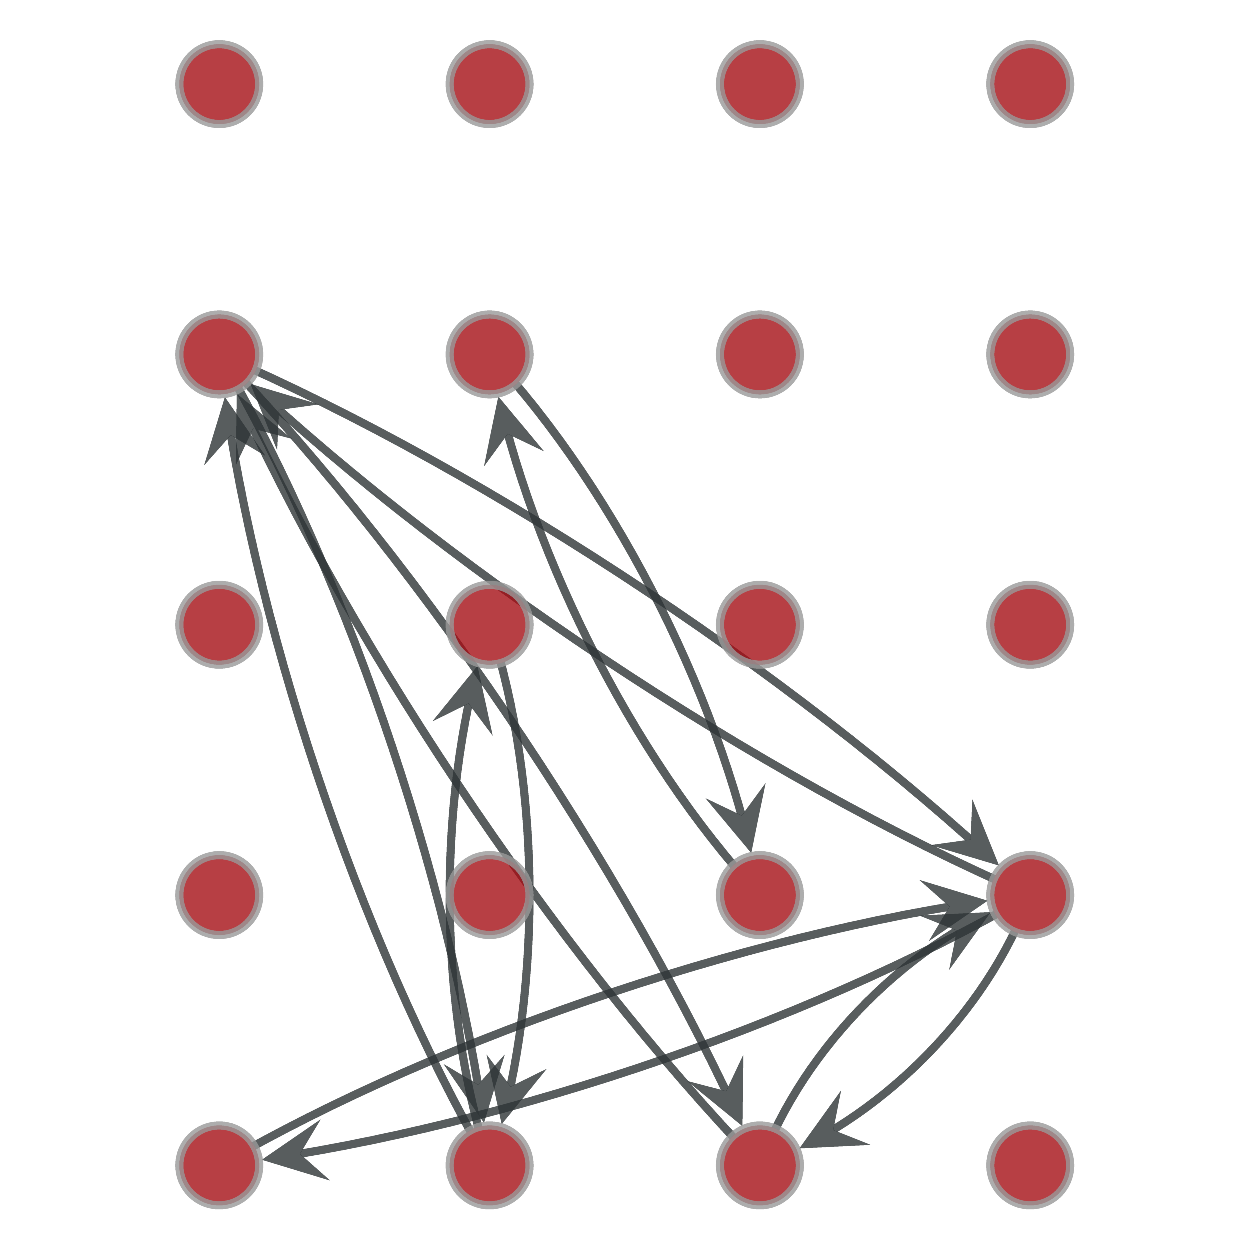
\includegraphics[height=4cm]{\MyPath/fig/1_firsthalf_.pdf}
		\caption{{\textbf{user 1}: 1\textsuperscript{st} half of the \mbox{observation period}}}
		\label{fig:evidence11}
	\end{subfigure}%
	\begin{subfigure}[]{0.495\textwidth}
		\centering
		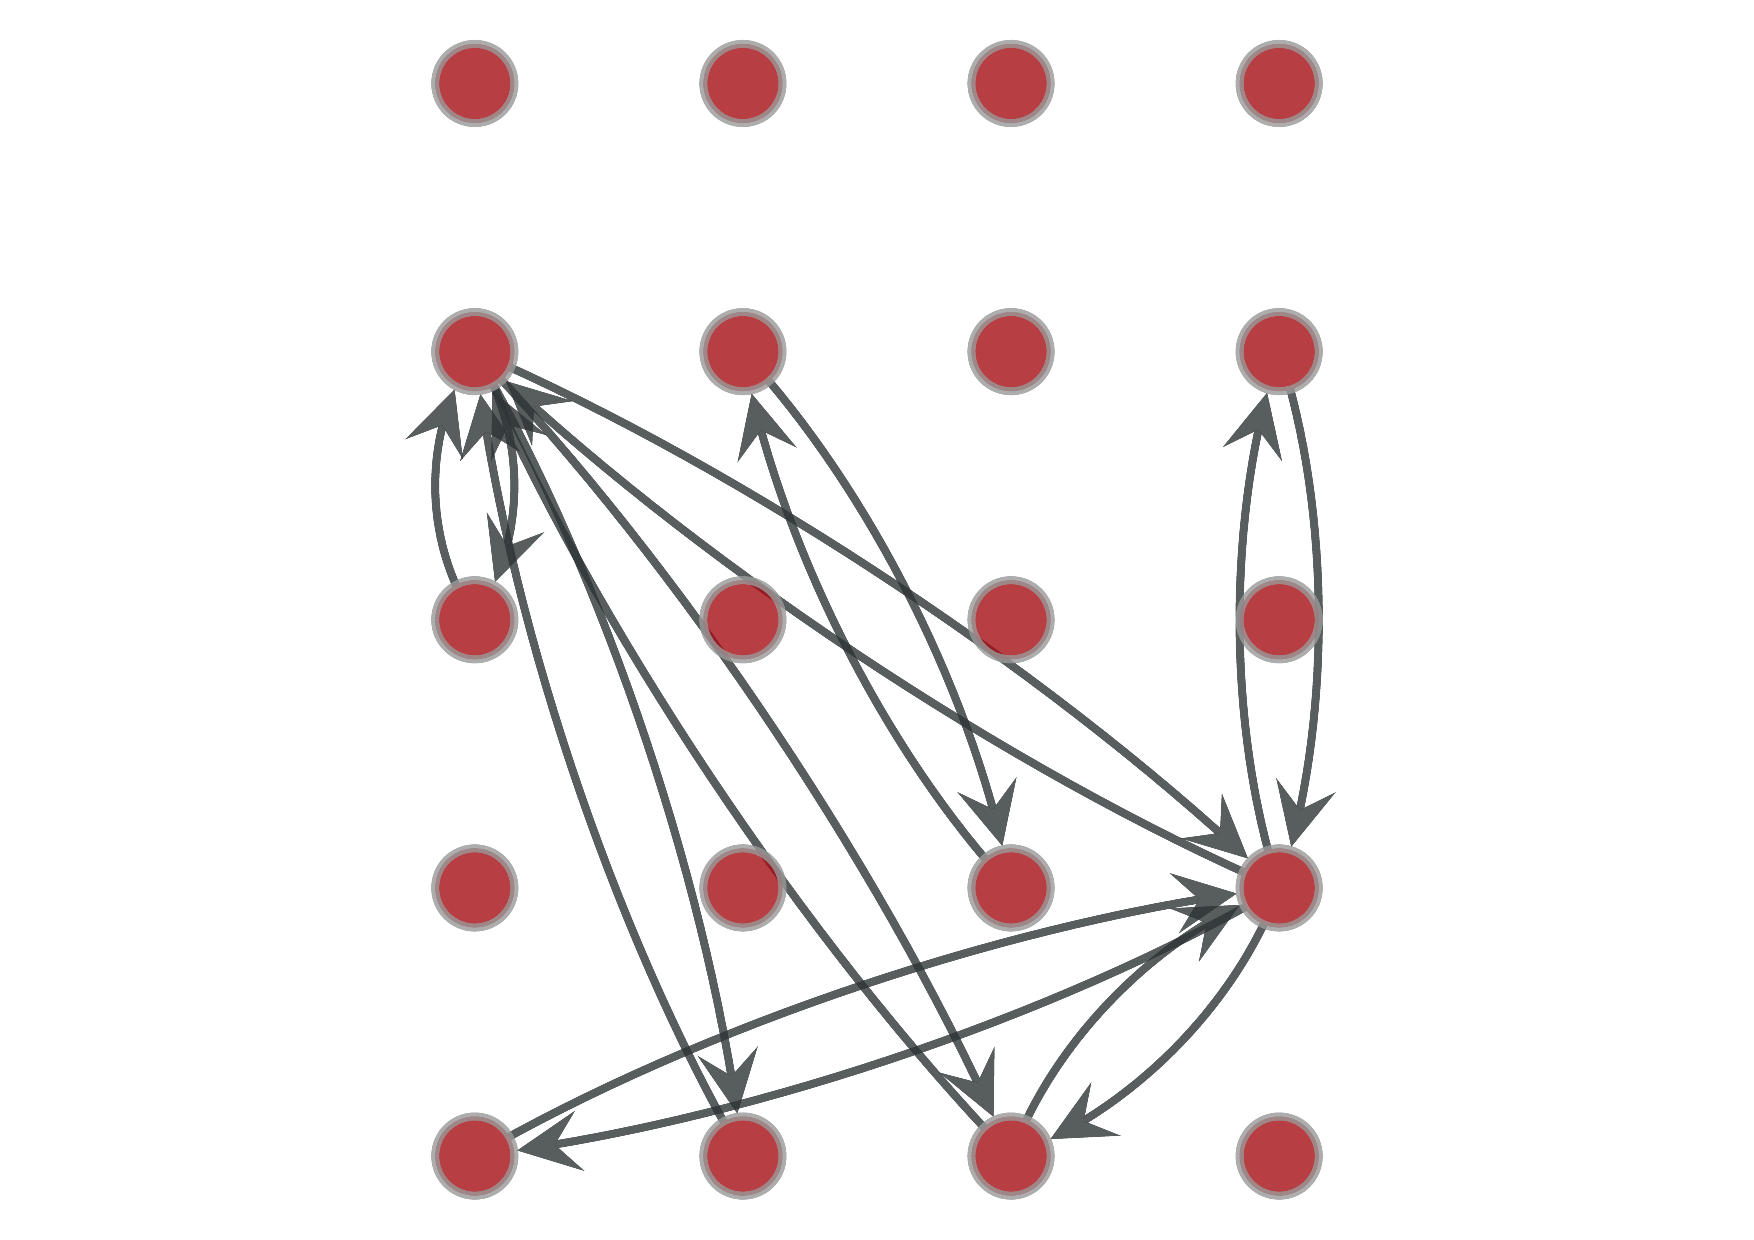
\includegraphics[height=4cm]{\MyPath/fig/1_secondhalf_.pdf}
		\caption{{\textbf{user 1}: 2\textsuperscript{nd} half of the \mbox{observation period}}}
		\label{fig:evidence12}
	\end{subfigure}%
	\\
	\begin{subfigure}[]{0.495\textwidth}
		\centering
		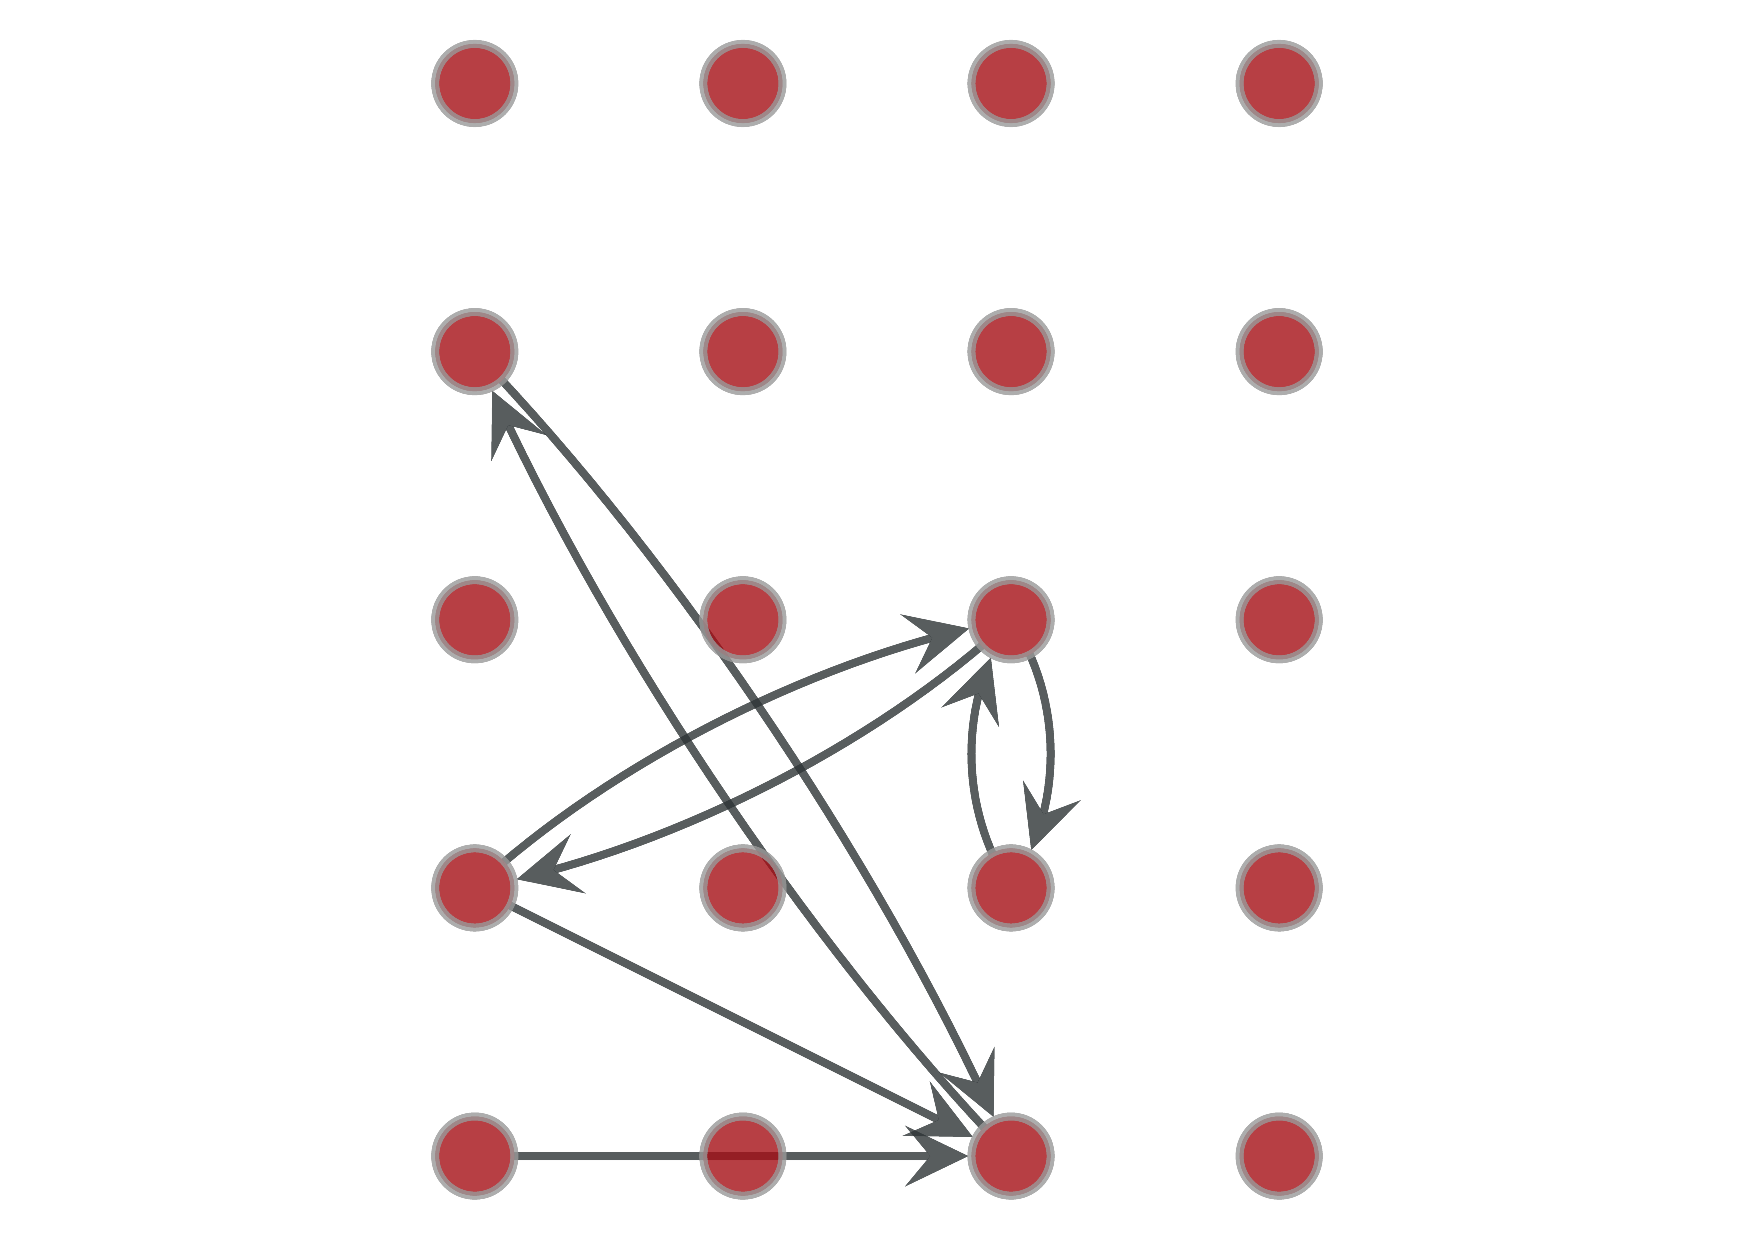
\includegraphics[height=4cm]{\MyPath/fig/2_firsthalf_.pdf}
		\caption{{\textbf{user 2}: 1\textsuperscript{st} half of the \mbox{observation period}}}
		\label{fig:evidence21}
	\end{subfigure}
	\begin{subfigure}[]{0.495\textwidth}
		\centering
		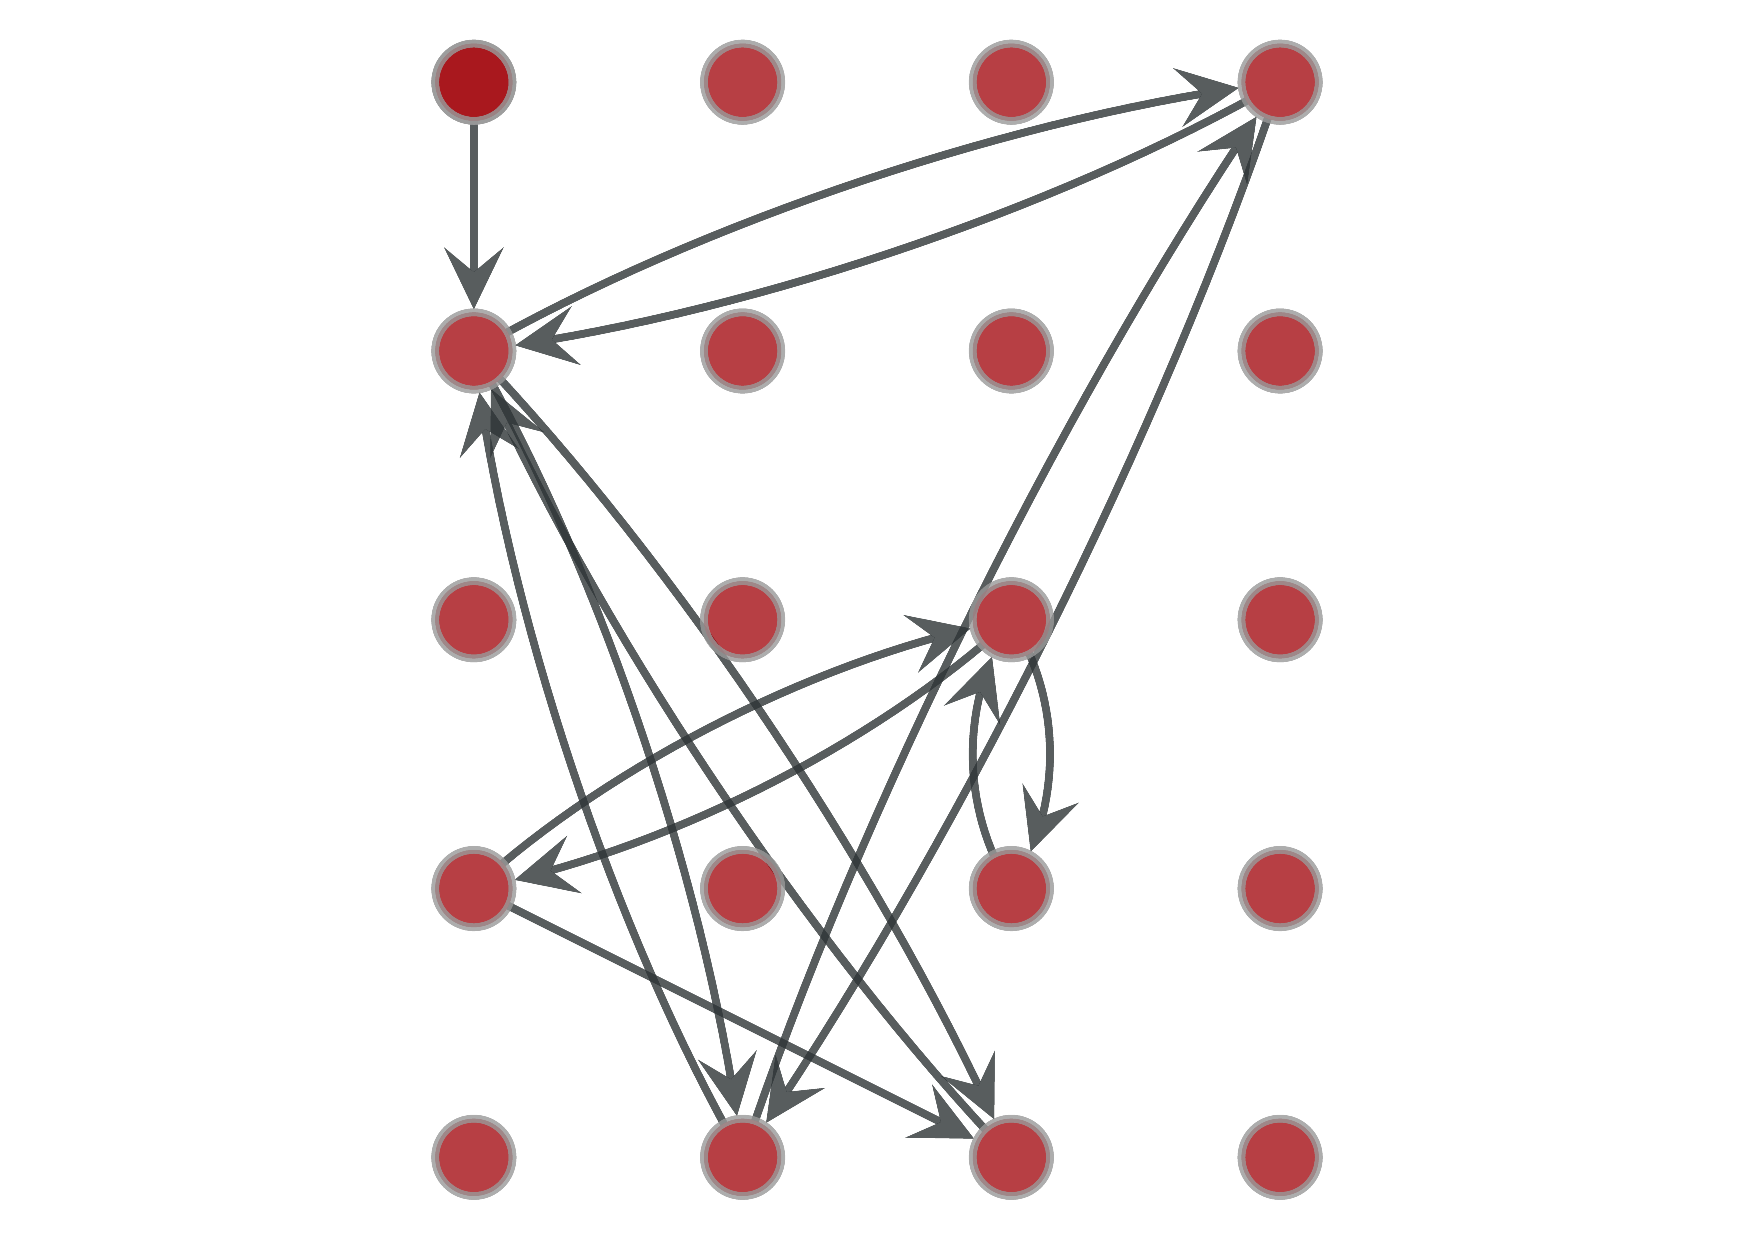
\includegraphics[height=4cm]{\MyPath/fig/2_secondhalf_.pdf}
		\caption{{\textbf{user 2}: 2\textsuperscript{nd} half of the \mbox{observation period}}}
		\label{fig:evidence22}
	\end{subfigure}
	\caption{{Top$-20$ networks for two random users from the Device Analyzer dataset.
  Depicted edges correspond to the $10\%$ most frequent transitions in the respective observation window.
  The networks show a high degree of similarity between the mobility profiles of the same user over the two observation periods.
  Moreover, the presence of single directed edges in the profile of \textbf{user 2} forms a discriminative pattern that allows us to distinguish \textbf{user\;2} from \textbf{user 1}.}}
	\label{fig:evidence}
\end{figure}
%\textcolor{red}{add a plot over a temporal graph of an individual justifying this hypothesis}


The basic premise of our deanonymization approach can be postulated as follows:

%\begin{tcolorbox}
\emph{
	The mobility of a person across different time periods is stochastic, but largely recurrent and stationary, and its expression at the level of the individual mobility network is discriminative enough to reduce a person's privacy within a population.}
%\end{tcolorbox}

For example, the daily commute to work corresponds to a relatively stable sequence of cell towers.
This can be expressed in the mobility network of the user as a persistent subgraph and forms a characteristic behavioural pattern that can be exploited for deanonymization of mobility traces.
Empirical evidence for our hypothesis is shown in~\cref{fig:evidence}.
For ease of presentation, in the figure, nodes between the disparate observation periods of the users can be cross-referenced. We assume that cross-referencing is not possible in our attack scenario, as locations are independently pseudonymized.

\subsubsection{Threat model \label{sec:threat-model}}

We assume that an adversary has access to a \emph{set of mobility networks} $ G \in \mcG_{\text{training}} $ \emph{with disclosed identities (or labels)} $l_{G} \in \mcL$
and a \emph{set of mobility networks} $ G' \in \mcG_{\text{test}} $ \emph{with undisclosed identities}
$ l_{G'} \in \mcL$.%

{Generally we can think of $ l_{G'} \in \mcJ \supset \mcL$ and assign some fixed probability mass to the labels $ l_{G'} \in \mcJ \setminus \mcL$.
However, here we make the \emph{closed world assumption} that the training and test networks come from the same population.
We make this assumption for two reasons: first, it is a common assumption in works on deanonymization and, second, we cannot directly update our beliefs on $ l_{G'} \in \mcJ \setminus \mcL$ by observing samples from $ \mcL$. }

We define a normalised similarity metric among the networks $ K: \mcG_{\text{training}} \times \mcG_{\text{test}} \rightarrow \mcR^+ $.
We hypothesize that a training and test mobility network belonging to the same person have common or similar connectivity patterns, thus a high degree of similarity.

The intention of an adversary is to deanonymize a given test network $ G' \in \mcG_{\text{test}} $, by appropriately defining a vector of probabilities over the possible identities in $ \mcL$.

An \textbf{uninformed adversary} has \emph{no information} about the networks of the population and, in the absence of any other side knowledge, the prior belief of the adversary about the identity of $ G' $ is a uniform distribution over all possible identities:
\[
	P\left(l_{G'}= l_{G_i}\right) = 1/|\mcL|, \mbox{ for every }  G_i \in \mcG_{\text{training}}.
\]

An \textbf{informed adversary} has \emph{access to the population of training networks} and can compute the pairwise similarities of $ G' $ with each $ G_{i} \in \mathcal{G}_{\text{training}} $ using a kernel function $K$. Hence the adversary can update her belief for the possible identities in $ \mathcal{L} $ according to the values of $K$.
Therefore, when the adversary attempts to deanonymize identities in the data, she assigns probabilities that follow a \emph{non-decreasing function} {of the computed pairwise similarity} of each label.
Denoting this function by $f$, we can write the updated adversarial probability estimate for each identity as follows:
\[
	P_K\left(l_{G'} =l_{G_i}| \mcG_{\text{training}}\right) =  \frac{f\left(K(G_i, G')\right)}{\displaystyle \sum_{j\in \mcL}  f\left(K(G_j, G')\right)},   \mbox{ for every }  G_i \in \mcG_{\text{training}}.
	\label{eq:adversarial_rule}
\]




\subsubsection{Privacy loss}

In the case of the uninformed adversary, the true label for any user is expected to have rank $ |\mcL|/2$. Under this policy, the amount of privacy for each user is proportional to the size of the population.

In the case of the informed adversary, knowledge of $ \mcG_\text{training} $ and the use of $ K $ will induce some non-negative \emph{privacy loss} which will result in the expected rank of user to be smaller than $ |\mcL|/2$. The privacy loss can be quantified as follows:
\[
	PL\left(G';\mcG_{\text{training}}, K\right) = \frac{P_K\left(l_{G'}= l_{G'_\text{true}}|\mcG_{\text{training}}\right)}{P\left(l_{G'}= l_{G'_\text{true}}\right)} -1
	\label{eq:privloss}
\]

A privacy loss equal to zero reflects no information gain compared to an uninformed adversary with no access to graphs with disclosed identities.

Let us assume that the users of our population generate distinct mobility networks.
As will be supported with empirical evidence in the next section, this is often the case in real-world \emph{cid} datasets of few thousand users even for small networks sizes (e.g. for top$-20$ networks in our dataset).
Under the above premise, the maximal privacy loss occurs when the presented test network is an identical copy of a training network of the same user which exists in the data of the adversary, \ie\ $ G' \in \mcG_\text{training}$.
This corresponds to a user deterministically repeating her mobility patterns over the observation period recorded in the test network.
In such a scenario, we could think that isomorphism tests are the most natural way to compute similarity; however, isomorphism tests will be useless in real-world scenarios, since the stochastic nature and noise inherent in the mobility networks of a user would make them non-isomorphic.
Maximal privacy loss reflects the discriminative ability of the kernel and cannot be exceeded in real-world datasets, where the test networks are expected to be noisy copies of the training networks existing in our system.
The step of comparing with the set of training networks adds computational complexity of $O(|\mcG_{\text{training}}|)$ to the similarity metric cost.

Moreover, our framework can naturally facilitate incorporating new data to our beliefs when multiple examples per individual exist in the training dataset.
For example, when multiple instances of mobility networks per user are available, we can use $k-$nearest neighbors techniques in the comparison of distances with the test graph.

\section{Data for analysis}

In this section we present an exploratory analysis of the dataset used in our experiments, highlighting statistical properties of the data and empirical results regarding the structural anonymity of the generated state connectivity networks.

\subsection{Data description}

We evaluate our methodology on the Device Analyzer dataset~\citep{Wagner2014}. Device Analyzer contains records of smartphone usage collected from over $ 30,000 $  study participants around the globe.
Collected data include information about system status and parameters, running background processes, cellular and wireless connectivity.
For privacy purposes, released \emph{cid} information is given a unique pseudonym separately for each user, and contains no geographic, or semantic, information concerning the location of users.
Thus we cannot determine geographic proximity between the nodes, and the location data of two users cannot be directly aligned.

For our experiments, we analysed \emph{cid} information collected from $1,500$ handsets with the largest number of recorded location datapoints in the dataset.
\cref{fig:num_of_days} shows the observation period for these handsets; note that the mean is greater than one year but there is lot of variance across the population.
We selected these $1,500$ handsets in order to examine the reidentifiability of devices with rich longitudinal mobility profiles.
This allowed us to study the various attributes of individual mobility affecting privacy in detail.
As mentioned in the previous section, the cost of computing the adversarial posterior probability for the deanonymization of a given unlabeled network scales linearly with the population size.

\begin{figure*}[!t]
	\centering
	\begin{subfigure}[!t]{0.47\textwidth}
		\centering		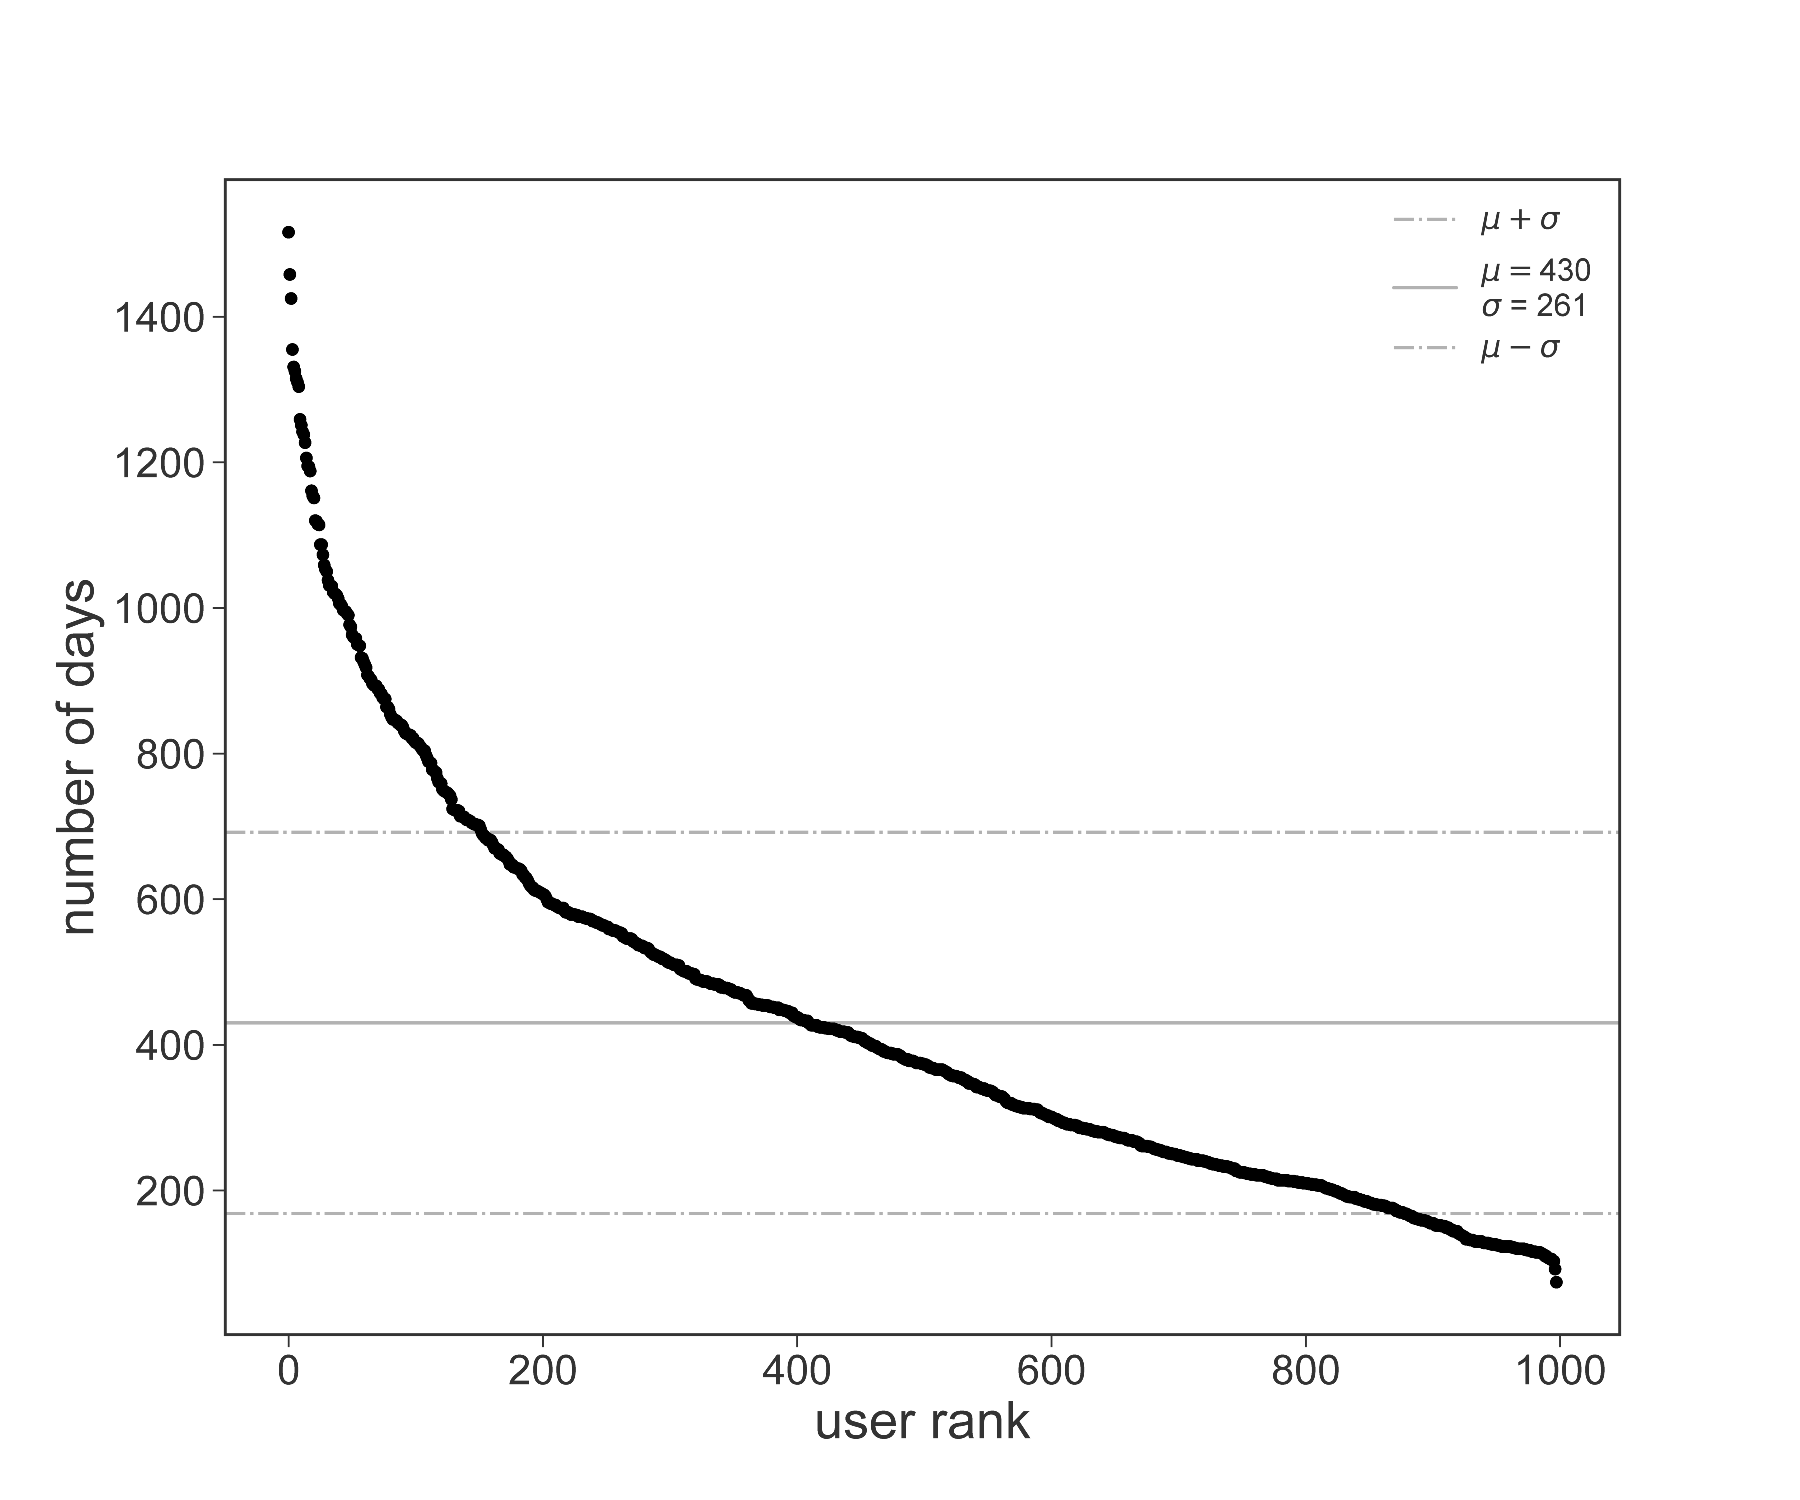
\includegraphics[width=0.9\textwidth]{\MyPath/fig/observation_window_.pdf}
		\caption{}
		\label{fig:num_of_days}
	\end{subfigure}%
	\begin{subfigure}[!t]{.47\textwidth}
		\centering
		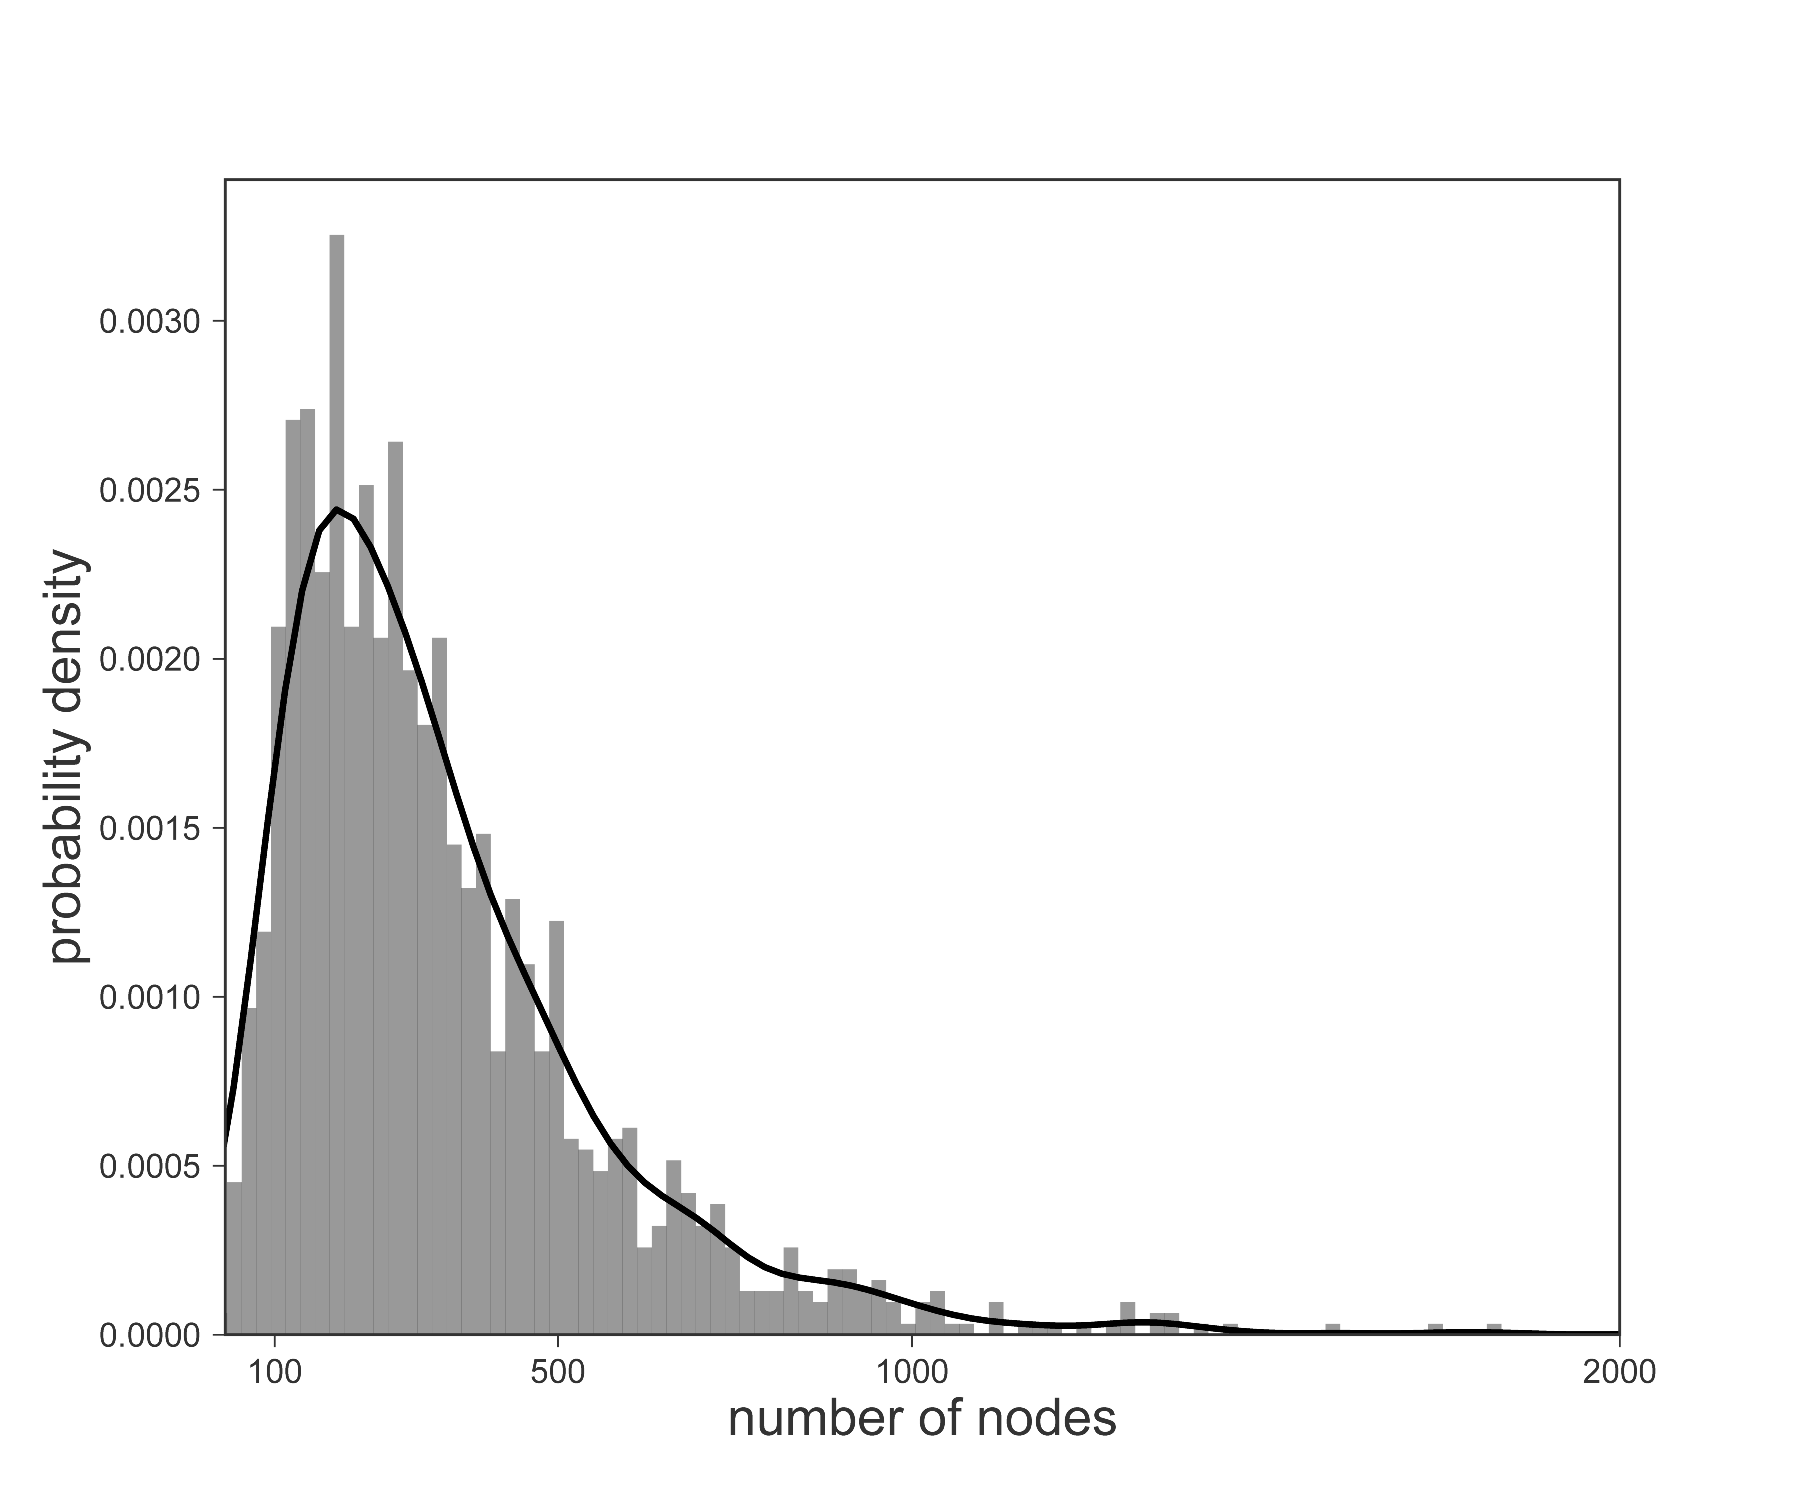
\includegraphics[width=0.9\textwidth]{\MyPath/fig/unnorm_full_graphspdf_netsize_.pdf}
		\caption{}
		\label{fig:sizes}
	\end{subfigure}%
	\\
	\begin{subfigure}[!t]{0.47\textwidth}
		\centering
		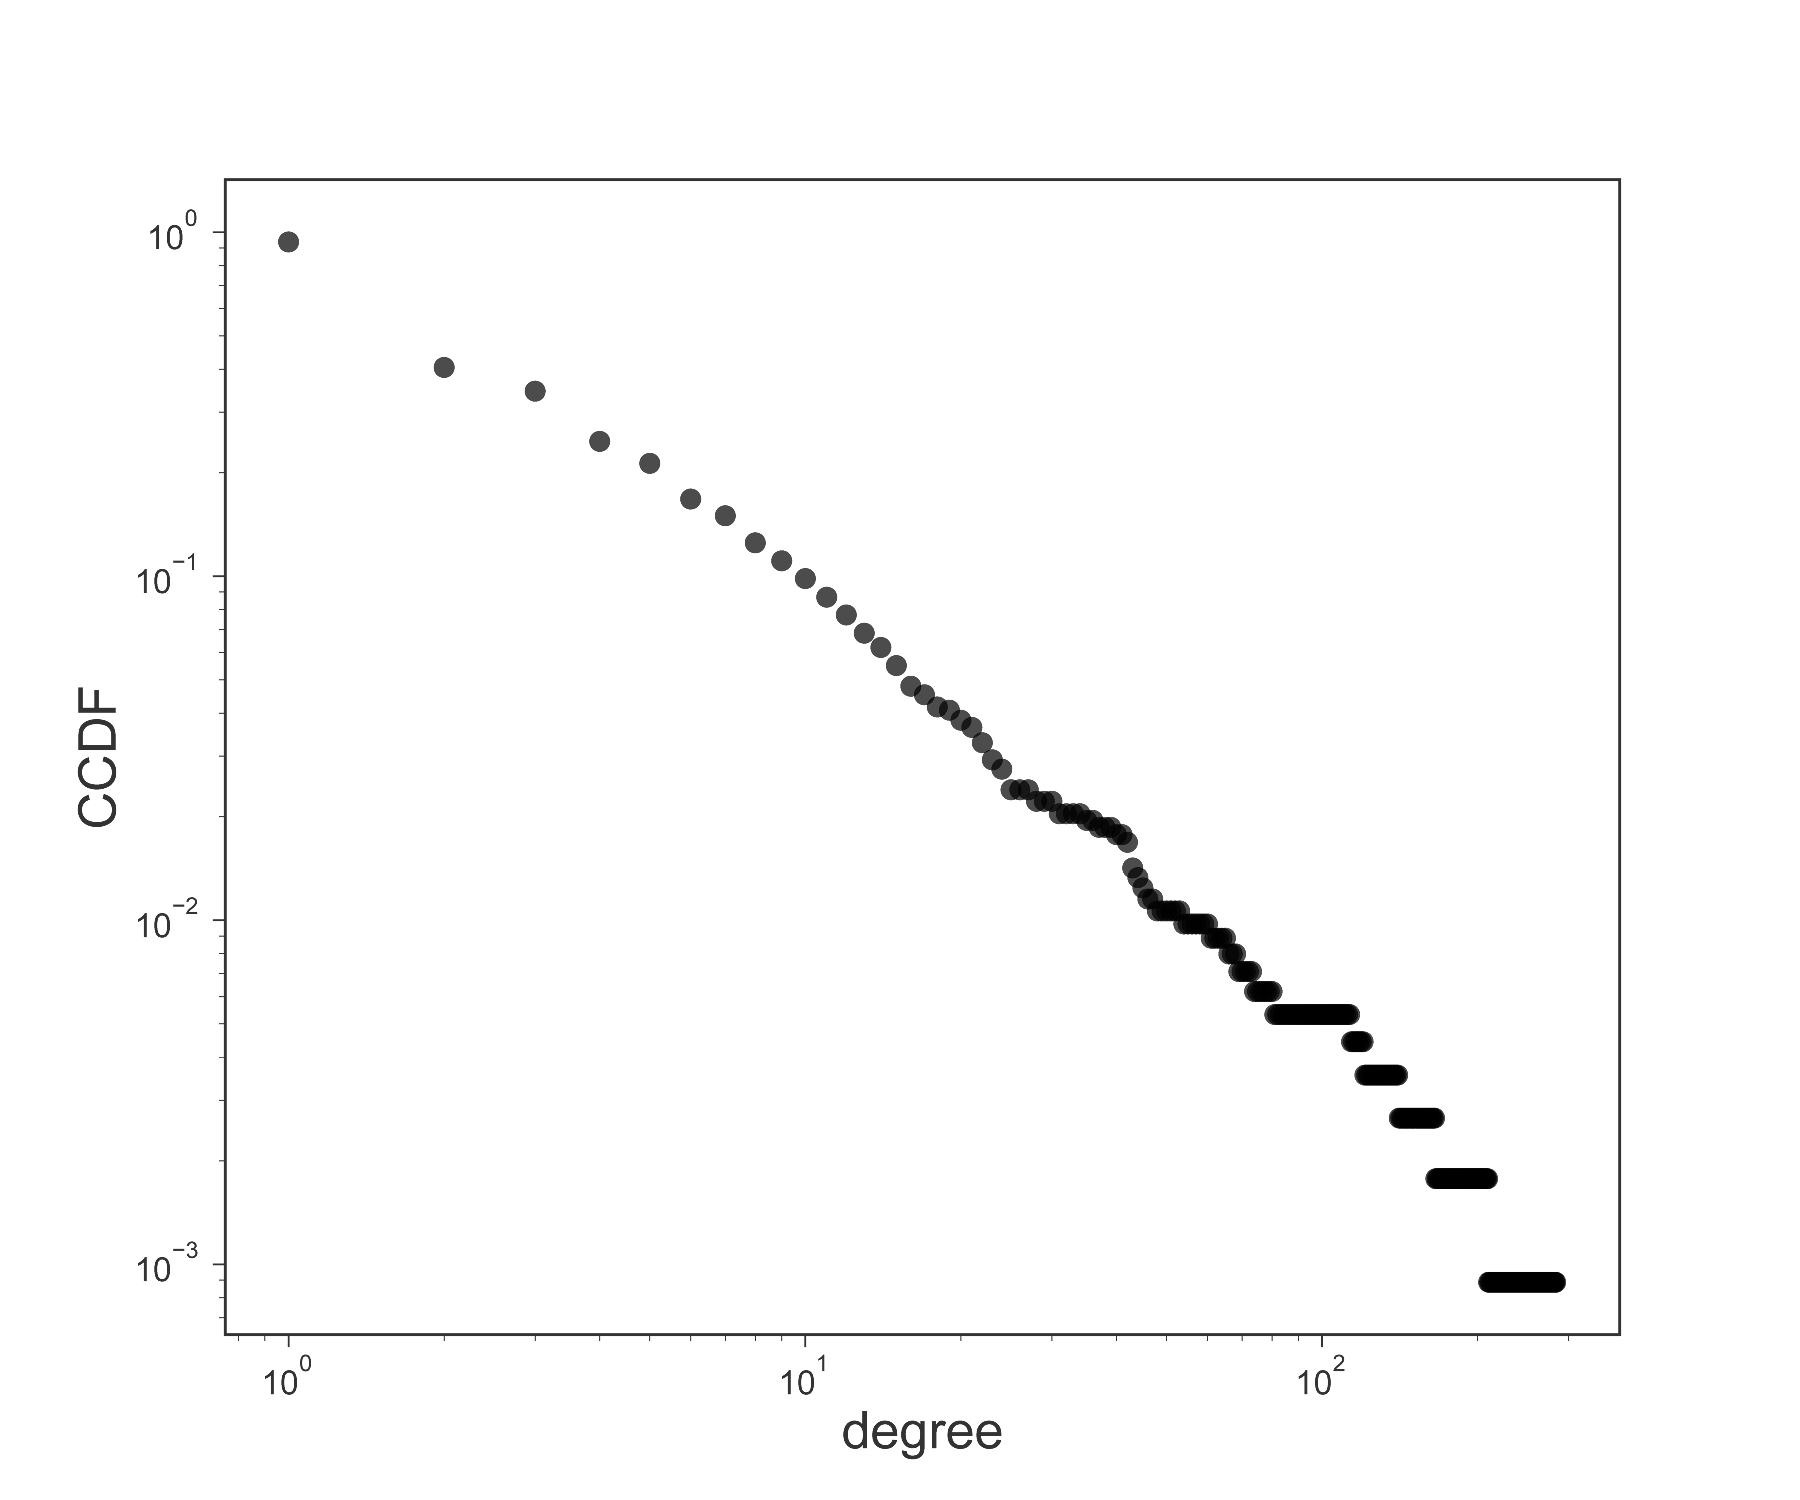
\includegraphics[width=0.9\textwidth]{\MyPath/fig/183_degree_ccdf_.pdf}
		\caption{}
		\label{fig:ccdf}
	\end{subfigure}
	\begin{subfigure}[!t]{0.47\textwidth}
		\centering
		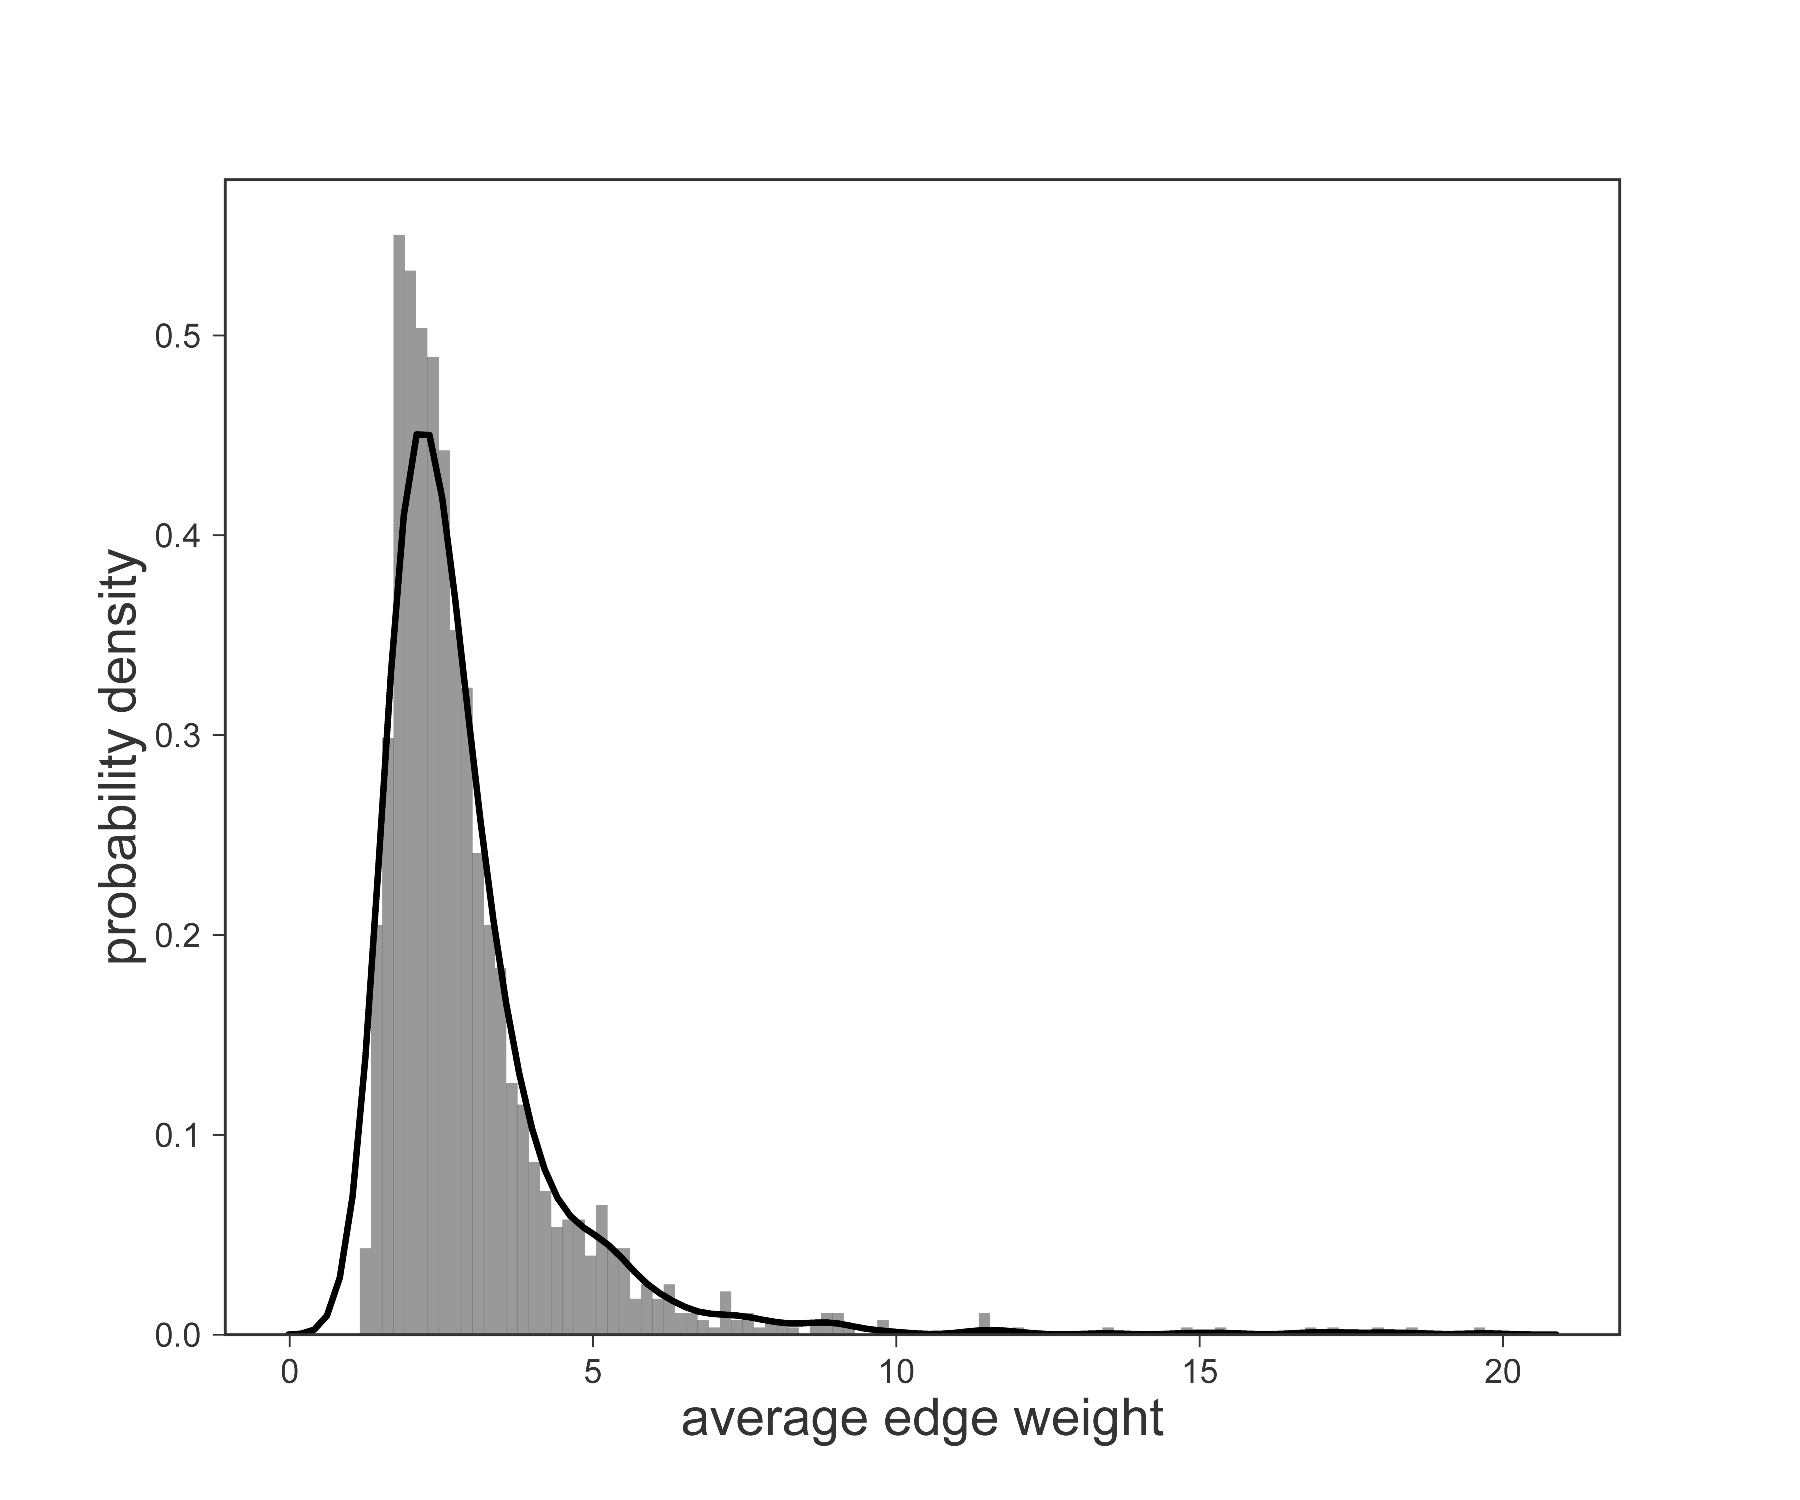
\includegraphics[width=0.9\textwidth]{\MyPath/fig/unnorm_full_graphspdf_avg_edge_weight_.pdf}
		\caption{}
		\label{fig:avg_edge_weight}
	\end{subfigure}
	\caption{Empirical statistical findings of the Device Analyzer dataset. (a)~Distribution of the observation period duration. (b)~Normalized histogram and probability density estimate of network size for the full mobility networks over the population. (c)~Complementary cumulative distribution function (\emph{CCDF}) for the node degree in the mobility network of a typical user from the population, displayed on log-log scale. (d)~Normalized histogram and probabilty density of average edge weight over the networks.}
	\label{fig:eda}
\end{figure*}

\subsection{Mobility networks construction\label{sec:mobility-net-construct}}

\begin{figure*}[t]
	\centering
	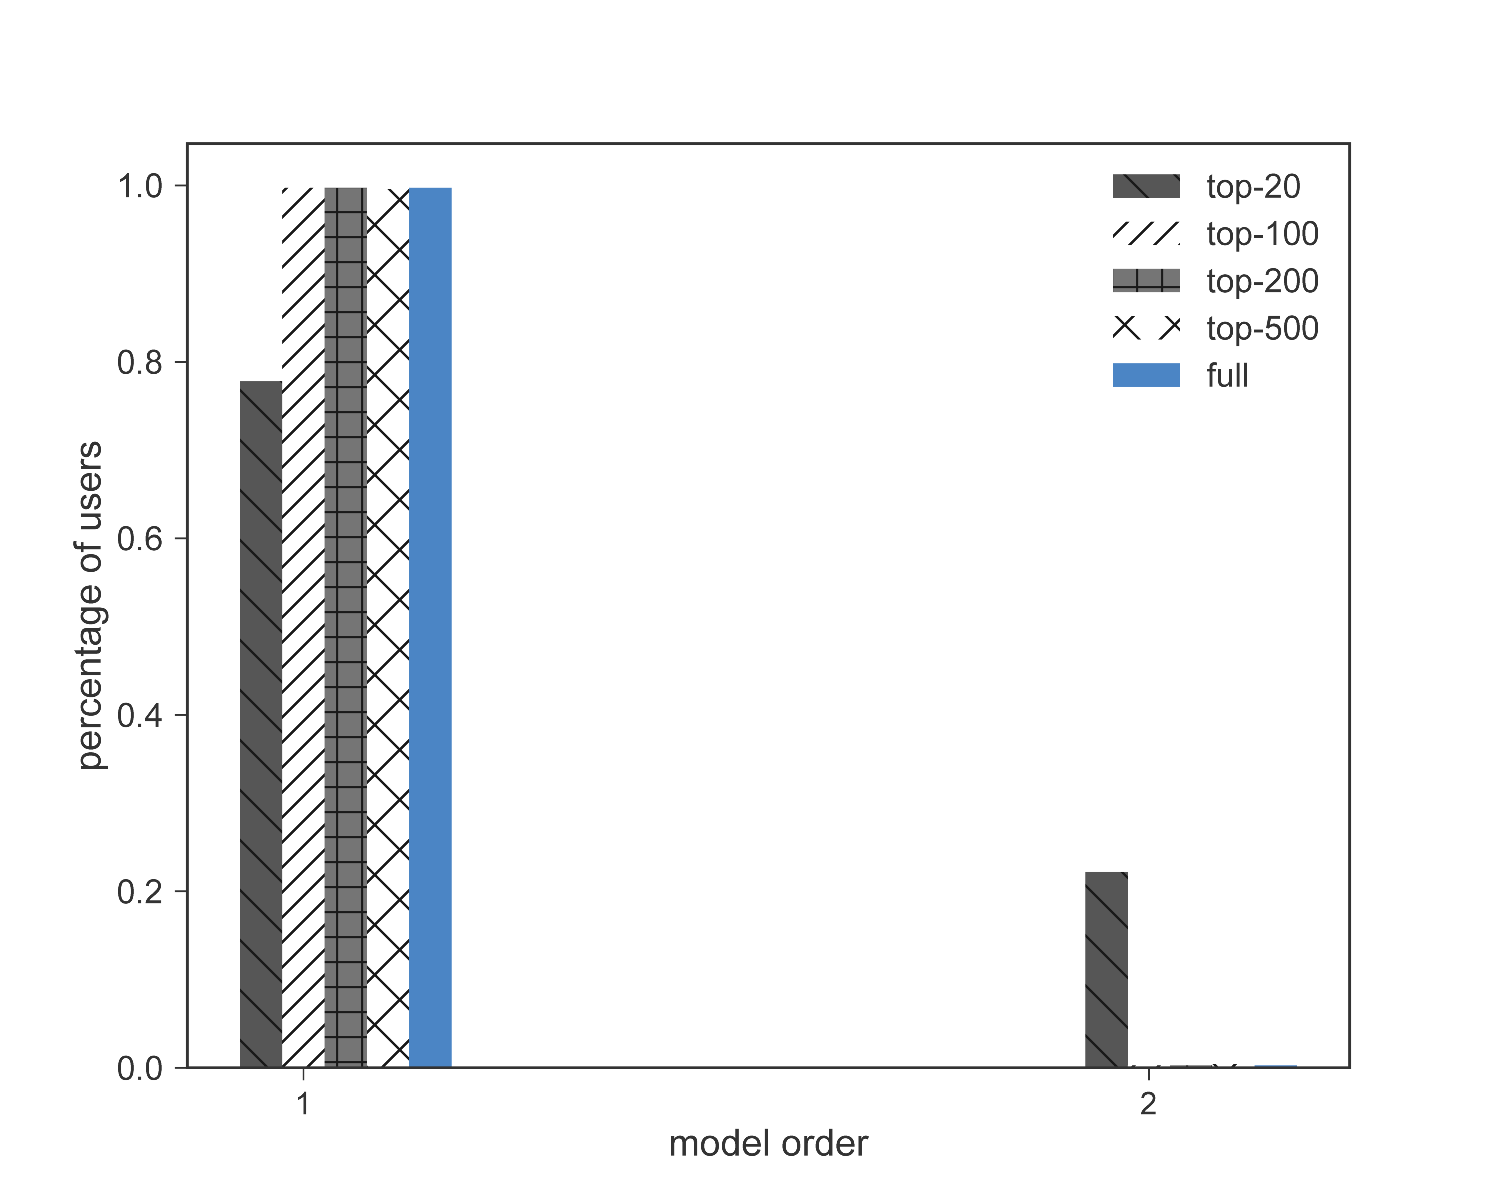
\includegraphics[totalheight=8cm]{\MyPath/fig/model_selection_.pdf}
	\caption{{Optimal order for increasing number of locations.}}
	\label{fig:model_selection}
\end{figure*}

We began by selecting the optimal order of the network representations derived from the mobility trajectories of the $1,500$ handsets selected from the Device Analyzer dataset.
We first parsed the \emph{cid} sequences from the mobility trajectories into mobility networks.
In order to remove \emph{cid}s associated with movement, we only defined nodes for \emph{cid}s which were visited by the handset for at least 15 minutes.
Movements from one \emph{cid} to another were then recorded as edges in the mobility network.

As outlined in~\cref{sec:graph-k-anonymity}, we analysed the pathways of the Device Analyzer dataset during the entire observation period, applying the model selection method of~\textcite{scholtes2017network}.\footnote{\url{https://github.com/IngoScholtes/pathpy}}
This method tests graphical models of varying orders and selects the optimal order by balancing the model complexity and the explanatory power of observations.

We tested higher-order models up to order three. In the case of top$-20$ mobility networks, we found routine patterns in the mobility trajectories were best explained with models of order two for more than 20$\%$ of the users. However, when considering top$-100$, top$-200$, top$-500$ and full mobility networks, we found that the optimal model for our dataset has order one for more than $ 99\% $ of the users; see~\cref{fig:model_selection}. In other words, when considering mobility trajectories which visit less frequent locations in the graph, the overall increase in likelihood of the data for higher-order models cannot compensate for the complexity penalty induced by the larger state space. Hence, while there might still be regions in the graph which are best represented by a higher-order model, the optimal order describing the entire graph is one. Therefore we use a model of order one in the rest of this chapter.

\subsection{Data properties and statistics} \label{sec:data-stats}

\begin{table*}[!t]
	\centering 
		\resizebox*{\textwidth}{!}{
			\begin{tabular}{| c | c | c | c | c | c | c | c | c |}
				\hline
				\textbf{Networks} & \vtop{\hbox{\strut \;\;\;\textbf{\# of}}\hbox{\strut \textbf{networks}}}  &  \vtop{\hbox{\strut \textbf{Num. of}}\hbox{\strut \textbf{nodes,~avg.}}}  &  \vtop{\hbox{\strut \textbf{Edges,}}\hbox{\strut \;\;\;\textbf{avg.}}} & \vtop{\hbox{\strut \textbf{Density,}}\hbox{\strut \;\;\;\textbf{avg.}}} & \vtop{\hbox{\strut \;\;\;\;\;\;\textbf{Avg.}}\hbox{\strut \textbf{clust. coef.}}} & \vtop{\hbox{\strut \textbf{Diameter,}}\hbox{\strut \;\;\;\;\;\;\textbf{avg.}}}  & \vtop{\hbox{\strut \;\;\;\;\;\textbf{Avg.}}\hbox{\strut \textbf{short.~path}}} & \vtop{\hbox{\strut \textbf{Recurrence}}\hbox{\strut \;\;\;\;\;\textbf{rate~($\%$)}}}   \\
				\hline
				\text{top$-50$ locations}& $1,500$ & $49.9\pm1.3$  & $236.6\pm78.1$ & $0.19\pm0.06$ & $0.70\pm0.07$ & $3.42\pm0.86$  & $1.93\pm0.20$ & $84.7\pm5.6$\\
				\hline
				\text{top$-100$ locations}& $1,500$ & $98.3\pm7.9$   & $387.1\pm144.7$ & $0.08\pm0.03$ & $0.60\pm0.10$ & $4.67\pm1.48$  & $2.33\pm0.40$& $78.3\pm7.8$\\
				\hline
				\text{top$-200$ locations}& $1,500$ & $179.2\pm37.8$ & $548.2\pm246.1$ & $0.04\pm0.02$ & $0.47\pm0.12$ & $7.52\pm4.21$  & $3.07\pm1.18$ &$73.0\pm9.9$\\
				\hline
				\text{full } & $1,500$ & $334.6\pm235.8$  & $741.6\pm527.3$ & $0.02\pm0.02$ & $0.33\pm0.09$ & $15.98\pm10.18$  & $4.84\pm2.93$ & $68.8\pm12.3$\\
				\hline
			\end{tabular}	
		}\caption{Summary statistics of mobility networks in the Device Analyzer dataset.}
		\label{tab:summary-statistics}
\end{table*}	



In~\cref{tab:summary-statistics} we provide a statistical summary of the original and the pruned versions of the mobility networks. We observe that allowing more locations in the network implies an increase in the variance of their statistics, and leads to smaller density, larger diameter and larger average shortest-path values.

A \emph{recurrent edge traversal} in a mobility network occurs when a previously traversed edge is traversed for a second or subsequent time.
We then define \emph{recurrence rate} as the percentage of edge traversals which are recurrent.
We find that mobility networks display a high recurrence rate, varying from  $68.8\%$ on average for full networks to $84.7\% $ for the top$-50$ networks, indicating that the mobility of the users is mostly comprised of repetitive transitions between a small set of nodes in a mobility network.

\cref{fig:sizes} displays the normalized histogram and probability density estimate of network size for full mobility networks.
We observe that sizes of few hundred nodes are most likely in our dataset, however mobility networks of more than $1,000$ nodes also exist.
Reducing the variance in network size will be proved helpful in cross-network similarity metrics, hence we also consider truncated versions of the networks.

As shown in~\cref{fig:ccdf}, the parsed mobility network of a typical user is characterized by a \emph{heavy-tailed degree distribution}. We observe that a small number of locations have high degree and correspond to dominant states for a person's mobility routine, while a large number of locations are only visited a few times throughout the entire observation period and have a small degree.

 \cref{fig:avg_edge_weight} shows that the estimated probability distribution of average edge weight.
 This peaks in the range from two to four, indicating that many transitions captured in the full mobility network are rarely repeated. However, most of the total weight of the network is attributed to the tail of this distribution, which corresponds to the edges that the user frequently repeats.

\subsection{Anonymity clusters on top$-N$  networks}\label{sec:anonymity-clusters}


We examine to what extent the heterogeneity of users mobility behaviour can be expressed in the topology of the state connectivity networks.
For this purpose, we generate the isomorphism classes of the top$-N$ networks of our dataset for increasing network size $ N $.
We then compute the graph $k-$anonymity of the population and the corresponding identifiability set.
This analysis demonstrates empirically the privacy implications of releasing anonymized users pathway information at increasing levels of granularity.

Before presenting our findings on the Device Analyzer dataset, we will perform a theoretical upper bound analysis on the identifiability of a population, by finding the maximum number of people that can be distinguished by networks of size $ N $.
This corresponds to the number of non-isomorphic graphs with $ N $ nodes.

\begin{table*}[!t]
	\centering
	\resizebox*{0.7\textwidth}{!}{
		\begin{tabular}{|c|c|c|c|c|c|c|}
			\hline
			\textbf{N}             & 4    & 5           & 6           & 7            & 8             & 9         \\ \hline
			\textbf{\# undirected} & 11   & 34          & 156         & 1,044         & 12,346         & 274,668    \\ \hline
			\textbf{N}             & 4    & \multicolumn{2}{c|}{5}    & \multicolumn{2}{c|}{6}       & 7         \\ \hline
			\textbf{\# directed}   & 2,128 & \multicolumn{2}{c|}{9,608} & \multicolumn{2}{c|}{1,540,944} & 882,033,440 \\ \hline
		\end{tabular}
	}\caption{Sequences of non-isomorphic graphs for undirected and directed graphs of increasing size.}
	\label{tab:graphsenumeration}
\end{table*}

Currently the most efficient way of enumerating  non-isomorphic graphs is by using the algorithm of~\textcite{McKay}, implemented in the package~\texttt{nauty}.\footnote{\url{http://pallini.di.uniroma1.it/}}~\cref{tab:graphsenumeration} presents the enumeration for undirected and directed non-isomorphic graphs of increasing size. We observe that there exist $12,346$ undirected graphs with $8$ nodes and $9,608$ directed graphs with $5$ nodes. In other words, finding the top$-8$ places for each person is the smallest number which could produce unique graphs for each person in our sample of $1,500$ individuals; this reduces to $5$ when directionality is taken into account. Moreover, we find that top$-12$ undirected and top$-8$ directed networks are sufficient to enable each human on the planet to be represented by a different graph, assuming world population of $7.6$B.

Next we present the results of our analysis on the Device Analyzer data.
As observed in~\cref{fig:k_an}, \emph{sparsity arises in a mobility network even for very small $ N $}.
In particular, in the space of undirected \emph{top$-4$} location networks, there is already a cluster with only $ 3 $ members, while for all $ N > 4 $ there always exist isolated isomorphic clusters.
\emph{$ k-$anonymity} decreases to $ 1 $ even for $ N=3 $ when considering directionality.
Moreover, the \emph{identifiability set} dramatically increases with the size of network: approximately $ 60\% $ of the users are uniquely identifiable from their top$-10$ location network.
This percentage increases to $93\%$ in directed networks.
For the entire population of the $ 1,500 $ users, we find that 15 and 19 locations suffice to form uniquely identifiable directed and undirected networks respectively.

The difference between our empirical findings and our theoretical analysis suggests that large parts of the top$-N$ networks are common to many people.
This can be attributed to patterns that are widely shared (e.g.\ the trip from work to home, and from home to work).

\begin{figure*}[!t]
	\begin{subfigure}[t]{0.49\textwidth}
		\centering
		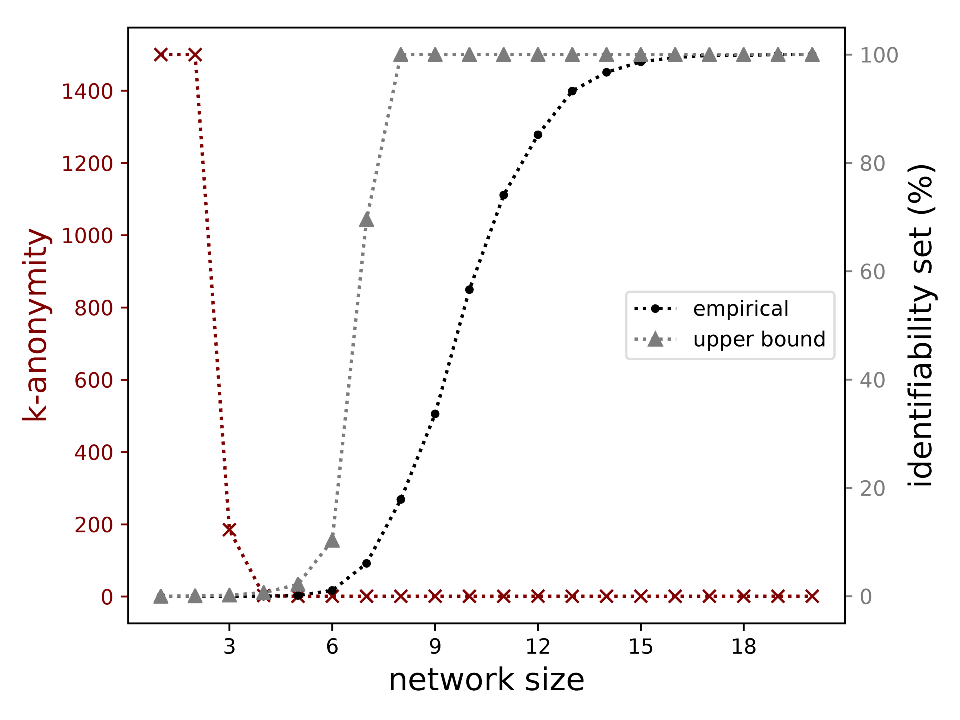
\includegraphics[height=5.5cm]{\MyPath/fig/k_anonymity_undirected_.pdf}
		\caption{\centering {Undirected top$-N$ networks.}}
		\label{fig:k_an_un}
	\end{subfigure}%
	\begin{subfigure}[t]{0.49\textwidth}
		\centering
		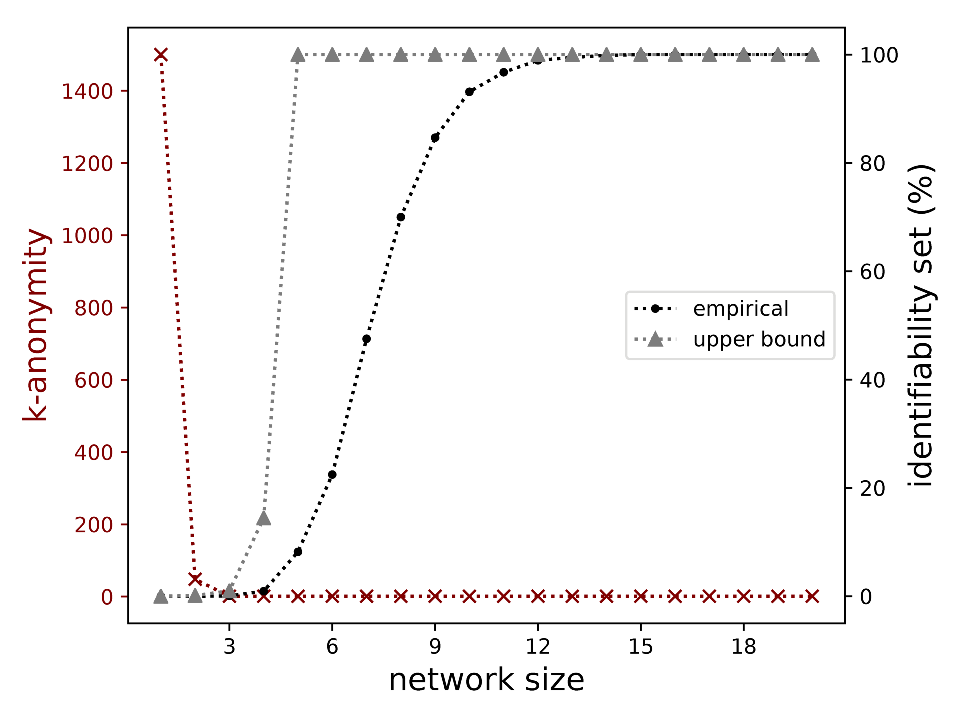
\includegraphics[height=5.5cm]{\MyPath/fig/k_anonymity_dir_.pdf}
		\caption{\centering {Directed top$-N$ networks.}}
		\label{fig:k_an_dir}
	\end{subfigure}%
	\caption{{Identifiability set and $k-$anonymity for undirected and directed top$-N$ mobility networks for increasing number of nodes. Displayed is also the theoretical upper bound of identifiability for networks with $ N $ nodes.}
	}
	\label{fig:k_an}
\end{figure*}

\begin{figure*}[!t]
	\begin{subfigure}[t]{0.49\textwidth}
		\centering
		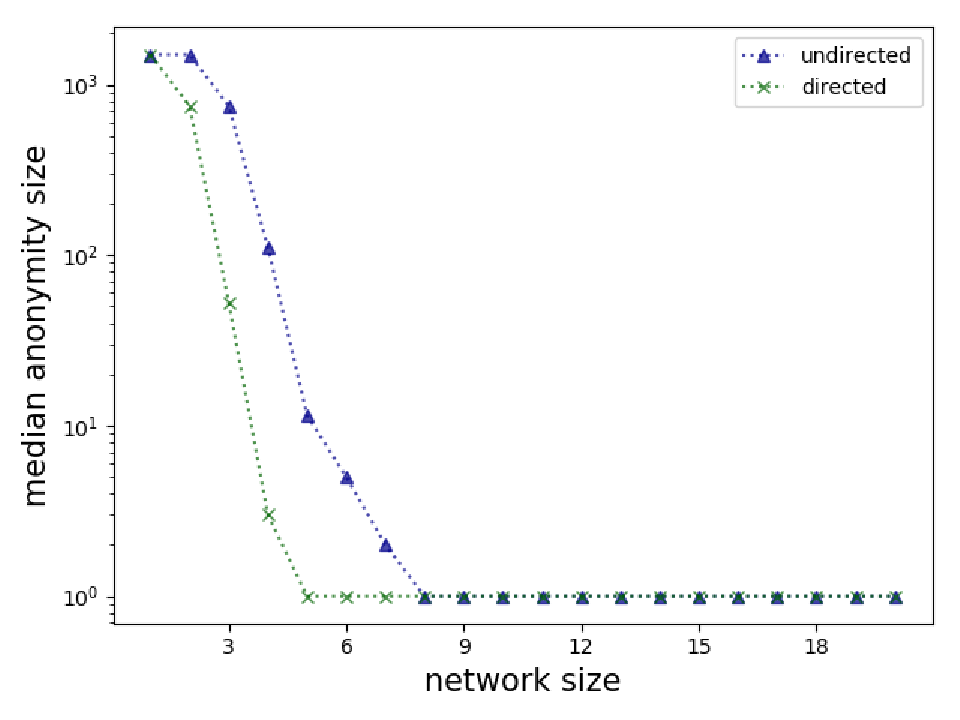
\includegraphics[height=5cm]{\MyPath/fig/median_k_anonymity_.pdf}
		\caption{\centering {Median anonymity size.}}
		\label{fig:k_an_med}
	\end{subfigure}
	\begin{subfigure}[t]{0.49\textwidth}
		\centering
		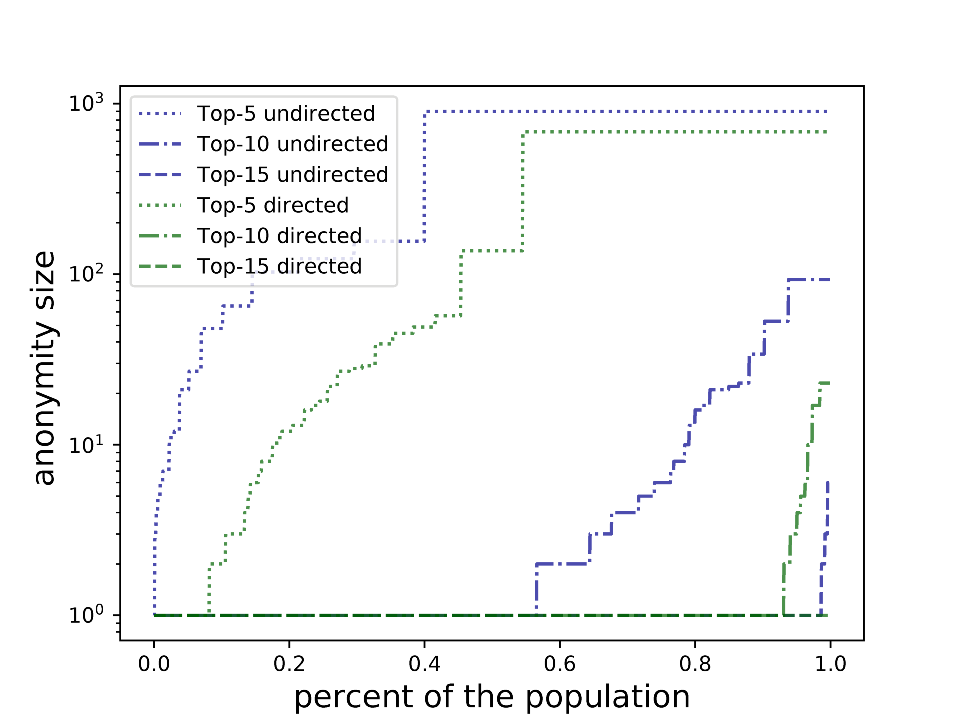
\includegraphics[height=5.5cm]{\MyPath/fig/anonymity_distribution_.pdf}
		\caption{\centering {Cumulative distribution of the anonymity size.}}
		\label{fig:anon_distribution}
	\end{subfigure}
	\caption{{Anonymity size statistics over the population of top$-N$ mobility networks for increasing network size.}}
	\label{fig:k_an_stats}
\end{figure*}

 \cref{fig:k_an_stats} shows some additional statistics of the anonymous isomorphic clusters formed for varying network sizes.
 Median anonymity becomes one for network sizes of five and eight in directed and undirected networks respectively; see~\cref{fig:k_an_med}.
 In~\cref{fig:anon_distribution} we observe that the population arranges into clusters with small anonymity even for very small network sizes: around $5\%$  of the users have at most $10$-anonymity when considering only five locations in their network, while this percentage increases to $80\%$ and $100\% $ for networks with $10$ and $15$ locations.
 This result confirms that anonymity is even harder when the directionality of edges are provided, since the space of directed networks is much larger than the space of the undirected networks with the same number of nodes.

 The above empirical results indicate that the diversity of individuals mobility is reflected in the network representations we use, thus we can meaningfully proceed to discriminative tasks on the population of mobility networks.
\section{Evaluation of privacy loss in longitudinal mobility traces}\label{sec:pl-evaluation}

In this section we empirically quantify the privacy leakage implied by the information of longitudinal mobility networks for the population of users in the Device Analyzer dataset.
For this purpose we undertake experiments in graph set matching using different kernel functions, and assume an adversary has access to a variety of mobility network information.

\subsection{Experimental setup}

For our experiments we split the \emph{cid} sequences of each user into two sets: the \emph{training} sequences where users' identities are disclosed to the adversary, and the \emph{test} sequences where user identities are undisclosed to the adversary, and are used to quantify the success of the adversarial attack.
Therefore each user has two mobility networks: one derived from the training sequences, and one derived from the test sequences.
The objective of the adversary is to successfully match every test mobility network with the training mobility network representing the same underlying user.
To do so, the adversary computes the pairwise distances between training mobility networks and test mobility networks.
We partitioned \emph{cid} sequences of each user by time, placing all \emph{cid}s before the partition point in the training set, and all subsequent \emph{cid}s into the test set.
We choose the partition point separately for each user as a random number from the uniform distribution with range $ 0.3 $ to $ 0.7 $.

\subsection{Mobility networks \& kernels}

We computed the pairwise distances between training and test mobility networks using kernels from the categories described in~\cref{sec:methodology}.
Node attributes are supported in the computation of Weisfeiler-Lehman and Shortest-Path kernel.
Thus, in this part of the study, we augmented the individual mobility networks with categorical features, to add some information about the different roles of nodes in users' mobility routine.
Such attributes are computed independently for each user on the basis of the topological information of each network.
After experimenting with several schemes, we obtained the best performance on the kernels when dividing locations into three categories with respect to the frequency in which each node is visited by the user.
Concretely, we computed the distribution of users' visits to locations and added the following values to the nodes:

\begin{equation*}
	a_{c=3}\left(v_i^u\right):=
	\begin{cases}
		 3, &  \mbox{if } v_i^u \in \mbox{top$-20\%$ locations of } u  \\
		 2, &  \mbox{if } v_i^u  \notin \mbox{top$-20\%$ locations of }  u   \mbox{ and }  v_i^u \in \mbox{top$-80\%$ locations}\\
		 1, &  \mbox{otherwise}.
	\end{cases}
\end{equation*}

This scheme allowed a coarse, yet informative, characterisation of locations in users' networks, which was robust to the variance in the frequency of visits between the two observation periods. In addition, we removed $40\%$ of edges with the smallest edge weights and retained only the largest connected component for each user.


Due to its linear complexity, the computation of the Weisfeiler-Lehman kernel could scale over entire mobility networks.
However, we had to reduce the network size in order to apply the Shortest-Path kernel.
This was done using top$-N$ networks for varying size $N$.



\subsection{Evaluation}

We evaluated graph kernels functions from the following categories:
\begin{itemize}
	\item \emph{DSP}$_{N}$: Deep Shortest-Path kernel on top$-N$ network
	\item \emph{DWL}$_{N}$: Deep Weisfeiler-Lehman kernel on top$-N$ network
	\item \emph{DD}: Degree Distribution kernel through Gaussian RBF
	\item \emph{WD}: Weighted Degree distribution through Gaussian RBF
\end{itemize}
The  Cumulative Density Functions (\emph{CDF}s) of the  true label rank for the best performing kernel of each category are presented in~\cref{fig:kernels_evaluation}.

If mobility networks are unique, an \emph{ideal retrieval mechanism} would correspond to a curve that reaches 1 at rank one, indicating a system able to correctly deanonymize all traces by matching the closest training graph.
This would be the case when users' training and test networks are identical, thus the knowledge of the latter implies maximum privacy loss.

Our baseline, \emph{random}, is a strategy which reflects the policy of an adversary with \emph{zero knowledge} about the mobility networks of the users, who simply returns uniformly random orderings of the labels.
The \emph{CDF} of true labels' rank for \emph{random} lies on the diagonal line.
We observe that atomic substructure based kernels significantly outperform the random baseline performance by defining a meaningful similarity ranking across the mobility networks.

\begin{figure}[!t]
	\centering
	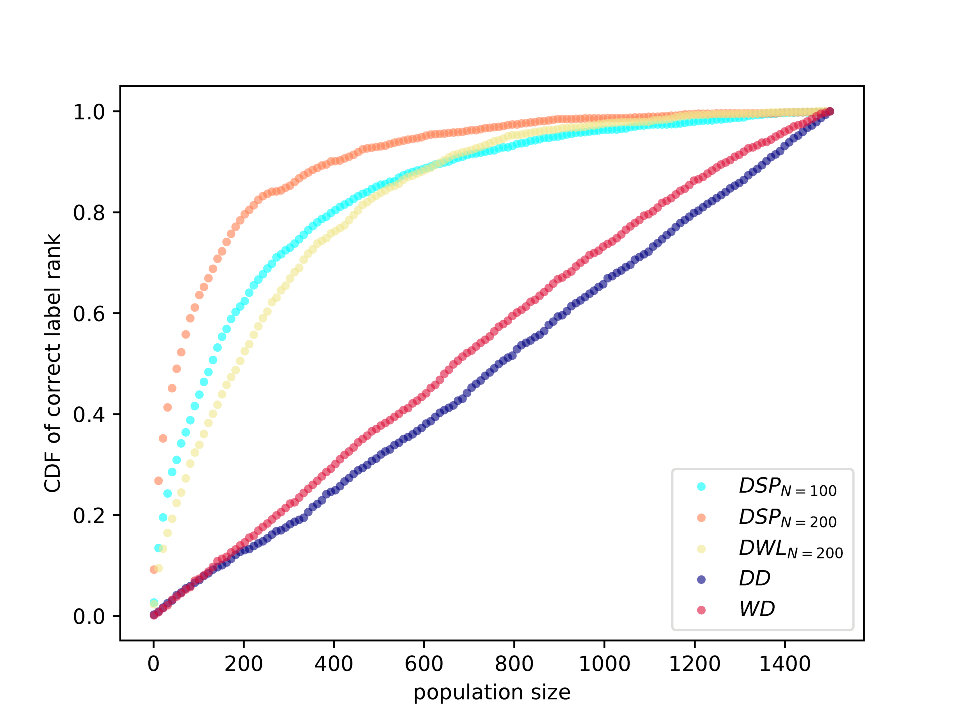
\includegraphics[width=0.8\linewidth]{\MyPath/fig/kernels_evaluation.pdf}
	\caption{\emph{CDF} of true rank over the population according to different kernels.}
	\label{fig:kernels_evaluation}
\end{figure}

The best overall performance is achieved by the \emph{DSP} kernel on graphs pruned to $ 200 $ nodes.
In particular, this kernel places the true identity among the closest 10 networks for $10\%$ of the individuals, and among the closest $ 200 $ networks for $ 80\%$ of the population.
The Shortest-Path kernel has an intuitive interpretation in the case of mobility networks, since its atomic substructures take into account the hop distances among the locations in a user's mobility network and the popularity categories of the departing and arrival locations.
The deep variant can also account for variation at the level of such substructures, which are more realistic when considering the stochasticity in the mobility patterns inherent to our dataset.

The best performance of the Weisfeiler-Lehman kernel is achieved by its deep variant for $ h=2 $ iterations of the \emph{WL} test for a mobility network pruned to $200$ nodes.
This phenomenon is explainable via the statistical properties of the mobility networks.
As we saw in~\cref{sec:data-stats}, the networks display power law degree distribution and small diameters.
Taking into account the steps of the \emph{WL} test, it is clear that these topological properties will lead the node relabeling scheme to cover the entire network after a very small number of iterations.
Thus local structural patterns will be described by few features produced in the first iterations of the test.
Furthermore, the feature space of the kernel increases very quickly as a function of $ h $, which leads to sparsity and low levels of similarity over the population of networks.

Histograms of length $10^3$ were also computed for the unweighted and weighted degree distributions and passed through a Gaussian RBF kernel.
We can see that the unweighted degree distribution \emph{DD} gives almost a random ranking, as this kernel produces a very high-dimensional mapping, which is heavily dependent on the network size. When including the normalized edge weights, the \emph{WD} kernel only barely outperforms a random ranking.
Repetitions on pruned versions, which partly mitigate dimensionality effects, did not significantly improve the performance and are not presented for brevity.

Based on the insights obtained from our experiment, we can make the following observations with respect to attributes of individual mobility and their impact on the identifiability of networks:
%




\begin{itemize}

	\item \textbf{Transition pruning}: Including very rare transitions in longitudinal mobility does not add discriminative information.
	We consistently obtained better results when truncating the long tail of edge weight distribution, which led us to analyze versions of the networks where $40\%$ of the weakest edges were removed.
	\item \textbf{Frequency information of locations}: The frequency of visits to nodes in the mobility network allows better ranking by kernels which support node attributes, e.g.\ the Weisfeiler-Lehman and the Shortest-Path kernel.
	This information should follow a coarse scheme, in order to compensate for the temporal variation of location popularity in mobility networks.
	\item \textbf{Directionality of transitions}: Directionality generally enhances the identifiability of networks and guides the similarity computation when using Shortest-Path kernels.
\end{itemize}

\subsection{Quantification of privay loss}

\begin{figure}[!t]
	\centering
	\begin{minipage}[b]{.45\textwidth}
		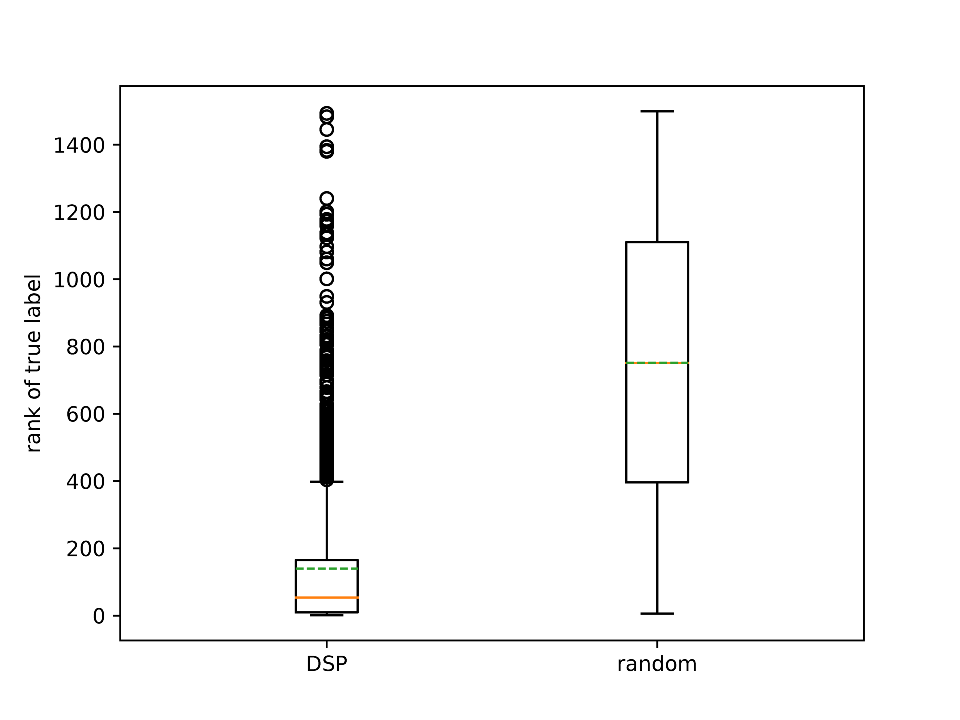
\includegraphics[width=1.2\linewidth]{\MyPath/fig/rank_correct_.pdf}
		\caption{{Boxplot of rank for the true labels of the population according to a Deep Shortest-Path kernel and to a random ordering.}}
		\label{fig:rank_correct}
	\end{minipage}\qquad
	\begin{minipage}[b]{.45\textwidth}
		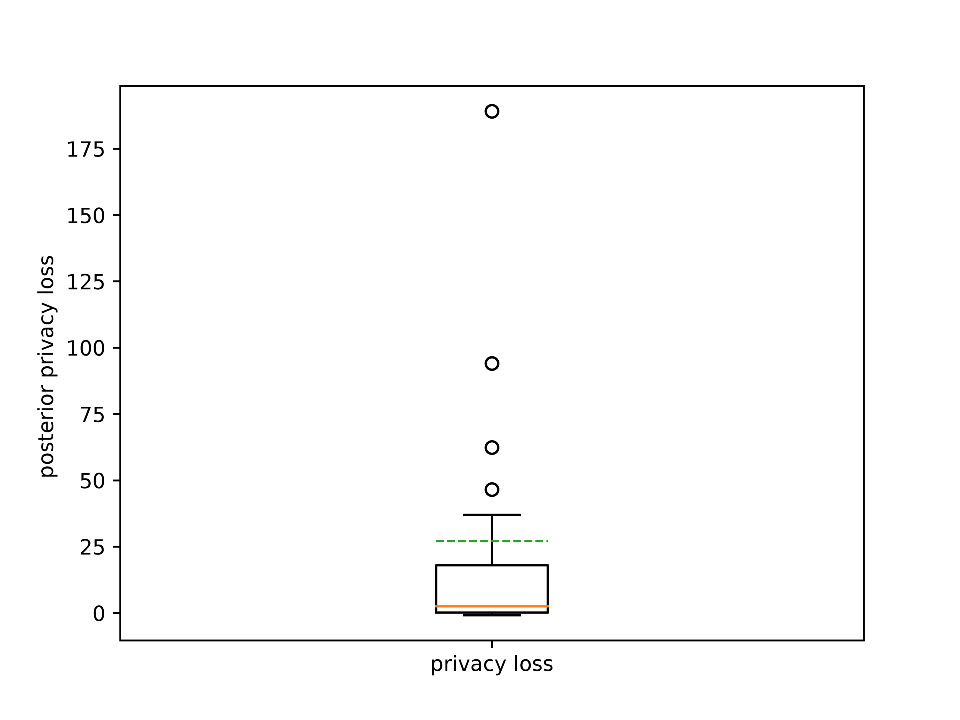
\includegraphics[width=1.2\linewidth]{\MyPath/fig/posterior_privloss_.pdf}
		\centering \caption{{Privacy loss over the test data of our population for an adversary adopting the informed policy of~\eqref{eq:inverse_rank}. Median privacy loss is 2.52.}}
		\label{fig:privloss}
	\end{minipage}
\end{figure}

The Deep Shortest-Path kernel on top$-200$ networks offers the best ranking of identities for the test networks.
As observed in~\cref{fig:rank_correct}, the mean of the true rank has been shifted from $ 750 $ to $ 140 $ for our population.
In addition, the variance is much smaller: approximately $ 218 $, instead of $ 423 $ for the random ordering.

The obtained ordering implies a significant decrease in user privacy, since the ranking can be leveraged by an adversary to determine the most likely matches between a training mobility network and a test mobility network.
The adversary can estimate the true identity of a given test network $ G' $, as suggested in~\cref{sec:threat-model}, applying some simple probabilistic policy that uses pairwise similarity information. For example, let us examine the privacy loss implied by the update rule in~\eqref{eq:adversarial_rule} for  \mbox{function $ f$}:

\[
f\left(K_{\text{DSP}}(G_i, G')\right) :=\frac{1}{\text{rank}\left(K_{DSP}(G_i, G')\right)}.
\label{eq:inverse_rank}
\]

This means that the adversary updates her probability estimate for the identity corresponding to a test network, by assigning to each possible identity a probability that is inversely proportional to the rank of the similarity between the test network and the training network corresponding to the identity.

From equation~\eqref{eq:privloss}, we can compute the induced privacy loss for each test network, and the statistics of privacy loss over the networks of the Device Analyzer population.
\cref{fig:privloss} demonstrates considerable privacy loss with a median of $ 2.52 $.
This means that the informed adversary can achieve a median deanonymization probability $3.52$ times higher than an uninformed adversary.
Moreover, the positive mean of privacy loss ($ {\approx  27}$) means that the probabilities of  the true identities of the test networks have, on average, much higher values in the adversarial estimate compared to the uninformed random strategy.
Hence, revealing the kernel values makes an adversarial attack easier.

\subsection{Defense mechanisms }

The demonstrated privacy leakage motivates the quest
for defense mechanisms against this category of attacks.
There are a variety of techniques which we could apply in order to \emph{reduce the recurring patterns of an individual's mobility network over time} and \emph{decrease the diversity of mobility networks across a population}, therefore enhancing the privacy inherent in these graphs.
Examples include noise injection on network structure via several strategies: randomization of node attributes, perturbations of network edges, or node removal.
It is currently unclear how effective such techniques will be, and what trade-off can be achieved between utility in mobility networks and the privacy guarantees offered to individuals whose data the graphs represent.
Moreover, it seems appropriate to devise kernel-agnostic techniques, suitable for generic defense mechanisms.
For example, it is of interest to assess the resistance of our best similarity metric to noise, as the main purpose of deep graph kernels is to be robust to small dissimilarities at the substructure level.

We think this study is important for one further reason: kernel-based methods allow us to apply a rich toolbox
of learning algorithms without accessing the original datapoints, or their feature vectors, but instead by querying their kernel matrix.
Thus studying the anonymity associated with kernels is valuable for ensuring that such learning systems do not leak the privacy of the original data.

\section{Summary \& discussion} %\& Future Work}

In this chapter we have shown that the mobility networks of individuals exhibit significant diversity, and the topology of the mobility network itself, without labels, may be unique and therefore uniquely identifying.

An individual's mobility network is dynamic over time.
Therefore, an adversary with access to mobility data of a person from one time period cannot simply test for graph isomorphism to retrieve the same user from a dataset recorded at a different point in time.
Hence we proposed graph kernel methods to detect structural similarities between two mobility networks, and thus provide the adversary with information on the likelihood that two mobility networks represent the same individual.
While graph kernel methods are imperfect predictors, they perform significantly better than a random strategy and therefore our approach induces significant privacy loss.
Our approach does not make use of geographic information or fine-grained temporal information. Therefore, our method is immune to commonly adopted privacy intending practices of geographic information masking or removal, and temporal cloaking, and thus it may lead to new mobility deanonymization attacks.

Moreover, we find that reducing the number of edges~(transitions between locations) in a mobility network does not necessarily make the network more privacy-preserving, while user anonymity is violated even when reducing the number of nodes~(locations).
Conversely, releasing the frequency of node visits and the direction of transitions in a mobility network does aid the identifiablility of a mobility network for adversaries applying graph kernel similarity metrics on identified historical data.
We provide empirical evidence that neighborhood relations in the high-dimensional spaces generated by the tested deep graph kernels remain meaningful for our dataset of networks~\citep{Beyer}.
Further work is needed to shed more light on the geometry of those spaces in order to derive the optimal substructures and dimensionality required to support best graph set matching.
More work is also required to understand the sensitivity of our approach to the time period over which mobility networks are constructed.
There is also an opportunity to explore better ways of exploiting pairwise distance information.

Beyond emphasizing the vulnerability of popular anonymization techniques based on user-specific location pseudonymization, our work provides insights into network features that can facilitate the identifiability of location traces.
Our framework also opens the door to new anonymization techniques that can apply structural similarity methods to individual traces in order to cluster people with similar mobility behaviour.
This approach may then support statistically faithful population mobility studies on mobility networks securing $k-$anonymity guarantees for participants.

Apart from graph kernel similarity metrics, tools for network deanonymization can also be sought in the direction of graph mining: applying heavy subgraph mining techniques~\citep{Bogdanov2011}, or searching for persistent cascades~\citep{Morse16}.
Frequent substructure pattern mining (e.g.~gSpan,~\textcitecustom{Yan2002}) and discriminative frequent subgraph mining (e.g.~CORK,~\textcitecustom{Thoma2010}) techniques can also be considered.

Our methodology is, in principle, applicable to all types of data where individuals transition amongst a set of discrete states.
Therefore, the performance of such retrieval strategies can also be evaluated on different categories of datasets, such as web browsing histories, or smartphone application usage sequences.

A drawback of our current approach is that it cannot be directly used to mimic individual or group mobility by synthesizing traces.
Fitting a generative model on mobility traces and then defining a kernel on this model~\citep{song11} may provide better anonymity, and therefore privacy, and it would also support the generation of artificial traces which mimic the mobility of users.


\chapter{Bayesian Pseudocoresets}
\label{chap:chap4}
\renewcommand*{\MyPath}{../Chapter4}%
In~\cref{chap:chap2}, we exposed the prohibitive computational limitations of Bayesian inference in the regime of modern large-scale data, and discussed coreset-based summarization as a viable solution for scalable approximate inference under statistical guarantees. In~\cref{chap:chap3}, we considered a case study on a massive high-dimensional dataset capturing longitudinal mobility information of a population, and quantified the privacy loss incurred via coarse representations of the datapoints for fast analysis.
Motivated by the quest for scalable learning methods on sensitive data, in this chapter we propose \emph{Pseudocoresets Sparse Variational Inference}, a general-purpose approximate inference method designed to enable scalable inference on high-dimensional datasets, under the guarantees of approximate differential privacy.

We begin by investigating the shortcomings of existing Bayesian coreset constructions 
in the increasingly common setting of sensitive, high-dimensional data. 
In particular, we prove that there are situations in which 
the Kullback-Leibler divergence between the \emph{optimal} coreset 
and the true posterior grows with data dimension; and as coresets include
a subset of the original data, they cannot be constructed in a manner
that preserves individual privacy.
We address both of these issues with a single unified solution, \emph{Bayesian
pseudocoresets}---a small weighted collection of synthetic
``pseudodata''---along with a variational optimization method to select both
pseudodata and weights.  The use of pseudodata (as opposed to
the original datapoints) enables both the summarization of high-dimensional data
and the  differentially private summarization of
sensitive data. Real and
synthetic experiments on high-dimensional data demonstrate that Bayesian 
pseudocoresets achieve significant improvements in posterior approximation error compared to
traditional coresets, and that pseudocoresets provide privacy without
a significant loss in approximation quality. 


%This chapter is based on~\citep{psvi}.
\section{Related work \& contributions}
\label{sec:intro}

Large-scale data---which has become the norm in many scientific and commercial applications of statistical machine learning---creates
an inherently difficult setting for the modern data analyst. Exploring such data is difficult because it cannot all be
obtained and directly visualized at once; one is typically limited to accessing potentially nonrepresentative random subsets of data.
Exploring models is similarly hard, as training even a single model can be a computationally expensive, slow, and unreliable process.
And as many sources of large-scale data contain sensitive information about 
individuals (e.g., electronic health records and social network data),
these challenges are coupled with growing privacy concerns  that preclude direct access to individual datapoints completely. 

Large-scale data does offer one reprieve to the analyst: it often exhibits a significant degree of redundancy. Most datapoints are 
not unique or particularly informative for modeling and exploration. Based on this notion, data summarization methods have been developed  
that provide the practitioner with a compressed---but still statistically representative---version of the large dataset for analysis.
Summarizations have been developed for a variety of purposes, e.g., reducing the cost of computing with kernel matrices via Nystr{\"o}m-type approximations~\citep{drineas05,musco17,agrawal19} or sparse pseudo-input parameterizations for Gaussian processes~\citep{williams01,csato02,snelson05,titsias09},
Bayesian inference \citep{huggins16,huggins17,campbell18,campbell19jmlr}, maximum likelihood 
parameter estimation \citep{dumouchel99,madigan02}, 
linear regression \citep{zhou08,guhaniyogi15},
geometric shape approximation \citep{agarwal05},
clustering \citep{feldman11,lucic16,bachem15,braverman16}, and dimensionality reduction \citep{feldman16}.

A common form of summarization is that of a sparse, weighted subset of the original dataset---a \emph{coreset} \citep{agarwal05}. 
Coresets have two distinct advantages over other possible summarization modalities: they are easily interpreted, and can often be used
as the input to standard data analysis algorithms without modification. 
But as the dimensionality of a dataset grows, its constituent 
datapoints tend to become more ``unique'' and cannot represent one another well. Indeed, in the context of Bayesian inference we show that the \emph{optimal} coreset posterior approximation to the true posterior has KL divergence that scales with the dimension 
of the data in a simple problem setting (\cref{prop:original_coreset_fails}). 
Furthermore, directly releasing a subset of the original data precludes any possibility of
individual privacy under the current standard 
of differential privacy \citep{dwork2006calibrating,dwork14}. Past work
addresses this issue in the context of clustering and computational geometry \citep{feldman09,feldman17}---with
the remarkable property that the privatized coreset may be queried \emph{ad infinitum} without
loss of privacy---but no such method exists for Bayesian posterior inference.

In this chapter, we develop a novel technique for data summarization in the context of Bayesian inference, under the constraints that the method is scalable and easy to use, creates an intuitive summarization, applies to high-dimensional data, and enables privacy control. Inspired by past work \citep{madigan02,zhou08,snelson05,titsias09}, instead of using constituent datapoints, we use synthetic \emph{pseudodata} to summarize the large dataset, resulting in a \emph{pseudocoreset}. We show that in the high-dimensional problem setting of \cref{prop:original_coreset_fails}, 
the optimal pseudocoreset with just one pseudodata point recovers the exact posterior, a significant improvement upon the optimal standard coreset of any size.
As in past work on Bayesian coresets \citep{campbell19neurips}, we formulate pseudocoreset construction as variational inference, 
and provide a stochastic optimization method~(\cref{sec:pseudocoresets}). As a consequence of the use of pseudodata---as well as privacy-preserving 
stochastic gradient descent mechanisms~\citep{abadi16,park16, jalko17}---we show that our method can easily be modified to output
a privatized pseudocoreset. The chapter concludes with experimental results demonstrating the performance of pseudocoresets on 
real and synthetic data~(\cref{sec:experiments}).

\section{Bayesian Coresets}
\label{sec:bayesian-coresets}

In this work, the goal is to approximate expectations under a density $\pi(\theta)$, 
 \mbox{$ \theta \in \Theta $} expressed as the product of $N$ potentials 
$ (f(x_n, \theta))_{n=1}^{N} $ and a base density $ \pi_0(\theta)$:
\[
\pi(\theta) &\defined \frac{1}{Z} \exp \left(\sum_{n=1}^{N} f(x_n, \theta)\right) \pi_0(\theta).\label{eq:posterior}
\]
In the setting of Bayesian inference with conditionally independent data, 
the potentials are data log-likelihoods, \ie $f(x_n, \theta) := \log p(x_n | \theta)$,
 $\pi_0$ is the prior density, $\pi$ is the posterior, 
and $Z$ is the marginal likelihood of the data. 
Rather than working directly with $\pi(\theta)$ for 
posterior inference---which requires a $\Theta(N)$ computation per evaluation---a
Bayesian coreset approximation of the form
\[
\pi_w(\theta) \defined \frac{1}{Z(w)} \exp\left(\sum_{n=1}^N w_n f(x_n, \theta)\right)\pi_0(\theta)
\]
for $w\in\reals^N$, $w\geq 0$ may be used in most popular posterior inference schemes \citep{neal11,kucukelbir17,ranganath14}.
If the number of nonzero entries $\|w\|_0$ of $w$ is small, this results in a significant reduction in computational burden.
Recent work has formulated the problem of constructing a  Bayesian coreset of size $M\in\nats$ as sparse variational inference~\citep{campbell19neurips},
\[
& w^\star = \argmin_{w\in\reals^N} \kl{\pi_w}{\pi_1}\label{eq:coresets-vi} \quad \quad
 \text{s.t.} \quad w \geq 0, \; \|w\|_0 \leq M,
\]
and showed that the objective can be minimized using stochastic estimates of $\nabla_w\kl{\pi_w}{\pi_1}$
based on samples from the coreset posterior $\pi_w$. 

\subsection{High-dimensional data}
\label{sec:high_dimensional_data}


Coresets, as formulated in~\cref{eq:coresets-vi}, are limited to using the
original datapoints themselves to summarize the whole dataset.
\cref{prop:original_coreset_fails} shows that this is problematic when
summarizing high-dimensional data; in the common setting of posterior inference
for a Gaussian mean, the KL divergence $\kl{\pi_{w^\star}}{\pi_1}$ of the
\emph{optimal} coreset of any size scales with the dimension of the data.  The
proof may be found in~\cref{app:proofs-of-failure}.
\bnprop \label{prop:original_coreset_fails}
Suppose we use $(X_n)_{n=1}^N \distiid \distNorm(0, I)$ in $\reals^d$ to perform posterior inference in a Bayesian model
with prior 
$\mu \dist \distNorm(0, I)$ and likelihood
$(X_n)_{n=1}^N  \distiid \distNorm(\mu, I).$
Then $\forall M < d$ and $\delta \in[0, 1]$, 
with probability at least $1-\delta$ the optimal size-$M$ coreset $w^\star$ satisfies
\[
\kl{\pi_{w^\star}}{\pi_1} \geq \frac{1}{2}\frac{N-M}{1+N}F_{d-M}^{-1}\left(\delta{N\choose M}^{-1}\right),
\]
where $F_{k}$ is the CDF of a $\chi^2$ random variable with $k$ degrees of freedom.
\enprop

The bound in \cref{prop:original_coreset_fails} depends on $d$ through the
$\chi^2$ distribution inverse CDF. Although difficult to see directly, the
bound is reasonably large for typical values of $N, M, d, \delta$, and
increasing linearly in $d$; \cref{fig:klbound} visualizes the value of the
lower bound as a function of dimension $d$ for various coreset sizes $M$. Note
that the above bound requires the data to be high-dimensional such that $d >
M$; if $d\leq M$ the proof technique used above results in a vacuous
$\kl{\pi_{w^\star}}{\pi_1} = 0$ lower bound. 

\captionsetup[subfigure]{labelformat=empty}
\begin{figure}[t!]
	\centering 
\begin{subfigure}[b]{.45\textwidth} 
	\scalebox{1}{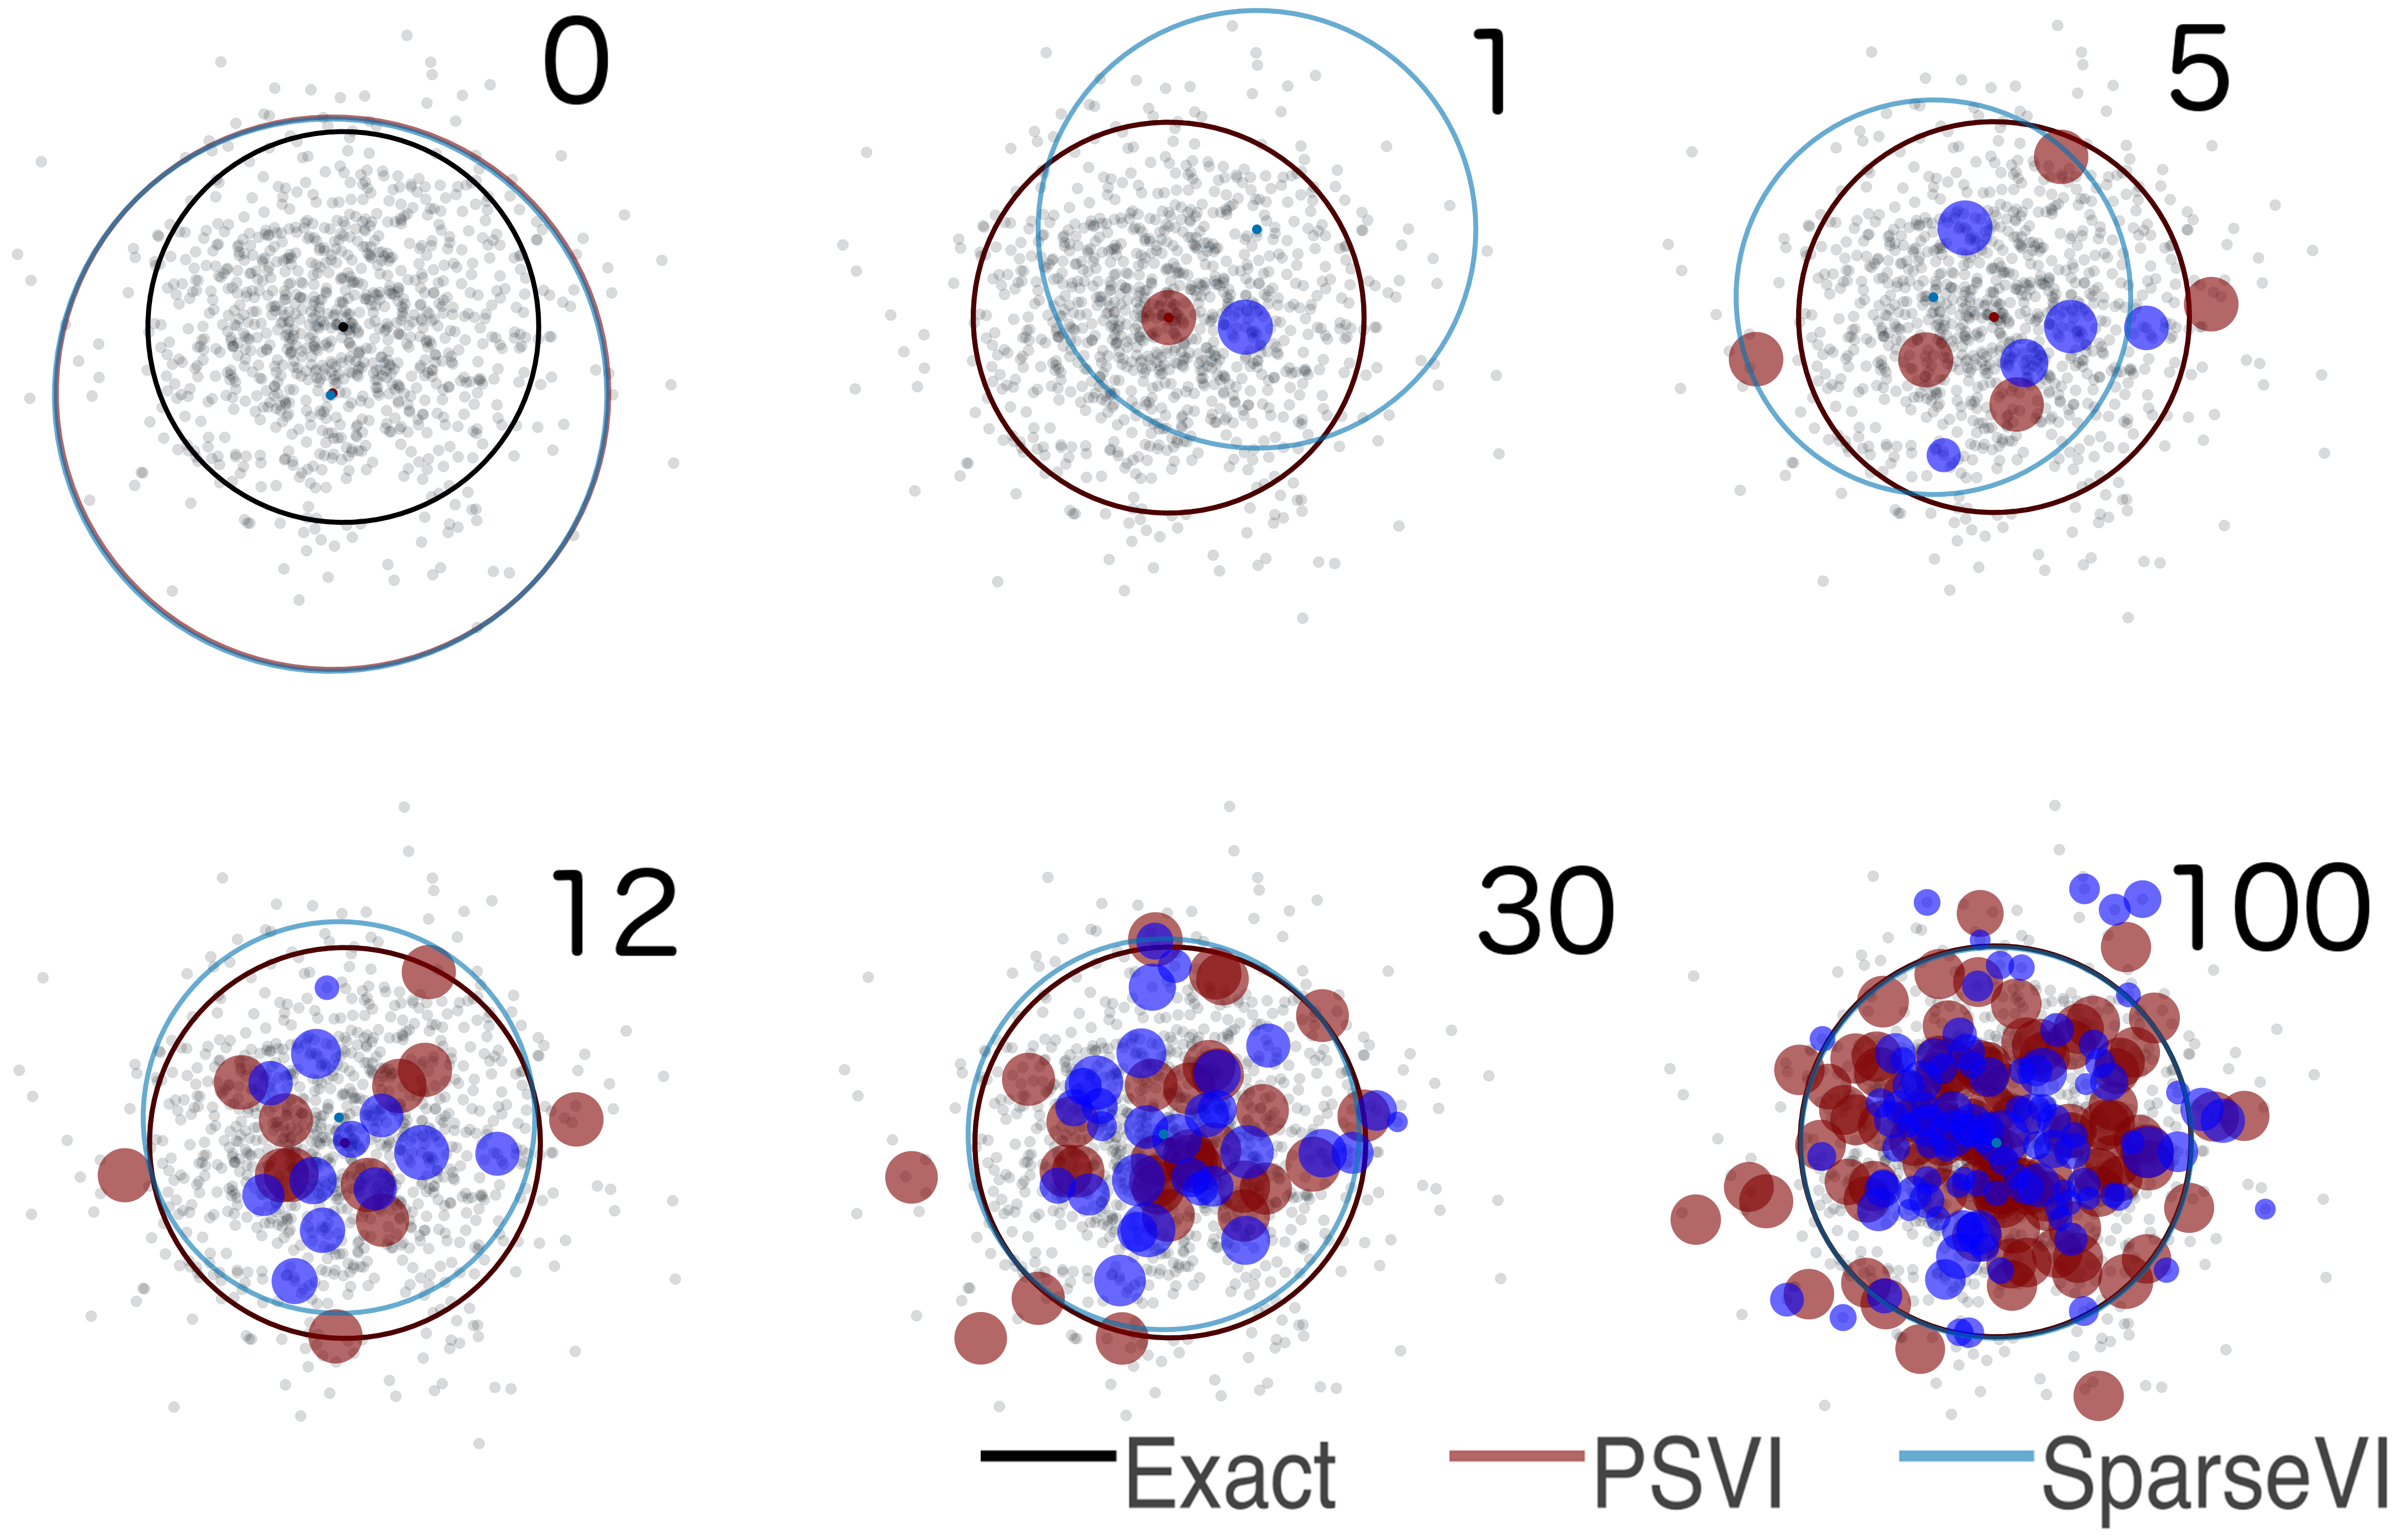
\includegraphics[width=\textwidth]{\MyPath/figs/d500_pts_combined.png}}
	\caption{(a)\label{fig:gaussian_coreset_points}}
	\end{subfigure}
\hfill\qquad
\centering
\begin{subfigure}[b]{0.45\textwidth}
	\scalebox{1}{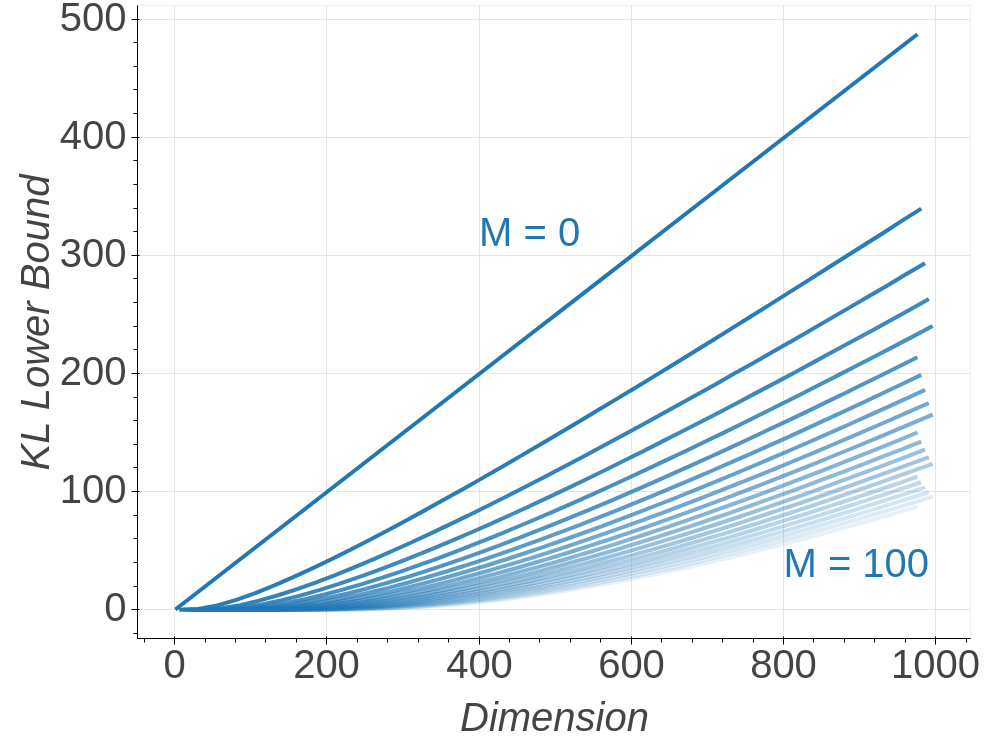
\includegraphics[width=\textwidth]{\MyPath/figs/klbound.png}}
	\caption{(b)\label{fig:klbound}}
\end{subfigure}
\caption{Gaussian mean inference under~pseudocoreset (\psvi)~against~standard coreset (\sparsevi) summarization for $N=1,000$  datapoints. (\subref{fig:gaussian_coreset_points})~Progression of~\psvi~vs.~\sparsevi~construction for coreset sizes $M=0, 1, 5, 12, 30, 100$, in 500 dimensions~(displayed are datapoint projections on 2 random dimensions).~\psvi~and~\sparsevi~coreset predictive $3\sigma$ ellipses are displayed in red and blue respectively, while the true posterior $3\sigma$ ellipse is shown in black.~\psvi~has the ability to immediately move pseudopoints towards the  true posterior mean, while \sparsevi~has to add a larger number of existing points in order to obtain a good posterior approximation. See \cref{fig:gaussian_dkl} for the quantitative KL comparison.
(\subref{fig:klbound})~Optimal coreset KL divergence lower bound from \cref{prop:original_coreset_fails} as a function of dimension with $\delta = 0.5$, and  coreset size $M$ evenly spaced from 0 to 100 in increments of 5.}
\end{figure}


\section{Bayesian Pseudocoresets}
\label{sec:pseudocoresets}

\Cref{prop:original_coreset_fails} shows that there is room 
for improvement in coreset construction in the high-dimensional data regime.
Indeed, consider again the same problem setting; the coreset posterior distribution
is a Gaussian with mean $\mu_w$ and covariance $\Sigma_w$,
\[
\Sigma_w &=\left(1+\sum_{n=1}^N w_n\right)^{-1} I & \mu_w &= \Sigma_w \sum_{n=1}^N w_n X_n.\label{eq:gausswpost}
\]
Examining \cref{eq:gausswpost}, we can replicate any coreset posterior exactly by using a single synthetic \emph{pseudodata} point $U = \left(\sum_{n=1}^Nw_n\right)^{-1}\sum_{n=1}^N w_nX_n$
with weight $\sum_{n=1}^N w_n$. In particular, the true posterior is equivalent to the posterior
conditioned on the single pseudodata point $U = \frac{1}{N}\sum_{n=1}^N X_n$ with weight $N$ (with corresponding KL divergence equal to 0).
This is not surprising; the mean of the data is precisely a sufficient statistic for the data in this 
simple setting. However, it does illustrate that carefully-chosen pseudodata may be able to
represent the overall dataset---as ``approximate sufficient statistics''---far better than any reasonably small collection of the original data.
This intuition has been used before, e.g., for scalable Gaussian process inference \citep{snelson05,titsias09},
privacy-preserving compression in linear regression \citep{zhou08}, herding~\citep{welling09, chen10, huszar12}, and deep generative models~\citep{tomczak18}.

In this section, we extend the 
realm of applicability of pseudopoint compression methods to the general class of Bayesian posterior 
inference problems with conditionally independent data, resulting in \emph{Bayesian pseudocoresets}.
Building on recent work \citep{campbell19neurips}, we formulate pseudocoreset construction 
as a variational inference problem where both 
the weights and pseudopoint locations are parameters of the variational posterior approximation,
and develop a stochastic algorithm to solve the optimization. 

\subsection{Pseudocoreset variational inference}\label{sec:pseudovi}
A Bayesian pseudocoreset takes the form
\[
 \pi_{u,w}(\theta) = \frac{1}{Z(u, w)} \exp \left( \sum_{m=1}^{M} w_m f(u_m,\theta) \right) \pi_0(\theta),
\label{eq:pseudo-posterior}
\]
where $u\defined (u_m)_{m=1}^M$ are $M$ pseudodata points $u_m\in\reals^d$, $(w_m)_{m=1}^M$ are nonnegative weights,
$f : \reals^d \times \Theta \to \reals$ is a potential function parametrized by a pseudodata point,
and $Z(u, w)$ is the corresponding normalization constant rendering $\pi_{u, w}$ a probability density. In the setting of Bayesian posterior inference,
$u_m$ will take the same form as the data, while the potentials are the log-likelihood functions, i.e., $f(u_m, \theta) = \log p(u_m | \theta)$.
We construct a coreset by minimizing the KL divergence over both the pseudodata locations and weights, 
\[
u^\star, w^\star = \argmin_{\substack{u\in\reals^{d \times M}}, w\in\reals^M_+}\,\, \kl{\pi_{u,w}}{\pi}. 
\label{eq:pseudo-coreset-vi}
\]
As opposed to previous Bayesian coreset construction optimization problems~\citep{campbell18, campbell19jmlr, campbell19neurips}, 
we do not need an explicit sparsity constraint; the coreset size is limited to $M$ directly through the selection of the number
of pseudodata and weights. 

Denote the vectors of original data potentials $f(\theta)\in\reals^N$ and synthetic pseudodata potentials ${\tf(\theta)\in\reals^M}$ as
$
f(\theta) \defined \left[
f_1(\theta)
\ldots
f_N(\theta)
\right]^T
$
and
$
\tf(\theta) \defined \left[
f(u_1,\theta)
\ldots
f(u_M,\theta)
\right]^T
$ 
respectively,
where we suppress the $(\theta)$ for brevity where clear from context. 
Denote $\EE_{u,w}$ and $\cov_{u,w}$ to be the expectation and covariance operator for the pseudocoreset posterior $\pi_{u,w}$.
Then we may write the KL divergence in \cref{eq:pseudo-coreset-vi}  as
\[
  \kl{\pi_{u,w}}{\pi} = &\EE_{u,w}[\log \pi_{u,w}(\theta)] - \EE_{u,w}[\log \pi(\theta)] \\
 = &\log Z(1) - \log Z(u, w)
- 1^T\EE_{u,w} [f] +  w^T\EE_{u,w} [\tf],
\label{eq:kl-expanded}
\]
where $1\in\reals^N$ is the vector of all 1 entries, and $w\in\reals^M$ is the vector of pseudocoreset weights.

As we will employ gradient descent steps as part of our algorithm to minimize the variational objective over the parameters $u, w$,
we need to evaluate the derivative of the KL divergence \cref{eq:kl-expanded}. Despite the presence of the 
intractable normalization constants and expectations, we show in \cref{supp:gradient_derivations}
that gradients can be expressed using moments of the pseudodata and original data potential vectors.
In particular, 
the gradients of the KL divergence with respect to the weights $ w$ and to a single pseudodata location $u_m$ are 
\[
& \nabla_w\mathrm{D}_{\mathrm{KL}} = - \cov_{u,w}[\tf ,f^T1 - \tf^Tw], \,\,
&\nabla_{u_m}\mathrm{D}_{\mathrm{KL}} = -w_m\cov_{u,w}\left[h(u_m), f^T1 - \tf^Tw\right],
\label{eq:dkl_duw}
\]
where $h(\cdot, \theta) \defined \nabla_u f(\cdot, \theta)$, and the $\theta$ argument is again suppressed for brevity.






\subsection{Stochastic optimization}\label{sec:stochopt}


The gradients in \cref{eq:dkl_duw} involve expectations of (gradient) log-likelihoods from the model.
Although there are a few particular Bayesian models where these can be evaluated in closed-form
(e.g.~the synthetic experiment in \cref{section:gaussian_experiment}; see also \cref{supp:gaussian_experiment_appendix}),
this is not usually the case. In order to make the proposed pseudocoreset method broadly applicable,
in this section we develop a black-box stochastic optimization scheme (\cref{alg:psvi}) for \cref{eq:pseudo-coreset-vi}. 


\algnewcommand{\IfThenElse}[3]{% \IfThenElse{<if>}{<then>}{<else>}
	\State \algorithmicif\ #1\ \algorithmicthen\ #2\ \algorithmicelse\ #3}
\algrenewcommand{\algorithmiccomment}[1]{\hfill #1}
%\algrenewcommand{\algorithmiccomment}[1]{\hfill$\triangleright$ #1}
\newcommand{\Commenttriangle}[1]{\algorithmiccomment{\hfill$\triangleright$ #1}}

\setlength{\textfloatsep}{10pt}% Remove \textfloatsep

\begin{algorithm}[!ht]
	\caption{Pseudocoreset Variational Inference}
	\label{alg:psvi}
	\begin{algorithmic}[1]
		\Procedure{PSVI}{$f(\cdot, \cdot), \pi_0, x, M, B, S, T, (\gamma_t)_{t=1}^{\infty}$}
		\LineCommentIndent{Initialize the pseudocoreset using a uniformly chosen subset of the full dataset}
		\State $N \gets $ \# datapoints in $x, \quad \mcB\dist\distUnifSubset\left([N], M\right), \quad \mcB \defined \left\{b_1, \dots, b_M\right\}$ 
		\State $u_m \gets x_{b_m}, \quad w_m \gets \nicefrac{N}{M}, \quad m=1, \dots, M$
		\For{$ t = 1, \ldots, T$}
		\LineCommentIndent{\mbox{Take $S$ samples from current pseudocoreset posterior}}
		\State $(\theta)_{s=1}^{S}  \distiid \pi_{u,w}$ where $\pi_{u,w}(\theta) \propto \exp\left(\sum_{m=1}^Mw_m f(u_m, \theta)\right)\pi_0(\theta)$
		\State $\mcB\dist\distUnifSubset\left([N], B\right)$ \Commenttriangle{\mbox{Obtain a minibatch of $B$ points from the full dataset}}
		\For{$s = 1, \dots, S$} 	\Commenttriangle{\mbox{Compute (gradient) log-likelihood discretizations}}
		\State $g_{s} \gets \left( f(x_b, \theta_s ) - \nicefrac{1}{S}\sum_{s'=1}^S f(x_b, \theta_{s'}) \right)_{b\in\mcB} \in \reals^B$ 
		\State $\tg_s\gets \left(f(u_m, \theta_s) - \nicefrac{1}{S}\sum_{s'=1}^S f(u_m, \theta_{s'})\right)_{m=1}^M\in\reals^M$
		\For{$m = 1, \dots, M$}
		\State $\tildeh_{m,s} \gets \nabla_u f(u_m, \theta_s) - \nicefrac{1}{S}\sum_{s'=1}^S \nabla_u f(u_m, \theta_{s'})\in\reals^d$
		\EndFor
		\EndFor
		\State $\hat\nabla_w \gets -\nicefrac{1}{S}\sum_{s=1}^S \tg_s\left(\nicefrac{N}{B} g_s^T1 - \tg_s^Tw\right)$\Commenttriangle{\mbox{Compute Monte-Carlo gradients for $w$}}
		\For{$m = 1,\dots, M$}
		\Comment{and $(u_m)_{m=1}^M$}
		\State $\hat\nabla_{u_m} \gets -w_m\nicefrac{1}{S}\sum_{s=1}^S \tildeh_{m,s}\left(\nicefrac{N}{B} g_s^T1 - \tg_s^Tw\right)$
		\EndFor
		\State $w \gets \max(w - \gamma_t\hat\nabla_w, 0)$ \Commenttriangle{\mbox{Take stochastic gradient step in $w$}}
		\For{$m = 1,\dots, M$} \Comment{and $(u_m)_{m=1}^M$}
		\State $u_m \gets u_m - \gamma_t\hat\nabla_{u_m}$
		\EndFor
		\EndFor
		\State\Return $w$, $(u_m)_{m=1}^M$
		\EndProcedure		 
	\end{algorithmic}
\end{algorithm}



To initialize the pseudocoreset, we subsample $M$ datapoints from the large dataset and reweight them
to match the overall weight of the full dataset,
\[
&u_m \gets x_{b_m}, \quad w_m \gets N/M, \quad m=1, \dots, M\\
&\mcB\dist\distUnifSubset\left([N], M\right), \quad \mcB \defined \left\{b_1, \dots, b_M\right\}. 
\]

After initializing the pseudodata locations and weights,
we simultaneously optimize \cref{eq:pseudo-coreset-vi} over both.
Each optimization iteration $t\in \{1, \dots, T\}$ consists of a stochastic gradient descent step
with a learning rate $\gamma_t \propto t^{-1}$,  
\[
w_m \gets \max\left(0, w_m - \gamma_t (\hat\nabla_{w})_m\right),
\quad u_m \gets u_{m} - \gamma_t \hat\nabla_{u_{m}},
\quad 1\leq m \leq M.
\label{eq:gd-update}
\]
The stochastic gradient estimates $\hat\nabla_w \in \reals^M$ and $\hat\nabla_{u_m} \in \reals^d$
are based on $S\in\nats$ samples $\theta_s \distiid \pi_{u,w}$ from the coreset approximation
and a minibatch of $B\in\nats$ datapoints from the full dataset,
\[
\hat\nabla_w \defined -\frac{1}{S}\sum_{s=1}^{S} \tg_s \left(\frac{N}{B}g_s^T 1  -  \tg_s^Tw  \right) \label{eq:weight-optimization-mc}, \quad \\
 \hat\nabla_{u_m} \defined - w_m \frac{1}{S}\sum_{s=1}^{S} \tildeh_{m,s}  \left(\frac{N}{B}g_s^T 1 - \tg_s^T w \right), \label{eq:location-optimization-mc-cov}
\]
where
\[
\begin{aligned}
& \tildeh_{m,s} \defined\nabla_u f(u_m, \theta_s) - \frac{1}{S} \sum_{s'=1}^{S}\nabla_u f(u_m, \theta_{s'}),
\quad & g_s \defined \left. \left(f(\theta_s) - \frac{1}{S} \sum_{s'=1}^{S} f(\theta_{s'})\right)\right|_{\mcB}\\
& \tg_s \defined \tf(\theta_s) - \frac{1}{S} \sum_{s'=1}^{S} \tf(\theta_{s'}),
\quad & \mcB \dist \distUnifSubset\left([N], B\right),
\end{aligned}\label{eq:gradparts}
\] 
and $\left.(\cdot)\right|_{\mcB}$ denotes restriction of a vector to only those indices in $\mcB\subset[N]$.
Crucially, note that this computation does not scale with $N$, but rather with the number
of coreset points $M$, the sample and minibatch sizes $S$ and $B$, and the dimension $d$.
Obtaining $\theta_s\distiid \pi_{u,w}$ efficiently via Markov chain Monte Carlo sampling
algorithms~\citep{hoffman14,jacob17} is (roughly) $O(M)$ per sample, because the coreset is always of size $M$;
and we need not compute
the entire vector $g_s\in\reals^N$ per sample $s$, but rather only those $B\ll N$ indices in the minibatch $\mcB$,
resulting in a cost of $O(B)$.
Aside from that, all computations involving $\tg_s\in\reals^M$ and $\tildeh_{m,s}\in\reals^d$ are at most $O(Md)$.
Each of these computations are repeated $S$ times over the coreset posterior samples.












\subsection{Differentially private scheme}
\label{sec:dp-pseudocoresets}

Beyond better summarizations of high-dimensional data, pseudocoresets enable the 
generation of a data summarization that ensures the statistical privacy of individual datapoints under the model of (approximate) \emph{differential privacy}. In this setting, a trusted
 curator holds an aggregate dataset of $N$ datapoints, $x\in\mcX^N$, $\mcX\subseteq \reals^d$, and 
builds and releases a pseudocoreset $(u, w)$, $u\in\mcX^M$, $w\in\reals_+^M$ via
a randomized mechanism satisfying \cref{def:dp-definition}~\citep{dwork06, ourdata}.
\ndefn[($\veps, \delta$)-Differentially Private Coreset]{
	Fix $\veps \geq 0, \delta \in [0,1]$. A pseudocoreset construction algorithm
        $ \mcM: \mcX^N \rightarrow \reals_+^M\times\mcX^M $  is  ($\veps, \delta$)-differentially private if for every pair of 
        adjacent datasets $ x \approx x'$ and all events $ A \subseteq \reals_+^M\times\mcX^M$, 
	$\;\Pr[\mcM(x) \in A] \leq e^\veps \Pr[\mcM(x') \in A] + \delta$.
	\label{def:dp-definition}
}

As in~\cref{sec:bdp}, we consider two datasets $x, x'$ as adjacent (denoted 
$ x \approx x' $) if $ x' $ can be obtained from $ x $ by adding or removing an
element.  $ \veps $ controls the effect that removal or addition of an element
can have on the output distribution of $\mcM$, while %additive term 
$ \delta $
captures the failure probability, 
%that plain \mbox{$\veps$-differential} privacy is
%allowed to be broken, 
and is preferably $ o(1/N)$. 

In this section, we develop a differentially private version of pseudocoreset construction.
Beyond modifying our initialization scheme, private pseudocoreset
construction comes as natural extension of \cref{alg:psvi}
 via replacing gradient computation involving points of the
true dataset with its differentially private counterpart. 


\subsubsection{Pseudodata points initialization}
\label{sec:pseudo-points-initilization}

In the standard (nonprivate) pseudocoreset construction (\cref{alg:psvi}), pseudopoints are initialized from the dataset itself,
incurring a privacy penalty. In differentially private pseudocoreset construction,
we simply initialize pseudopoints by generating synthetic data from the statistical model
at no privacy cost.



\subsubsection{Optimization}
\label{sec:private-wu-opt}
Examining lines 4--19 of \cref{alg:psvi}, the only steps that involve
handling the original data occur at lines 8, 12, and 14, 
when we use the minibatch subsample to compute log-likelihoods and gradients. 
Due to the post-processing property of differential privacy~\citep{dwork14},
all of the other computations in \cref{alg:psvi} (e.g.~sampling from the pseudocoreset posterior, 
computing pseudopoint log-likelihoods, etc.) incur no privacy cost.
Therefore, we need only %to modify the gradient estimates 
to control the influence of private data entering  the gradient computation through the vector of $ (g_s^T1)_{s=1}^{S}$ terms.

To accomplish this we do repeated applications of the  \emph{subsampled
Gaussian mechanism}, since this also allows us to use a
\emph{moments accountant} technique
to keep tight estimates of
privacy parameters~\citep{abadi16, wang19}. As in the nonprivate scheme, in
each optimization step we uniformly subsample a minibatch $\mcB = \{x_1, \dots,
x_{B}\}$ of private datapoints. 
We then replace the $g_s^T1$ term in lines 12 and 14
with a randomized privatization:
\begin{align}
& \text{replace}\quad (g_s^T 1)_{s=1}^{S}\quad\text{with}\quad  Z+\sum_{i=1}^{B}{\frac{G_{i}}{\max\left(1,\frac{||G_{i}||_2}{C}\right)}},
&Z \dist \distNorm(0, \sigma^2 C^2 I),\label{eq:dp_suffstats}
\end{align}
where $G_i:=\left( f(x_i, \theta_s) - \frac{1}{S} \sum_{s'=1}^{S} f(x_i, \theta_{s'})\right)_{s=1}^{S} \in \reals^S  \; \forall x_i \in \mcB$,
and $C, \sigma > 0$ are parameters controlling the amount of privacy.
This modification to \cref{alg:psvi} has been shown in past work to obtain the privacy guarantee provided in \cref{cor:dp_sgd_privacy};
crucially, the privacy cost of our construction is independent of the pseudocoreset size.
It also does not introduce any significant amount of additional computation.
No sensitivity computation for privatisation noise calibration is required, as boundedness is 
enforced via clipping in \cref{eq:dp_suffstats}. Finally, a manageable number of privacy specific 
hyperparameters is introduced: the clipping bound $C$ and noise level $\sigma$.
\bncor[\textcite{abadi16}]
 There exist constants $ c_1, c_2 $ such that \cref{alg:psvi} modified per \cref{eq:dp_suffstats} 
is $(\veps, \delta)$-differentially
private for any $ \veps < c_1q^2T$, $ \delta > 0$, and  \mbox{$ \sigma
\geq c_2q \sqrt{T \log(1/\delta)}/\veps$}, where $ {q \defined \frac{B}{N} }$
is the fraction of data in a minibatch and $T$ is the number of optimization
steps. \label{cor:dp_sgd_privacy}
\encor
%\begin{comment}
%gradients per single private datapoint $\tilde\nabla_{w,u}^{(i)}\in\reals^{M\times (D+1)}$
% as follows: 
%\[
%\tilde\nabla_{w,u}^{(i)} \defined  & 
%\left[
%\begin{array}{c} 
%-\frac{1}{S} \sum_{s=1}^{S} \tg_s(g_{s,i} - \tg^T_s w/N), \\ 
%- w \frac{1}{S}\sum_{s=1}^{S} \tildeh_s  \left(g_{s, i} - \tg_s^T w/N \right)
%\end{array} \right], 
% \label{eq:dp_grad_i}
%\]
%where $ g_{s, i} \defined f(x_i, \theta_s) - \frac{1}{S} \sum_{s'=1}^{S} f(x_i, \theta_{s'}) \; \forall x_i \in \mcB$.
%
%Finally, we clip the $2$-norm of each such gradient, and release the
%corresponding average with calibrated additive Gaussian noise:
%\begin{align}
%&\tilde\nabla_{w,u} =  N \left(\frac{1}{B}  \sum_{i=1}^B \left(  \frac{\tilde\nabla_{w,u}^{(i)}}{\max{\left(1,\frac{||\tilde\nabla_{w,u}^{(i)}||_2}{C}\right)}} \right) + Z\right) , &Z \dist \distNorm(0, \sigma^2 C^2 I).\label{eq:dp_grad}
%\end{align}
%\end{comment}

\section{Experimental Results}
\label{sec:experiments}
In this section, we evaluate the posterior approximation quality achieved by
pseudocoreset sparse VI (\psvi) compared against uniform random subsampling~(\uniform), Hilbert
coresets~(\giga~\citep{campbell18}) and \sparsevi~greedy coreset
construction~\citep{campbell19neurips}.  For black-box constructions of \sparsevi~and \psvi~we used $S =
100$ Monte Carlo samples per gradient estimation. For \giga~we used a
100-dimensional random projection from a Gaussian approximate posterior $\hpi$
with  two choices for mean and covariance: one set to the exact
posterior~(\optimal), which is not tractable to obtain in practice and forms an
optimistic estimate of achievable approximation quality; and one with mean and
covariance set to a random point on the interpolant between the prior and the
exact posterior point estimates, and subsequently corrupted with $75\%$
additive relative noise~(\realistic). Notably, Hilbert coresets and
\sparsevi~develop incremental schemes for construction, while \psvi~relies on
batch optimization with random initialization~(\cref{alg:psvi}), and does not
use any information from pseudocoresets of smaller size. An incremental scheme
for \sparsevi~is included in~\cref{app:experiments_appendix}. %Code for the presented experiments is available at~\href{https://github.com/dionman/psvi}{https://github.com/dionman/psvi}. 

\subsection{Gaussian mean inference}
\label{section:gaussian_experiment}

We first evaluate the performance of \psvi~on a synthetic dataset of ${N =10^3}$ datapoints, where we aim
to infer the posterior mean $\theta \sim \distNorm(\mu_0, \Sigma_0)$ of a \mbox{$ d$-dimensional} Gaussian conditioned
on Gaussian observations $(X_n)_{n=1}^N \distiid \distNorm(\theta, \Sigma)$. 
 In this example, the exact pseudocoreset posterior for any set of weights
$(w_m)_{m=1}^M$ and pseudopoint locations $(u_m)_{m=1}^M$ is available in
closed-form:
\[
\Sigma_{u,w} &= ( \Sigma_0^{-1} + \sum_{m=1}^{M}  w_m \Sigma^{-1}
)^{-1} & \mu_{u,w} &= \Sigma_{u,w} (\Sigma_{0}^{-1} \mu_0 + \Sigma^{-1}
\sum_{m=1}^{M} w_m u_m).
\]
 Using the exact posterior, we derive the exact
moments used in the gradient formulae from \cref{eq:dkl_duw} in closed form
(see~\cref{app:gaussian_experiment_appendix}),
\[ 
\begin{aligned}
& \cov_{u,w}[f_n ,f_m]  =  v_n^T \Psi v_m + \half \tr{\Psi^T \Psi},
& \cov_{u,w}[\tf_n ,f_m]  =  \tv_n^T \Psi v_m + \half \tr{\Psi^T \Psi},\\
& \cov_{u,w}[h(u_i), f_n] = Q^{-T}\Psi v_n,
& \cov_{u,w}[h(u_i), \tf_n] = Q^{-T}\Psi \tv_n,
\end{aligned}\label{eq:synthgaussformulae}
\]
where $Q$ is the Cholesky decomposition of $\Sigma$ (i.e.~$\Sigma = QQ^T$),
$\Psi \defined Q^{-1}\Sigma_{u,w} Q^{-T}$,
$v_n := Q^{-1}(x_n - \mu_{u,w})$, and 
$\tv_m := Q^{-1}(u_m - \mu_{u,w})$. 
%
\begin{figure*}[!t]
	\centering
	\begin{subfigure}[c]{.29\textwidth}
			\centerline{\scalebox{1}{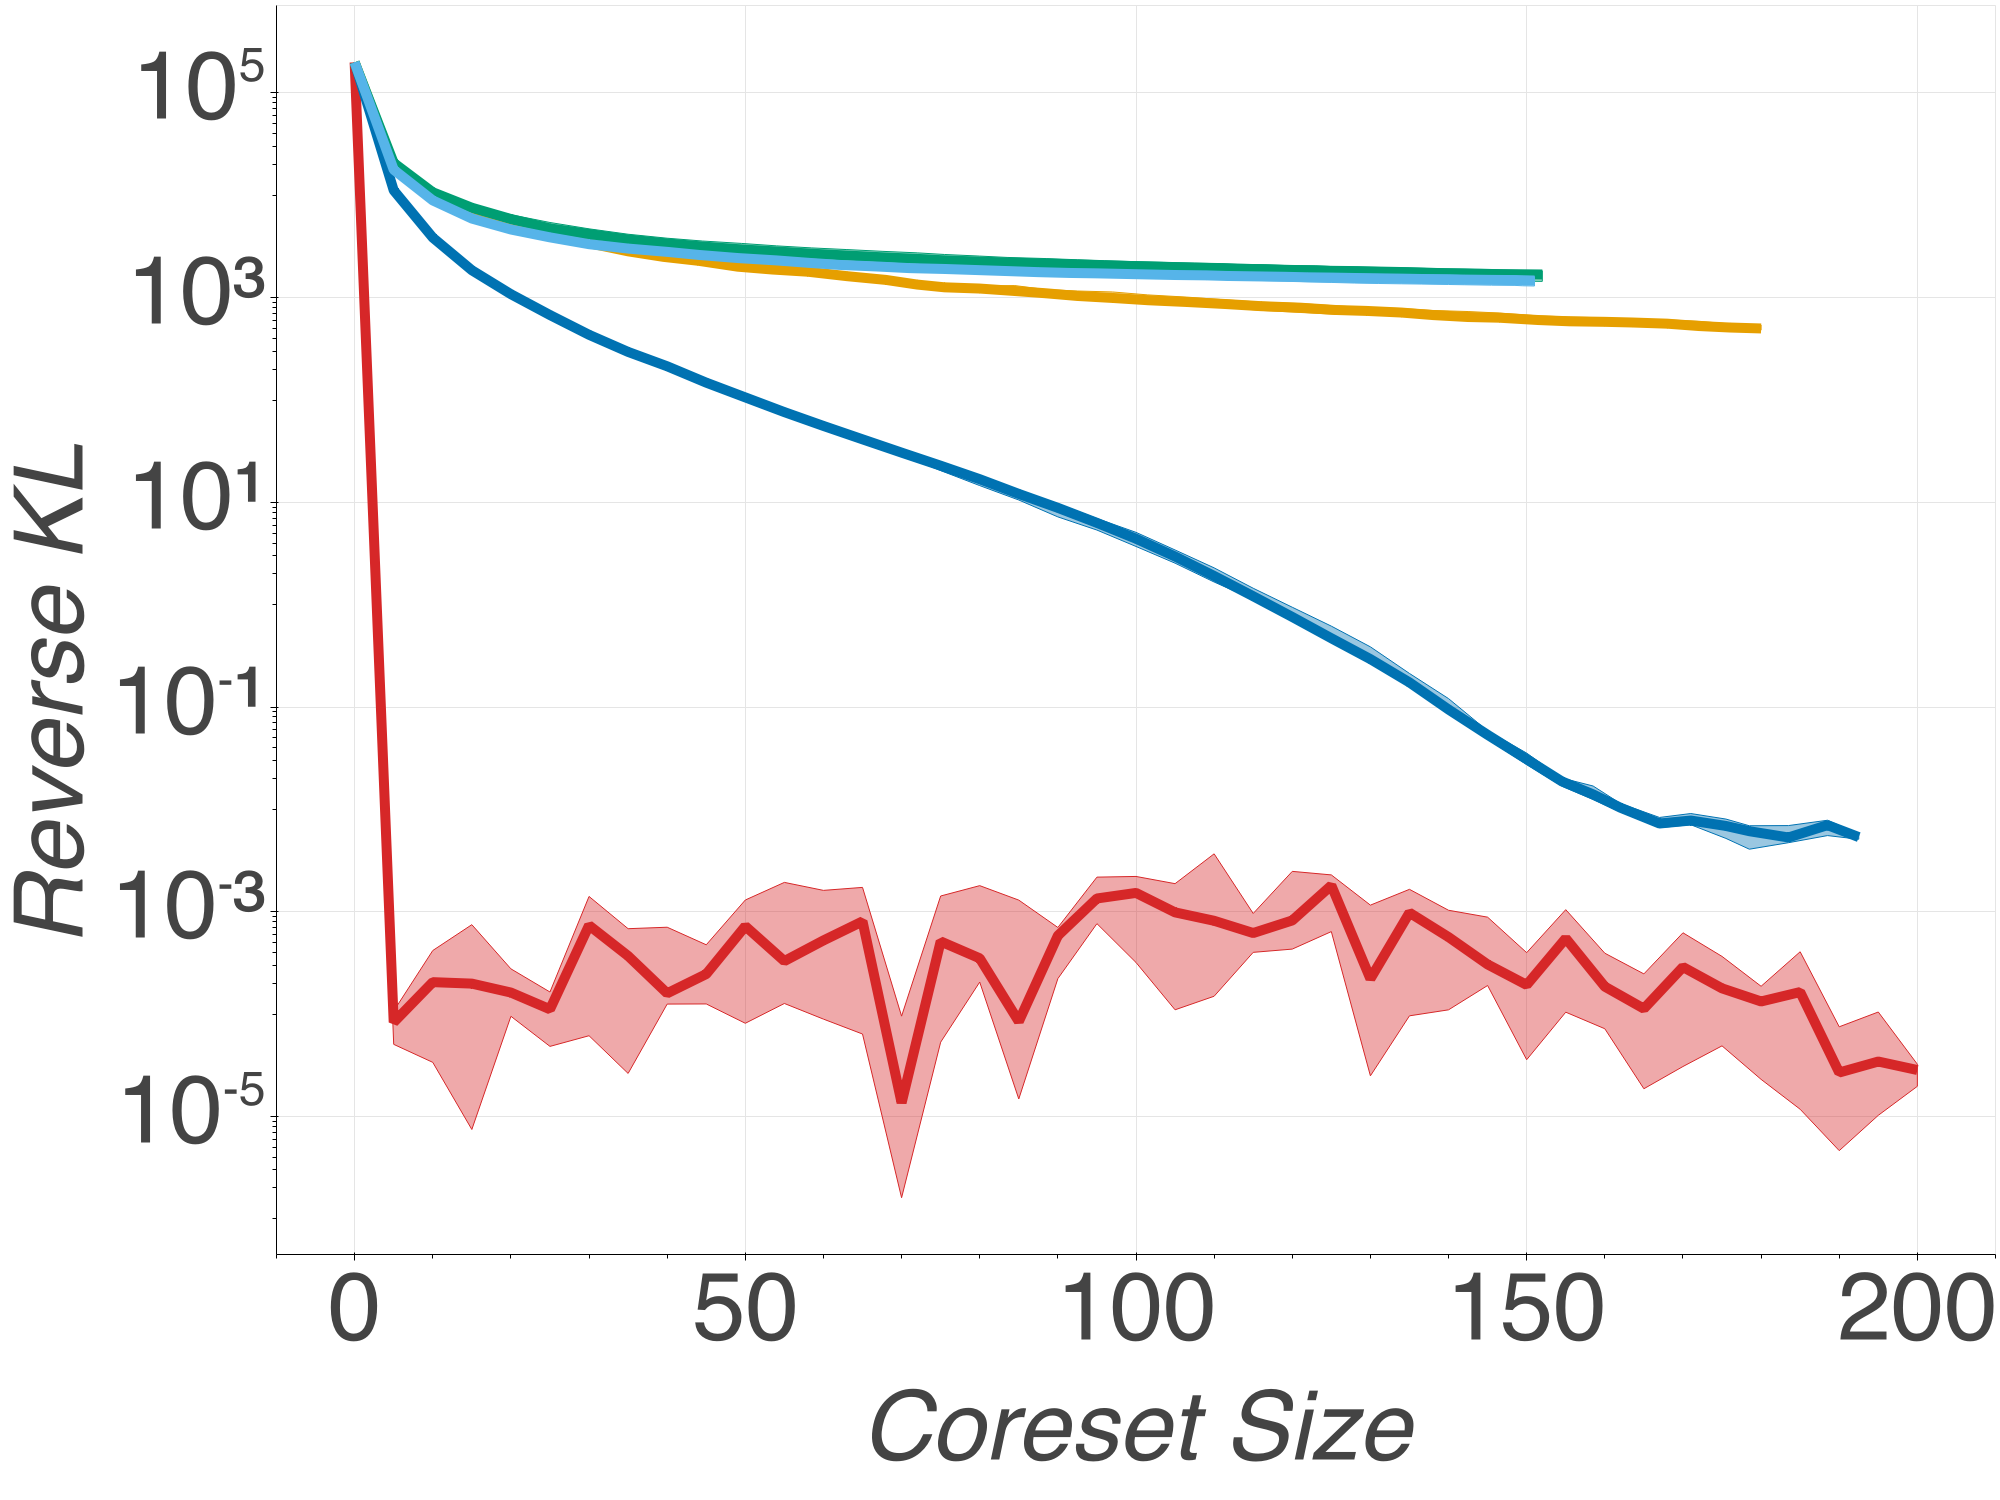
\includegraphics[ width=1.15\columnwidth]{\MyPath/figs/d200_KLDvsCstSize.png}}}%
                       \caption{(a) Gaussian mean inference, $d=200$\label{fig:gauss_mean_200}}
	\end{subfigure}\hfill\qquad
	\begin{subfigure}[c]{.29\textwidth}
			\centerline{\scalebox{1}{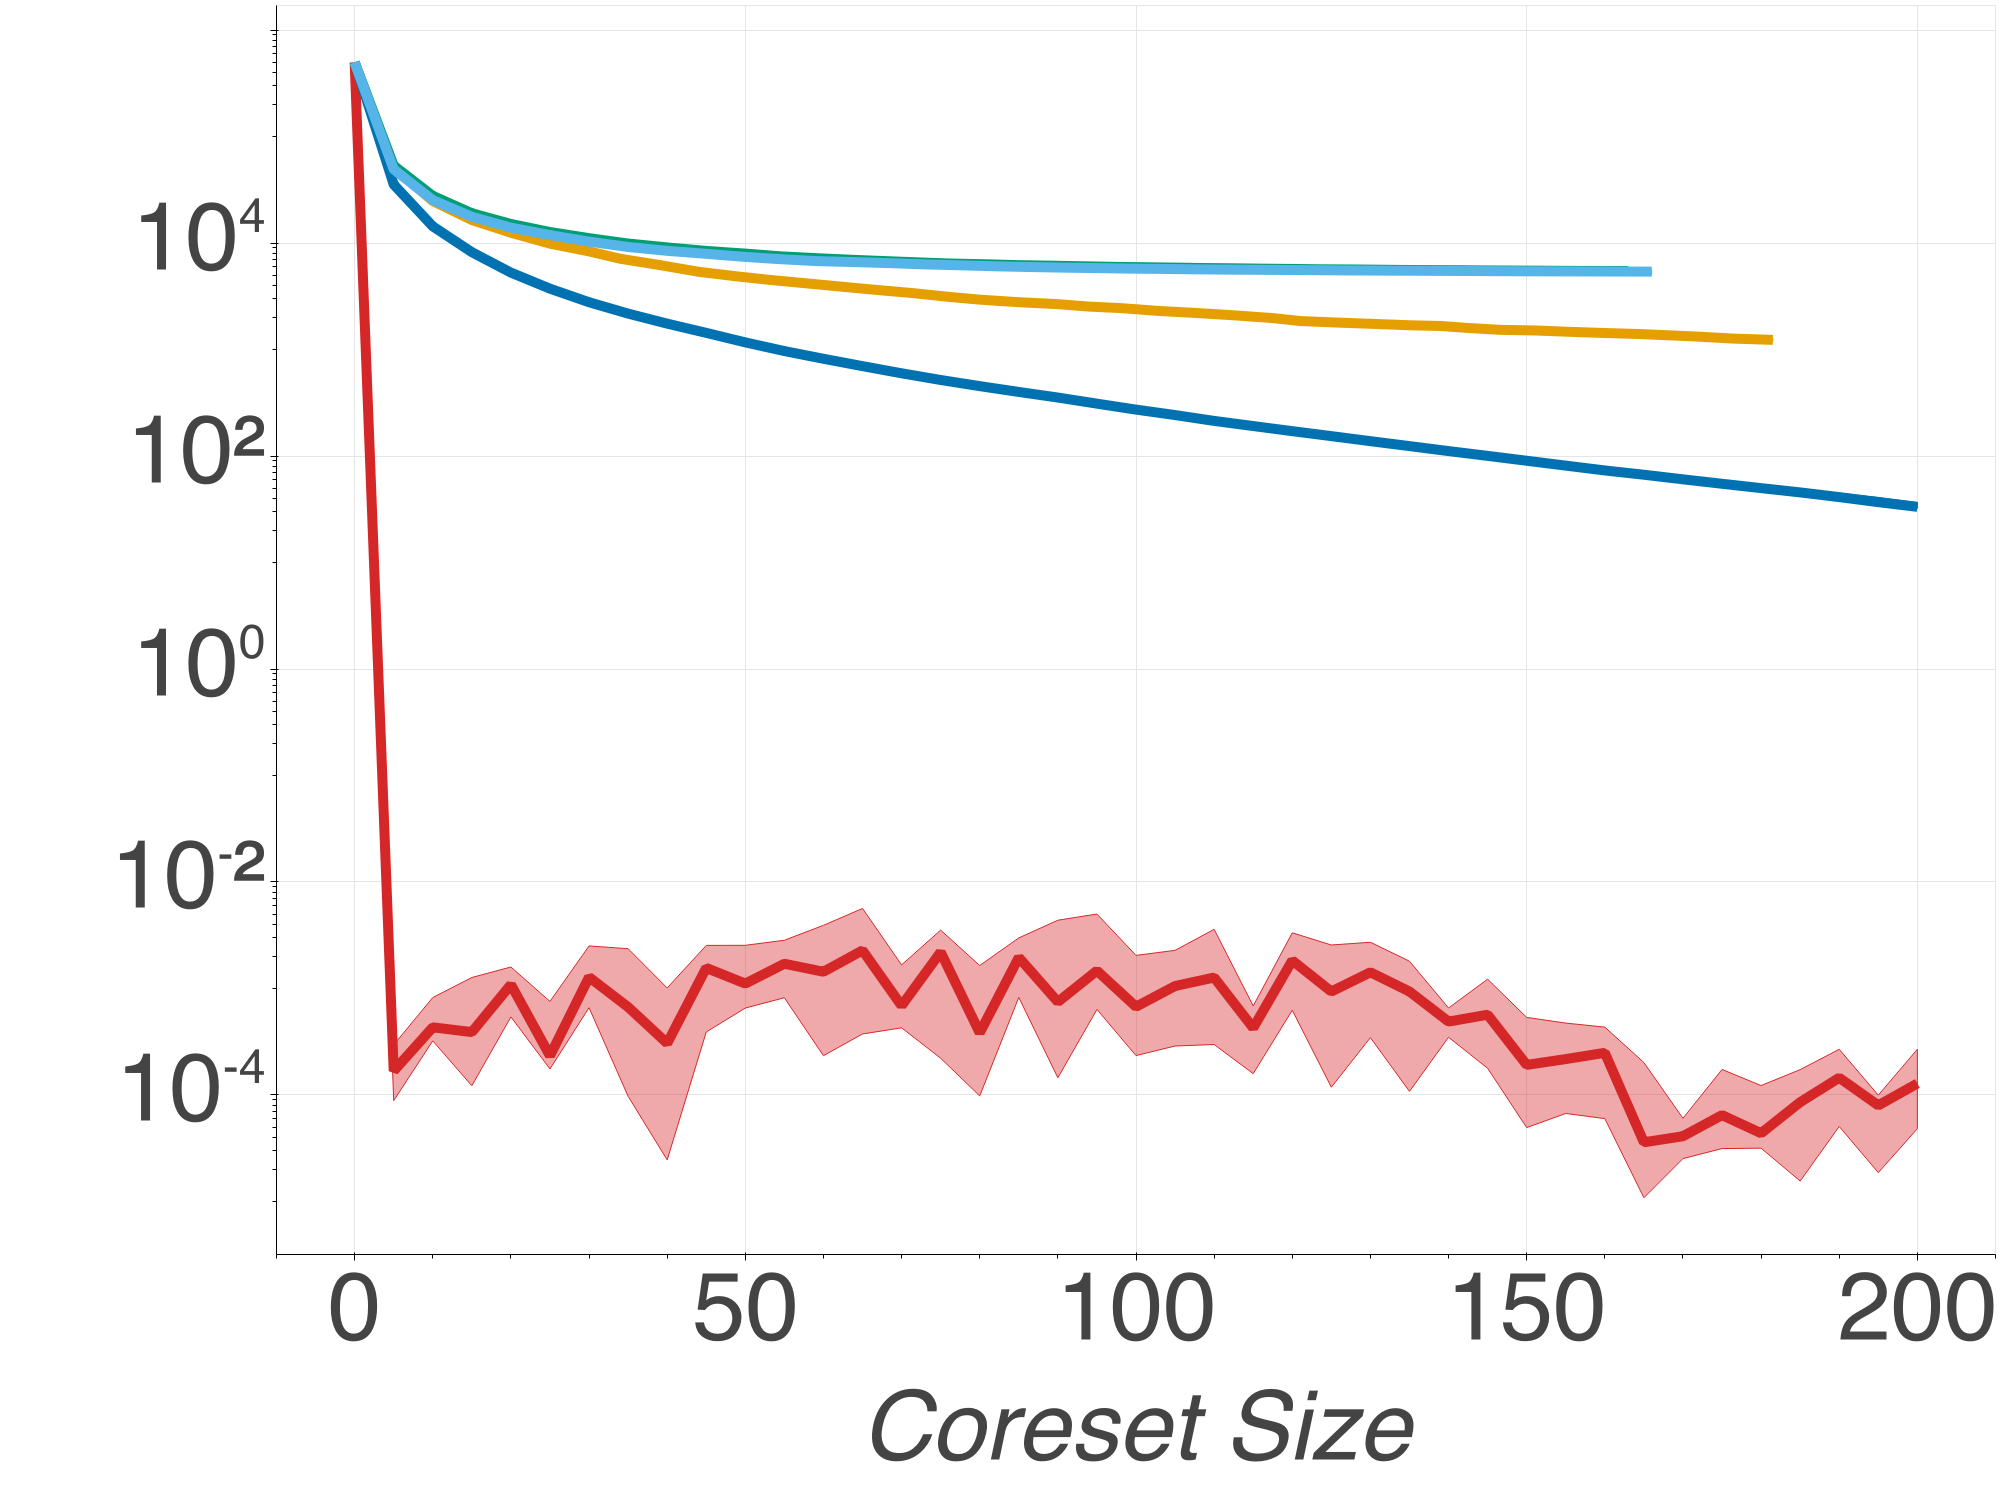
\includegraphics[ width=1.15\columnwidth]{\MyPath/figs/d500_KLDvsCstSize.png}}}%
				\caption{(b) Gaussian mean inference, $d=500$\label{fig:gauss_mean_500}}
	\end{subfigure}\hfill\qquad
	\begin{subfigure}[c]{.29\textwidth}
			\centerline{\scalebox{1}{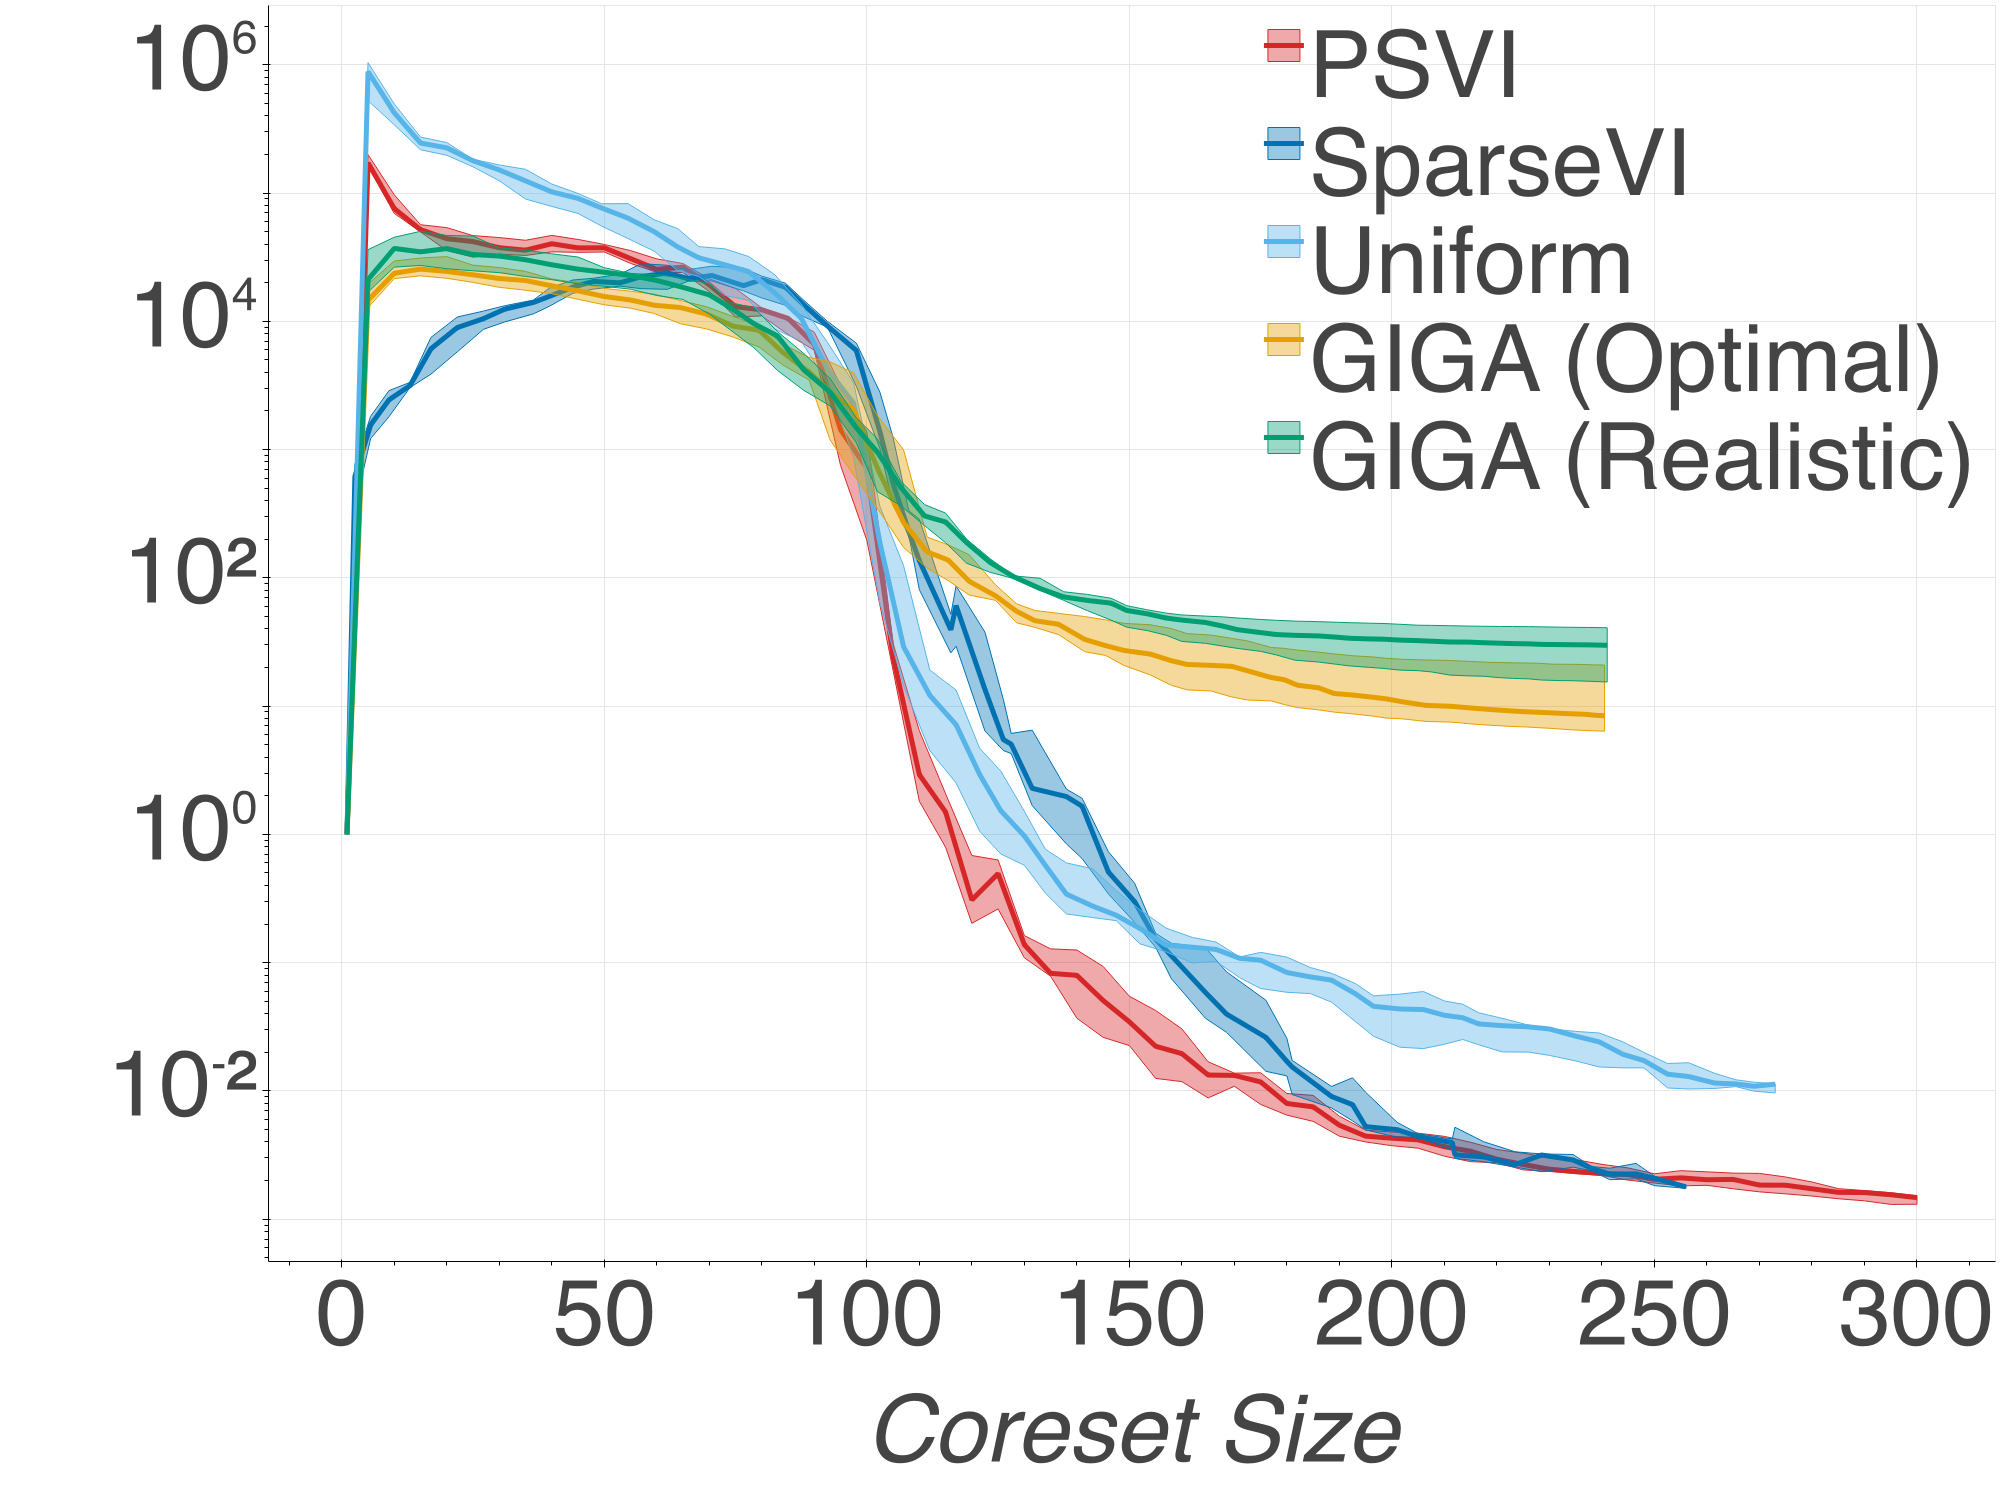
\includegraphics[width=1.15\columnwidth]{\MyPath/figs/linregKLDvsCstSize.png}}}%
				\caption{(c) Bayesian linear regression, $d=100$\label{fig:linreg_300}}
  \end{subfigure}
	\caption{Comparison of (pseudo)coreset approximate posterior quality for experiments on synthetic datasets over {10 trials}. Solid lines display the median KL divergence, with shaded areas showing~$25^{\text{th}}$ and~$75^{\text{th}}$ percentiles of KL divergence. In \cref{fig:linreg_300}, KL divergence is normalized by the prior.}
	\label{fig:gaussian_dkl}
\end{figure*}
%
We vary the pseudocoreset size from $M=1$ to $200$, and set the total number of
iterations to $ T =  500$. We use learning rates $ \gamma_t(M) = \alpha(M)
t^{-1}$, where  $ \alpha(M) = 1 $ for \sparsevi~and $ \alpha(M) = \max(1.1 - 0.005M, 0.2)
$ for \psvi.  As verified in~\cref{fig:gauss_mean_200,fig:gauss_mean_500},
Hilbert coresets provide poor quality summarizations in the high-dimensional
regime, even for large coreset sizes.  Despite showing faster decrease of
approximation error for a larger range of coreset sizes, \sparsevi~is also
fundamentally limited by the use of the original datapoints, per
\cref{prop:original_coreset_fails}.  Furthermore, we observe that the quality of all
previous coreset methods when $d=500$ is significantly lower
compared to $d=200$. On the other hand, the KL divergence for  \psvi~decreases
significantly more quickly, giving a near perfect approximation for the true
posterior with a single pseudodata point regardless of data dimension. As
shown earlier in~\cref{fig:gaussian_coreset_points}, \psvi~has the capacity to move the
pseudodata points in order to capture the
true posterior very efficiently. 

\subsection{Bayesian linear regression}
\label{section:linreg_experiment}
In the second experiment, we use a set of ${N=2,000}$ 
$101$-dimensional datapoints $(x_n,y_n)_{n=1}^{N}$ generated as follows: $(x_n)_{n=1}^N  \distiid \distNorm(0, I),\; (y_n)_{n=1}^N  \dist [1, x_n]^T\theta + \epsilon_n,\;  (\epsilon_n)_{n=1}^{N} \distiid \distNorm(0, \sigma^2)$, and aim to infer $\theta \in \reals^{101}$. We assume a prior $\theta \dist \distNorm(\mu_0,\sigma_0^2 I)$, where $ \mu_0, \sigma_0^2$ are the dataset empirical mean and second moment, and set the noise parameter $ \sigma$ to the variance of $(y_n)_{n=1}^{N}$. We apply stochastic optimization for \psvi~construction~(also see~\cref{app:linreg_model_appendix}). We use learning rates $\gamma_t = t^{-1}$ for \sparsevi, and $\gamma_t = 0.1t^{-1}$ for \psvi, $B=200$, $T=1000$, while selection step for \sparsevi~is carried out over the full dataset. \cref{fig:linreg_300} shows that Hilbert coresets cannot improve posterior approximation in this setting with 100 random projections (see~\cref{app:linreg_plots_appendix}), 
while \psvi~achieves the fastest decay rate over sizes $ 100 \leq M \lessapprox 250$, surpassing \sparsevi.

\subsection{Bayesian logistic regression}
\label{section:logreg_experiment}

Finally, we compare (pseudo)coreset construction methods on Bayesian logistic
regression applied to 3 large~($8.4$--$100K$ datapoints, $50$--$237$
dimensions) datasets. For brevity, equations and gradients for the logistic
regression model, additional experiments on \mbox{3 smaller-scale} datasets,
full dataset descriptions, hyperparameter selection, time performance
evaluation and results on an incremental scheme for pseudocoreset construction
are deferred to~\cref{app:logreg_experiment_appendix}. 
%
  %Learning rates were tuned separately per dataset, using schedules $ {\gamma_t=\alpha t^{-\half}}$. For 	\textsc{Transactions}, \textsc{ChemReact100}, and \textsc{Music},  $ \alpha $ was respectively set to $0.05, 0.1, 0.1 $ for \sparsevi, and $10, 50, 10 $ for \psvi. 
%
 For \psvi~and \sparsevi~we use minibatch size ${B=200}$, number of gradient
updates ${T=500}$, and learning rate schedules $ \gamma_t = \alpha t^{-1}$. For
\textsc{Transactions}, \textsc{ChemReact100} and \textsc{Music}, $\alpha$ is
respectively set to 0.1, 0.1, 1 for \sparsevi, and 1, 10, 10 for \psvi. In the
selection step of \sparsevi~we use a uniform subsample of $1,000$ datapoints.
For the differentially private pseudocoreset constructions (\dpsvi), we  use a
subsampling ratio $q=2\times10^{-3}$. At each iteration we adapt the clipping
norm value $ C $ to the median norm of $( f(u_m, \theta_s) - \frac{1}{S}
\sum_{s'=1}^{S} f(u_m, \theta_{s'}))_{s=1}^{S}$ computed
over pseudodata point values $u_m$, and use noise level $\sigma=5$. We
initialise each pseudocoreset of size $ M$ via sampling $(x_m)_{m=1}^{M} \distiid
\distNorm{(0, I)}$, and sampling $\theta$, $ (y_m)_{m=1}^{M} $ from the statistical
model.

\begin{figure*}[!t]
	\centering
	\begin{subfigure}[b]{.29\textwidth}
		\subcaption{(a)~\mbox{\textsc{Transactions}~($d=50$)}}
		\vspace*{-0.26cm}
		\centerline{\scalebox{1.}{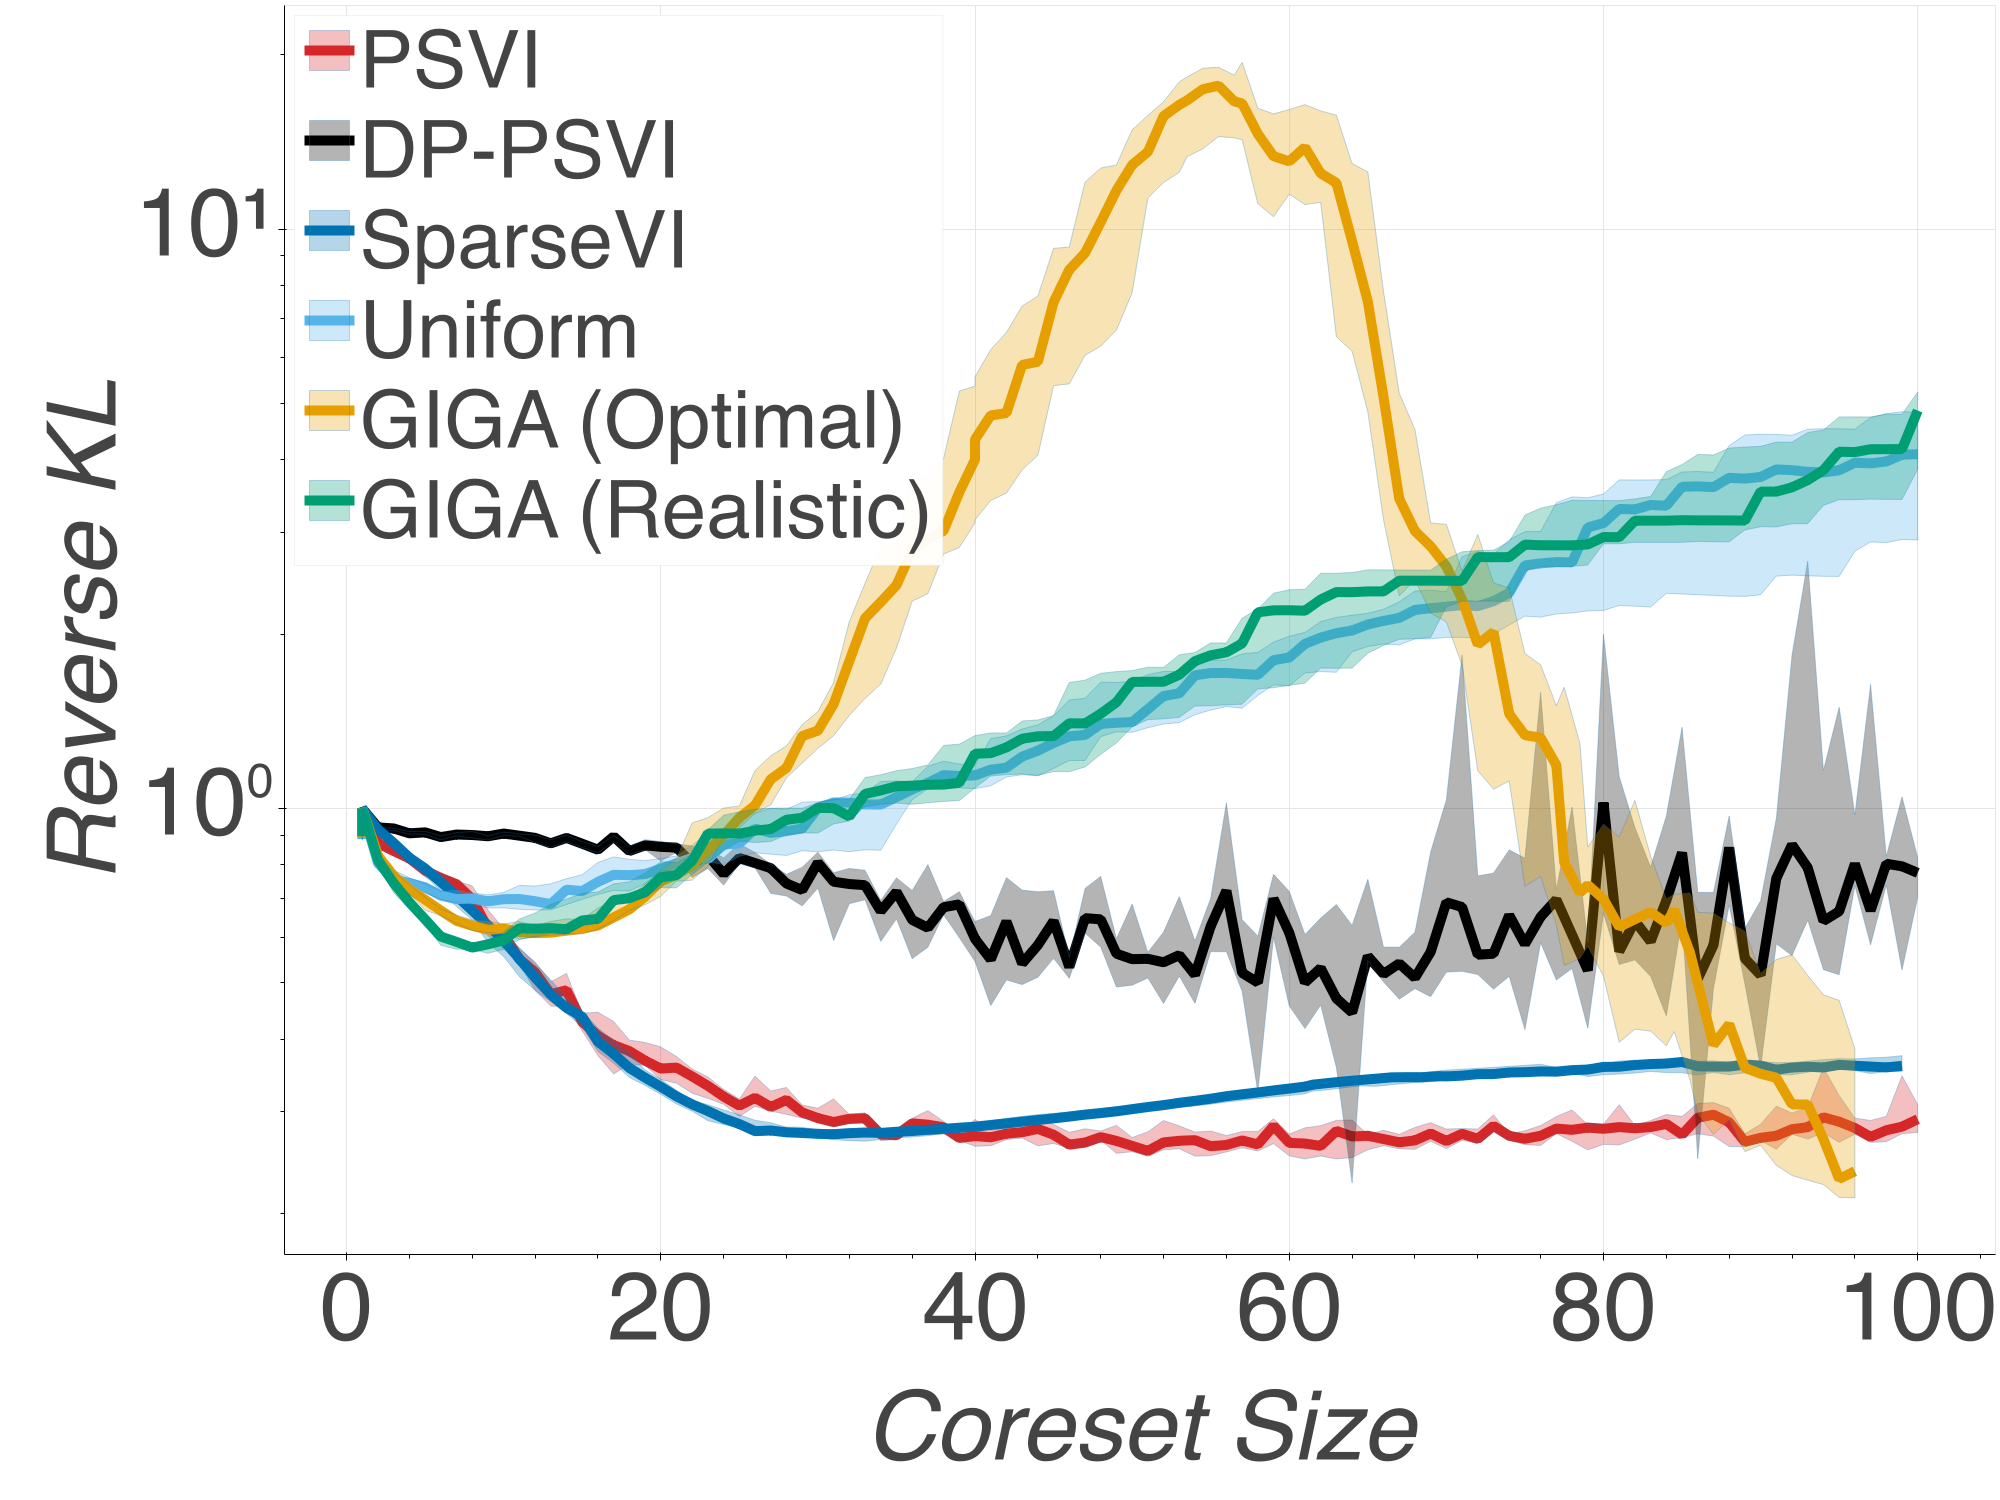
\includegraphics[width=1.15\columnwidth]{\MyPath/figs/wsanta100K_KLDvssz.png}}}%
		\label{sfig:transactions}
	\end{subfigure}\hfill\qquad
	\centering
	\begin{subfigure}[b]{.29\textwidth}
		\subcaption{(b)~\mbox{\textsc{ChemReact100}~($d=100$)}}
		\vspace*{-0.26cm}
		\centerline{\scalebox{1.}{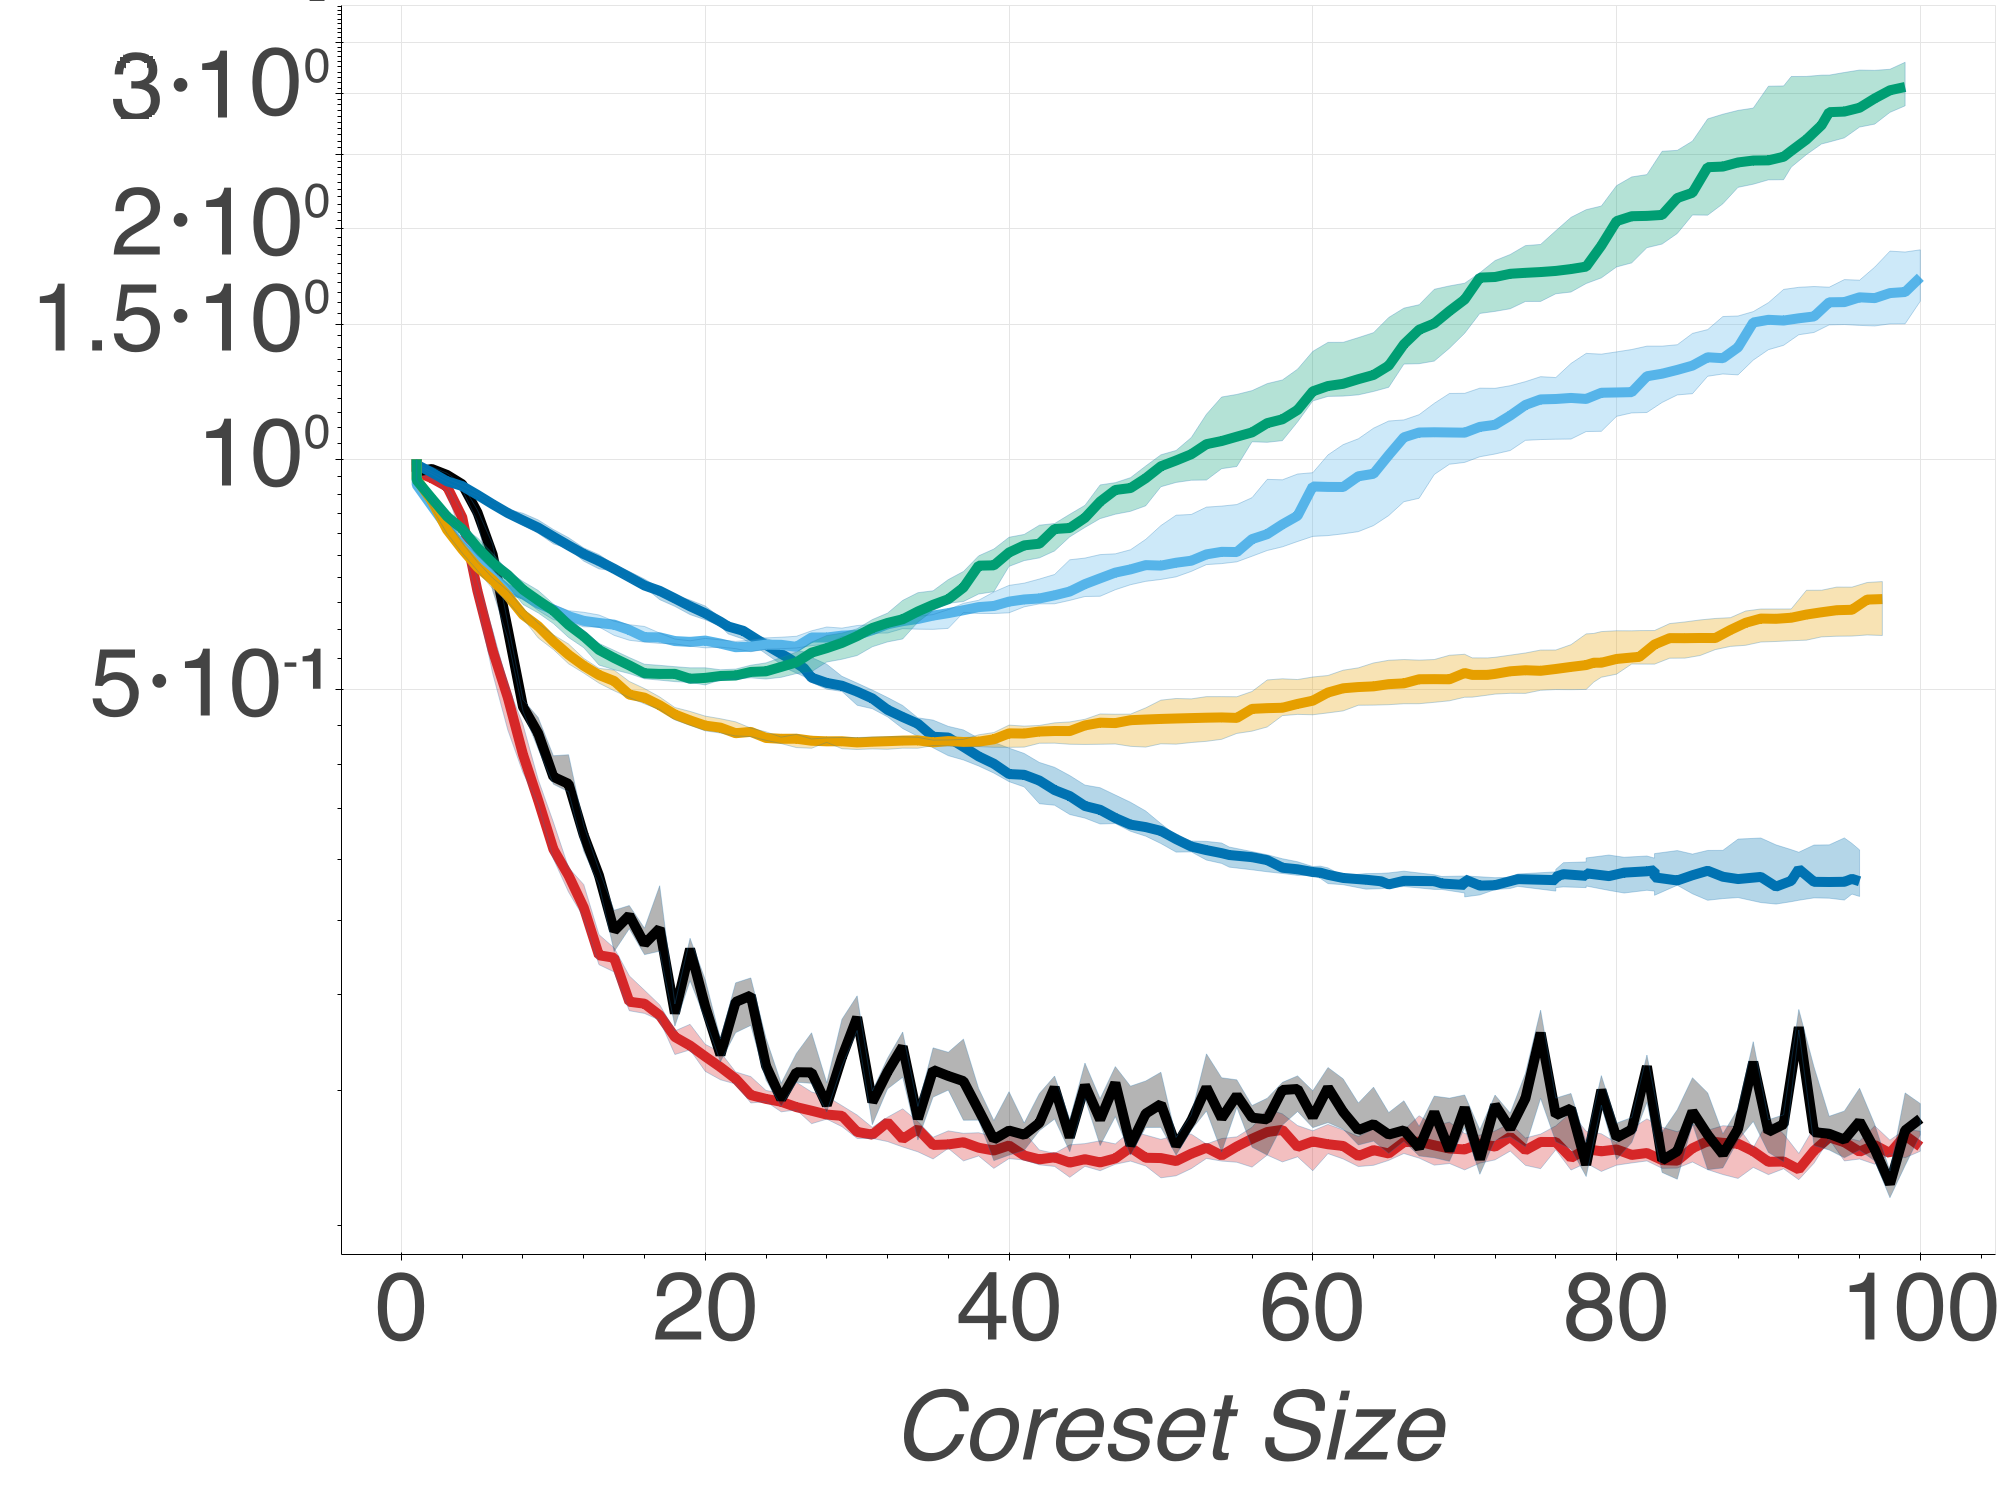
\includegraphics[width=1.15\columnwidth]{\MyPath/figs/wds1100_KLDvssz.png}}}%
		\label{sfig:chemreact100}
	\end{subfigure}\hfill\qquad
	\centering
	\begin{subfigure}[b]{.29\textwidth}
		\subcaption{(c)~\textsc{Music}~($d=237$)}
		\vspace*{-0.26cm}
		\centerline{\scalebox{1.}{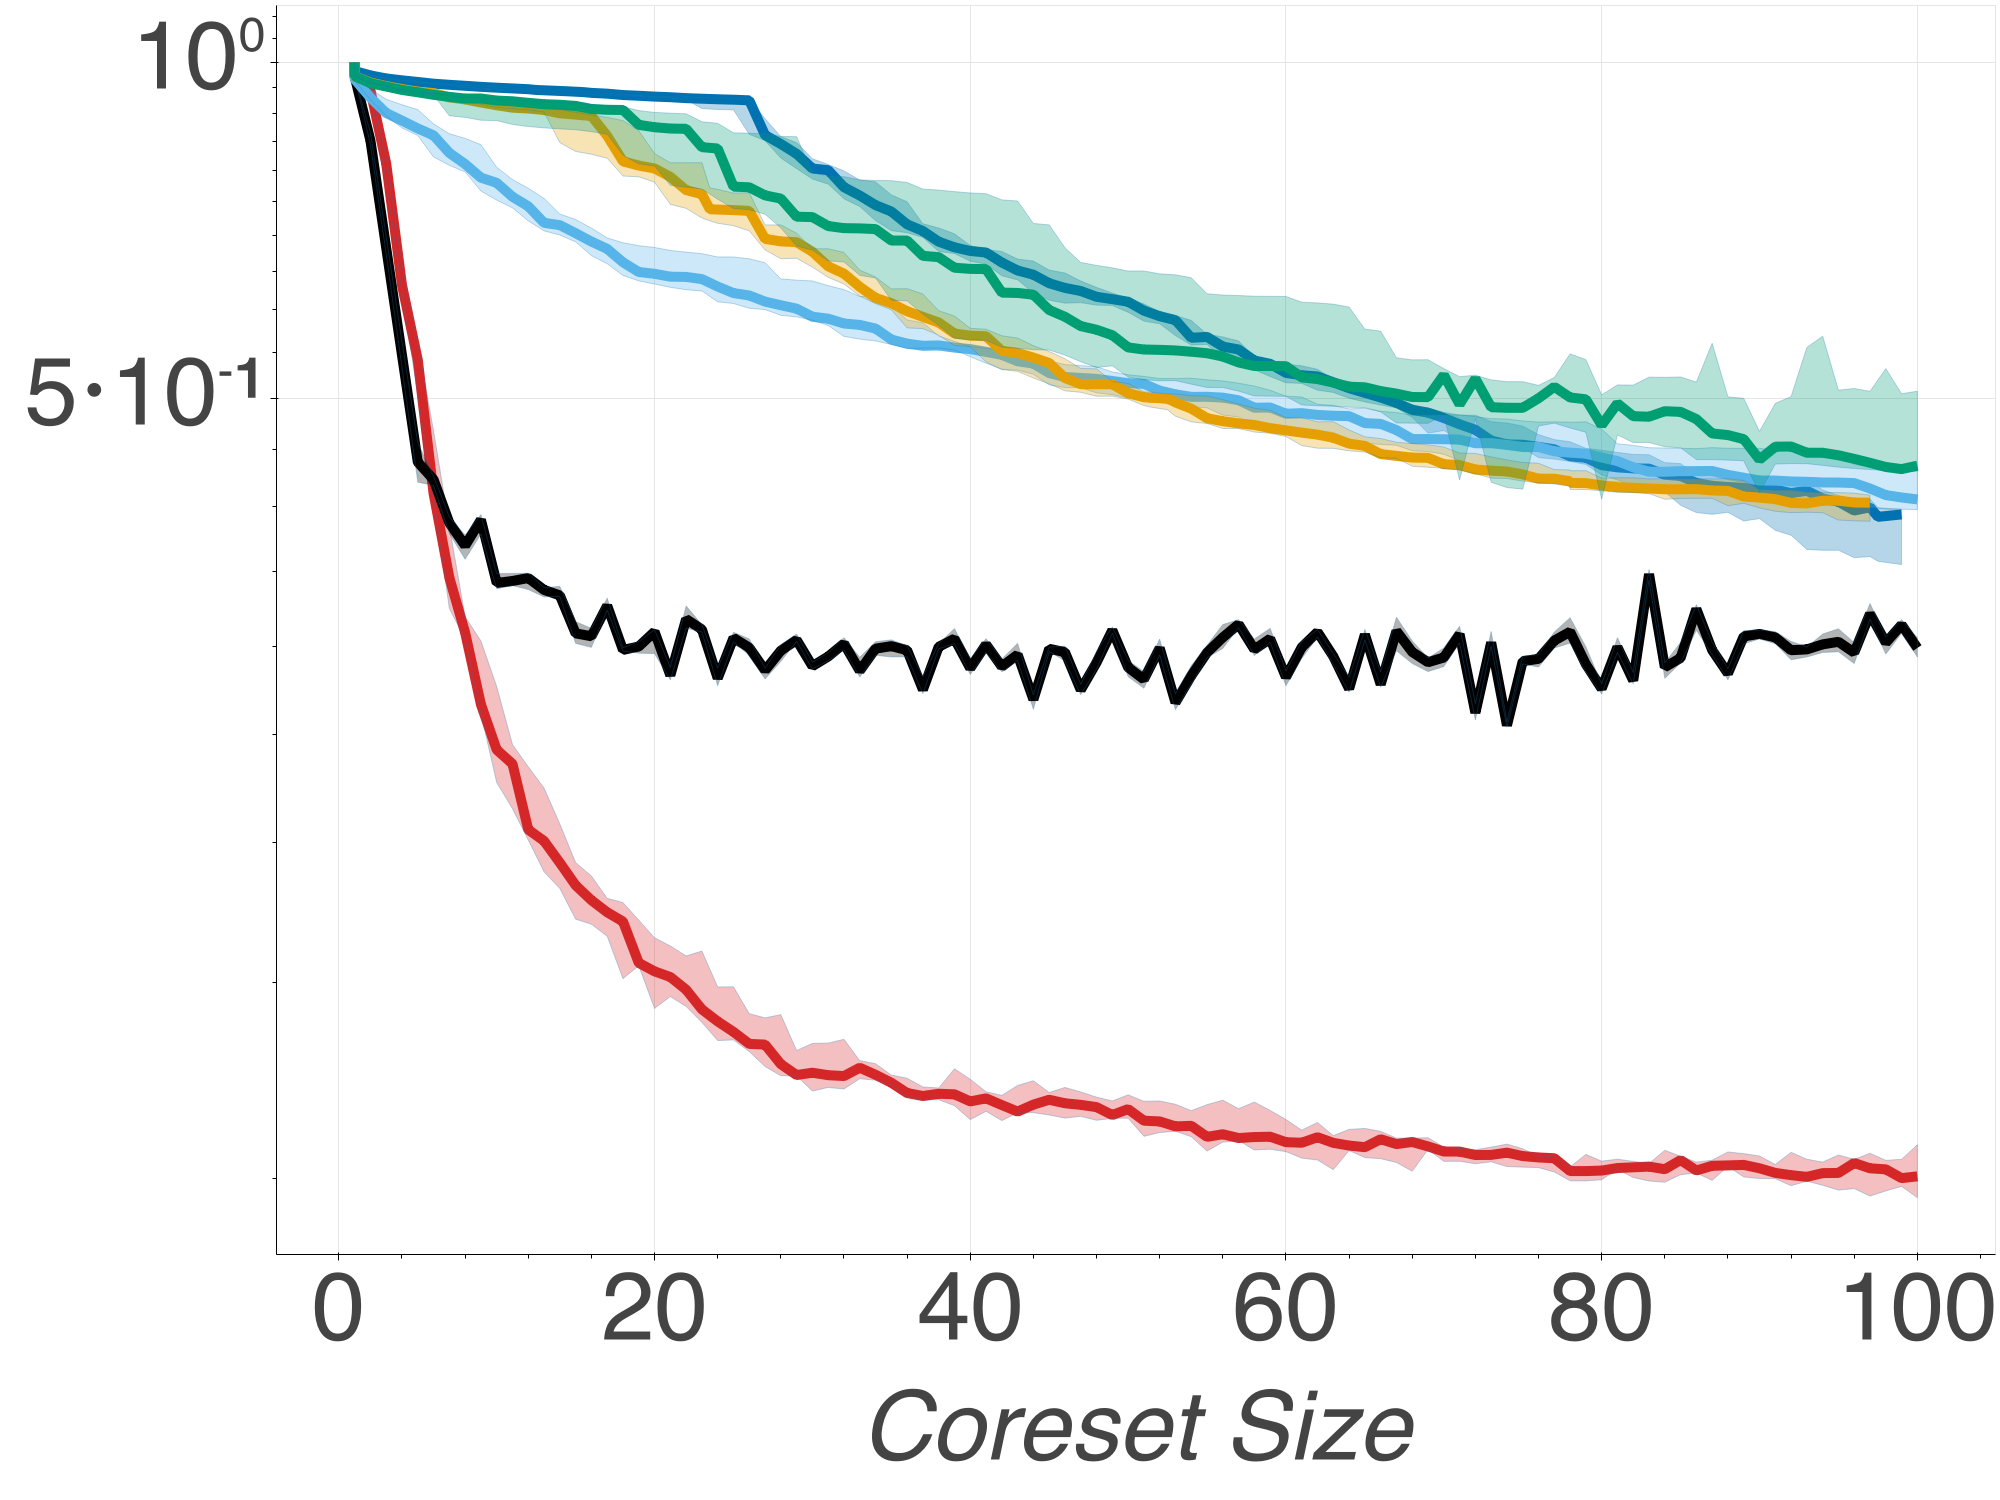
\includegraphics[width=1.15\columnwidth]{\MyPath/figs/wfma_KLDvssz.png}}}%
		\label{sfig:music}
	\end{subfigure}\hfill\qquad
	\caption{Comparison of (pseudo)coreset approximate posterior quality vs  coreset size for logistic regression over 10 trials on 3 large-scale datasets. Presented differentially private pseudocoresets  correspond to $(0.2, 1/N)$-DP. Reverse KL divergence is displayed normalized by the prior.}
	\label{fig:ls_blogreg_dkl}
\end{figure*}


\begin{figure*}[!t]
	\captionsetup[subfigure]{justification=centering}
	\centering
	\begin{subfigure}[b]{.29\textwidth}
		\subcaption{(a)~\textsc{Transactions}}
		\vspace*{-0.26cm}
		\centerline{\scalebox{1.}{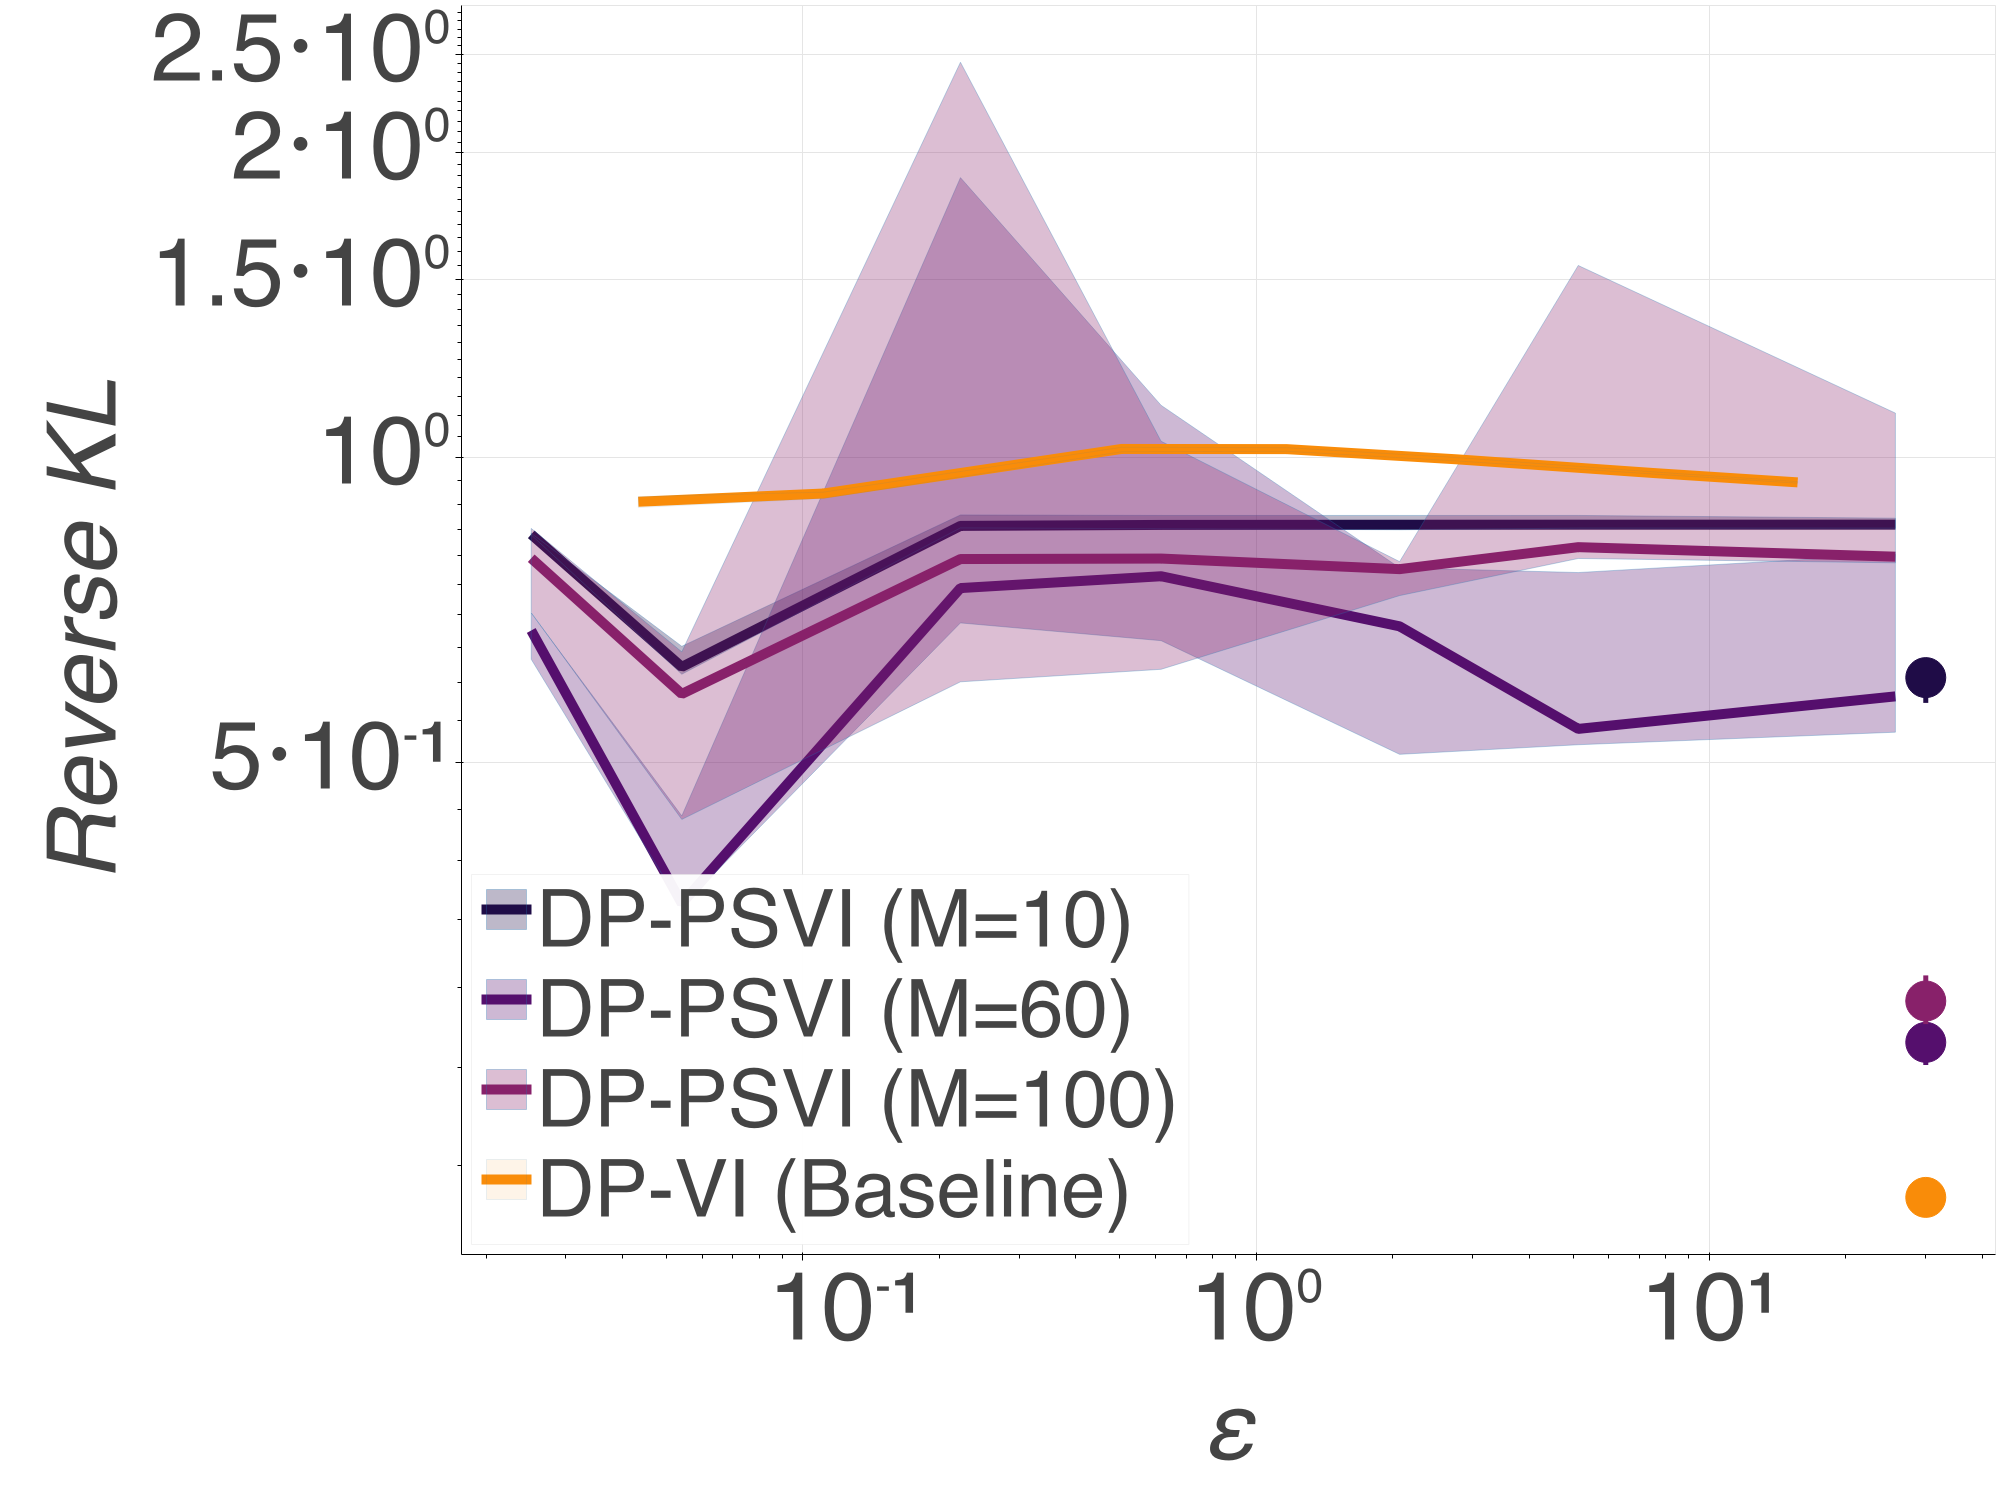
\includegraphics[width=1.15\columnwidth]{\MyPath/figs/wsanta100K_privacy.png}}}%
		\label{sfig:santapriv}
	\end{subfigure}
	\hfill\qquad
	\centering
	\begin{subfigure}[b]{.29\textwidth} 
		\subcaption{(b)~\textsc{ChemReact100}}
		\vspace*{-0.26cm}
		\centerline{\scalebox{1.}{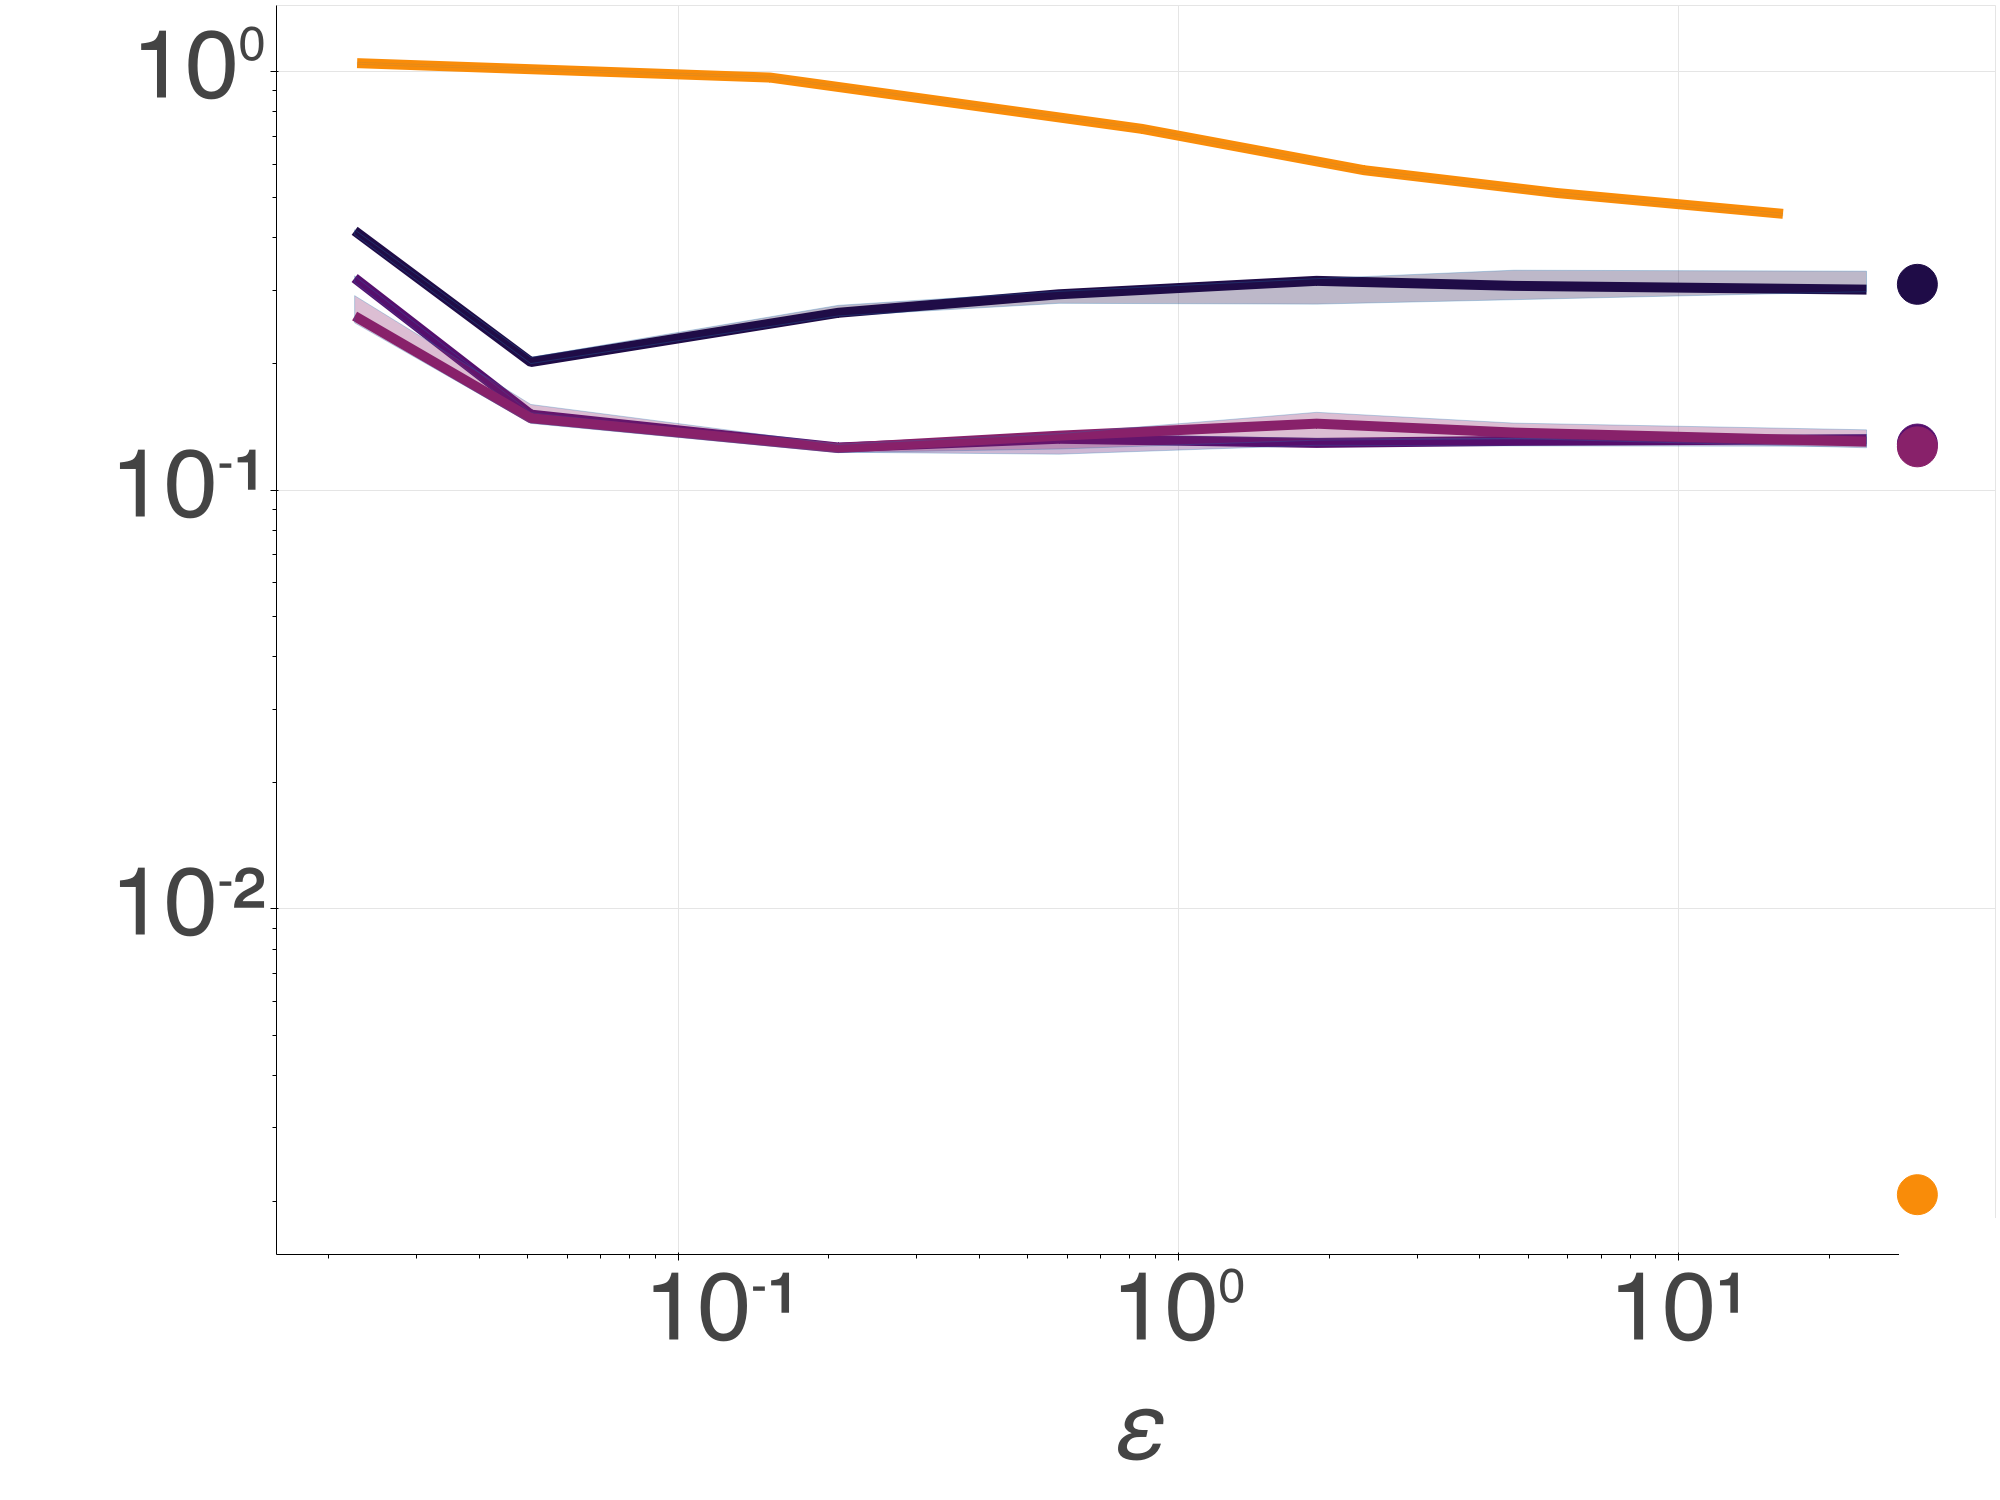
\includegraphics[width=1.15\columnwidth]{\MyPath/figs/wds1100_privacy.png}}}%
		\label{sfig:chemreact100priv}
	\end{subfigure}
	\hfill\qquad
	\centering
	\begin{subfigure}[b]{.29\textwidth}
		\subcaption{(c)~\textsc{Music}}
		\vspace*{-0.26cm}
		\centerline{\scalebox{1.}{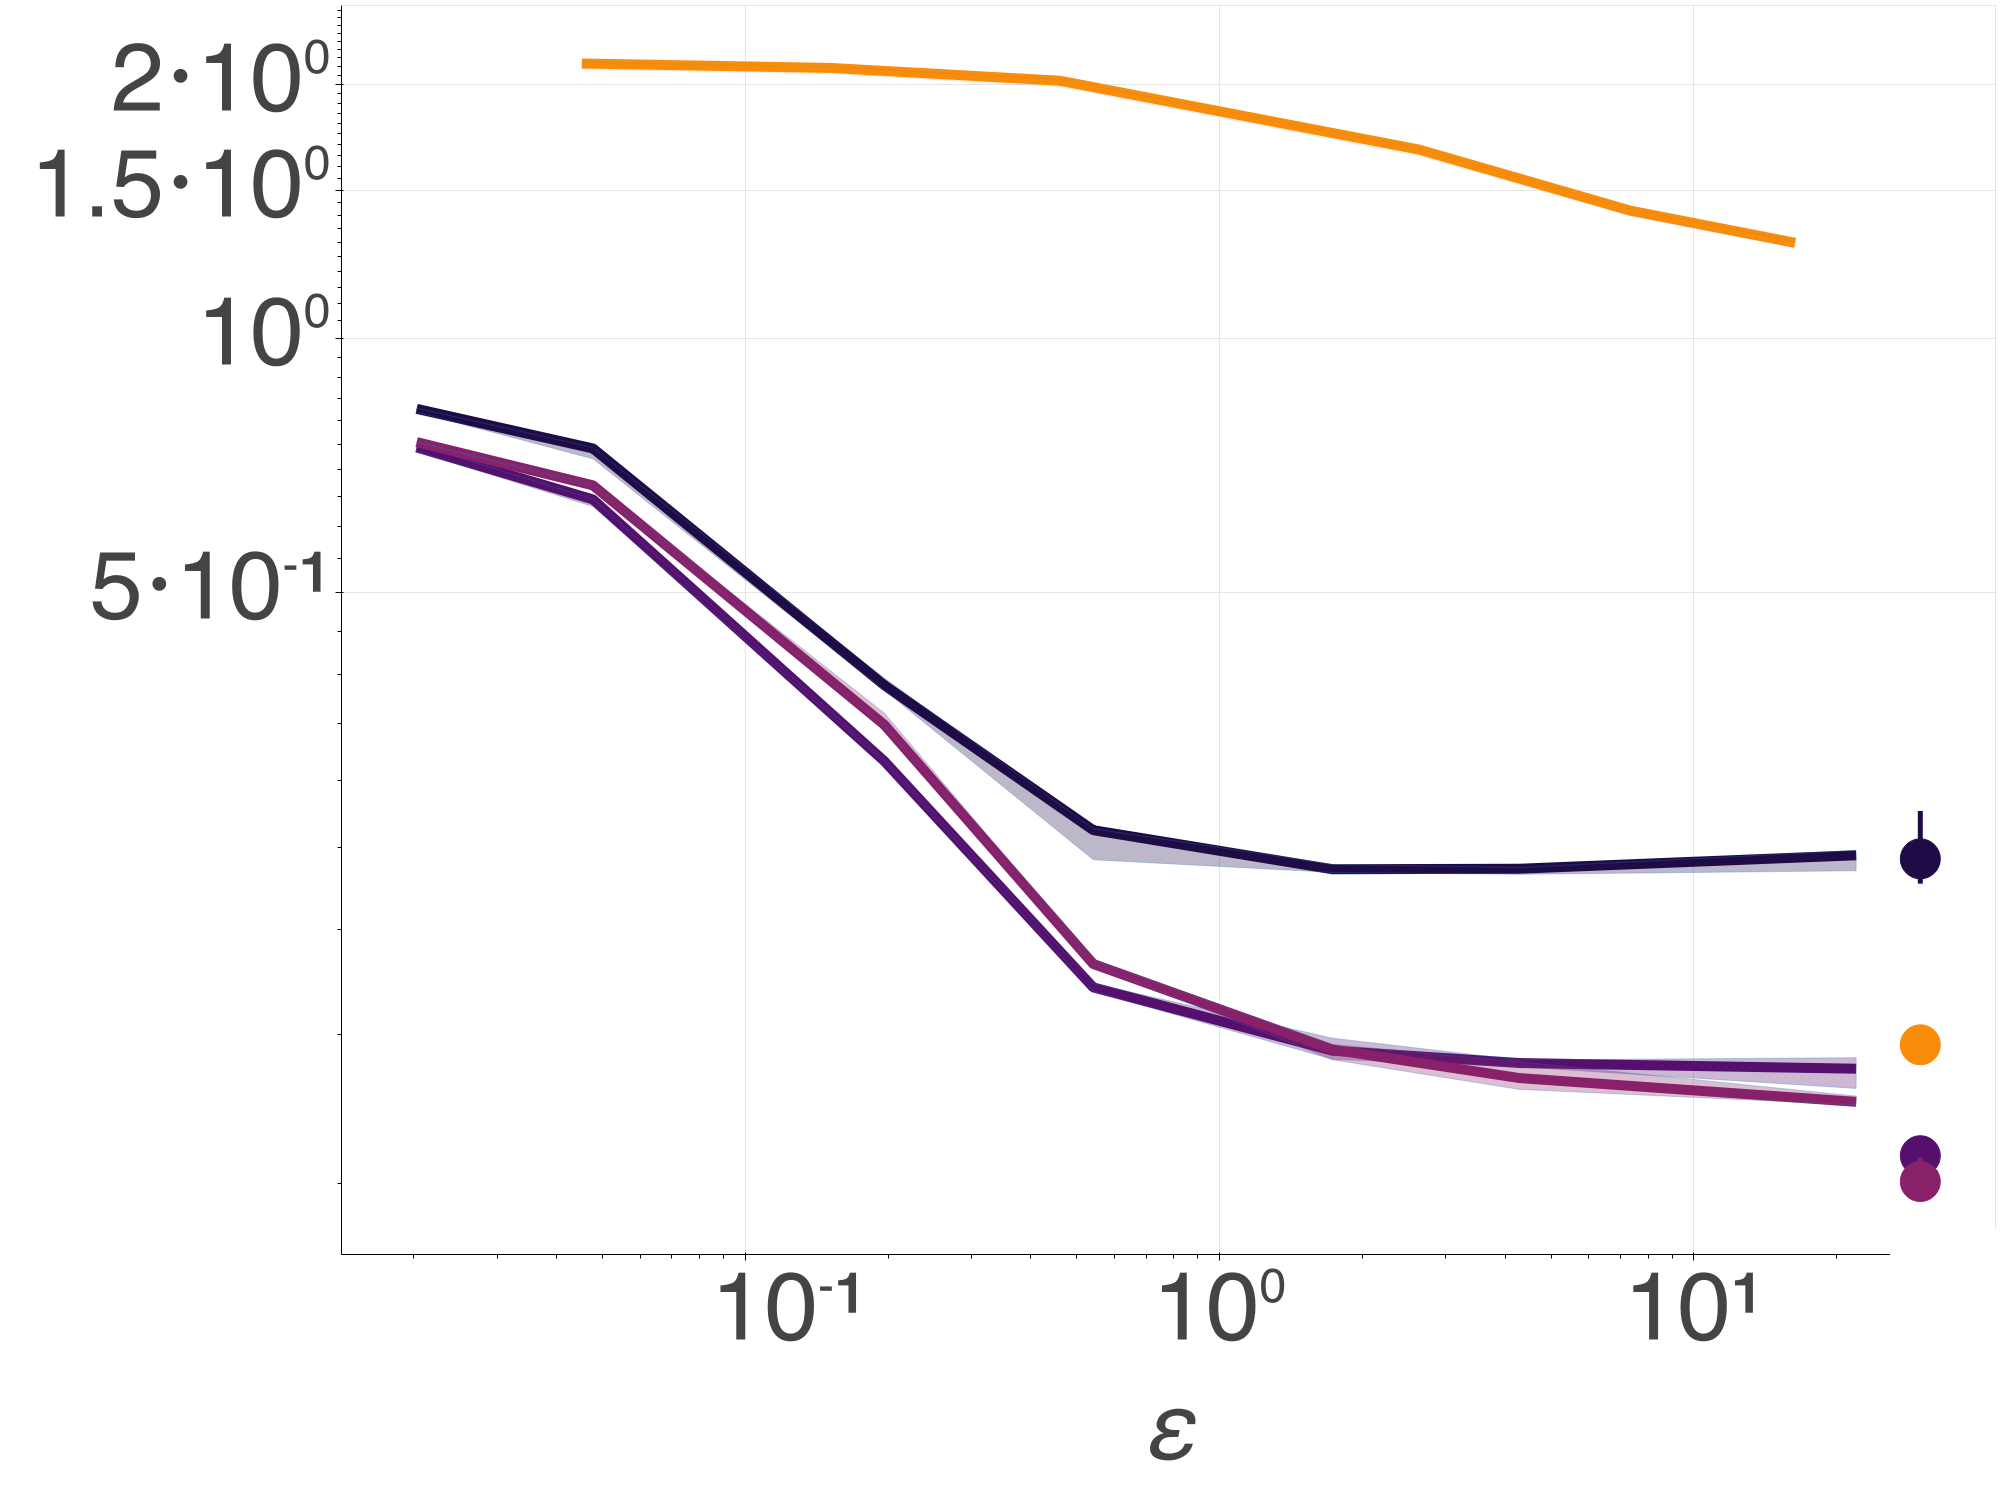
\includegraphics[width=1.15\columnwidth]{\MyPath/figs/wfma_privacy.png}}}%
		\label{sfig:musicpriv}
	\end{subfigure}
	\hfill\qquad
	\caption{Approximate posterior quality over decreasing differential privacy guarantees for private pseudocoresets of varying size~(\dpsvi) plotted against private variational inference~(\dpvi, \citep{jalko17}). $\delta$ is always kept fixed at $ 1/N$. Markers on the right end of each plot display the errorbar of approximation achieved by the corresponding nonprivate posteriors. Results are displayed over 5 trials for each construction.}
	\label{fig:dklvseps} 
\end{figure*}


Results presented in~\cref{fig:ls_blogreg_dkl} demonstrate that \psvi~achieves consistently the smallest posterior approximation error in the small coreset size regime, offering improvement
compared to \sparsevi~and being competitive with \gigao,
without the requirement for specifying a weighting function. In~\cref{sfig:transactions}, for $M \geq d$ ~\gigao~follows a much steeper decrease in KL divergence, reflecting the dependence of its approximation quality on dataset dimension per~\cref{prop:original_coreset_fails}. In contrast, \psvi~typically reaches its minimum at $M<d$. The difference in approximation quality becomes clearer in higher dimensions~(e.g. \textsc{Music}, where $d=237$). Perhaps surprisingly, the private pseudocoreset construction has only marginally worse approximation quality compared to nonprivate \psvi~and generally achieves better peformance in comparison to the other state-of-the-art nonprivate coreset constructions. 
In~\cref{fig:dklvseps} we present the achieved posterior approximation quality via \dpsvi, against a competitive state-of-the-art method for general-purpose private inference(\dpvi, \cite{jalko17}). For logistic regression, \dpvi~infers an approximate posterior from the family of Gaussians with diagonal covariance via ADVI~\citep{kucukelbir17}, followed by an additional Laplace approximation. Note that by design, \dpvi~is constrained by the usual Gaussian variational approximation, while \dpsvi~is more flexible and can approach the true posterior as $ M $ increases---this effect is reflected in nonprivate posteriors as well as data dimensionality grows~(see for example~\cref{sfig:musicpriv}). Indeed, we verify that in the high-privacy regime \dpsvi~for sufficient pseudocoreset size (which is typically small for tested real-world datasets) offers posterior approximation with better KL divergence compared to \dpvi. Our findings indicate that private \psvi~offers efficient releases of big data via informative pseudopoints, which enable arbitrary post processing (e.g. running any \emph{nonprivate} black-box algorithm for Bayesian inference), under strong privacy guarantees and without reducing the quality of inference.








\section{Conclusions}
We introduced a new variational formulation for Bayesian coreset construction, which yields efficient summarizations for big and high-dimensional datasets via simultaneously learning pseudodata points locations and weights. We proved limitations of existing variational formulations for coresets and demonstrated that they can be resolved with our new methodology. We proposed an efficient construction scheme via black-box stochastic optimization and showed how it can be adapted for differentially private Bayesian summarization. Finally, we demonstrated the applicability of our methodology on synthetic and real-world datasets, and practical statistical models.  

%\textcolor{red}{Presented work can be further pursued in several directions: Although our experiments demonstrated similar levels of variance with \sparsevi, we think that existing variance reduction techniques~\citep{ranganath14} might allow improvement in our stochastic optimization. Furthermore, privacy accounting can become tighter via adapting it to the specific form of private computations entering gradients in \dpsvi. Learned pseudodata points are expected to offer an even larger improvement in statistical models where there is a stronger interdependence between datapoints and parameters---e.g. point processes---compared to i.i.d. settings. Last but not least, an information-geometric interpretation of our approximation can shed more light on the theoretical understanding of \psvi. We leave the above as topics for future research.} 

Pseudocoreset variational inference is a general-purpose Bayesian inference
algorithm, hence shares implications mostly encountered in approximate
inference methods. For example, replacing the full dataset with a
pseudocoreset has the potential to cause inferential errors; these can be
partially tempered by using a pseudocoreset of larger size. Note also
that the optimization algorithm in this work aims to reduce 
KL divergence: however the proposed
variational objective might be misleading in many applications and lead to
incorrect conclusions in certain statistical models (e.g. point estimates and
uncertainties might be far off despite KL being almost zero~\citep{huggins20}).
Moreover, Bayesian inference in general is prone to model misspecification.
Therefore, a pseudocoreset summarization based on a wrong statistical model
will lead to non-representative compression for inferential purposes.
Constructing the coreset on a statistical model suited for robust inference
instead of the original one~\citep{miller19, wang17}, can offer protection
against modeling mismatches. Naturally, the utility of generated dataset
summary becomes task-dependent, as it has been optimized for a specific
learning objective, and cannot be fully transferable to multiple different
inference tasks on the same dataset.

Our learnable pseudodata are also generally not as interpretable 
as the points of previous coreset methods, as they are not real data. And the level of 
interpretability is model specific. This creates a risk of misinterpretation
of pseudocoreset points in practice. On the other hand, our optimization framework
does allow the introduction of interpretability constraints (e.g.~pseudodata sparsity)
to explicitly capture interpretability requirements.

Pseudocoreset-based summarization is susceptible to reproducing potential
biases and unfairness existing in the original dataset. Majority-group datapoints in the full dataset which capture information relevant to the
statistical task of interest are expected to remain over-represented in the
learned summary; while minority-group datapoints might be eliminated, if their
distinguishing features are not related to inference. Amending the
initialization step to contain such datapoints or using a prior that
strongly favors a debiased version of the dataset could both mitigate these
concerns; but more study is warranted.


%\section*{ Broader Impact}
\label{sec:broader_impact}

Pseudocoreset variational inference is a general-purpose Bayesian inference
algorithm, hence shares implications mostly encountered in approximate
inference methods. For example, replacing the full dataset with a
pseudocoreset has the potential to cause inferential errors; these can be
partially tempered by using a pseudocoreset of larger size. Note also
that the optimization algorithm in this work aims to reduce 
KL divergence: however the proposed
variational objective might be misleading in many applications and lead to
incorrect conclusions in certain statistical models (e.g. point estimates and
uncertainties might be far off despite KL being almost zero~\citep{huggins20}).
 Moreover, Bayesian inference in general is prone to model misspecification.
Therefore, a pseudocoreset summarization based on a wrong statistical model
will lead to non-representative compression for inferential purposes.
Constructing the coreset on a statistical model suited for robust inference
instead of the original one~\citep{miller19, wang17}, can offer protection
against modelling mismatches. Naturally, the utility of generated dataset
summary becomes task-dependent, as it has been optimized for a specific
learning objective, and cannot be fully transferable to multiple different
inference tasks on the same dataset.

Our learnable pseudodata are also generally not as interpretable 
as the points of previous coreset methods, as they are not real data. And the level of 
interpretability is model specific. This creates a risk of misinterpretation
of pseudocoreset points in practice. On the other hand, our optimization framework
does allow the introduction of interpretability constraints (e.g.~pseudodata sparsity)
to explicitly capture interpretability requirements.

Pseudocoreset-based summarization is susceptible to reproducing potential
biases and unfairness existing in the original dataset. Majority-group datapoints in the full dataset which capture information relevant to the
statistical task of interest are expected to remain over-represented in the
learned summary; while minority-group datapoints might be eliminated, if their
distinguishing features are not related to inference. Amending the
initialization step to contain such datapoints or using a prior that
strongly favors a debiased version of the dataset could both mitigate these
concerns; but more study is warranted.

%\section{Technical Results and Proofs}
\label{supp:proofs}

\subsection{Proof of~\cref{prop:original_coreset_fails}}
In the setting of~\cref{prop:original_coreset_fails}, both the exact posterior and the coreset posterior 
are multivariate Gaussian distributions, denoted as $\distNorm{\left(\mu_1, \Sigma_1\right)}$ and 
$\distNorm{\left(\mu_{w}, \Sigma_{w}\right)}$ respectively. 
The mean and covariance are
\[
\Sigma_{1}=\frac{1}{1+ N} I_d, \quad \mu_{1}=\Sigma_{1}\left( \sum_{n=1}^{N} X_{n}\right), 
\label{eq:exact_post}
\]
and
\[
\label{eq:coreset_post}
\hspace{-.3cm}\Sigma_{w}\!=\!\frac{I_d}{1+ \left(\sum_{n=1}^N w_n\right)}, 
\quad
\mu_{w}\!=\!\Sigma_{w}\left( \sum_{n=1}^{N} w_n X_{n}\right).
\]

\begin{proof}[Proof of~\cref{prop:original_coreset_fails}]
By~\cref{eq:exact_post,eq:coreset_post}, 
\begin{equation} \label{eq:KL_from_coreset_post_to_exact}
\begin{aligned}
\kl{\pi_{w}}{\pi_1}
 =& \frac{1}{2}\left[\log\frac{|\Sigma_{1}|}{|\Sigma_{w}|} - d + \tr\left( \Sigma_{1}^{-1}\Sigma_{w}\right)   
  (\mu_{1} - \mu_{w})^T \Sigma_{1}^{-1}(\mu_{1} - \mu_{w})\right]\\
=& \frac{1}{2} \left[ -d\log \left( \frac{1+ N}{1+ \sum_{n=1}^N w_n}\right) - d  + d \left( \frac{1+ N}{1+ \sum_{n=1}^N w_n}\right)
+  (\mu_{1} - \mu_{w})^T \Sigma_{1}^{-1}(\mu_{1} - \mu_{w})\right].
\end{aligned}
\end{equation}
Note that $\forall x > 0, x-1 \geq \log x$, implying that 
$$ d\log \left( \frac{1+ N}{1+ \sum_{n=1}^N w_n}\right) -d + d \left( \frac{1+ N}{1+ \sum_{n=1}^N w_n}\right) > 0.$$ 
Thus, 
\begin{equation} \label{eq:first_inequality}
\kl{\pi_{w}}{\pi_1} \geq \frac{1}{2}(\mu_{1} - \mu_{w})^T \Sigma_{1}^{-1}(\mu_{1} - \mu_{w}).
\end{equation}

Suppose we pick a set $\mcI\subseteq[N]$, $\left|\mcI\right| = M$ of active indices $n$ where the optimal $w_n \geq 0$,
 and enforce that all others $n\notin \mcI$ satisfy $w_n = 0$.
Then denoting
\[
Y = \left[X_n : n\notin \mcI\right] \in \reals^{d\times (N-M)}, \quad
X = \left[X_n : n\in \mcI\right] \in \reals^{d\times M},
\]
we have that for any $w\in \reals_+^M$ for those indices $\mcI$,
\[
\kl{\pi_w}{\pi_1} 
\geq & \frac{1}{2(N+1)}1^TY^TY1 
+1^TY^TX\left(\frac{1}{N+1} - \frac{w}{1+1^Tw}\right)\\
&+\frac{N+1}{2}\!\!\left(\frac{1}{N+1}\! -\! \frac{w}{1+1^Tw}\right)^T\!\!\!\!\!X^T\!X\!\left(\frac{1}{N+1} \!-\! \frac{w}{1+1^Tw}\right).
\]
Relaxing the nonnegativity constraint, replacing $w/(1+1^Tw)$ with a generic $x\in\reals^M$, and 
noting that $X^TX$ is invertible almost surely when $M < d$,
we can optimize this expression yielding a lower bound
on the optimal KL divergence using active index set $\mcI$,
\[
\kl{\pi_{w^\star_{\mcI}}}{\pi_1} &\geq \frac{1^TY^T\left(I-X(X^TX)^{-1}X^T\right)Y1}{2(N+1)}.
\]
The numerator is the squared norm of $Y1$ minus its projection onto the subspace spanned by the $M$ columns of $X$.
Since $Y1 \dist \distNorm(0, (N-M)I)$, $Y1 \in \reals^d$ is an isotropic Gaussian, then its projection into the orthogonal
complement of any fixed subspace of dimension $M$ is also an isotropic Gaussian of dimension $d-M$ with the same variance.
Since the columns of $X$ are also independent and isotropic, its column subspace is uniformly distributed.
So therefore, for each possible choice of $\mcI$
\[
\kl{\pi_{w^\star_{\mcI}}}{\pi_1} &\geq \frac{N-M}{2(N+1)} Z_{\mcI},  \quad Z_{\mcI}\dist \chi^2(d-M).
\]
Note that the $Z_\mcI$ will have dependence across the $N\choose M$ different choices of index subset $\mcI$.
Thus, the probability that \emph{all} $Z_{\mcI}$ are large is
\[
\Pr\left(\min_{\mcI \subseteq [N], |\mcI| = M} Z_{\mcI} > \epsilon\right) 
\geq &1 - {N\choose M}\Pr\left(Z_{\mcI} \leq \epsilon\right)\\
= &1 - {N\choose M}F_{d-M}(\epsilon),
\]
where $F_{k}$ is the CDF for the $\chi^2$ distribution with $k$ degrees of freedom.
The result follows.
\end{proof}



%\section{Gradient Derivations}
\label{supp:gradient_derivations}

Throughout, expectations and covariances over the random parameter $\theta$ with 
no explicit subscripts are taken under pseudocoreset posterior $\piuw$. We also
interchange differentiation and integration without explicitly verifying that 
sufficient conditions to do so hold.

\subsection{Weights gradient}
\label{supp:weights_gradient}

\setlength{\belowdisplayskip}{8pt} \setlength{\belowdisplayshortskip}{8pt}
\setlength{\abovedisplayskip}{8pt} \setlength{\abovedisplayshortskip}{8pt}
\allowdisplaybreaks

First, we compute the gradient with respect to weights vector $ w\in\reals^{M}_{+}$, which is written as 
\[
&   \nabla_w\mathrm{D_{KL}}
= -\nabla_{w}\log Z(u,w) - \nabla_{w} \EE[f(\theta)^T1]
 + \nabla_{w}  \EE[\tf(\theta)^Tw] .
\]
For any function $a : \Theta \to \reals$,
we have that
\[
\nabla_w\EE\left[a(\theta)\right] 
= &\int\nabla_w\left(\exp\left(w^T\tf(\theta) - \log Z(u,w)\right)\right)a(\theta)\pi_0(\theta)\dee\theta\\
= &\EE\left[\left(\tf(\theta)-\nabla_w\log Z(u,w)\right)a(\theta)\right].
\]
Next, we compute the gradient of the log normalization constant via
\[
\nabla_w\log Z(u,w)
= &\int\frac{1}{Z(u,w)}\nabla_w\left(\exp\left(w^T\tf(\theta)\right)\right)\pi_0(\theta)\dee\theta\\
= &\EE\left[\tf(\theta)\right].
\]
Combining, we have
\[
\nabla_w\EE\left[a(\theta)\right] 
= &\EE\left[\left(\tf(\theta)-\EE\left[\tf(\theta)\right]\right)a(\theta)\right].
\]
Subtracting $0 = \EE\left[a(\theta)\right]\EE\left[\tf(\theta)-\EE\left[\tf(\theta)\right]\right]$
yields 
\[
\nabla_w\EE\left[a(\theta)\right] &= \cov\left[\tf(\theta), a(\theta) \right].
\]
The gradient with respect to $w$ in \cref{eq:dkl_duw} follows by substituting
$1^Tf(\theta)$ and $w^T\tf(\theta)$ for $a(\theta)$ and using the product rule.

\subsection{Location gradients}
\label{supp:locations_gradient}

Here we take the gradient with respect to a single
pseudopoint $u_i \in \reals^d$. First note that
\[
&   \nabla_{u_i}\mathrm{D_{KL}}
= -\nabla_{u_i}\log Z(u,w) - \nabla_{u_i} \EE[f(\theta)^T1]
 + \nabla_{u_i}  \EE[\tf(\theta)^Tw].
\]
For any function $a(u,\theta) : \reals^{d\times M} \times \Theta \to \reals$,
we have
\[
&\nabla_{u_i}\EE\left[a(u,\theta)\right] 
= \int\!\!\nabla_{u_i}\!\!\left(\exp\left(w^T\tf(\theta) - \log Z(u,w)\right)a(u,\theta)\right)\pi_0(\theta)\dee\theta.
\]
Using the product rule and
recalling from the main text that $h(\cdot, \theta) \defined \nabla_u f(\cdot, \theta)$,
\[
&\nabla_{u_i}\EE\left[a(u,\theta)\right] 
=\EE\left[\nabla_{u_i}a(u,\theta)\right]
 + \EE\left[a(u,\theta)\left(w_i h(u_i, \theta) - \nabla_{u_i}\log Z(u,w)\right)\right].
\]
Taking the gradient of the log normalization constant using similar techniques,
\[
 \nabla_{u_i} \log Z(u, w) &= w_i \EE\left[h(u_i, \theta)\right].
\]
Combining,
\[
&\nabla_{u_i}\EE\left[a(u,\theta)\right] 
=\EE\left[\nabla_{u_i}a(u,\theta)\right]+ w_i\EE\left[a(u,\theta)\left(h(u_i, \theta) - \EE\left[h(u_i,\theta)\right]\right)\right].
\]
Subtracting $0 = \EE\left[a(u,\theta)\right]\EE\left[\left(h(u_i, \theta) - \EE\left[h(u_i,\theta)\right]\right)\right]$
yields
\[
&\nabla_{u_i}\EE\left[a(u,\theta)\right] = \EE\left[\nabla_{u_i}a(u,\theta)\right]+ w_i\cov\left[a(u,\theta), h(u_i,\theta)\right].
\]
The gradient with respect to $u_i$ in \cref{eq:dkl_duw} follows by substituting 
$f(\theta)^T1$ and $\tf(\theta)^Tw$ for $a(u,\theta)$.


%\section{Details on Experiments}
\label{supp:experiments_appendix}


\subsection{ Gaussian mean inference}
\label{supp:gaussian_experiment_appendix}
Let the coreset posterior have mean $\mu_{u,w}$ and covariance matrix $\Sigma_{u,w}$.
Throughout, expectations and covariances over the random parameter $\theta$ with 
no explicit subscripts are taken under pseudocoreset posterior $\piuw$.
Define $\Psi \defined Q^{-1}\Sigma_{u,w} Q^{-T}$,
$v_n \defined Q^{-1}(x_n - \mu_{u,w})$,
$\tv_n := Q^{-1}(u_n - \mu_{u,w})$,
and $Q$ to be the Cholesky 
decomposition of $\Sigma$, i.e. $ {\Sigma := Q Q^T}$. 
In order to compute the gradients in \cref{eq:dkl_duw},
we need expressions for $\cov[f_n,f_m]$,
$\cov[\tf_n,f_m]$, 
$\cov[h(u_i), f_n]$, and
$\cov[h(u_i), \tf_n]$.

Following \citep{campbell19neurips}, we have that
\[ 
\cov[f_n ,f_m]  &=  v_n^T \Psi v_m + \frac{1}{2} \tr{\Psi^T \Psi} \\
\cov[\tf_n ,f_m]  &=  \tv_n^T \Psi v_m + \frac{1}{2} \tr{\Psi^T \Psi}. 
\]

We now evaluate the remaining covariance $\cov[h(u_i), f_m]$;
the derivation of $\cov[h(u_i), \tf_m]$ follows similarly.
We begin
by explicitly evaluating the log likelihood gradient and its expectation,
\[
h(u_i) &= - \Sigma^{-1}(u_i-\theta)\\
\EE\left[h(u_i)\right] &= - \Sigma^{-1}(u_i-\mu_{u,w}),
\]
and again following \citep{campbell19neurips},
we have (up to a constant) that
\[
f_n &= -\frac{1}{2}(x_n-\theta)^T\Sigma^{-1}(x_n-\theta)\\
\EE\left[f_n\right] &= -\frac{1}{2}\tr\Psi - \frac{1}{2}\|v_n\|^2.\label{eq:gaussmeanloglike}
\]
Thus using the above definitions,
\[
\EE\left[h(u_i)\right]\EE\left[f_n\right] &= \frac{\left(\tr\Psi + \|v_n\|^2\right)}{2}Q^{-T}\tv_i.
\]
Next,
\[
&\EE\left[h(u_i) f_n\right] 
 = \frac{1}{2}\Sigma^{-1}\EE\left[(u_i-\theta) (x_n-\theta)^T\Sigma^{-1}(x_n-\theta) \right].
\]
Defining $z\dist\distNorm(0,\Psi)$, and using
the above definitions,
\[
&\EE\left[h(u_i) f_n\right] 
 = \frac{1}{2}Q^{-T}\EE\left[(\tv_i - z) (v_n - z)^T(v_n - z) \right].
\]
Evaluating the expectation, noting that odd order moments of $z$ are equal to 0,
\[
&\EE\left[h(u_i) f_n\right]=
  \frac{\|v_n\|^2 + \tr\Psi}{2}Q^{-T}\tv_i + Q^{-T}\Psi v_n.
\]
Therefore,
\[
\cov[h(u_i), f_n] = Q^{-T}\Psi v_n,
\]
and likewise,
\[
\cov[h(u_i), \tf_n] = Q^{-T}\Psi \tv_n.
\]



\subsection{Bayesian linear regression}
\label{supp:linear_regression_appendix}

\subsubsection{Model and gradients details}
\label{supp:linreg_model_appendix}
Here we present the terms involving pseudodata points---the corresponding expressions for original datapoints are the same, after replacing $u_m$ with $x_m$.

For individual points, dropping normalization constants, we get log-likelihood terms of the form
\[
f_m(\theta) = -\frac{1}{2\sigma^2}\left(y_m - \theta^T u_m\right)^2.
\]
Hence, we obtain for the pseudocoreset posterior
\[
  &\pi_{u,w} = \distNorm(\mu_{u,w}, \Sigma_{u,w}), \quad \text{where} \\
 \quad  \Sigma_{u,w} = \left(\sigma_0^{-2}I + \sigma^{-2}\right.&\left.\sum_{m=1}^{M}w_m u_m u_m^T \right)^{-1},
\quad
  \mu_{u,w} = \Sigma_{u,w}\left(\sigma_{0}^{-2}I\mu_0 + \sigma^{-2}\sum_{m=1}^{M}w_m y_m u_m\right).
\]
To scale up computation on large datasets, in our experiment we made use of stochastic gradients for black-box construction of \psvi~and \sparsevi. Beyond the expressions for individual log-likelihood and (pseudo)coreset posteriors presented above, for pseudocoreset construction we also need the expression for log-likelihood gradient with respect to the pseudodata points, for which we can immediately see that $\nabla_{u_m} f(u_m, \theta) = \frac{1}{\sigma^2}(y_m - \theta^Tu_m)\theta$. Over our experiment, we optimized initial learning rates for \sparsevi~and \psvi~via a grid search over ${\{0.1, 1, 10\}}$.

\subsubsection{Additional plots}
\label{supp:linreg_plots_appendix}

\begin{figure}[t]
	\centering
	\begin{subfigure}[b]{.29\textwidth}
		\centerline{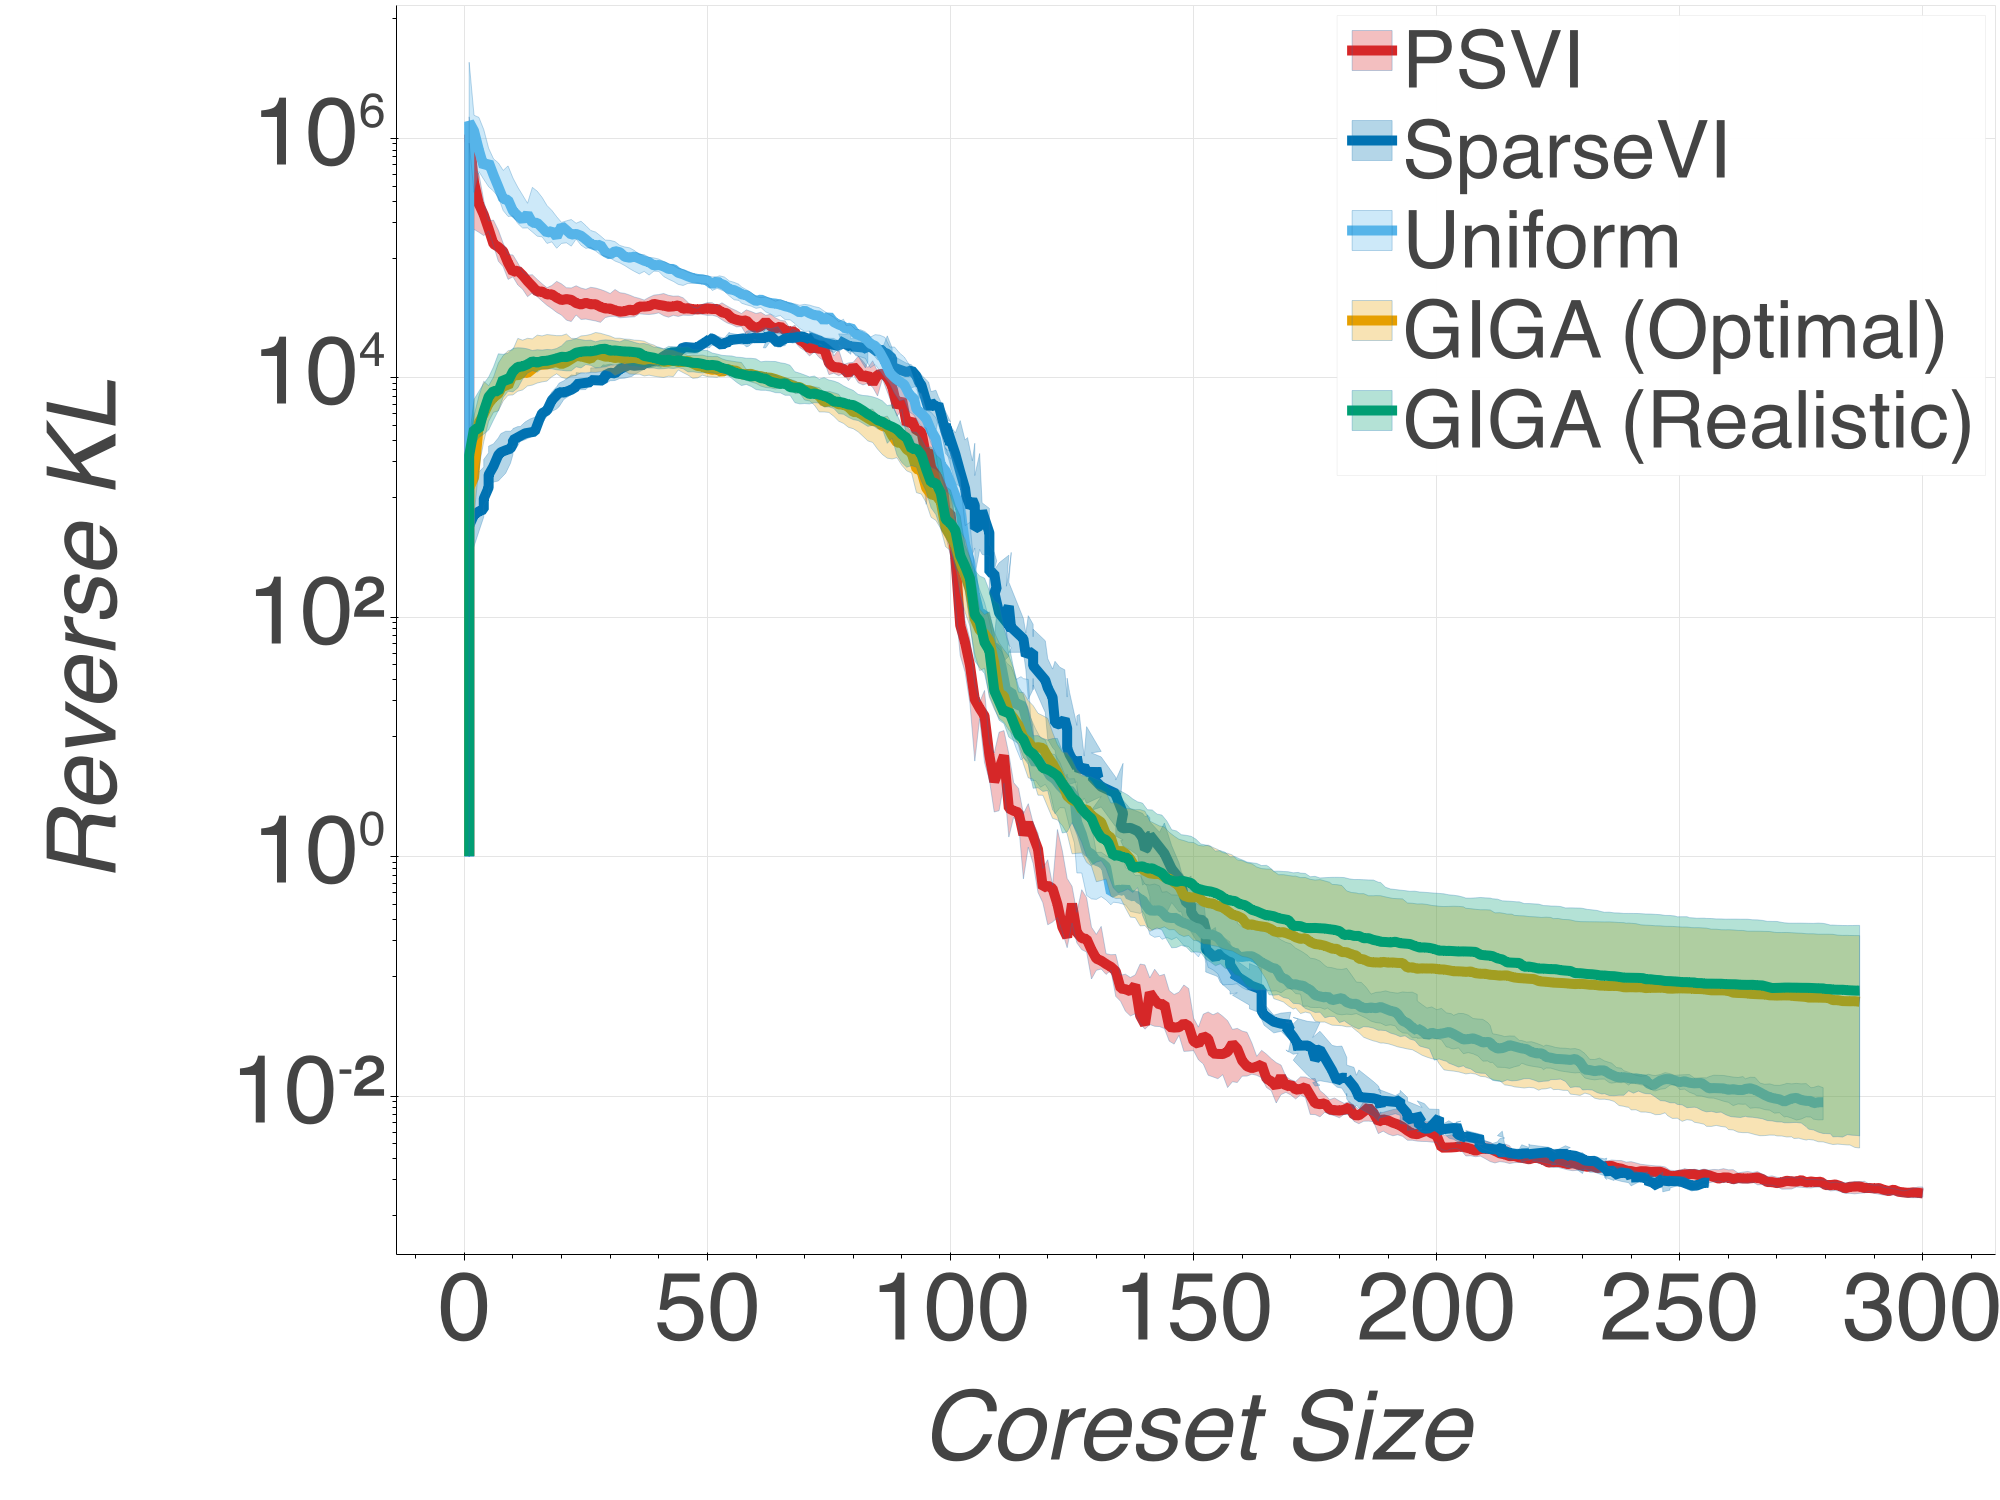
\includegraphics[width=1.15\columnwidth]{\MyPath/figs/linregT__projdim200_KLDvssz.png}}%
			\caption{$\text{project. dim.}=200$}
	\end{subfigure}\hfill\qquad
	\centering
	\begin{subfigure}[b]{.29\textwidth}
		\centerline{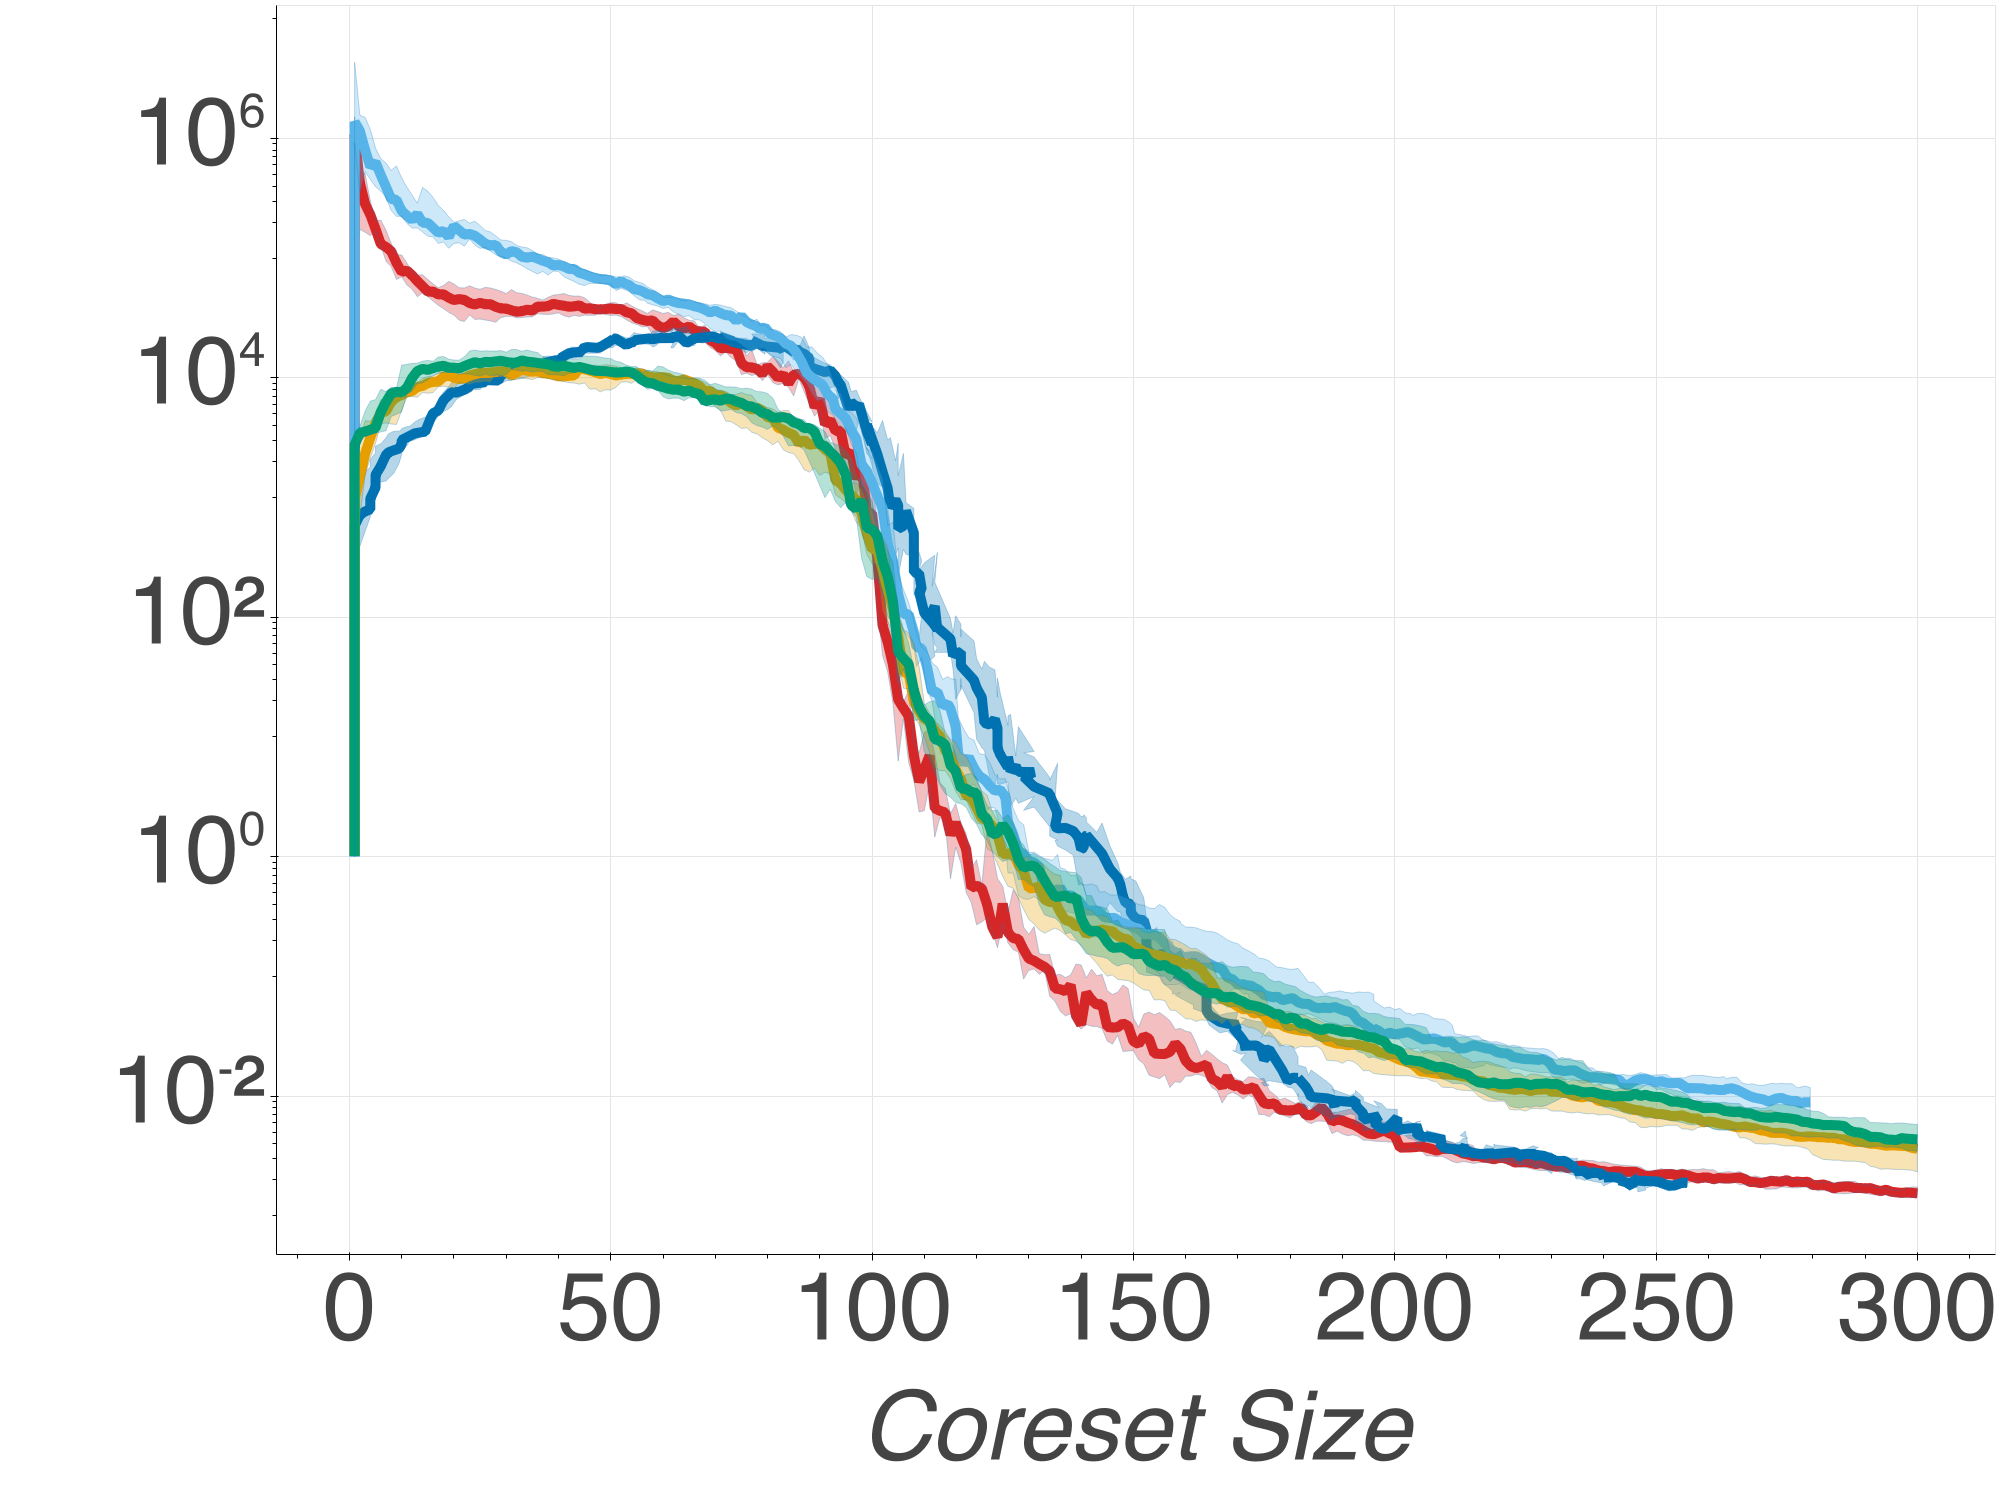
\includegraphics[width=1.15\columnwidth]{\MyPath/figs/linregT__projdim2000_KLDvssz.png}}%
			\caption{$\text{project. dim.}=2,000$}
	\end{subfigure}\hfill\qquad
	\centering
	\begin{subfigure}[b]{.29\textwidth}
		\centerline{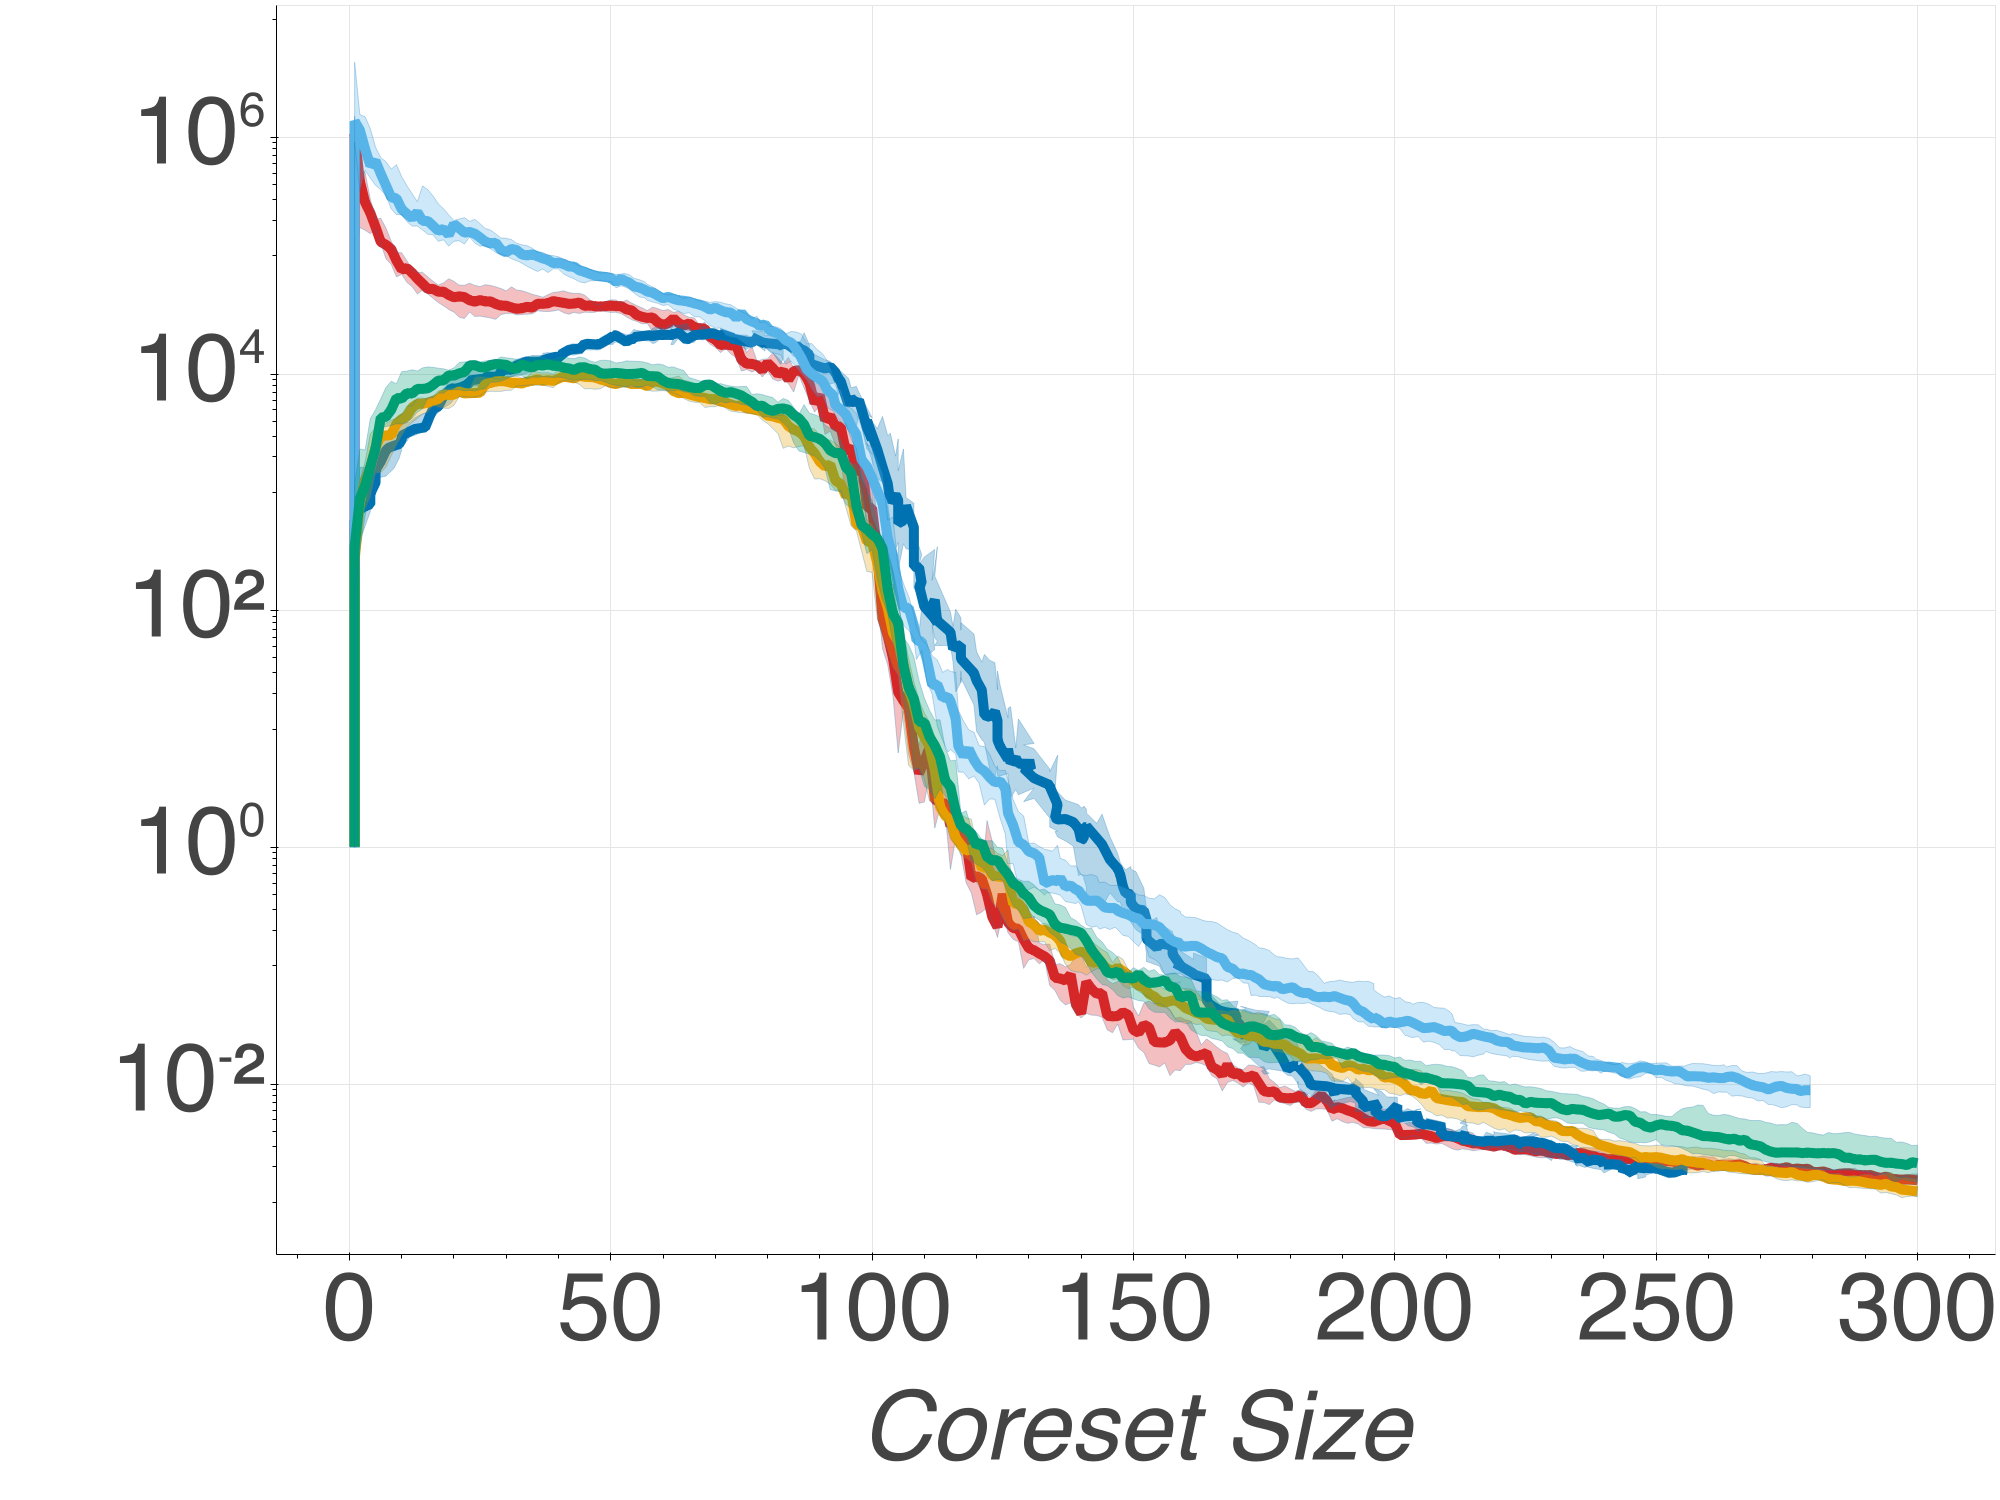
\includegraphics[width=1.15\columnwidth]{\MyPath/figs/linregT__projdim10000_KLDvssz.png}}%
			\caption{$\text{project. dim.}=10,000$}
	\end{subfigure}
	\caption{Comparison of Hilbert coresets performance on Bayesian linear regression experiment for increasing projection dimension (over 10 trials).}
	\label{fig:hilbert_varying_projdim}
\end{figure}

Here we present some more plots demonstating the dependence of Hilbert coresets approximation quality on the number of random dimensions in the Bayesian linear regression setting presented in~\cref{fig:linreg_300}. We remind that dimension used at this experiment and throughout the entire experiments section was set to 100. Increasing this number is typically expensive to obtain in practice. As demonstrated in~\cref{fig:hilbert_varying_projdim}, getting higher projection dimension enables better posterior approximation in the problem, while \gigao~starts offering better quality of approximation than \gigar. However, \psvi~remains competitive in the small coreset regime even for Hilbert coresets with extremely large projection dimensionality, demonstrating the information-geometric limitations that Hilbert coreset constructions are known to face~\cite{campbell19neurips}.



\subsection{Bayesian Logistic Regression}
\label{supp:logreg_experiment_appendix}
 

\subsubsection{Model}
\label{supp:logreg_model_appendix}
In logistic regression we have a set of datapoints $(x_n, y_n)_{n=1}^{N}$ each corresponding to a feature vector ${x_n \in \reals^d}$ and a label ${y_n \in \{-1, 1\}}$. Datapoints are assumed to be generated according to following statistical model
\[
y_n | x_n, \theta \sim \distBern \left( \frac{1}{1+e^{-z_n \theta}} \right) 
\quad 
z_n := \begin{bmatrix}
			x_n \\
			1
		\end{bmatrix}.
\label{eq:logreg-model}
\]
The aim of inference is to compute the posterior over the latent parameter $ \theta = [\theta_0 \ldots \theta_d]^T \in \reals^{d+1}$.
Log-likelihood of each datapoint can be expressed as
\[
\begin{split}
f_n(x_n, y_n|\theta)  
=&\ind{[y_n=-1]}\log \left( 1 - \frac{1}{1+e^{-z_n^T \theta}}\right) 
- \ind{[y_n=1]} \log \left( 1+ e^{-z_n^T \theta}  \right) \\
=&-\log\left( 1 + \exp(-y_n z_n^T\theta)\right).
\label{eq:logreg-loglik}
\end{split}
\]
Hence in pseudocoreset construction we can optimize pseudodata point locations with respect to continuous variable $ x_n$, using the gradient
\[
\nabla_{x_n}f_n =  \frac{e^{-y_n z_n^T \theta}}{1+e^{-y_n z_n^T \theta}}y_n \begin{bmatrix}
\theta_1 \\
\vdots \\
\theta_d
\end{bmatrix}.
\label{eq:logreg-loglik-locgrad}
\]



\subsubsection{Datasets description}
\label{supp:logreg_data_details}
For logistic regression experiments, we used subsampled and full versions of datasets presented in~\cref{table:datasets_details}: a synthetic dataset with $ x\in \reals^2 $ sampled \iid from a $\distNorm{(0, I)}$ and $ y\in\{-1,1\} $ sampled from respective logistic likelihood with $ \theta =[3, 3, 0]^T$ (\textsc{Synthetic}); a phishing websites dataset reduced to $ D=10 $ via PCA (\textsc{Phishing}); a chemical reactivity dataset with  real-valued features corresponding to its first $ 10 $ and $ 100 $ principal components (\textsc{ChemReact} and \textsc{ChemReact100} respectively); a dataset with $ 50 $ real-valued features associated with whether each of $ 100K $ customers of a bank will make a specific transaction (\textsc{Transactions}); and a dataset for music analysis, where we consider "classical vs all" genre classification task (\textsc{Music}). Original versions of the four latter datasets are available online respectively at~\href{https://www.csie.ntu.edu.tw/~cjlin/libsvmtools/datasets/binary.html}{https://www.csie.ntu.edu.tw/\~{}cjlin/libsvm tools/datasets/binary.html},  \href{http://komarix.org/ac/ds/}{http://komarix.org/ac/ds},  \href{https://www.kaggle.com/c/santander-customer-transaction-prediction/data}{https://www.kaggle.com/c/santander-customer- transaction-prediction/data}, and \href{https://github.com/mdeff/fma}{https://github.com/mdeff/fma}. 

\begin{table}[!h]
	\begin{center}
		\begin{tabular}{|l|l|l|}
			\hline
			\textbf{Dataset name}       & $N$      & $D$   \\ \hline
			\textsc{Synthetic}  & 500    & 2   \\ \hline
			\textsc{Phishing}   & 500    & 10  \\ \hline
			\textsc{ChemReact}        & 500    & 10  \\ \hline
			\textsc{Transactions}  & 100,000   & 50   \\ \hline
			\textsc{ChemReact100}    & 26,733 & 100 \\ \hline
			%mnist      & 10,000    & 758 \\ \hline
		    \textsc{Music}      & 8,419    & 237 \\ \hline
		\end{tabular}
	\end{center}
	\caption{Details for datasets used in logistic regression experiments.}
	\label{table:datasets_details}
\end{table}

\subsubsection{Small-scale experiments}
\label{supp:small_scale_appendix}
In the small-scale experiment, the number of overall gradient updates was
set to $T = 1,500$, while minibatch size was set to  $B = 400$. Learning rate schedule for \sparsevi~and \psvi~was ${\gamma_t = 0.1t^{-1}}$. Results presented in~\cref{fig:smallscale_ls_blogreg_dkl} indicate that~\psvi~achieves superior quality to~\sparsevi~for small coreset sizes, and is competitive to~\gigao, while the latter unrealistically uses true posterior samples to tune a weighting function required over construction.


\begin{figure*}[!t]
	\centering
	\begin{subfigure}[b]{.29\textwidth}
		\caption*{\textsc{Synthetic}}
		\vspace*{-0.3cm}
		\centerline{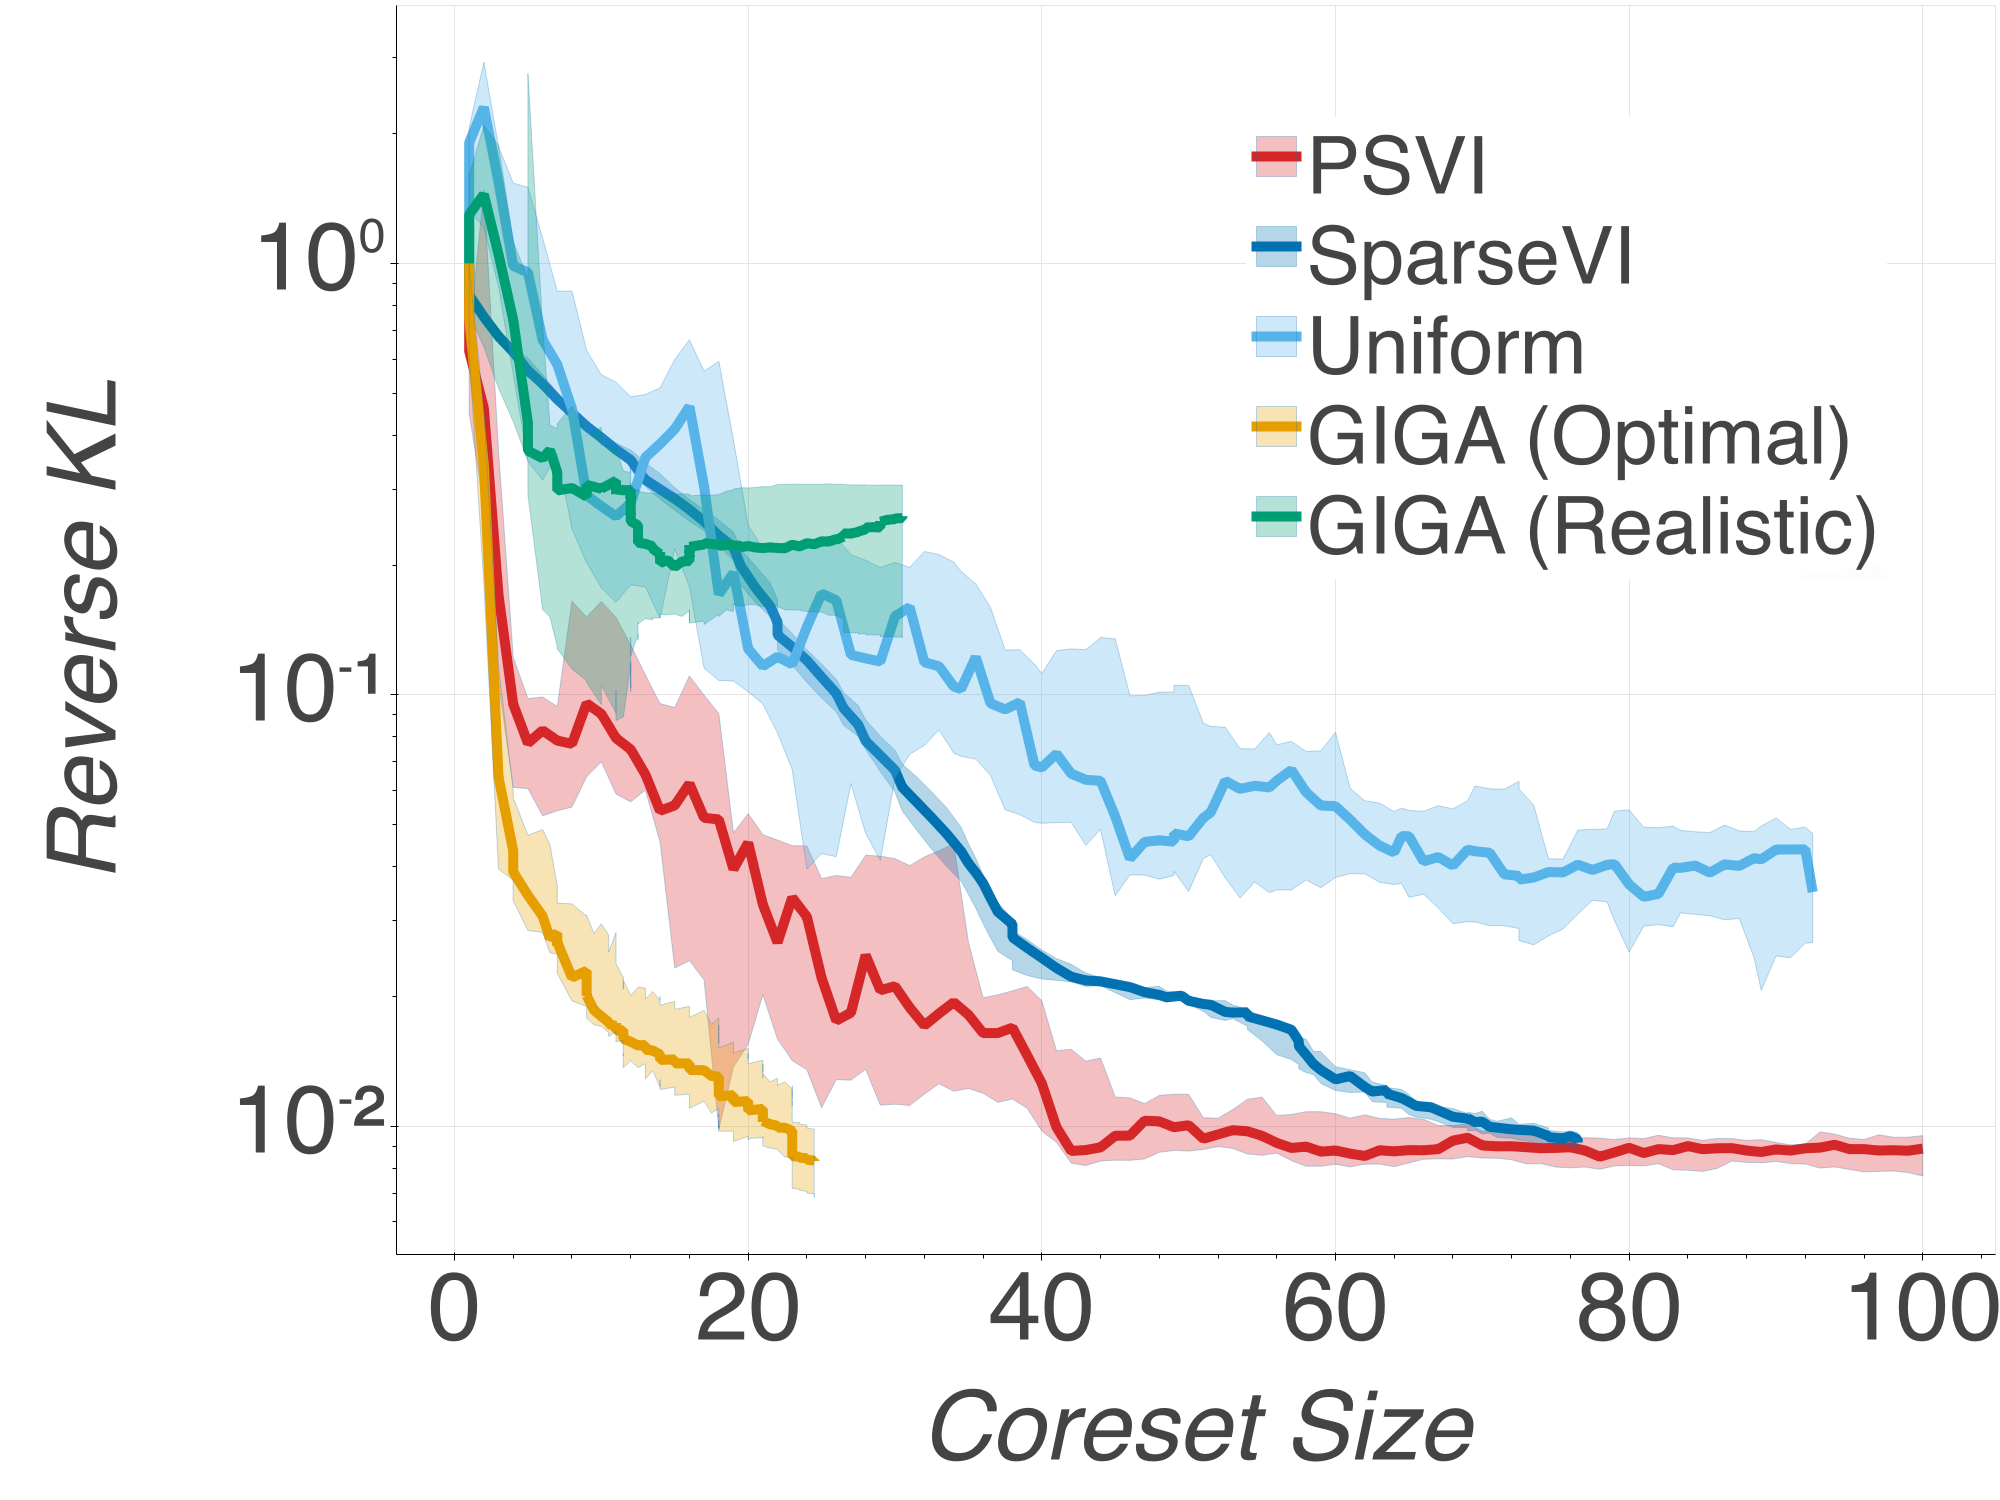
\includegraphics[width=1.15\columnwidth]{\MyPath/figs/synth_lr_KLDvssz.png}}%
	\end{subfigure}\hfill\qquad
	\centering
	\begin{subfigure}[b]{.29\textwidth}
		\caption*{\textsc{Phishing}}
		\vspace*{-0.3cm}
		\centerline{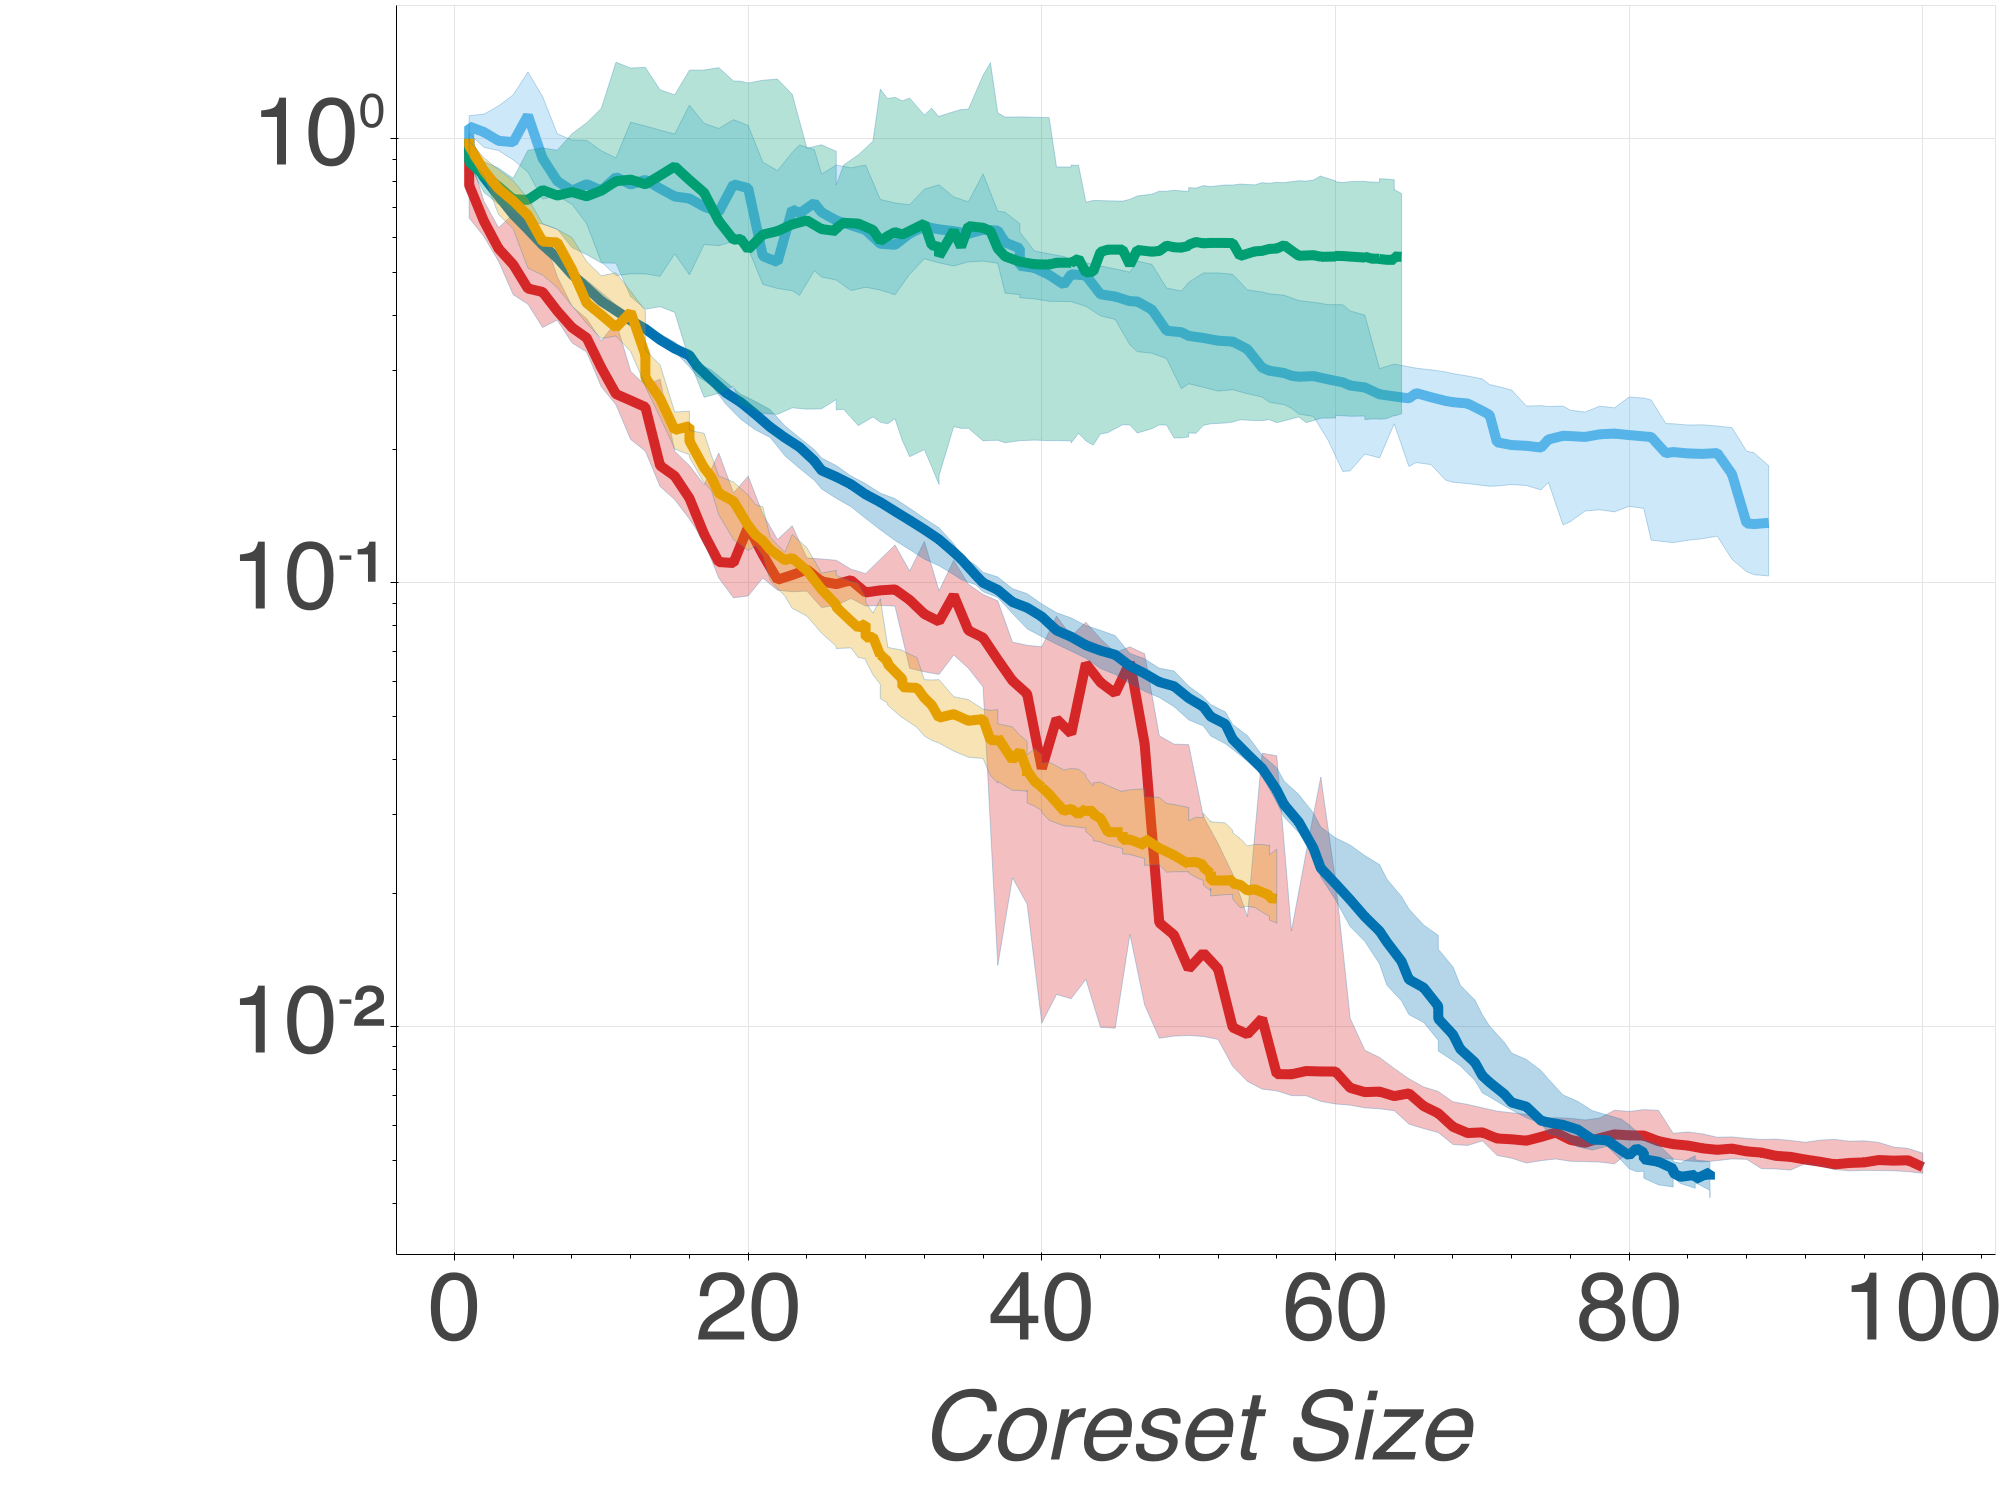
\includegraphics[width=1.15\columnwidth]{\MyPath/figs/phishing_KLDvssz.png}}%
	\end{subfigure}\hfill\qquad
	\centering
	\begin{subfigure}[b]{.29\textwidth}
		\caption*{\textsc{ChemReact}}
		\vspace*{-0.3cm}
		\centerline{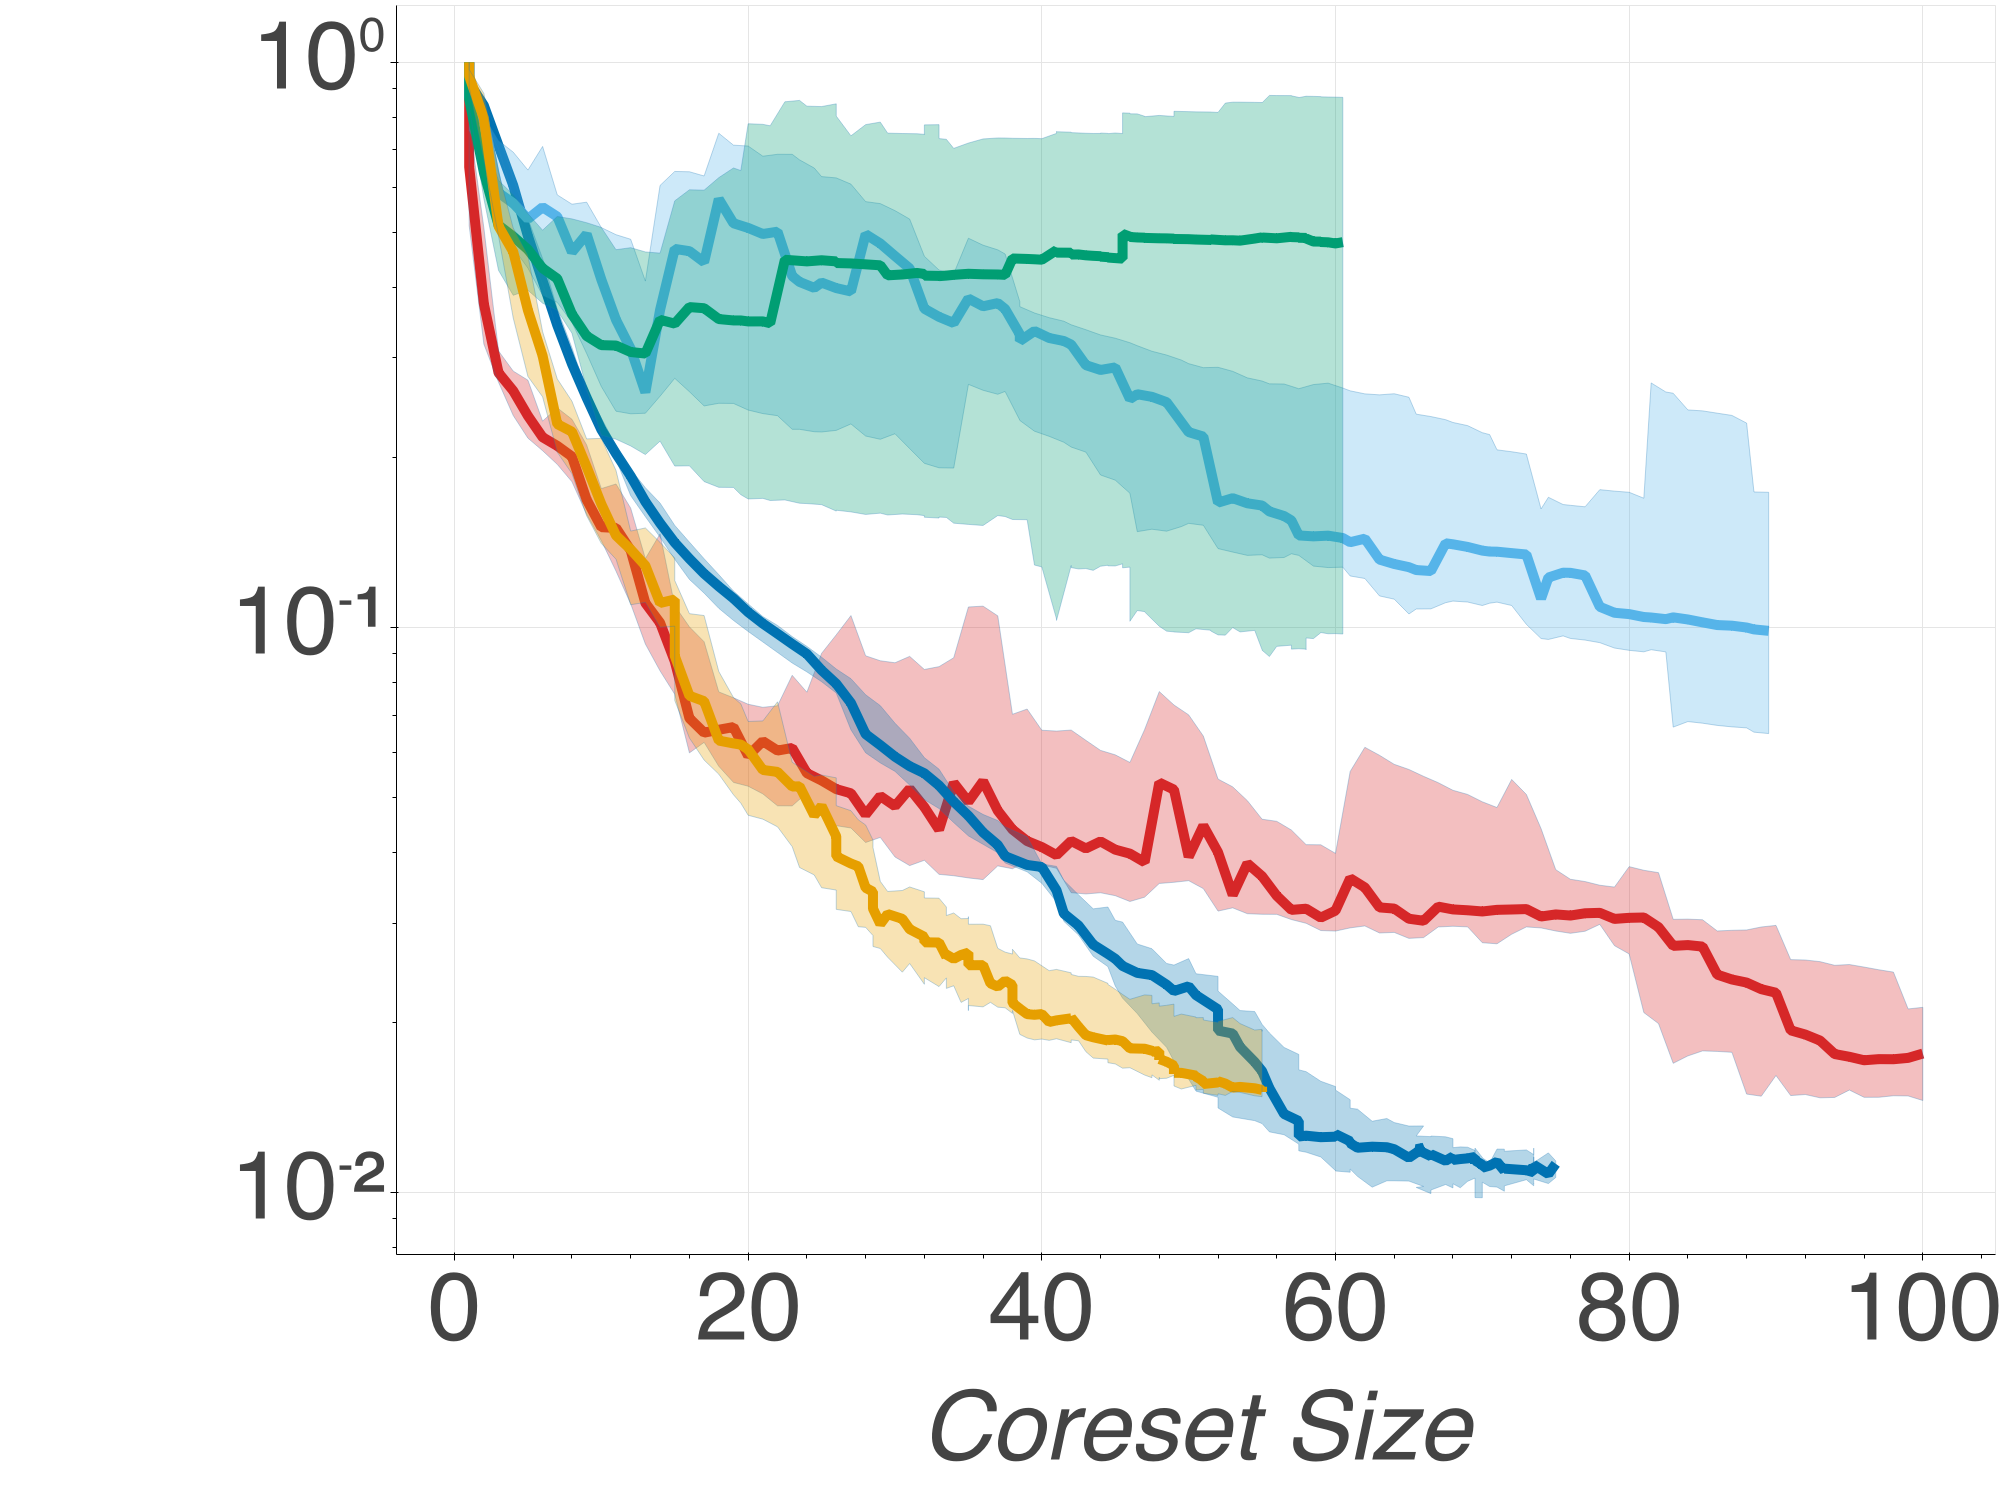
\includegraphics[width=1.15\columnwidth]{\MyPath/figs/ds1_KLDvssz.png}}%
	\end{subfigure}
	\caption{Comparison of (pseudo)coreset approximate posterior
	quality vs  coreset
	size for logistic regression over 10 trials.}
\label{fig:smallscale_ls_blogreg_dkl}
\end{figure*}

\subsubsection{Reproducibility of Bayesian Logistic Regression experiment}
\label{supp:reproducibility}
In this subsection we provide additional details for reproducibility of the experimental setup for the Bayesian Logistic Regression experiment presented in~\cref{sec:experiments}.  

\paragraph{Posterior approximation metrics, coreset gradients and learning rates} Posterior approximation quality was estimated via computing KL divergence between Gaussian distributions fitted on coreset and full data posteriors via Laplace approximation. For both \sparsevi~and \psvi, gradients were estimated using samples drawn from a Laplace approximation fitted on current coreset weights
and points. To optimize initial learning rates for \sparsevi~and \psvi, we did a grid search over ${\{0.1, 1, 10\}}$.

\paragraph{Differential privacy loss accounting and hyperparameter selection}  In the differential privacy experiment, we were not concerned with the extra privacy cost of hyperparameter optimization task.  Estimation of differential privacy cost at all experiments was based on TensorFlow privacy implementation of moments accountant for the subsampled Gaussian mechanism\footnote{\href{https://github.com/tensorflow/privacy}{https://github.com/tensorflow/privacy}}. 
For \dpsvi~we used the best learning hyperparameters found for \psvi~on the corresponding dataset. The demonstrated range of privacy budgets was generated by decreasing the variance $ \sigma $ of additive Gaussian noise and keeping the rest of hyperparameters involved in privacy accounting fixed.  
Regarding \dpvi, over our experiments we also kept subsampling ratio fixed. We based our implementation of \dpvi~on authors code,\footnote{\href{https://github.com/DPBayes/DPVI-code}{https://github.com/DPBayes/DPVI-code}} adapting noise calibration according to the adjacency relation used in~\cref{sec:dp-pseudocoresets}, and the standard differential privacy definition~\citep{dwork14}. In our experiment, we used the AdaGrad optimizer~\citep{duchi11}, with learning rate $0.01$, number of iterations $2,000$, and minibatch size $200$. Gradient clipping values for \dpvi~results presented in~\cref{fig:dklvseps}, for \textsc{Transactions}, \textsc{ChemReact100}, and \textsc{Music} datasets were tuned via grid search over ${\{1, 5, 10, 50\}}$. The values of gradient clipping constant giving best privacy profiles for each dataset, used in~\cref{fig:dklvseps}, were 10, 5, and 5 respectively. 



\subsubsection{Additional Plots}
\label{supp:cpu_timings}



\begin{figure*}[!t]
	\centering
	\begin{subfigure}[b]{.29\textwidth}
		\caption*{\textsc{Synthetic}}
		\vspace*{-0.3cm}
		\centerline{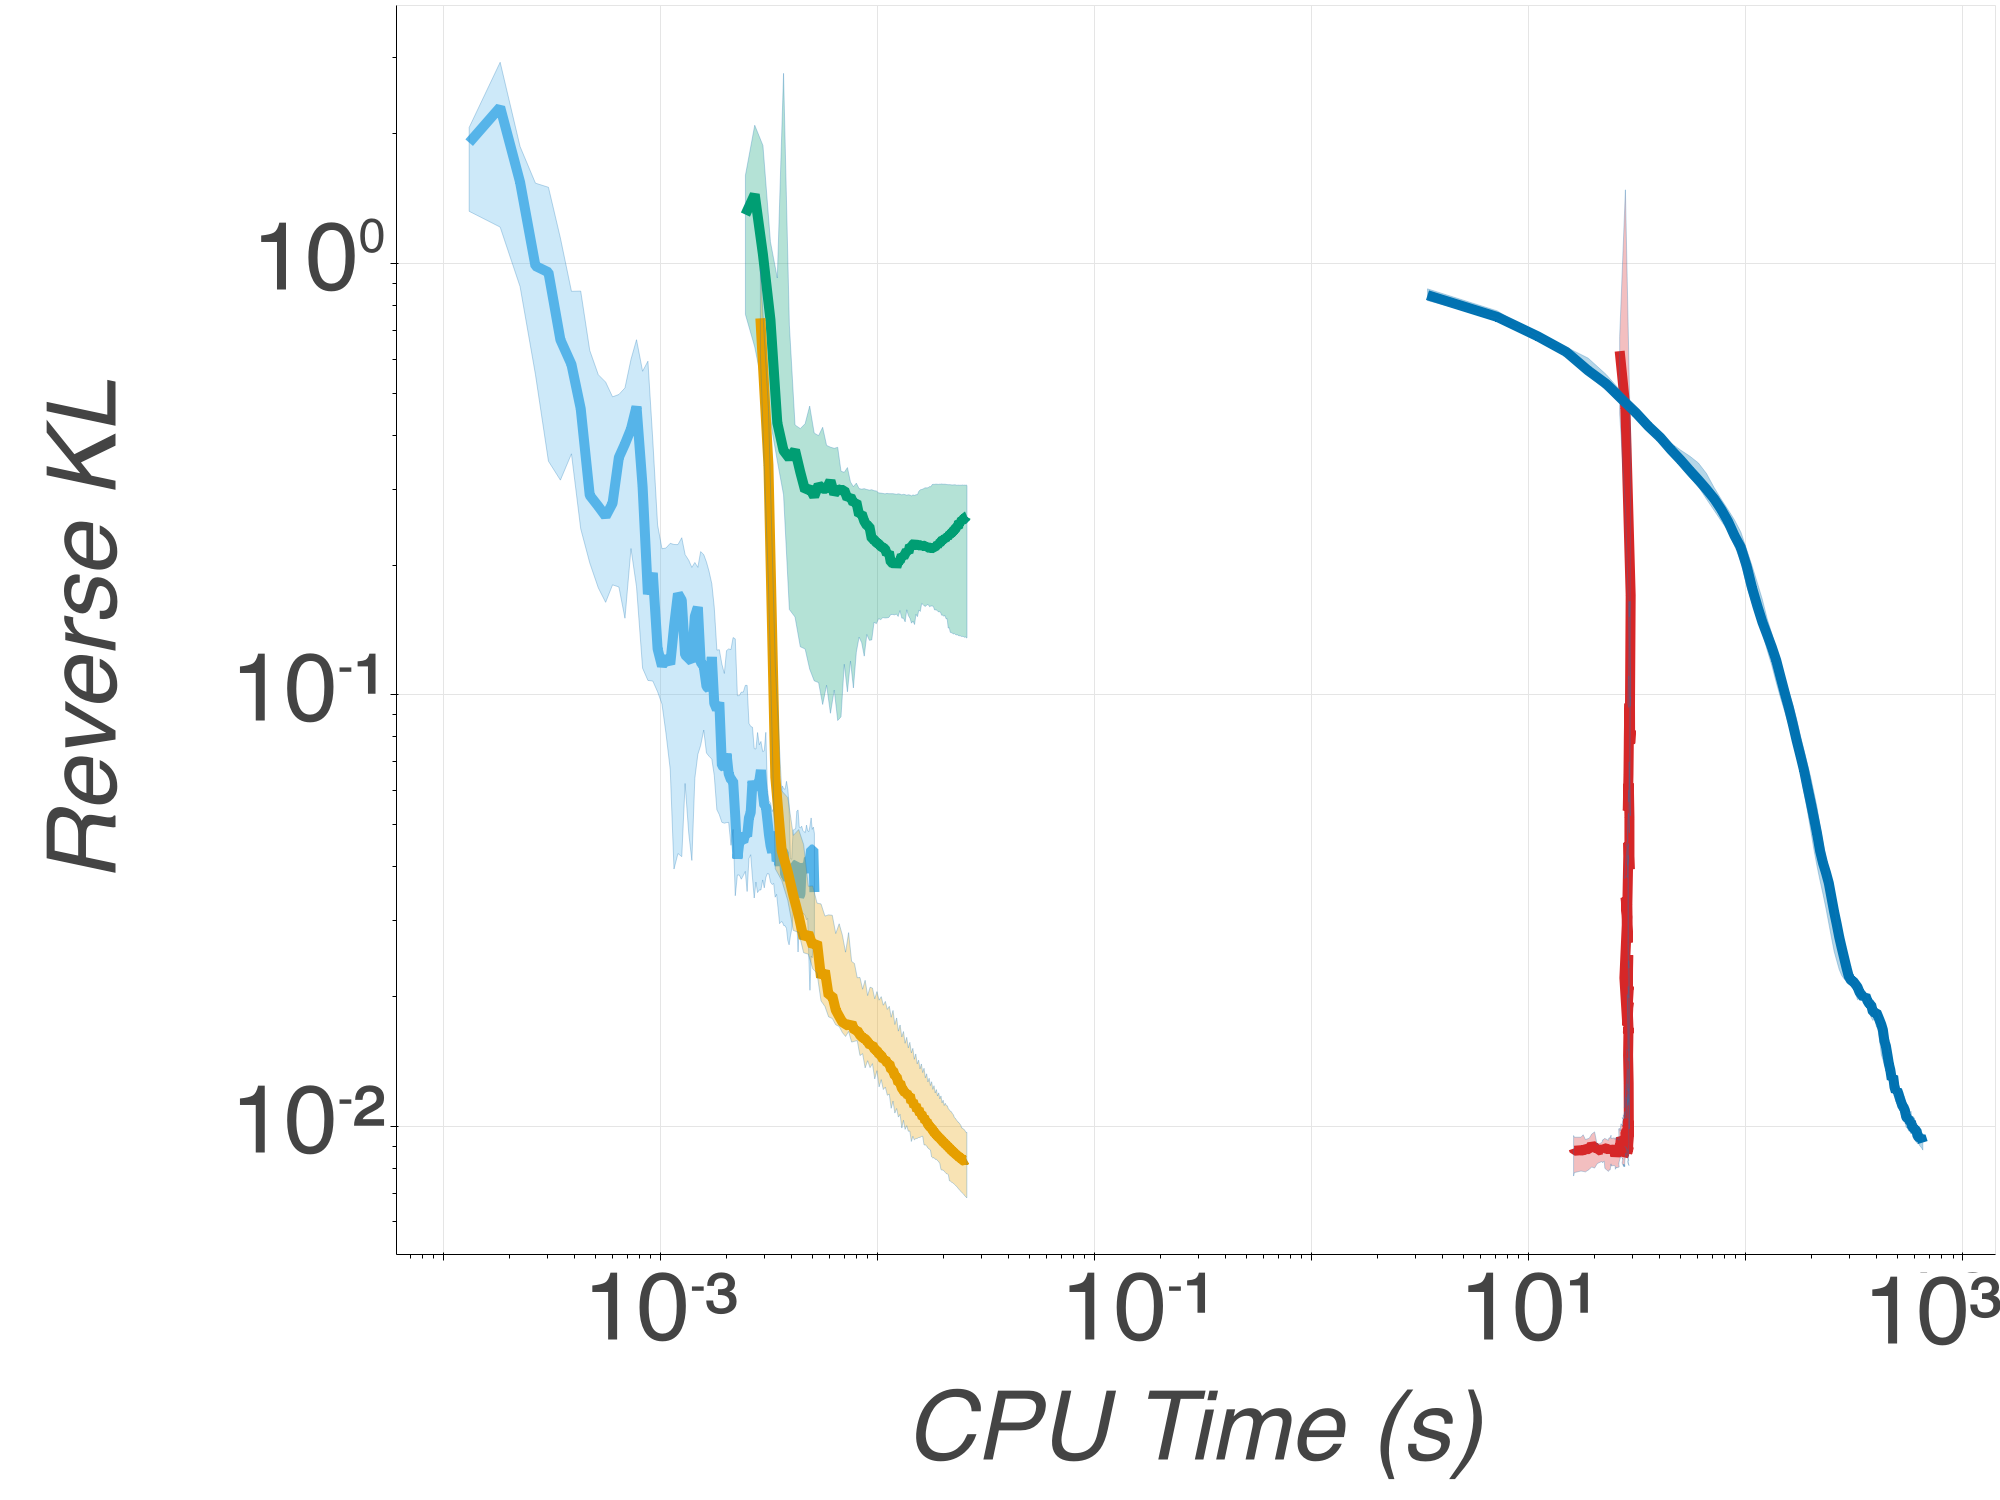
\includegraphics[width=1.15\columnwidth]{\MyPath/figs/synth_lr_KLDvscput.png}}%
	\end{subfigure}\hfill\qquad
	\centering
	\begin{subfigure}[b]{.29\textwidth}
		\caption*{\textsc{Phishing}}
		\vspace*{-0.3cm}
		\centerline{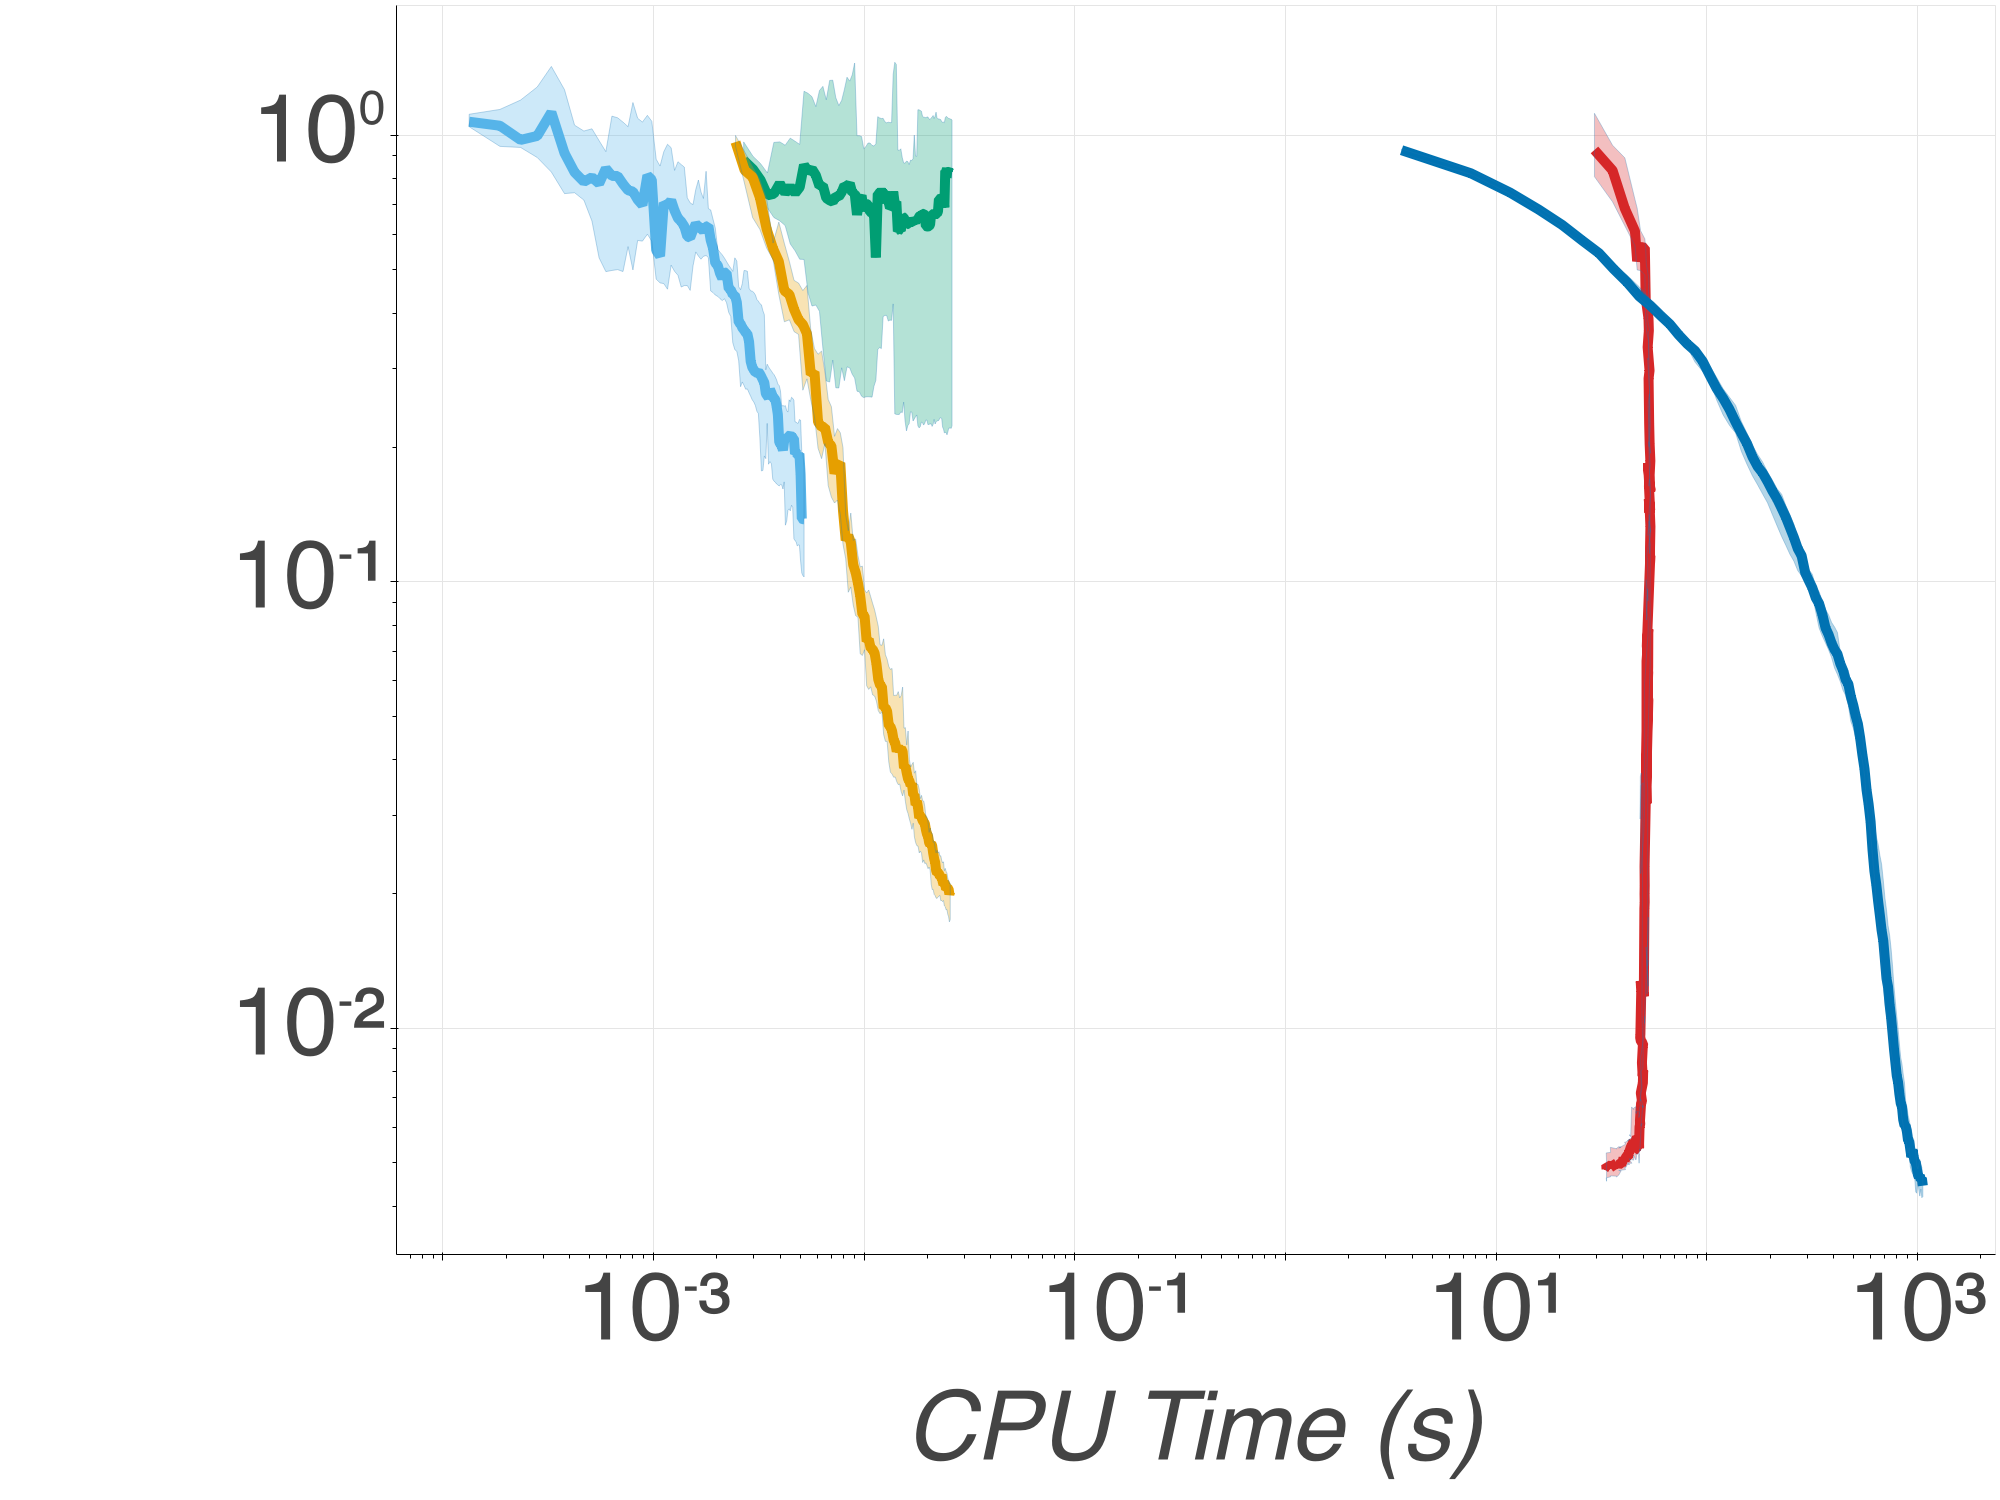
\includegraphics[width=1.15\columnwidth]{\MyPath/figs/phishing_KLDvscput.png}}%
	\end{subfigure}\hfill\qquad
	\centering
	\begin{subfigure}[b]{.29\textwidth}
		\caption*{\textsc{ChemReact}}
		\vspace*{-0.3cm}
		\centerline{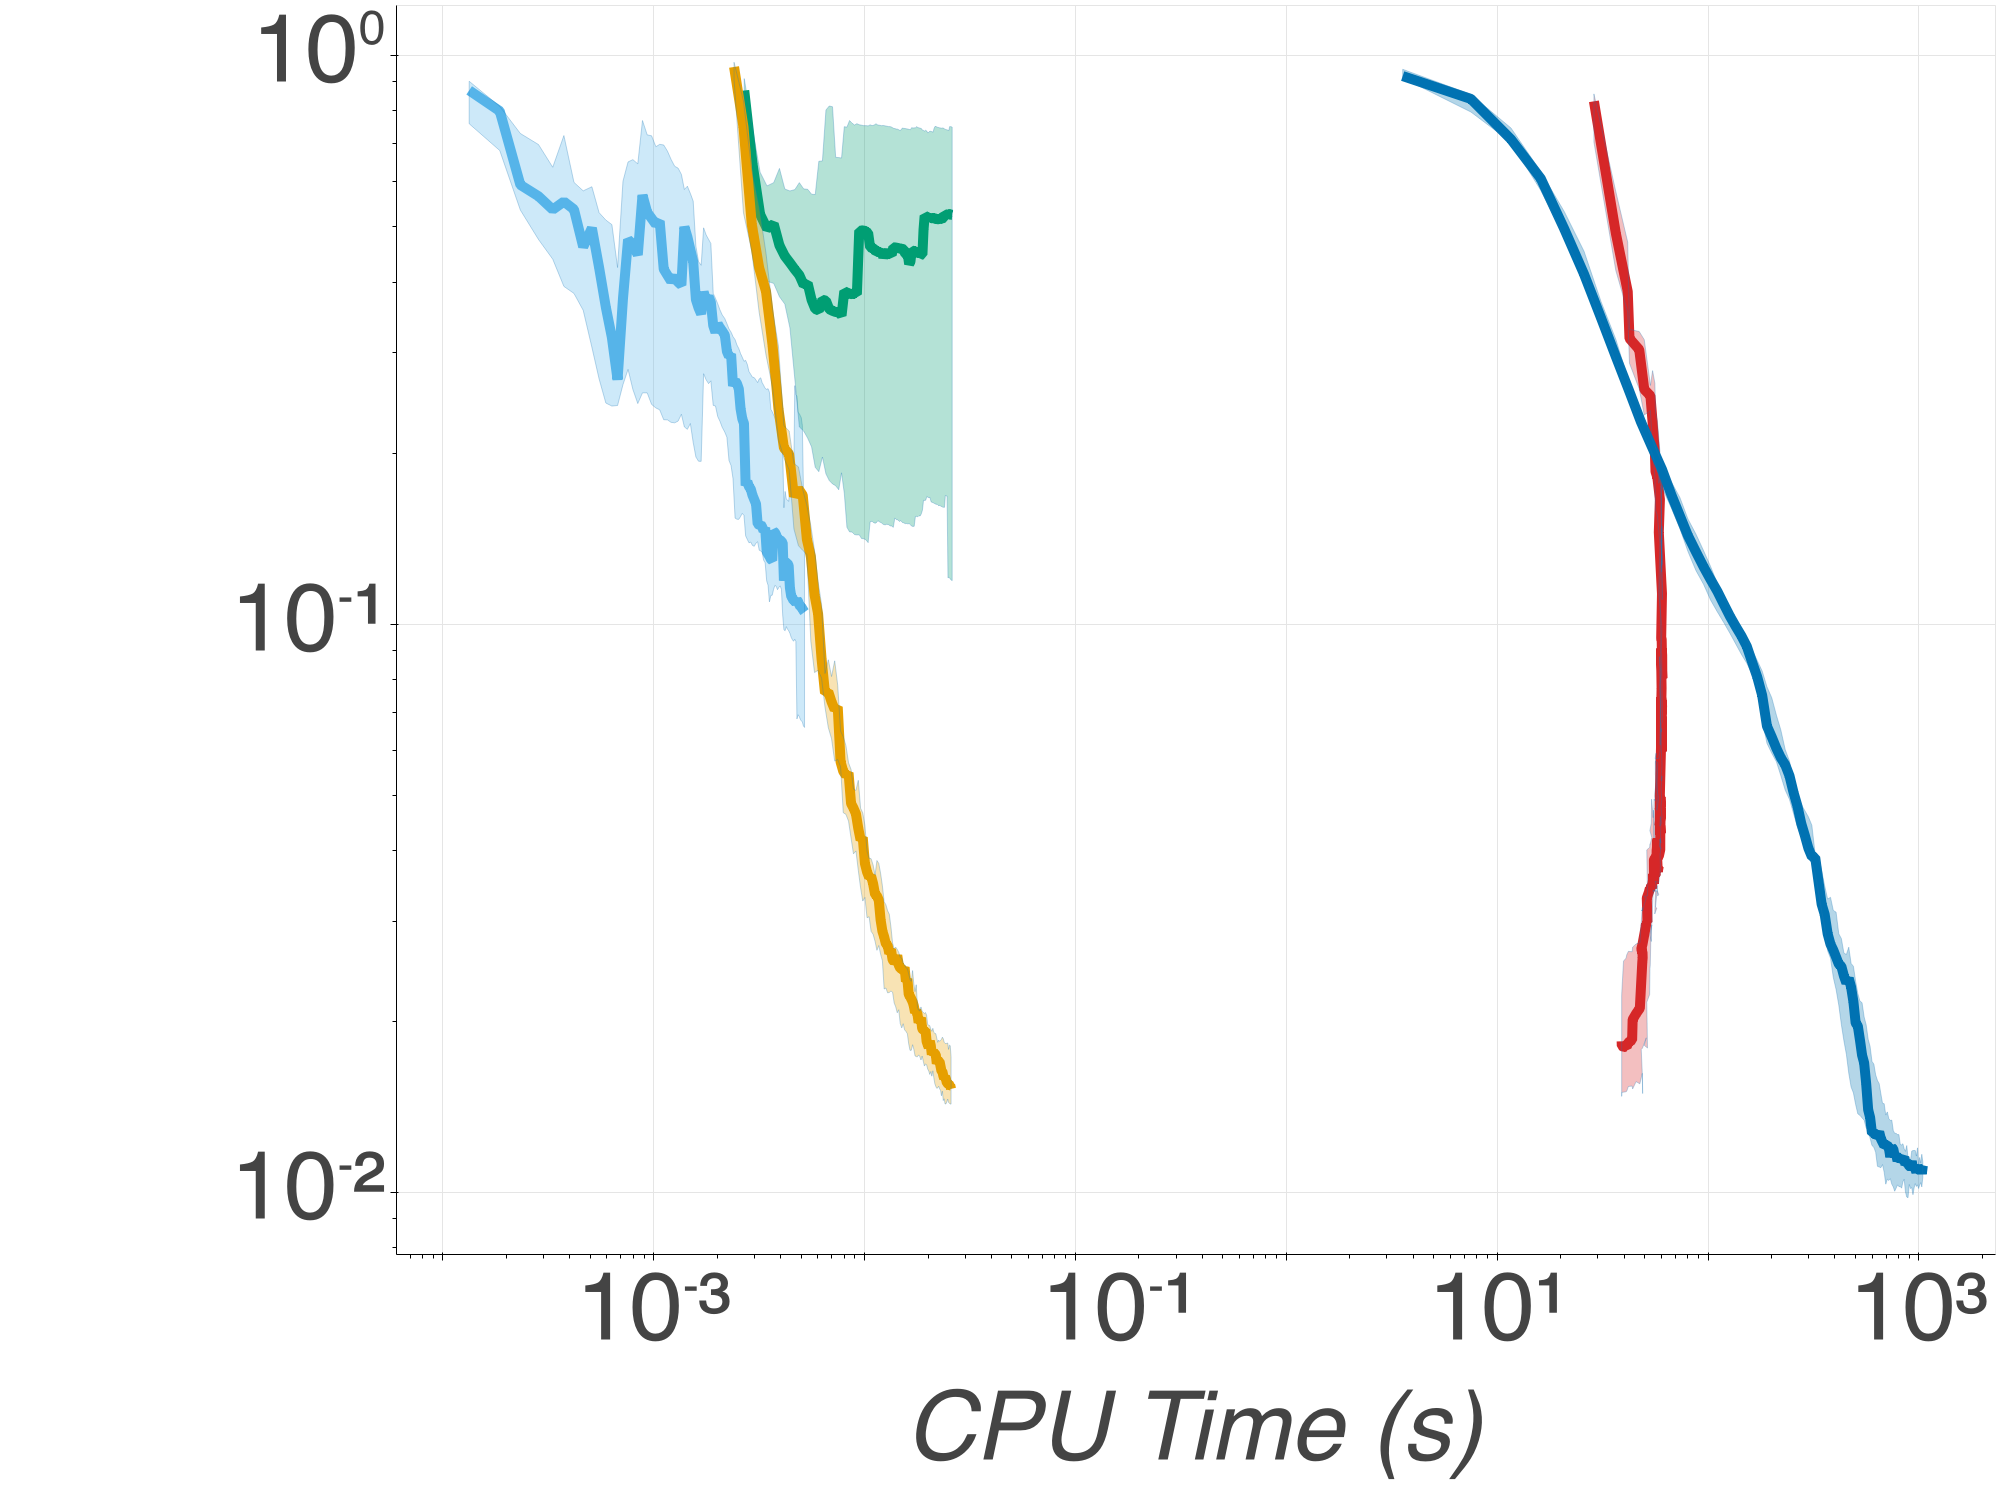
\includegraphics[width=1.15\columnwidth]{\MyPath/figs/ds1_KLDvscput.png}}%
	\end{subfigure}\hfill\qquad
	\centering
	\begin{subfigure}[b]{.29\textwidth}
		\caption*{\textsc{Transactions}}
		\vspace*{-0.3cm}
		\centerline{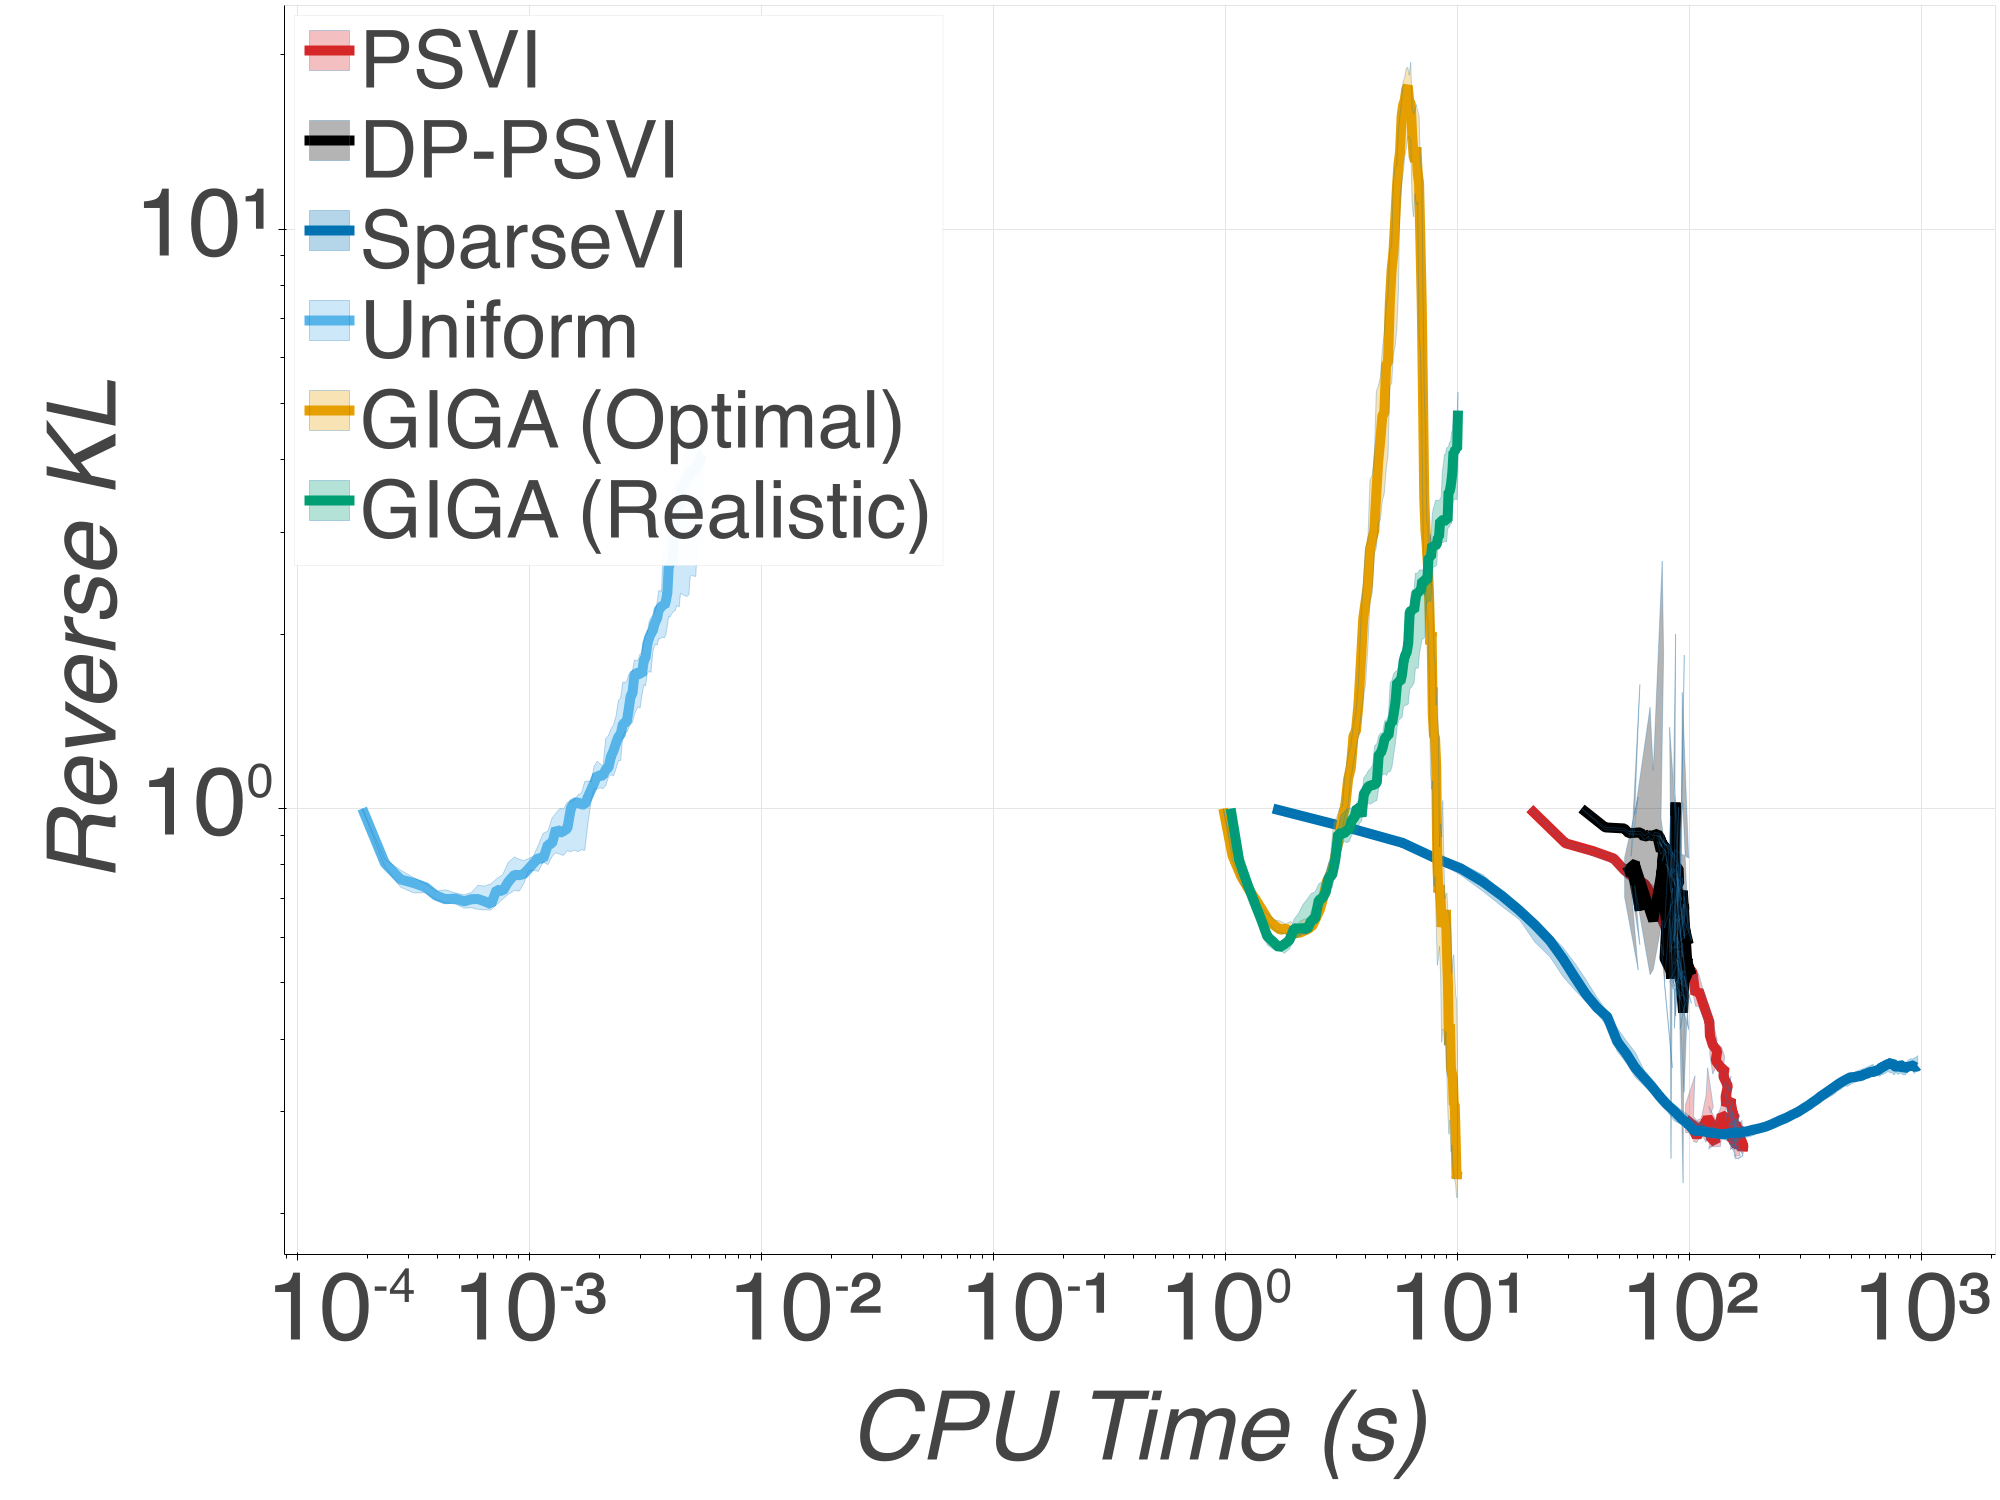
\includegraphics[width=1.15\columnwidth]{\MyPath/figs/wsanta100K_KLDvscput.png}}%
	\end{subfigure}\hfill\qquad
	\centering
	\begin{subfigure}[b]{.29\textwidth}
		\caption*{\textsc{ChemReact100}}
		\vspace*{-0.3cm}
		\centerline{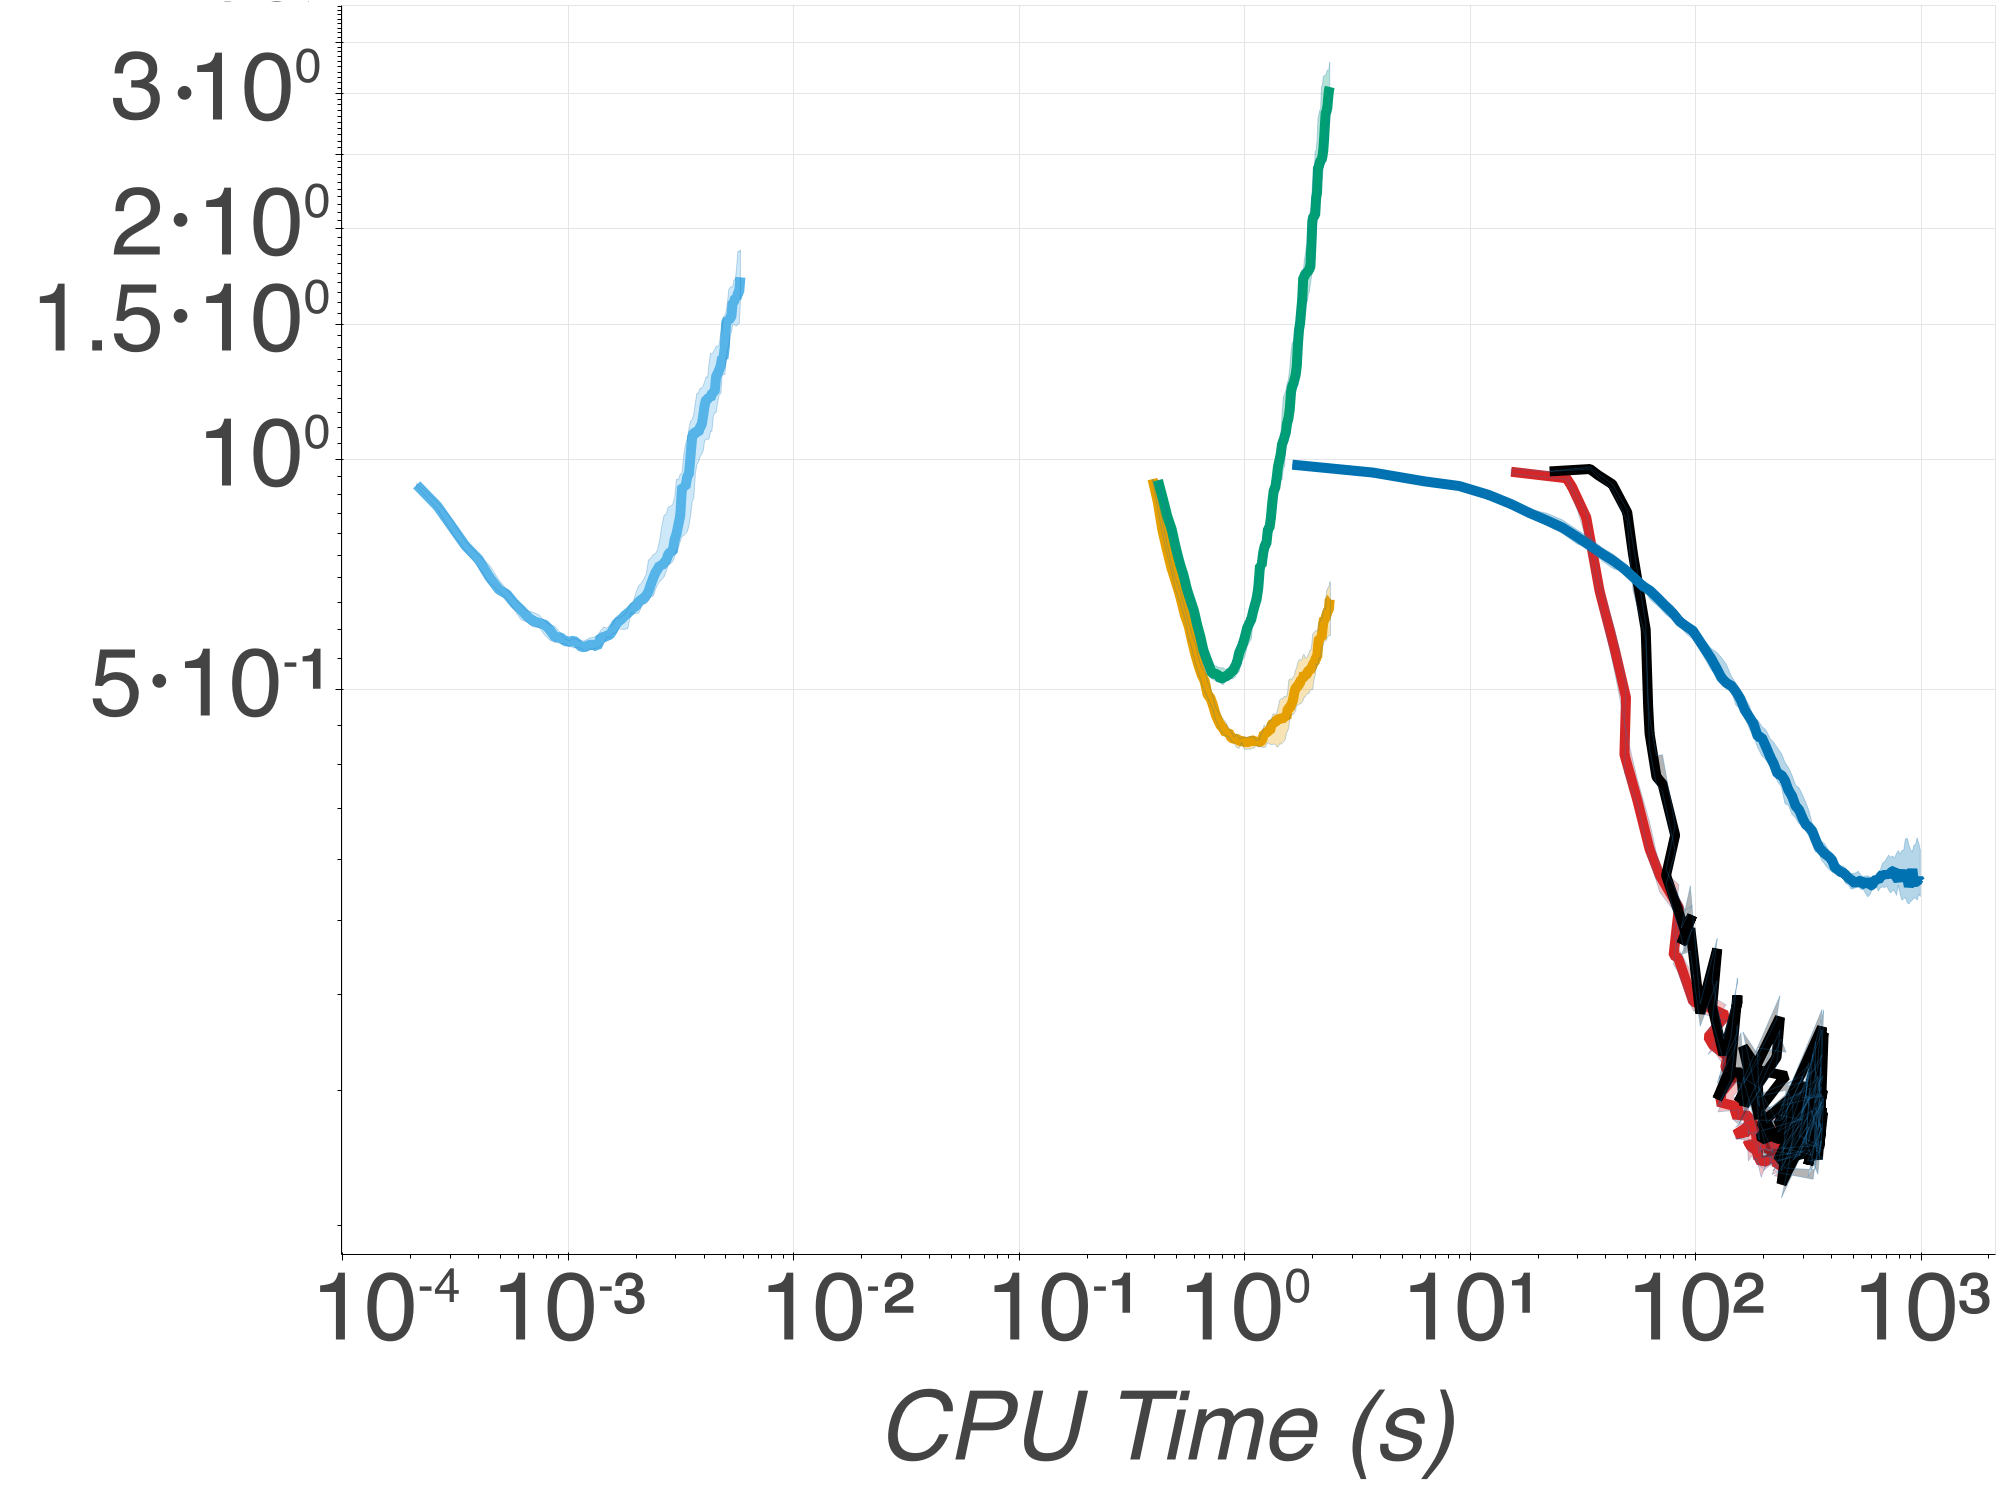
\includegraphics[width=1.15\columnwidth]{\MyPath/figs/wds1100_KLDvscput.png}}%
	\end{subfigure}\hfill\qquad
	\centering
	\begin{subfigure}[b]{.29\textwidth}
		\caption*{\textsc{Music}}
		\vspace*{-0.3cm}
		\centerline{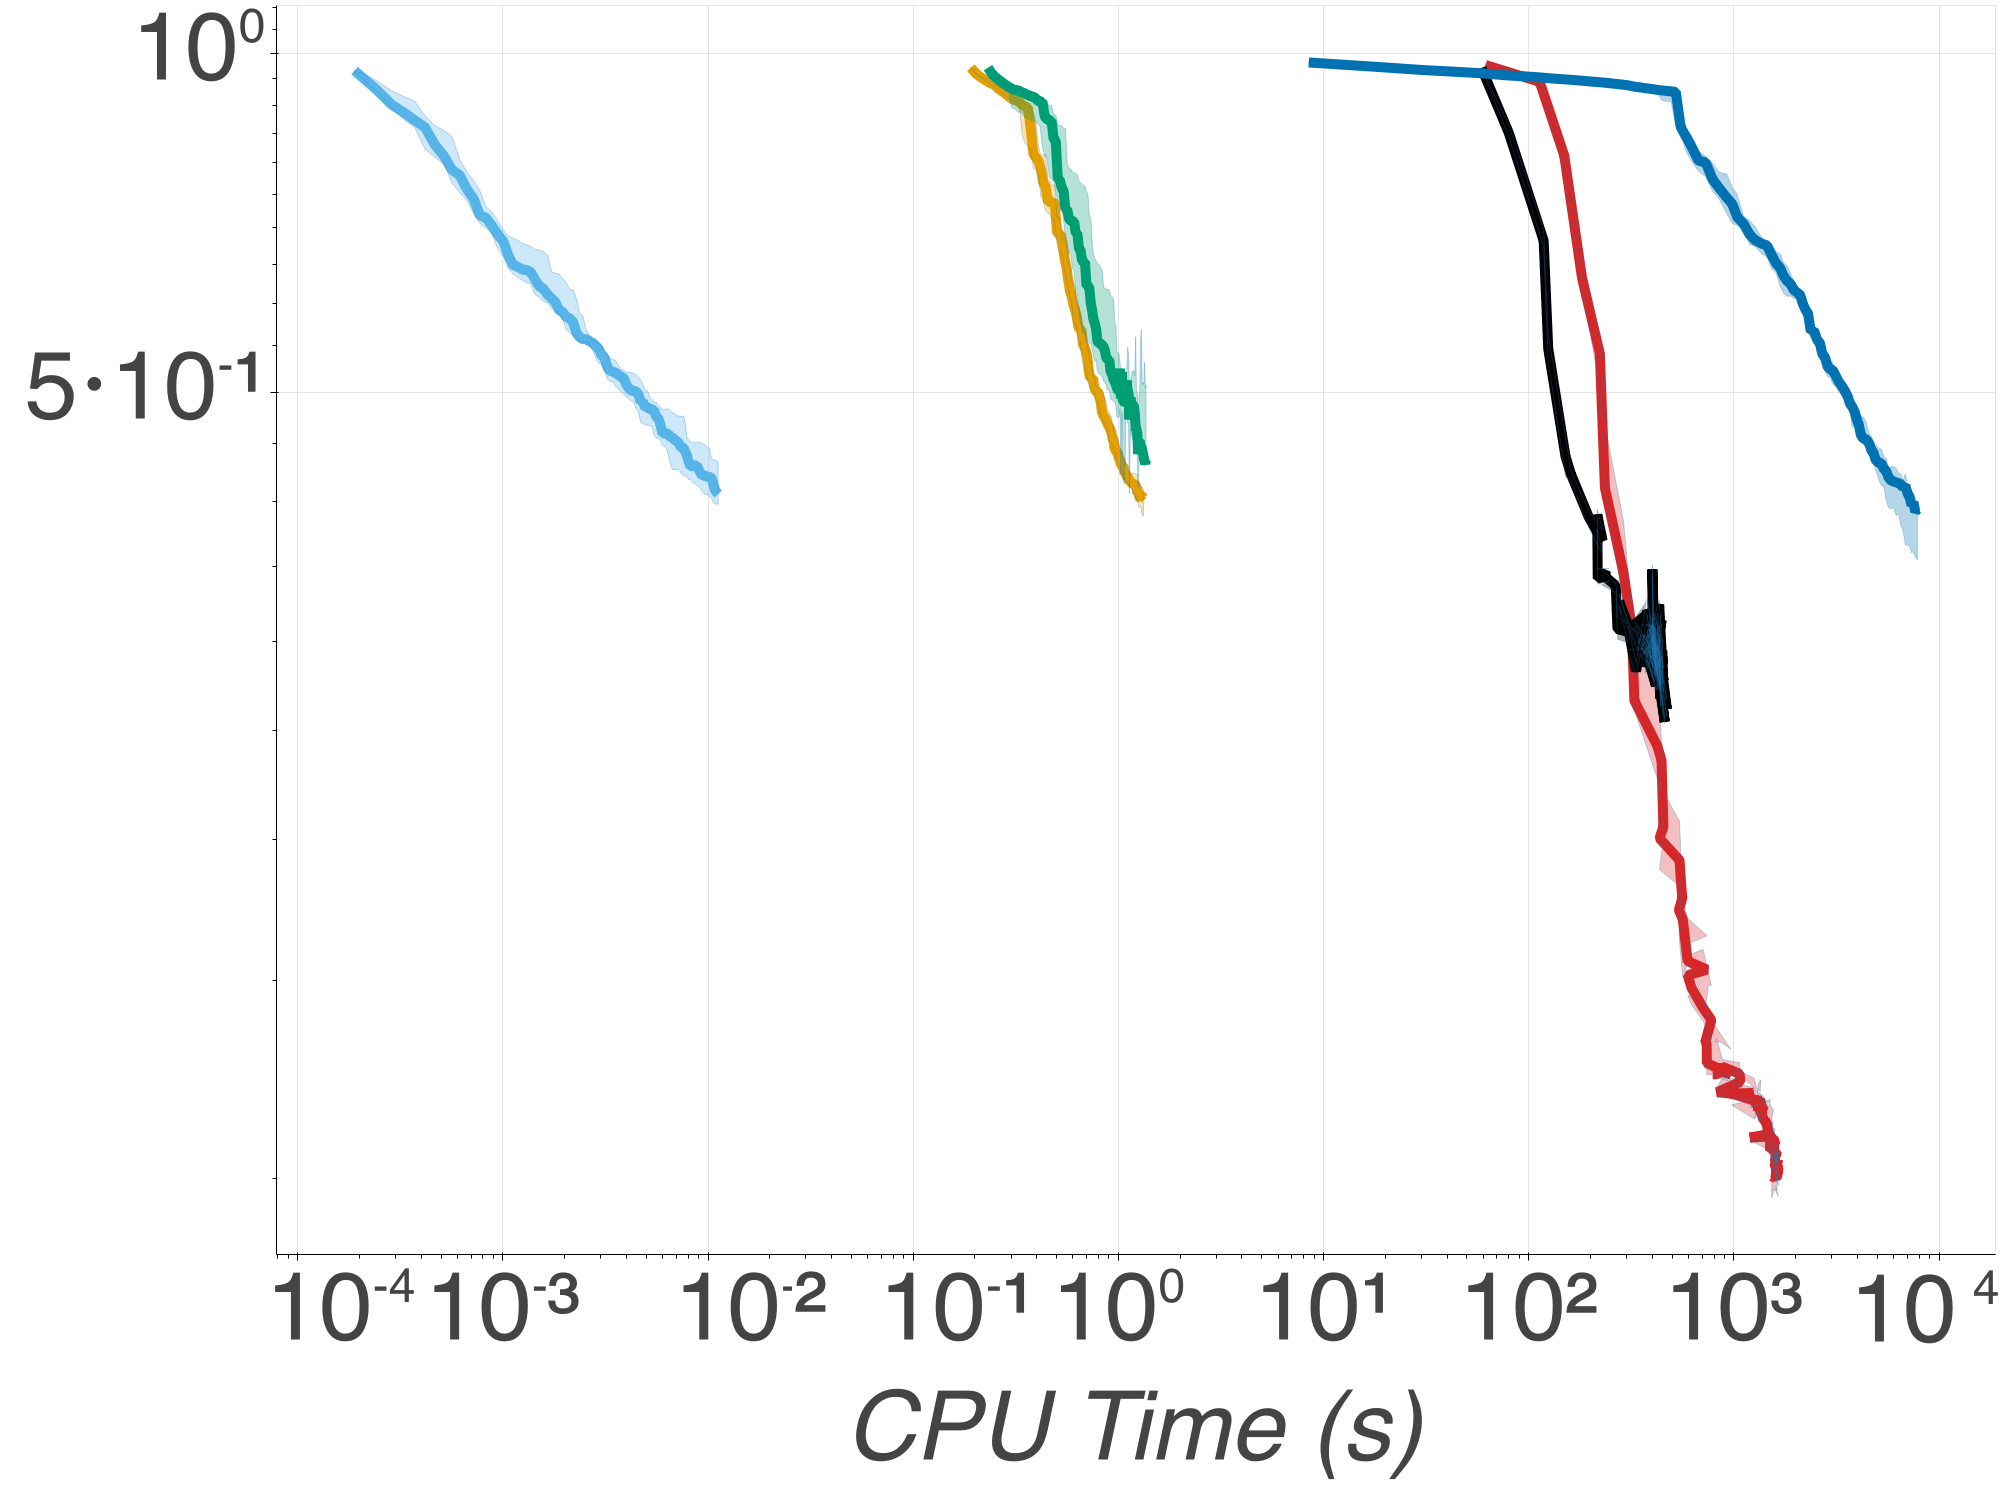
\includegraphics[width=1.15\columnwidth]{\MyPath/figs/wfma_KLDvscput.png}}%
	\end{subfigure}\hfill\qquad
	\caption{Comparison of \psvi~and \sparsevi~approximate posterior quality vs CPU time requirements for logistic regression experiment of~\cref{sec:experiments}.}
	\label{fig:30logreg_dkl_cput}
\end{figure*}



\begin{figure*}[!t]
	\centering
	\begin{subfigure}[b]{\textwidth}
		\centering
		\caption*{\textsc{Synthetic}}
		\vspace*{-0.3cm}
		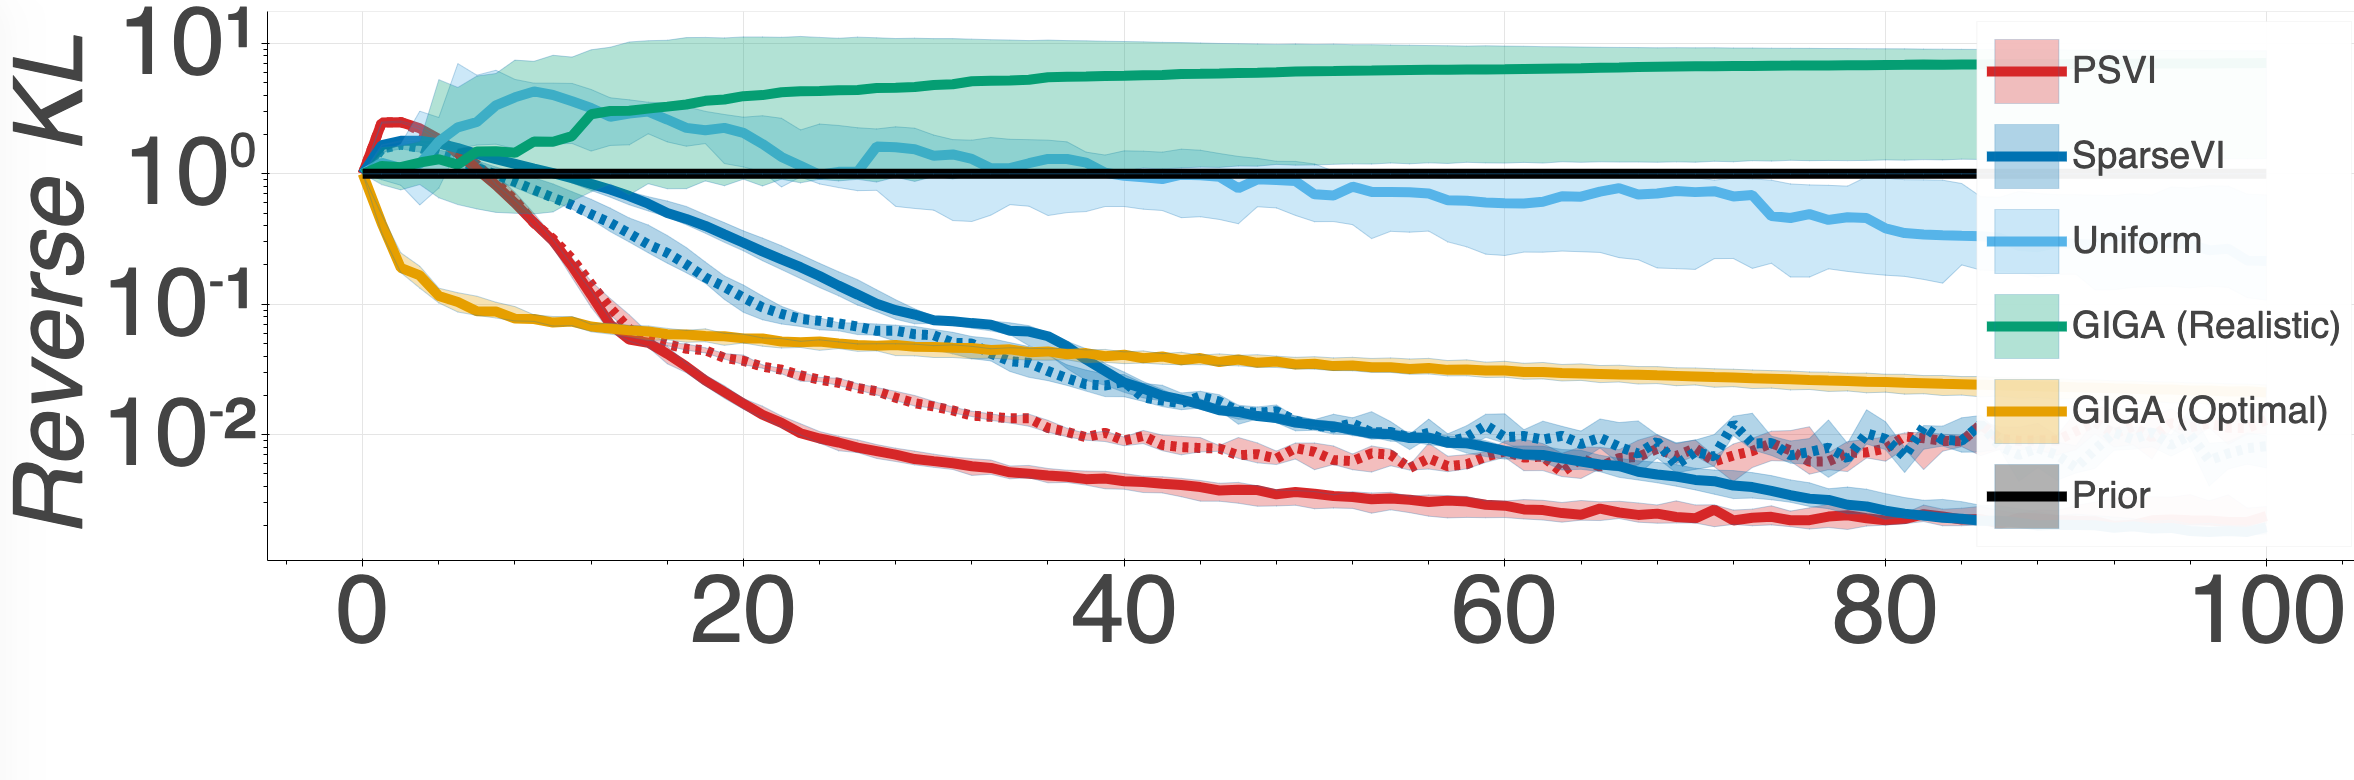
\includegraphics[width=0.475\textwidth]{\MyPath/tempfigs/synthlriter.png} \hfill 
		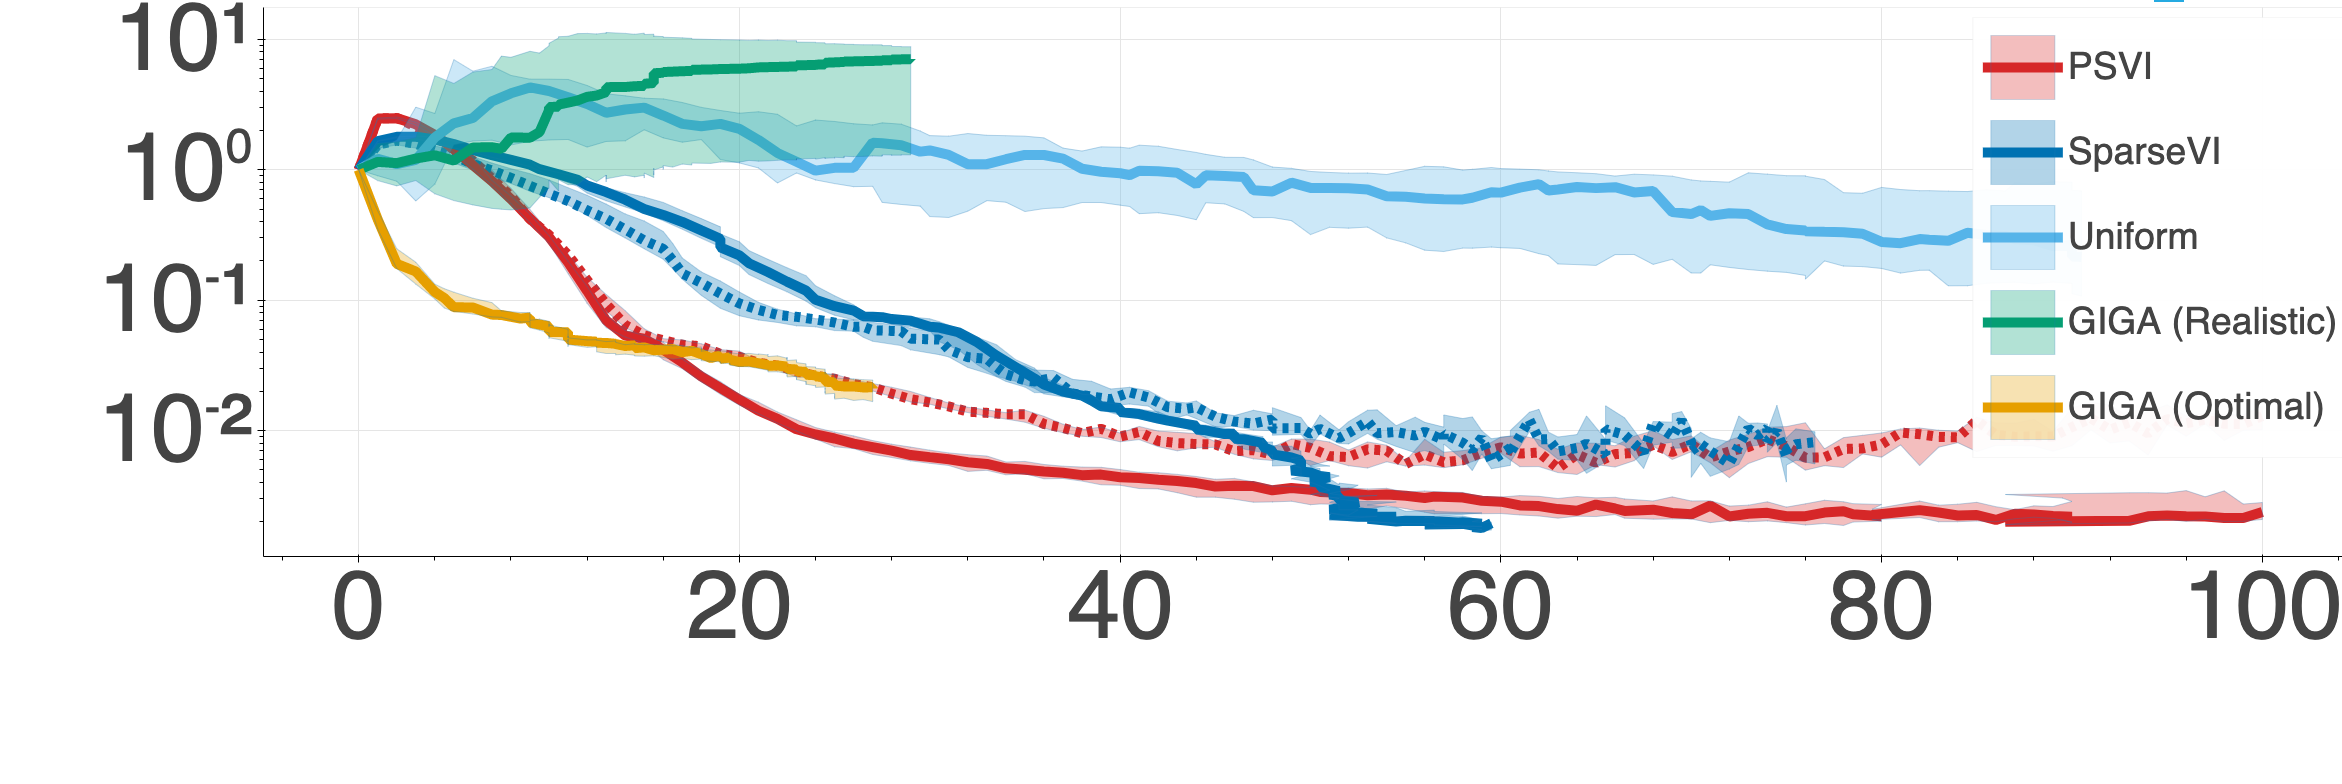
\includegraphics[width=0.475\textwidth]{\MyPath/tempfigs/synthlrsz.png}%
	\end{subfigure}\hfill\qquad
	\begin{subfigure}[b]{\textwidth}
		\centering
		\caption*{\textsc{Phishing}}
		\vspace*{-0.3cm}
		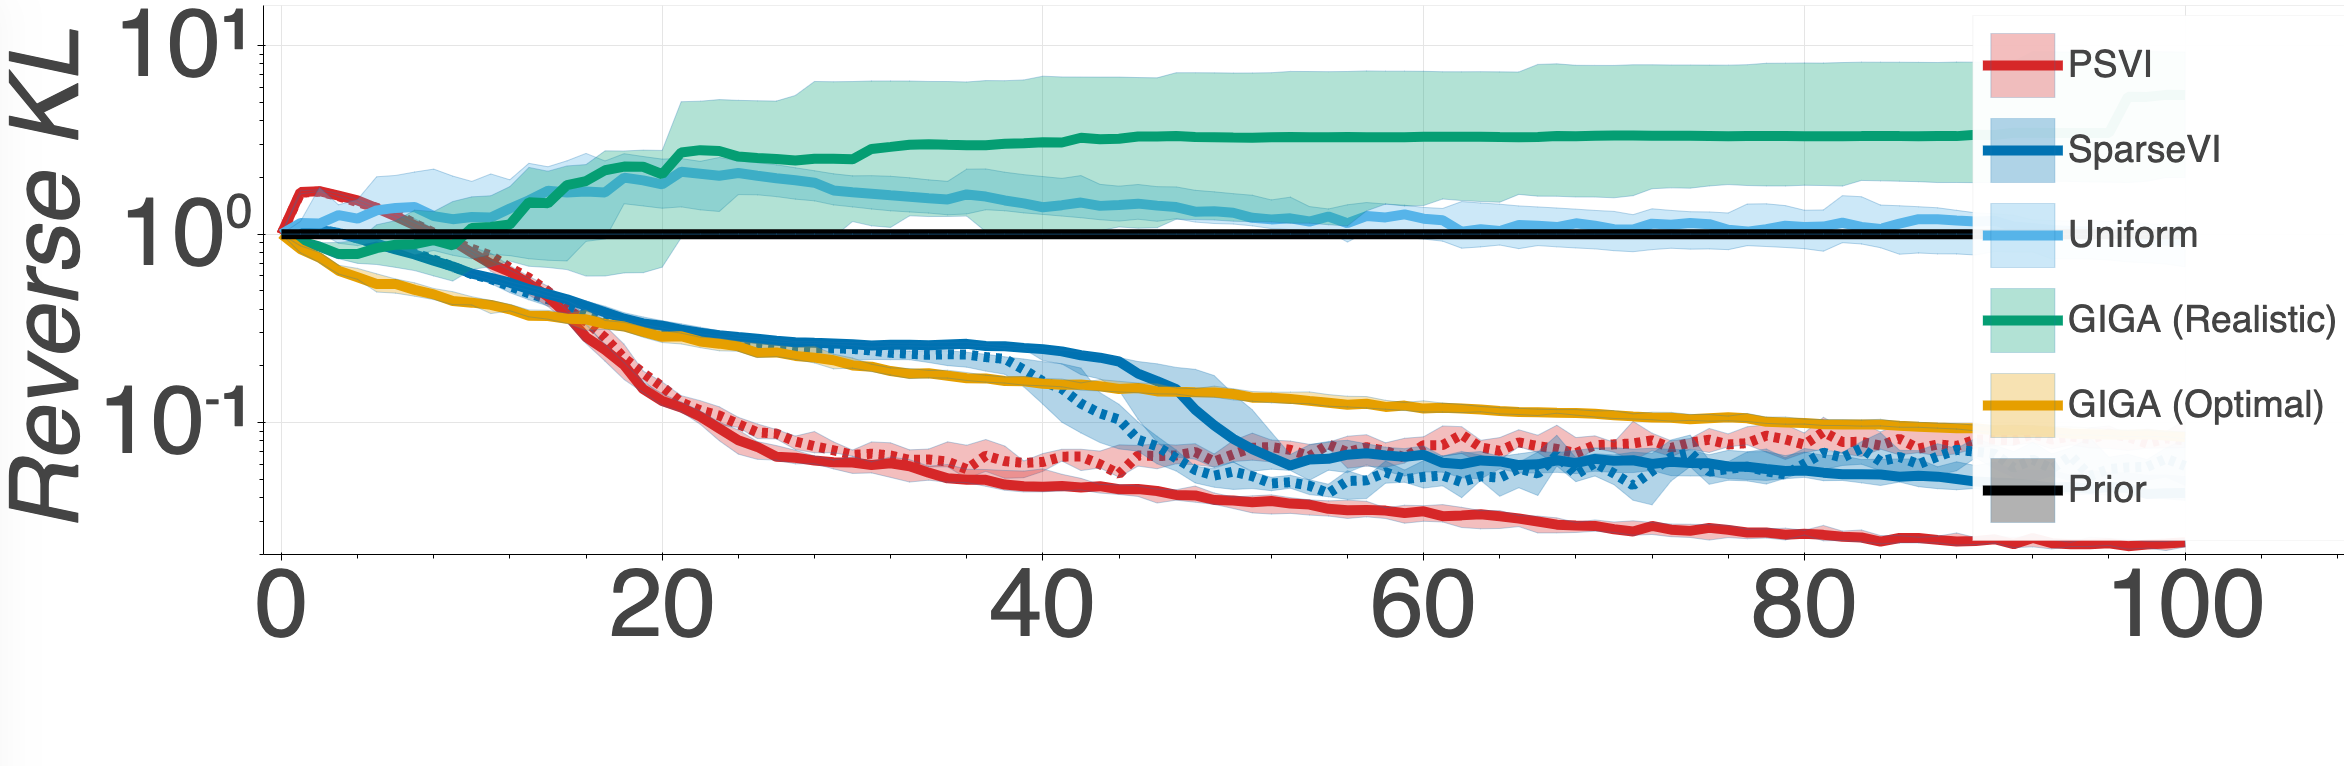
\includegraphics[width=0.475\textwidth]{\MyPath/tempfigs/phishingiter.png} \hfill
		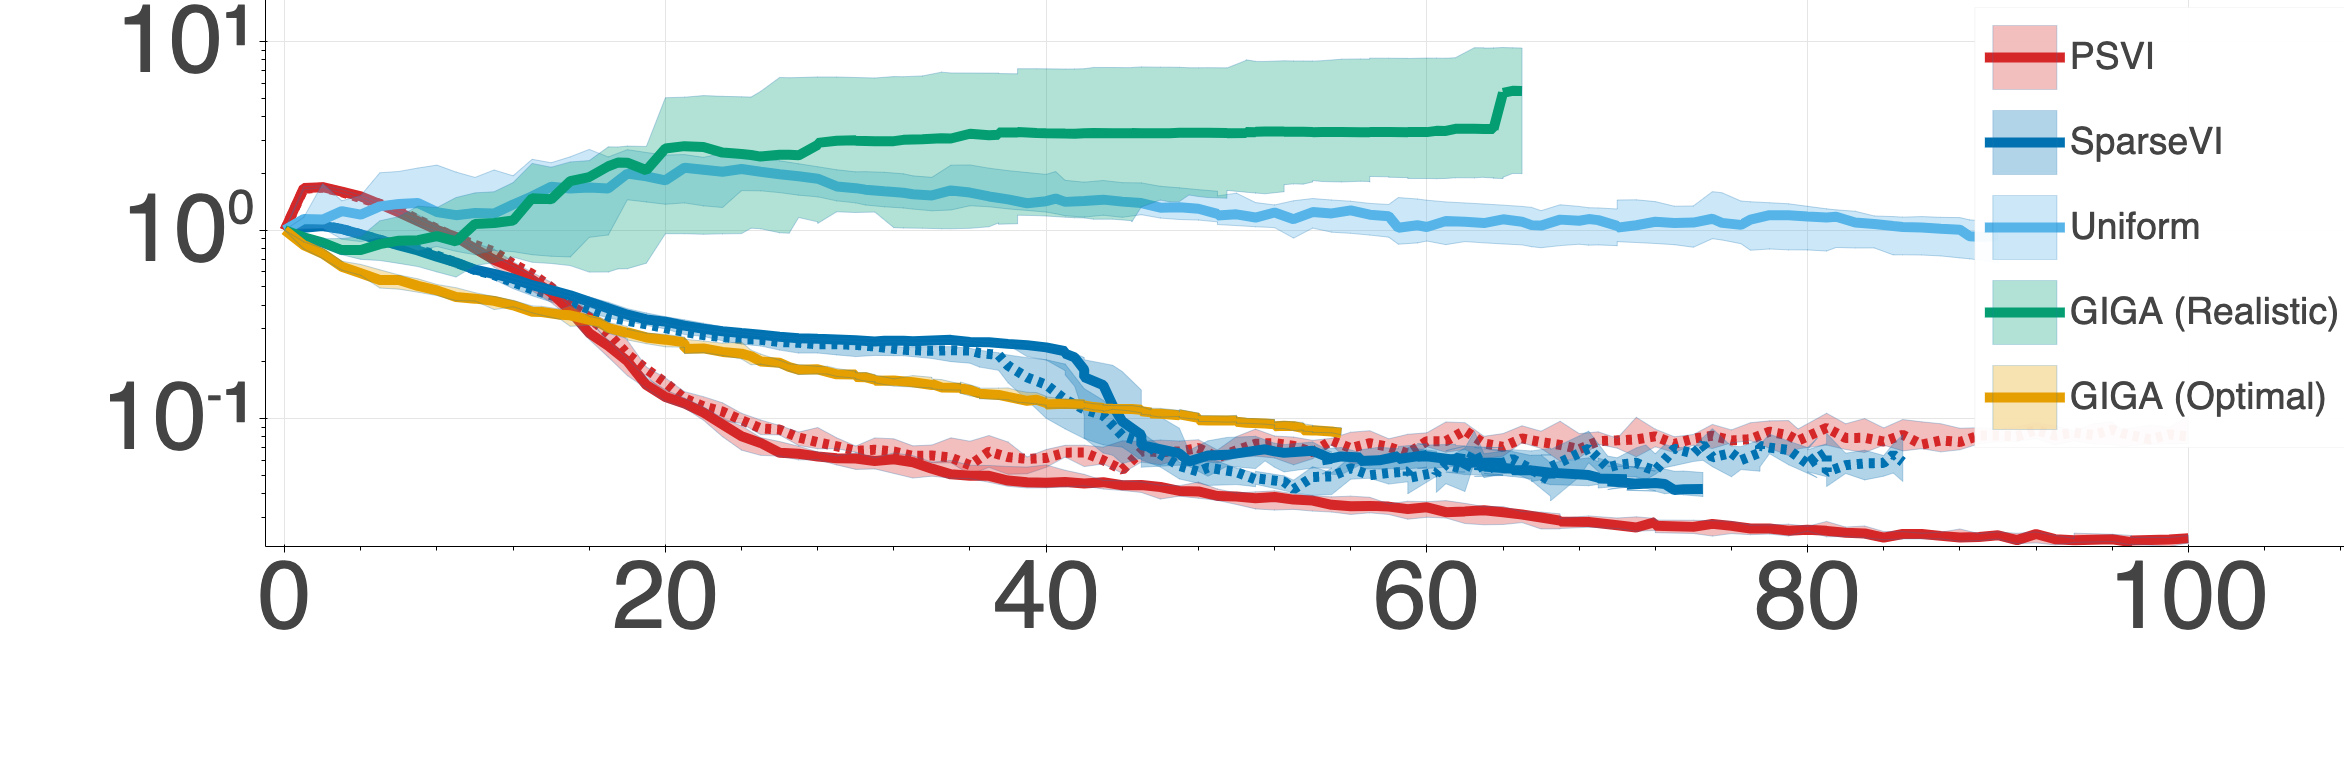
\includegraphics[width=0.475\textwidth]{\MyPath/tempfigs/phishingsz.png}%
	\end{subfigure}\hfill\qquad
	\begin{subfigure}[b]{\textwidth}
				\centering
		\caption*{\textsc{ChemReact}}
		\vspace*{-0.3cm}
		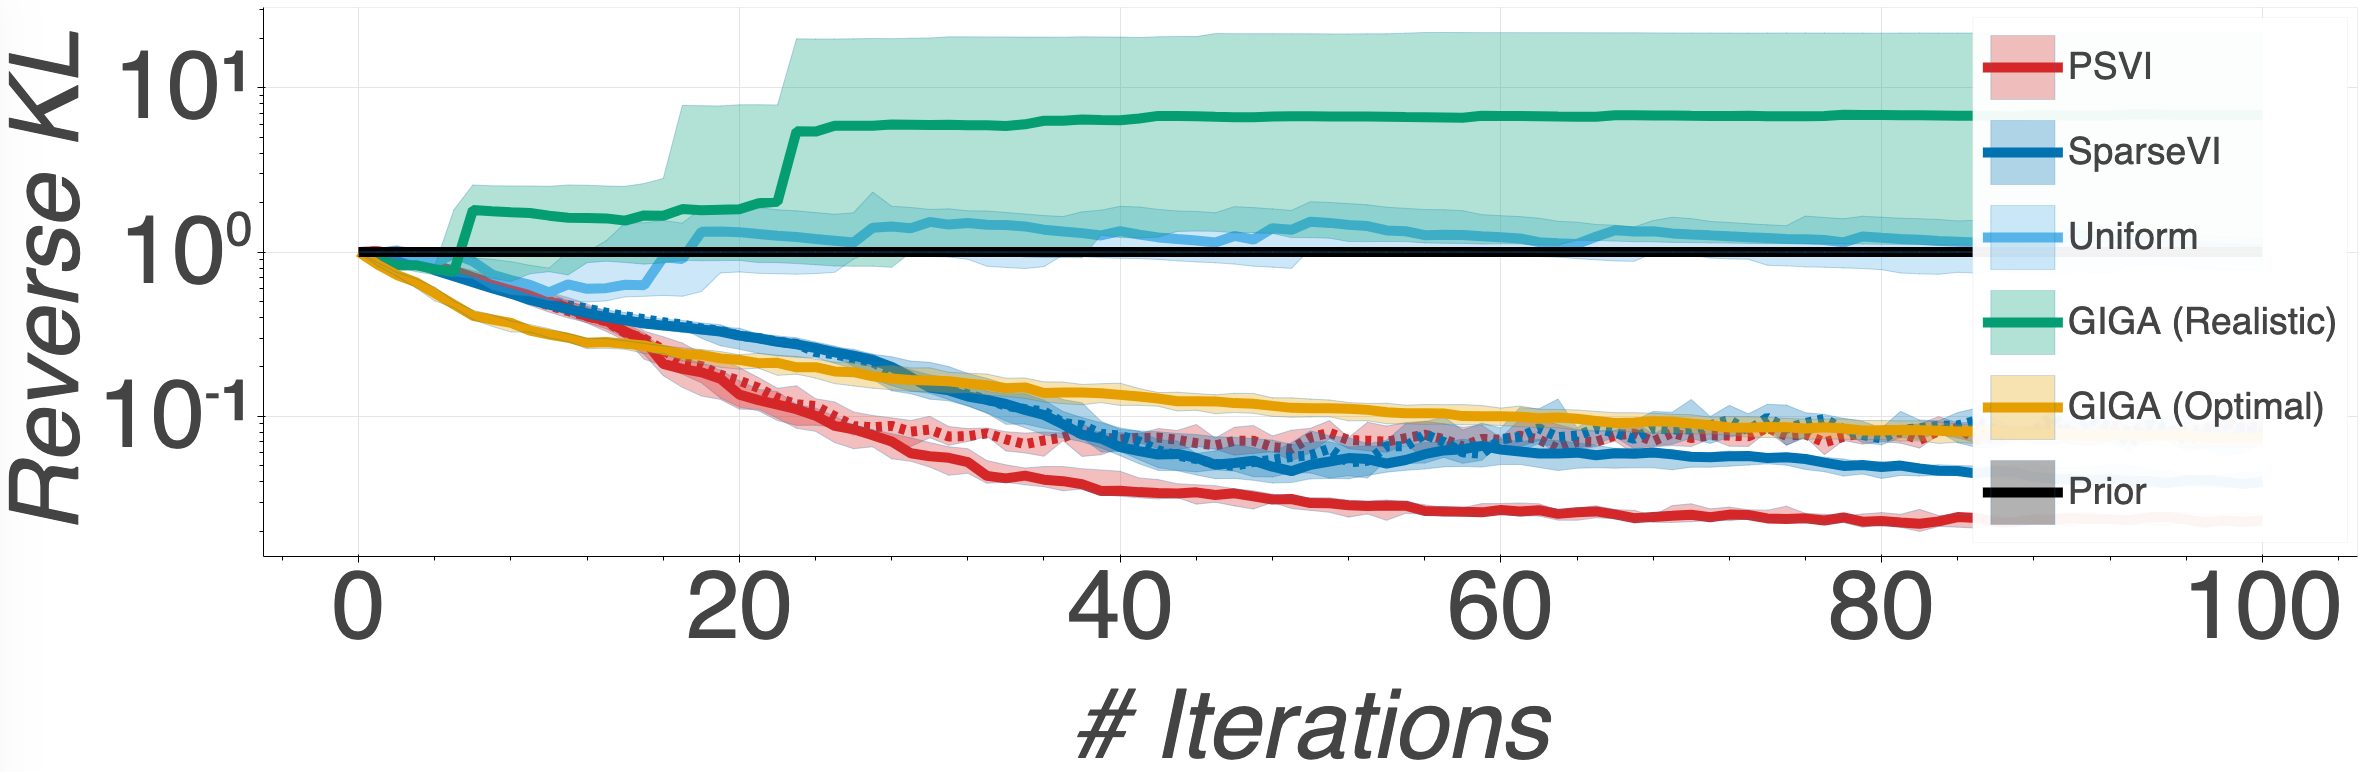
\includegraphics[width=0.475\textwidth]{\MyPath/tempfigs/ds1iter.png}
		\hfill
		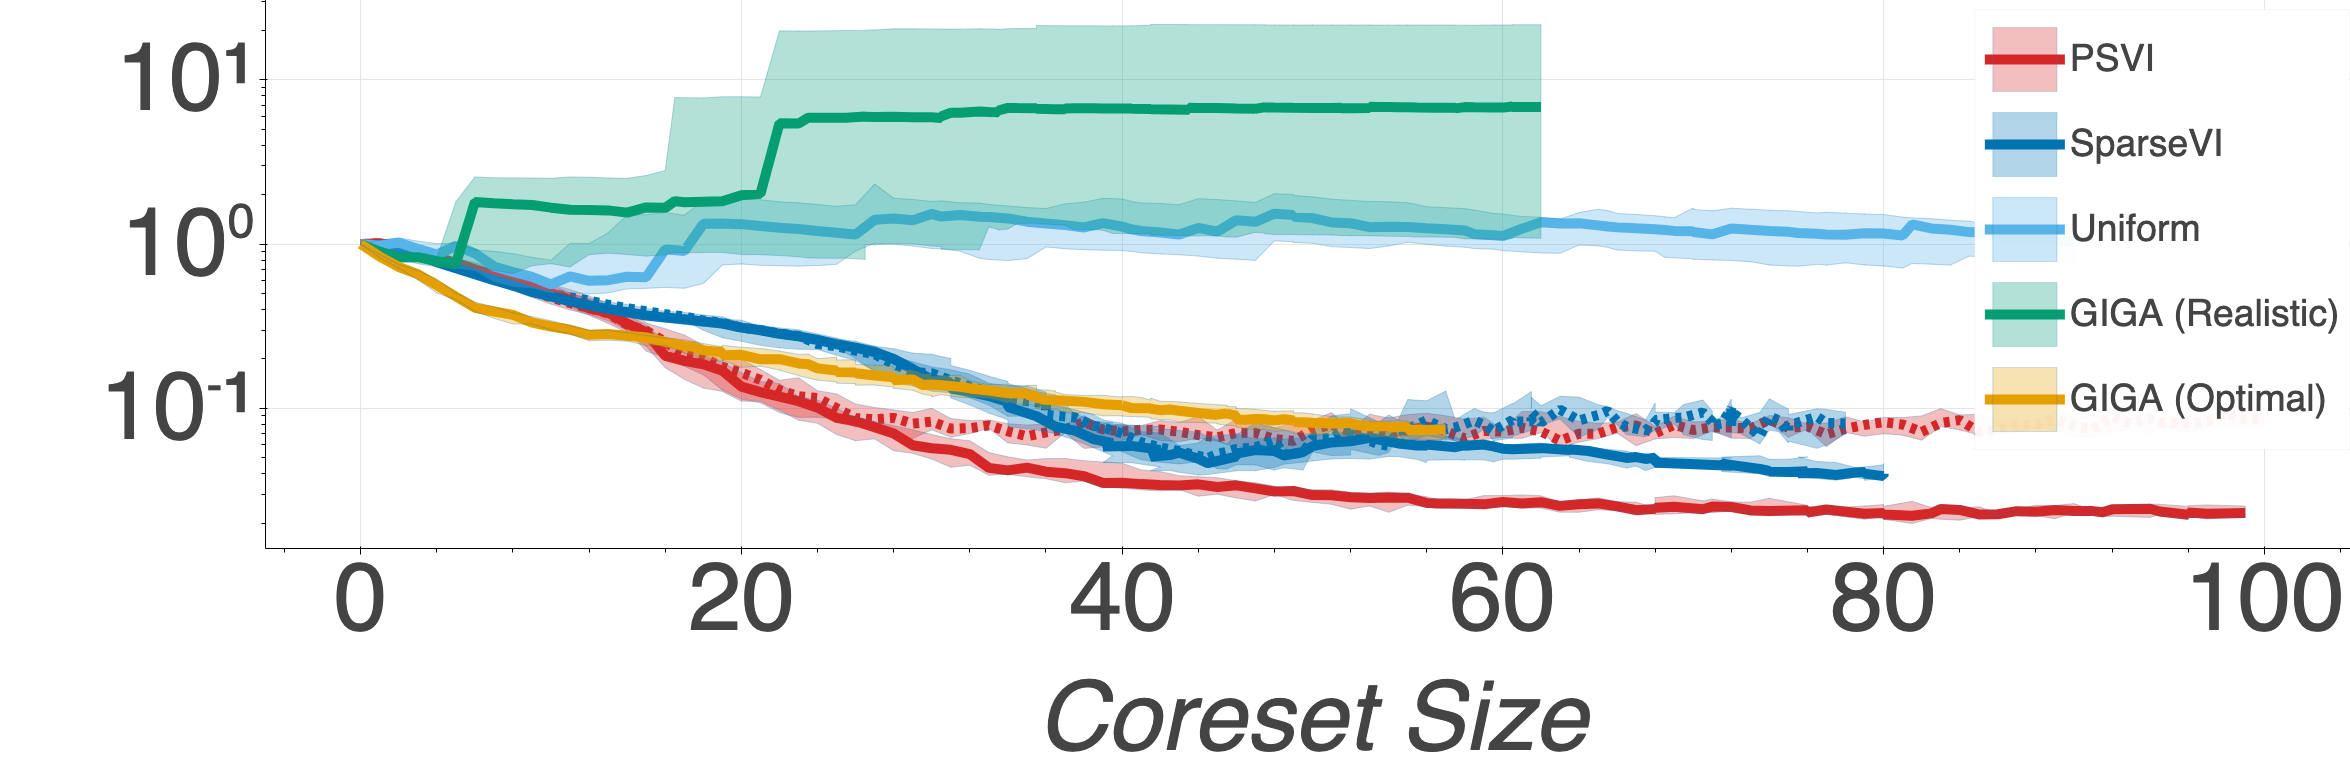
\includegraphics[width=0.475\textwidth]{\MyPath/tempfigs/ds1sz.png}%
	\end{subfigure}
	\caption{Comparison of incremental \psvi~and \sparsevi~approximate posterior
		quality vs iterations of incremental construction~(\emph{left}) and  coreset
		size~(\emph{right}) for logistic regression on small-scale experiment. With dashed lines is displayed the posterior quality achieved
		by incremental \psvi~and \sparsevi~constructions using gradients computed on data subsets of size $256$.}
	\label{fig:logreg_dkl}
\end{figure*}



\paragraph{Evaluation of CPU time requirements} Experiments were performed on a CPU cluster node with a 2x Intel Xeon Gold 6142 and 12GB RAM. In the case of \psvi~the computation of coreset sizes from 1 to 100 was parallelized per single size over 32 cores in total. \cref{fig:30logreg_dkl_cput} shows posterior approximation error vs required CPU time for all coreset construction algorithms over logistic regression on the small-scale and large-scale datasets. As opposed to existing incremental coreset construction schemes, batch construction of \psvi~reduces the dependence between coreset size and processing cost: for \sparsevi~$\Theta(M^2)$ gradient computations are required, as this method builds up a coreset one point at a time; in contrast, \psvi~requires $\Theta(M)$ gradients since it learns all pseudodata points jointly. Although each gradient step of \psvi~is more expensive, practically this implies a steeper decrease in approximation error over processing time compared to \sparsevi. In the case of differentially private \psvi,~some extra CPU requirements are added due to the subsampled Gaussian mechanism computations.


\paragraph{Incremental scheme for pseudocoreset construction} We also experimented with an \emph{incremental scheme for pseudocoreset} construction. According to this scheme, pseudodata points are added sequentially to the pseudocoreset. Similarly to \sparsevi, in the beginning of each coreset iteration, we initialize a new pseudodata point at the true datapoint which maximizes correlation with current residual approximation error. Next, we jointly optimize the most recently added pseudodata point location, along with the pseudocoreset weights vector, over a gradient descent loop.  As opposed to batch construction, for large coreset sizes the incremental scheme for \psvi~does not achieve savings in CPU time compared to \sparsevi.

We evaluated coreset construction methods on Bayesian logistic regression. We used $M=100$ iterations for construction, $ S=100 $ Monte Carlo samples per gradient estimation, $ T= 100$ iterations for optimization, and learning rate $\gamma_t \propto 0.5t^{-1}$. Coreset posterior samples over the course of construction
for \sparsevi~and incremental \psvi~were drawn from a Laplace approximation using current
coreset weights and points. We implemented~\sparsevi~and incremental~\psvi~via computing gradients on the full dataset, as well as using stochastic gradients on subsets of size $B=256$ for lowering computational cost. 

 Results presented in~\cref{fig:logreg_dkl} demonstrate that incremental \psvi~achieves consistently the smallest posterior approximation error, offering improvement
compared to \sparsevi~and even achieving better performance than \gigao. %, without the requirement for specifying a weighting function.  
 We observe that stochastic gradients implementation~(dashed lines) reaches a plateau at higher values of KL compared to full gradients~(solid lines), but still achieves performance comparable with~\gigao.








\chapter{$\beta$-Cores: Robust Large-Scale Bayesian Data Summarization in the Presence of Outliers}
\label{chap:chap5}
\renewcommand*{\MyPath}{../Chapter5}%
{
	Modern machine learning applications should be able to address the intrinsic challenges arising over inference on massive real-world datasets, including scalability and robustness to outliers. Despite the multiple benefits of Bayesian methods (such as uncertainty-aware predictions, incorporation of experts knowledge, and hierarchical modeling), the quality of classic Bayesian inference depends critically on whether observations conform with the assumed data generating model, which is impossible to guarantee in practice. In this chapter, we propose a variational inference method that, in a principled way, can simultaneously scale to large datasets, and robustify the inferred posterior with respect to the existence of outliers in the observed data. Reformulating Bayes theorem via the \bdiv, we posit a robustified pseudo-Bayesian posterior as the target of inference. Moreover, relying on the recent formulations of Riemannian coresets for scalable Bayesian inference, we propose a sparse variational approximation of the robustified posterior and an efficient stochastic black-box algorithm to construct it. Overall our method allows releasing cleansed data summaries  that can be applied broadly in scenarios including structured data corruption. We illustrate the applicability of our approach in diverse simulated and real datasets, and various statistical models, including Gaussian mean inference, logistic and neural linear regression, demonstrating its superiority to existing Bayesian summarization methods in the presence of outliers. %Furthermore, our dataset reduction scheme enables us to efficiently compute data Shapley value approximations, making a decisive step towards equitable valuation of individual information in massive scale data marketplaces.
}

This chapter is based on~\citep{beta-cores}.
\section{Introduction}
\label{sec:introduction}

Machine learning systems perpetually collect growing datasets, such as product reviews, posting activity on social media, users feedback on services, or insurance claims. The rich information content of such datasets has opened up an exciting potential to remedy various practical problems. Hence, recent years have witnessed a surge of interest in scaling up inference in the large-data regime via stochastic and batch methods~\cite{angelino16, hoffman13, welling11}. Most of related approaches have treated datapoints indiscriminantly; nevertheless, it is well known that not all datapoints contribute equally valuable information for a given target task~\cite{ghorbani19}. 

Datasets collected in modern applications contain redundant input samples that reflect very similar statistical patterns, or multiple copies of identical observations. Often input aggregates subpopulations emanating from different distributions~\cite{zheng08, zhuang15}. Moreover, the presence of outliers is a ubiquitous challenge, attributed to multiple causes. In the first place, noise is inherent in most real-world data collection procedures, creating systematic outliers: crowdsourcing is prone to mislabeling~\cite{frenay13} and necessitates laborious data cleansing~\cite{lewis04, paschou10}, while measurements commonly capture sensing errors and system failures. Secondly, outliers can be generated intentionally from information contributing parties, who aim to compromise the functionality of the application through data poisoning attacks~\cite{barreno10, biggio12, li16, koh17, steinhardt17, ghorbani19}, realised for example via data generation from fake accounts. Outliers detection is  challenging, particularly in high dimensions~\cite{lucic16outliers, diakonikolas19, dickens20}. Proposed solutions \mbox{often are} model-specific, and include dedicated learning components which increase the time complexity of the application, involve extensive hyperparameter tuning, introduce data redundancies, or require model retraining~\cite{sheng08, whitehill09, raykar10, karger11, liu12, zhang16}. On the other hand, operating on a corrupted dataset is brittle, and can decisively degrade the predictive performance of downstream statistical tasks, deceptively underestimate model uncertainty and lead to incorrect decisions. 

In this work, we design an integrated approach for inference on massive scale observations that can jointly address scalability and data cleansing for complex Bayesian models, via robust data summarization. Our method inherits the full set of benefits of Bayesian inference and works for any model with tractable likelihood function. At the same time, it maintains a high degree of automation with no need for manual data inspection, no additional computational overhead due to robustification, and can tolerate a non-constant number of corruptions. Moreover, our work points to a more efficient practice in large-scale data acquisition, filtering away less valuable samples, and indicating the regions of the data space that are most beneficial for our inference task. 

Our solution can be regarded as an extension of Bayesian coreset methods that can encompass robustified inference. Bayesian coresets~\cite{huggins16, campbell19jmlr, campbell19neurips} have been recently proposed as a method that enables Bayesian learning at scale via substituting the complete dataset over inference with an informative sparse subset thereof. Robustified Bayesian inference methods~\cite{berger94} have sought solutions to mismatches between available observations and the assumed data generating model, %via generalizing the data likelihood function, 
via proposing heavy-tailed data likelihood functions~\cite{huber09, insua12} and localization~\cite{definetti61, wang18}, using robust statistical divergences~\cite{futami18, knoblauch18, miller19},  or inferring datapoints-specific importance weights~\cite{wang17}. Here, we cast coreset construction in the framework of robustified inference, introducing \emph{\bcores{}}, a method that learns sparse variational approximations of the full data posterior under the \bdiv{}. In this way, we are able to yield summaries of large data that are distilled from outliers, or data subpopulations departing from our statistical model assumptions. Importantly, \bcores{} can act as a preprocessing step, and the learned data summaries can subsequently be given as input to any ordinary or robustified black-box inference algorithm.

The rest of this chapter is organized as follows. In \cref{sec:preliminaries,sec:method} we introduce necessary concepts from Bayesian inference, and present our proposed method. In \cref{sec:evaluation} we expose experimental results on simulated and real-world benchmark datasets: we consider diverse statistical models and scenarios of extensive data contamination, and demonstrate that, in contrast to existing summarization algorithms, our method is able to maintain reliable predictive performance in the presence of structured and unstructured outliers. Finally, in \cref{sec:conclusion} we provide conclusions and discuss future works.

This chapter is based on~\citep{beta-cores}.





\section{Preliminaries}
\label{sec:preliminaries}

In this section, we introduce the required concepts from Bayesian inference, present robustness limitations of standard posterior on big data, and outline existing generalizations of the posterior that aim to robustify inference with respect to data mismatch.

\subsection{Standard Bayesian inference and lack of robustness in the large-data regime}
In the context of Bayesian inference, we are interested in updating our beliefs about a vector of random variables $\theta \in \Theta$, initially expressed through a prior distribution $\pi_0(\theta)$, after observing a set of datapoints $ x:=(x_n)_{n=1}^{N} \in \mcX^N$.  Posterior on $\theta$ can be computed via the application of Bayes rule 
\[
\pi(\theta|x) = \frac{1}{Z'}\pi(x|\theta)\pi_0(\theta),
\label{eq:bayes-rule}
\] 
where $Z'$ is a (typically intractable) normalization constant, and $\pi(x|\theta)$ is the likelihood of our observations according to an assumed statistical model.
When datapoints are conditionally independent given $\theta$---which is the primary focus of this work---likelihood gets factorized as $\pi(x|\theta) = \Pi_{n=1}^{N}\pi(x_n|\theta)$. An equivalent formulation of  the
Bayesian posterior as a solution to an optimization problem was proposed by Zellner~\citep{zellner88}, which is written as  
\[
\pi(\theta|x) = \frac{1}{Z'} \exp\left(-\xent{\hpi(x)}{\pi(x|\theta)}\right)\pi_0(\theta).
\label{eq:zellner-rule}
\]
In the above, $\hpi(x)$ is the empirical distribution of the observed datapoints. The exponent $\xent{\hpi(x)}{\pi(x|\theta)}:=-\sum_{n=1}^{N}\log\pi(x_n|\theta)$
corresponds (up to a constant) to the \emph{cross-entropy}, which is  equal to the empirical average of negative log-likelihoods of the datapoints, and quantifies the expected loss incurred by our estimates for the model parameters $\theta$ over the available observations, under the \emph{Kullback-Leibler~(KL) divergence}.

When $N$ is large, the Bayesian posterior is strongly affected by perturbations in the observed data space. To develop an intuition on this, assuming that the true and observed data distributions have densities $\pi_\theta$ and $\pi_\textsubscript{obs}$ respectively, we can rewrite an approximation of~\cref{eq:zellner-rule} via the KL divergence ($\plainkl$) as~\cite{miller19}
\[
\pi(\theta|x) 
& \propto  \exp\left(\sum_{n=1}^{N}\log\pi(x_n|\theta)\right) \pi_0(\theta)
\doteq	 \exp\left(N \int \pi_\textsubscript{obs} \log \pi_\theta\right) \pi_0(\theta) \\
 &:= \exp\left(-N \kl{\pi_\textsubscript{obs}}{\pi_\theta}\right) \pi_0(\theta),
 \label{eq:missmatch_with_N}
\]
where $\doteq$ denotes  agreement to first order in exponent.\footnote{i.e. $a_n \doteq b_n$ iff $(1/n)\log(a_n/b_n) \rightarrow 0$}
Hence, due to the large $N$ in the exponent, small changes to $\pi_\textsubscript{obs}$ will have a large impact on the posterior.

\subsection{Robustified posteriors}

Robust inference methods aim to adapt~\cref{eq:bayes-rule} to formulations that can address the case of observations departing from model assumptions, as often happening in practice, e.g. due to misspecified shapes of data distributions and number of components, or due to the presence of outliers. In such formulations~\citep{dawid16, jewson18, fujisawa08, eguchi01}, Bayesian updates rely on utilising robust divergences instead of the KL divergence, to express the losses over the data. 

A popular choice~\citep{futami18, knoblauch18} for enhancing robustness of inference is replacing the log-likelihood terms arising in~\cref{eq:zellner-rule} with the \emph{\bdiv~}(or \emph{density power divergence})~\citep{basu98, cichocki10}, which yields the following posterior for $\theta$~\citep{ghosh16,knoblauch18}
\[
\pi_\beta(\theta|x) \propto \exp\left(-\db{\hpi(x)}{\pi(x|\theta)}\right)\pi_0(\theta),
\label{eq:b-posterior}
\] 
where 
\[
\db{\hpi(x)}{\pi(x|\theta)} := 
 -\sum_{n=1}^{N}  \underbrace{\left(\frac{\beta+1}{\beta}\pi(x_n|\theta)^{\beta} + \int_{\mcX} \pi(\chi|\theta)^{1+\beta}d\chi\right)}_{:=f_n(\theta)},
\label{eq:b-loss}
\]
with $\beta>0$.
We refer to quantities defined in~\cref{eq:b-posterior,eq:b-loss} as the \emph{\bpost{}} and \emph{\blik{}} respectively. Noticeably, the individual terms $f_n(\theta)$  of the \blik{} %, which are known as the Tsallis scores~\citep{tsallis88}, are decomposed into a data-independent $c(\theta)$, and a data-dependent part $t_n(\theta)$.
% := \frac{1}{\beta} \pi(x_n|\theta)^{\beta}$. 
%The latter 
allow attributing \emph{different strength of influence to each of the datapoints}, depending on their accordance with the model assumptions. As densities get raised to a suitable power $\beta$, outlying observations are exponentially downweighted. When $\beta \rightarrow 0$,~\cref{eq:zellner-rule} is recovered and all datapoints are treated equally.

In the presentation above we focused on modeling observations $(x_n)_{n=1}^{N}$~(unsupervised learning). In the case of supervised learning on data pairs ${(x_n,y_n)}_{n=1}^{N} \in (\mcX \times \mcY)^N$, the respective expression for individual terms of \blik{}\footnote{In this context for simplicity we use notation $f_n(\cdot)$  to denote $f(y_n|x_n, \cdot)$.} is~\cite{basu98}
\[
f_n(\theta):= -\frac{\beta+1}{\beta}\pi(y_n|x_n,\theta)^{\beta} +  \int_{\mcY} \pi(\psi|x_n,\theta)^{1+\beta}d\psi.
\label{eq:sl-lik-terms}
\] 
\section{Method}
\label{sec:method}

In this section we discuss \bcores, our unified solution to the robustness and scalability challenges of large-scale Bayesian inference. \cref{subsec:sparse-b-posterior} introduces the main quantity of interest in our inference method, and shows how it addresses the exposed issues. \cref{subsec:bb-construct} presents an iterative algorithm that allows efficient approximate computations of our posterior.


\subsection{Sparse \bpost{}}
\label{subsec:sparse-b-posterior}


Scaling up the computation of the robust $\beta$-posterior~\cref{eq:b-posterior} in the regime of massive datasets for non-conjugate models is challenging:
%~Closed form computation of~\bdiv{} is not possible for a large number of statistical models. Moreover, 
similarly to the standard Bayesian posterior~\cref{eq:bayes-rule}, applying Markov chain Monte Carlo~(MCMC) methods to sample from the~\bpost{}, implies a computational cost scaling at order $\Theta(N)$. 

Bayesian coresets~\cite{huggins16,campbell19jmlr} have been recently proposed as a method to circumvent the computational cost for the purposes of approximate inference via summarizing the original dataset  $(x_n)_{n=1}^{N}$ with a small learnable subset of weighted datapoints $(x_m, w_m)_{m=1}^{M}$, where  $(w_m)_{m=1}^{M} \in \reals^{M}_{+},\; M \ll N$. 
Substituting~\cref{eq:b-loss} in ~\cref{eq:b-posterior}, allows us to explicitly introduce a weights vector $ w \in \reals_{\geq 0}^{N}$ in the posterior, and rewrite the latter in the general form
\[
\pi_{\beta,w}(\theta|x) 
= \frac{1}{Z(\beta, w)}  \exp\left(\sum_{n=1}^{N}w_nf_n(\theta)\right)\pi_0(\theta).
\label{eq:bcore-posterior}
\]
%In the last line the data-independent part of the Tsallis score has been absorbed in the uknown log-partition function of the distribution.
In the case of the \bpost{} on the full dataset~\cref{eq:b-posterior}, we have $w=\vecone \in\reals^{N}$; for coreset posteriors this vector acts as a learnable parameter and attains a non-trivial sparse value, with non-zero entries corresponding to the elements of the full dataset that are selected over the summarization.

Although Bayesian coresets can dramatically reduce inference time, they inherit the susceptibility of Bayesian posterior to data mismatch in the large data regime: even though the number of points used in inference gets reduced, these points are now weighted, hence the remark of~\cref{eq:missmatch_with_N} can carry over in coresets posterior. 

The recent formulation of Riemannian coresets~\citep{campbell19neurips} has framed the problem of coreset construction as Variational Inference~(VI) in a sparse exponential family. Our method provides a natural extension of this framework to robust divergences. Here we aim to approximate data posterior via a \emph{sparse \bpost}, which can be expressed as follows
\[
w^{*} = \arg \min_{w\in\reals^{N}} \kl{\pi_{\beta,w}}{\pi_{\beta}} 
\quad
\text{s.t.}
\quad
w \geq 0,\; ||w||_0 \leq M,
\label{eq:coreset-vi}
\]
%where $\plainkl$ is the KL divergence. 
In the following we denote expectations and covariances under $\theta \sim \pi_{\beta,w}(\theta|x)$ as $\EE_{\beta,w}$ and $\cov_{\beta,w}$ respectively. Then the KL divergence is written as
\[
\kl{\pi_{\beta,w}}{\pi_{\beta}}:=\EE_{\beta, w} \left[\log\frac{\pi_{\beta,w}}{\pi_\beta}\right].
\label{eq:kld}
\]
In our formulation it is easy to observe that posteriors of~\cref{eq:bcore-posterior} form a set of \emph{exponential family distributions}~\cite{wainwright08}, with natural parameters $w \in \reals_{\geq 0}^N$, sufficient statistics $(f_n(\theta))_{n=1}^{N}$, and log-partition function $\log Z(\beta, w)$. Following~\citep{campbell19neurips}, the objective can be expanded as 
\[
\kl{\pi_{\beta,w}}{\pi_{\beta}} =& \log Z(\beta) - \log Z(\beta, w) 
                                    - \sum_{n=1}^{N}\EE_{\beta,w}\left[f_n(\theta)- w_n f_n(\theta)\right],
\label{eq:sparsevi-obj}
\]
and minimized via gradient descent on %$\beta$ and 
$w$.  %As detailed in~\cref{sec:gradient-derivations}, 
The gradient of the objective of~\cref{eq:sparsevi-obj} can be derived in closed form, as  
\[
\nabla_{w}\kl{\pi_{\beta,w}}{\pi} 
												   & = -\cov_{\beta,w}\left[f,(1 -w)^Tf\right], 
\label{eq:dkl-grad}
\]
where $f:=\left[f_1(\theta) \ldots f_N(\theta)\right]^T$.%, $f':=\left[f'_1(\theta) \ldots f'_N(\theta)\right]^T$.




\subsection{Black-box stochastic scheme for incremental coreset construction}
\label{subsec:bb-construct}



\begin{algorithm*}[!t]
	\caption{Incremental construction of sparse \bpost{}}
	\label{alg:bcores}
	\begin{algorithmic}[1]
		\Procedure{\bcore}{$f,  \pi_0, x, M, B, S, T, (\gamma_t)_{t=1}^{\infty}$, $\beta$}
		\State $w \assign \mathbf{0} \in \reals^{M}$,\;\; $g \assign \mathbf{0} \in \reals^{S \times M}$, \;\;$g' \assign \mathbf{0} \in \reals^{S \times B}$, \;\;$\mcI \assign \emptyset$
		\For{$m =1, \ldots, M $}
		\LineCommentIndent{Take S samples from current coreset posterior}
		\State $(\theta)_{s=1}^{S}  \distiid \pi_{\beta,w} \propto \exp \left(w^Tf\right) \pi_0(\theta)$
		\LineComment{Obtain a minibatch of $B$ datapoints from the full dataset}
		\State $\mcB\dist\distUnifSubset\left([N], B\right)$
		\LineComment{Compute the \blik{} vectors over the coreset and minibatch datapoints for each sample}
		\State $g_{s} \gets \left( f(x_m, \theta_s, \beta ) - \frac{1}{S}\sum_{r=1}^S f(x_m, \theta_{r}, \beta) \right)_{m \in \mcI}\in \reals^M$ 
		\State  $g'_{s} \gets \left( f(x_b, \theta_s, \beta) - \frac{1}{S}\sum_{r=1}^S f(x_b, \theta_{r}, \beta) \right)_{b\in\mcB} \in \reals^B$
		\LineComment{Get empirical estimates of correlation over the coreset and minibatch datapoints}
		\State $\hcorr \assign \diag \left[ \frac{1}{S} \sum_{s=1}^{S} g_{s}
		{g_{s}}^T\right]^{-\frac{1}{2}} \left(\frac{1}{S} \sum_{s=1}^{S} g_{s} \left(\frac{N}{B}1^T g'_{s} - w^T g_{s}\right)\right) \in \reals^{M}$
		\label{lst:line:core-corr}
		\State $\hcorr' \assign \diag \left[ \frac{1}{S} \sum_{s=1}^{S} g'_{s}
		{g'_{s}}^T\right]^{-\frac{1}{2}} \left(\frac{1}{S} \sum_{s=1}^{S} g'_{s} \left(\frac{N}{B}1^T g'_{s} - w^T g_{s}\right)\right)  \in \reals^{B}$
		\label{lst:line:batch-corr}
		\LineComment{Add next datapoint via correlation maximization}
		\State $n^{\star} \assign \arg \underset{n \in [m] \cup [B]}{\max} \left( \left|\hcorr \right| \cdot \vecone[n \in \mcI] + \hcorr' \cdot \vecone [n \notin \mcI]\right)$, \;\;$ \mcI \assign \mcI \cup \{n^{\star}\}$
		\For{$ t = 1, \ldots, T$} 		\Commenttriangle{Optimize weights vector via projected gradient descent}
		\State $(\theta)_{s=1}^{S}  \distiid \pi_{\beta,w}(\theta) \propto \exp\left(w^T f\right)\pi_0(\theta)$ 
		\State $\mcB\dist\distUnifSubset\left([N], B\right)$
		\LineComment{Compute gradient terms discretizations over the coreset and minibatch datapoints for each sample}
		\For{$s = 1, \dots, S$} 
		\State $g_{s} \gets \left( f(x_m, \theta_s, \beta) - \frac{1}{S}\sum_{r=1}^S f(x_m, \theta_{r}, \beta) \right)_{m\in\mcI} \in \reals^M$  
		\State $g'_{s} \gets \left( f(x_b, \theta_s, \beta) - \frac{1}{S}\sum_{r=1}^S f(x_b, \theta_{r}, \beta) \right)_{b\in\mcB} \in \reals^B$  	
		\EndFor
		\LineComment{Compute MC gradients for variational parameters}
		\State $\hat\nabla_w \gets -\frac{1}{S}\sum_{s=1}^S g_s\left( \frac{N}{B} 1^Tg'_s- w^Tg_s\right)$
		%, $\hat\nabla_\beta \gets -w^T\frac{1}{S}\sum_{s=1}^S k_s\left( \frac{N}{B} 1^Tg'_s- w^Tg_s\right)$
		\label{lst:line:mc-grad}
		\LineComment{Take a projected stochastic gradient step}
		\State $w \gets \max(w - \gamma_t\hat\nabla_w, 0)$
		%, $\beta \gets \max(\beta - \gamma_t\hat\nabla_\beta, 0)$
		\EndFor
		\EndFor
		\State\Return $w$%, $\beta$
		\EndProcedure		 
	\end{algorithmic}
\end{algorithm*}


To scale up coreset construction on massive datasets we use stochastic gradient descent on minibatches $\mcB \sim \distUnifSubset([N], B)$, with $B \ll N$.
The covariance of~\cref{eq:dkl-grad} required for exact gradient computation of the variational objective is generally not available in analytical form. Hence, for our black-box coreset construction we approximate this quantity via Monte Carlo estimates, using samples of the unknown parameters from the coreset posterior. These samples can be efficiently obtained with complexity $O(M)$ (not scaling with dataset size $N$) due to the sparsity of the coreset posterior over the procedure. The proposed black-box construction makes no assumptions on the statistical model other than having tractable \blik{}s. We employ a two-step incremental scheme, with complexity of order $O\left(M(M+B)ST\right)$, where $S$ is the number of samples from the coreset posterior, and $T$ is the total number of iterations over coreset points weights optimization. The full incremental construction is outlined in \cref{alg:bcores}.


\subsubsection{Next datapoint selection}
We first select the next datapoint to include in our coreset summary, via a greedy selection criterion. Although maximizing decrease in KL locally via~\cref{eq:dkl-grad}, seems to be the natural greedy choice here, using the information-geometric argument presented in~\cite{campbell19neurips}, we use instead the following correlation maximization criterion:
\[
x_{m} = \arg \underset{x_m \in \mcI \cup \mcB }{\max}
\begin{cases}
	\left|\corr_{\beta,w}\left[f_m, \frac{N}{B}1^Tf - w^T f\right]\right| & w_m>0 \\
	\corr_{\beta,w}\left[f_m, \frac{N}{B}1^Tf - w^T f\right] & w_m=0,
\end{cases}
\label{eq:greedy-select}
\]
where we denoted by $\mcI$ the set of coreset points.
The correlations for coreset and minibatch datapoints are empirically approximated  as in lines~\ref{lst:line:core-corr} and~\ref{lst:line:batch-corr} of~\cref{alg:bcores} respectively.
\begin{comment}
\[
\hcorr = \diag \left[ \frac{1}{S} \sum_{s=1}^{S} g_s g_s^T \right]^{-\frac{1}{2}} \left(\frac{1}{S} \sum_{s=1}^{S} g_s \left(\frac{N}{B}1^Tg_s- w^Tg_s\right) \right),
\label{eq:empirical-corr}
\]
where 
 \[
 g_s:= \begin{bmatrix}
		f_1(\theta_s) \\
		\vdots \\
		f_N(\theta_s)
\end{bmatrix}
-
\frac{1}{S}\sum_{r=1}^{S}
 \begin{bmatrix}
f_1(\theta_r) \\
\vdots \\
f_N(\theta_r)
\end{bmatrix}.
\label{eq:sampled-potentials}
\]
\end{comment}

\subsubsection{Coreset points reweighting}
After adding a new datapoint we update the coreset weight vector $w\in\reals_{\geq 0}$ via $T$ steps of projected stochastic gradient descent, using the Monte Carlo estimate of~\cref{eq:dkl-grad} per line~\ref{lst:line:mc-grad} of~\cref{alg:bcores}.
\begin{comment}
\[
\hat{\nabla}_w := -\frac{1}{S} \sum_{s=1}^{S} g_s \left(\frac{N}{B}1^Tg_s - w^T g_s\right) \in \reals_{d}, 
\label{eq:gradw}
\]
where $g_s$ are defined as in~\cref{eq:sampled-potentials}.
\end{comment}
\vspace{.2cm}
\par 
\textbf{Summarization of observations groups and batches.}
Apart from working at the individual datapoints level, our scheme also enables summarizing batches and groups of observations. Acquiring efficiently informative batches of datapoints can replace random minibatch selection commonly used in stochastic optimization for large-scale model training. This extension can also be quite useful in situations where datapoints are partitioned in clusters, e.g. according to demographic information. For example, when gender and age features are available in datasets capturing users movies habits, collected datapoints can be binned accordingly, and our group summarization technique will allow extracting informative combinations of demographic groups that can jointly summarize the entire population's information. The robustness properties of \bcores{} in such applications can aid removing group bias, and rejecting groups with large fractions of outliers. \cref{alg:bcores} is again directly applicable, where $g_s$ vectors are now summed over the corresponding datapoints of each batch or group.

\section{Experiments \& applications}
\label{sec:evaluation}
\definecolor{darkblue}{rgb}{0.0, 0.0, 0.55}
\definecolor{oxfordblue}{rgb}{0.0, 0.13, 0.28}
\definecolor{mydarkblue}{rgb}{0,0.08,0.45}
\newcommand{\MYhref}[3][mydarkblue]{\href{#2}{\color{#1}{#3}}}%

We examine the inferential results achieved by our method under 3 statistical models, in scenarios capturing different types of data mismatch with reality. The data contamination models used in following experiments are reminiscent of \emph{Huber's $\eps$-contamination model}~\citep{huber92}, which postulates that observed data are generated from a mixture of distributions of the form $(1-\eps)\cdot G+ \eps\cdot Q$, where $\eps \in (0,1)$,  $G$ is a distribution of inliers captured by the assumed statistical model, and $Q$ is an arbitrary distribution of outliers. This model has found use in several recent studies on robust statistical estimators suitable for underlying data distributions with minimal assumptions~\citep{wei17, chen18}.

\bcores{} is compared against a uniformly random sampling baseline, and stochastic batch implementations of two existing Riemannian coreset methods: 
\benum[label={(\roman*)}]
	\item \sparsevi~\citep{campbell19neurips}, which builds up a coreset according to an incremental scheme similar to ours, considering the standard likelihood function terms evaluated on the dataset points, and 
	\item \psvi~\citep{psvi}, the method introduced in~\cref{chap:chap4}, which runs a batch optimization on a set of pseudopoints, and uses standard likelihood evaluations to jointly learn the pseudopoints' weights and locations, so that the extracted summary resembles the statistics of the full dataset. 
\eenum


We default the number of iterations in the optimization loop over gradient-based coreset constructions to $ T = 500$, using a learning rate $ \gamma_t \propto t^{-1}$ and $S=100$ random projections per gradient computation. For consistency with the compared baselines, we evaluate inference results obtained by \bcores{} using the classical Bayesian posterior from~\cref{eq:bayes-rule} conditioned on the corresponding robustified data summary. Additional details on used benchmark datasets are presented in~\cref{sec:data-details}. 

\subsection{Simulated Gaussian mean inference under stuctured data contamination}
\label{subsec:gauss-expt}

In the first experiment we study how \bcores{} behaves in the setting of mean inference on synthetic $d$-dimensional data, sampled \iid from a normal distribution with known covariance,
\[
\theta \sim \distNorm\left(\mu_0, \Sigma_0\right),
\qquad 
\;\;\;\;\;
x_n \distiid \distNorm(\theta, \Sigma),
\qquad
n = 1, \ldots, N.
\label{eq:mvn-expt}
\]
In the presented results, we use priors $\mu_0=\mathbf{0}$ and $\Sigma_0=I$,  dimensionality $d=20$ and dataset size $N=5,000$.
 
We consider the case of structured data contamination existing in the observations, simulated as follows: Observed datapoints are typically sampled from a Gaussian $ \distNorm(\mathbf{1}, I)$. At a percentage $F\%$,  data collection fails; in this case, datapoints are collected from a shifted Gaussian $ \distNorm(\mathbf{10}, I)$. Consequently, the observed dataset forms a Gaussian mixture with two components; however, our statistical model assumes only a single Gaussian.

\begin{figure}[!htp]
	\centering 
	\begin{subfigure}[ht]{0.96\textwidth} 
		\includegraphics[width=1.\textwidth]{\MyPath/figs/gauss_scatterplot.png}
		\caption{\label{fig:beta_gaussian_coreset_points}}
	\end{subfigure}
	\hfill\qquad
	\begin{subfigure}[ht]{0.96\textwidth} 
		\centering
		\includegraphics[width=.32\textwidth]{\MyPath/figs/f0KLDvsCstSize.png}
		\centering
		\hfill
		\includegraphics[width=.32\textwidth]{\MyPath/figs/f15KLDvsCstSize.png}
		\centering
		\hfill
		\includegraphics[width=.32\textwidth]{\MyPath/figs/f30KLDvsCstSize.png}
		\caption{\label{fig:gauss_kld}}
	\end{subfigure}	
	\centering
	\caption{(a)~Scatterplot of the observed datapoints projected on two random axes, overlaid by the corresponding coreset points and predictive posterior $3\sigma$ ellipses for increasing coreset size (from left to right). Exact posterior (illustrated in black) is computed on the dataset after removing the group of outliers. From top to bottom, the level of structured contamination increases. Classic Riemannian coresets are prone to model misspecification, adding points from the outlying component, while \bcores{} adds points only from the uncontaminated subpopulation yielding better posterior estimation. (b) Reverse KL divergence between coreset and true posterior (the latter computed on clean data), averaged over $5$ trials. Solid lines display the median KL divergence, with shaded areas showing $25\textsuperscript{th}$ and $75\textsuperscript{th}$ percentiles of KL divergence.}
\end{figure}

All computations involved in the coreset construction and posterior evaluation in this experiment can be performed in closed form. We apply the minibatch scheme of~\cref{alg:bcores}, sampling from the exact coreset posterior over gradient estimation. The used \mbox{($\beta$-)}likelihood equations are outlined in~\cref{sec:gauss-lik}. For all coreset methods, constructions are repeated for up to $M=200$ iterations, with learning rate $\gamma_t = t^{-1}$. Notice that our setting does not imply that maximum summary size contains 200 datapoints: often over the iterations an already existing summary point may be selected again, resulting in smaller coresets. Moreover, as opposed to the Gaussian experiment of the previous chapter, here we select a simpler hyperparameter selection scheme with constant initial learning rate over the entire range of coreset sizes, which in our settings allows~\sparsevi~and~\bcores~to reach their maximum posterior approximation quality at approximately 60 coreset points, and causes a slight increase in KL beyond this size.

\cref{fig:beta_gaussian_coreset_points}~presents the results obtained by the different coreset methods. We stress-test their performance under varying amounts of data corruption~(from top to bottom, 0\%, 15\%, and 30\% of the datapoints get replaced by outliers). We can verify that \bcores{} with $\beta=0.01$ is on par with existing Riemannian coresets in an uncontaminated dataset. Noticeably, \bcores{} remains robust to high levels of structured corruption~(even up to $30\%$ of the dataset), giving reliable posterior estimates; KL divergence plots in~\cref{fig:gauss_kld} reconfirm the superiority of inference via~\bcores{}. On the other hand, in the presence of outliers, previous Riemannian coresets' performance degrades quickly, offering similar posterior inference quality with random sampling. The KL divergence from the cleansed data posterior for existing summarizations and uniform sampling increases with observations' failure probability, as it asymptotically converges to the Bayesian posterior computed on the corrupted dataset. 


Moreover, in the case of contaminated datasets, baseline coresets are quite confident in their wrong predictive posteriors: they keep assigning the same weight to all observations and hence do not adjust their posterior uncertainty estimates, in spite of having to describe contradicting data. In contrast,~\bcores{} discards samples from the outlying group and can confidently explain the inliers, despite the smaller effective sample size: indeed,~\cref{fig:gauss_kld} shows that the achieved KL divergence from the exact posterior is at same order of magnitude regardless of failure probability. 

We can however notice that, for coreset sizes growing beyond 60 points---despite remaining consistently better compared to the baselines---\bcores{} starts to present some instability over trials in contaminated dataset instances. This effect is attributed to the small value of the $\beta$ hyperparameter  selected for the demonstration (so that this value can successfully model the case of clean data). As a result, eventually some outliers might be allowed to enter the summary for large coreset sizes. The instability can be resolved by increasing $\beta$ according to the observations' failure probability, and will be further discussed in~\cref{sec:sensitivity} 


\subsection{Bayesian logistic regression under mislabeling and feature noise}
\label{subsec:logreg-expt}

In this section, we study the robustness achieved by~\bcores{} on the problem of binary classification  under unreliable measurements and labeling. We test our methods on 3 benchmark datasets with varying dimensionality~($10$-$127$ dimensions, more details on the data are provided in~\cref{sec:data-details}). We observe data pairs $(x_n, y_n)_{n=1}^{N}$, where $x\in\reals^{d}$, $y_n \in \{-1,1\}$, and use the Bayesian logistic regression model to describe them,
\[
y_n | x_n, \theta \sim \distBern \left( \frac{1}{1+e^{-z_n^T \theta}}\right),
\qquad 
z_n:=\begin{bmatrix}
x_n \\
1
\end{bmatrix}.
\]
The closed form of \blik{} terms required in our construction is computed in~\cref{sec:logreg-lik}. 

Data corruption is simulated by generating outliers in the input and output space similarly to~\citep{futami18}: For corruption rate $F$, we sample two random subsets of size $F\cdot N$ from the training data.  For the datapoints in the first subset, we replace the value of half of the features with Gaussian noise sampled \iid from $\distNorm(0,5)$; for the datapoints in the other subset, we flip the binary label. Over construction we use Laplace approximation~\citep{mackay03} to efficiently draw samples from the (non-conjugate) coreset posterior, while over evaluation coreset posterior samples are obtained via NUTS~\citep{hoffman14}. We evaluate the accuracy over the test set, predicting labels according to the maximum log-likelihood rule under the posterior $\theta$ sampling distribution. The learning rate schedule was set to $\gamma_t=c_0 t^{-1}$, with $c_0$ set to 1 for \sparsevi{} and \bcores{}, and 0.1 for \psvi. 
The values for hyperparameter $\beta$ and learning rates $\gamma_t$ were chosen via cross-validation. 

\begin{figure}[!tp]
	\begin{subfigure}[]{0.995\textwidth} 
		\centering
		\includegraphics[width=.325\textwidth]{\MyPath/figs/adult07_10_25_False_False_ACCvssz.png}
		\centering
		\hfill
		\includegraphics[width=.325\textwidth]{\MyPath/figs/phish09_10_15_False_False_ACCvssz.png}
		\centering
		\hfill
		\includegraphics[width=.325\textwidth]{\MyPath/figs/webspam09_10_15_True_False_ACCvssz.png}
		\centering
		\includegraphics[width=.325\textwidth]{\MyPath/figs/adult07_10_0_False_False_ACCvssz.png}
		\centering
		\hfill
		\includegraphics[width=.325\textwidth]{\MyPath/figs/phish07_10_0_False_False_ACCvssz.png}
		\centering
		\hfill
		\includegraphics[width=.325\textwidth]{\MyPath/figs/webspam09_10_0_True_False_ACCvssz.png}
	\end{subfigure}	
	\centering
	\caption{Predictive accuracy vs coreset size for logistic regression experiments over $10$ trials on $3$ large-scale datasets. Solid lines display the median accuracy, with shaded areas showing $25\textsuperscript{th}$ and $75\textsuperscript{th}$ percentiles. Dataset corruption rate $F$, and $\beta$ value used in \bcores{} for each experiment are shown on the figures. The bottom row plots illustrate the achieved predictive performance under no contamination.}
	\label{fig:logreg_plot}
\end{figure}

\cref{fig:logreg_plot} illustrates that \bcores{} shows competitive performance with the classical Riemannian coresets in the absence of data contamination~(bottom row), while it consistently achieves the best predictive accuracy in corrupted datasets~(top row).  On the other hand, ordinary summarization techniques, although overall outperforming random sampling for small coreset sizes, soon attain degraded predictive performance on poisoned data: by construction, via increasing coreset size, Riemannian coresets are expected to converge to the Bayesian posterior computed on the corrupted dataset. All baselines present noticeable degradation in their predictive accuracy when corruption is introduced (typically more than $5\%$), which is not the case for our method: \bcores{} is designed to support corrupted input and, for a well-tuned hyperparameter $\beta$, maintains similar performance in the presence of outliers, while practically it can even achieve improvement (as occurring for the \textsc{WebSpam} data).
%\footnote{For~\textsc{WebSpam} we notice that coresets performance in uncontaminated data for the displayed summary sizes is comparable to uniform sampling: this is a side effect of the high-dimensionality of this dataset examined in more depth at~\citep{psvi}, which out of scope for the purposes of this work.},


\subsection{Neural linear regression on noisy data batches}
\label{subsec:neur-linr-expt}

Here we use the coresets extension for batch summarization to efficiently train a neural linear model on selected data minibatches. Neural linear models perform Bayesian linear regression on the representation of the last layer of a deterministic neural network feature extractor~\citep{snoek15,riquelme18,pinsler19}.
The corresponding statistical model is as follows
\[
%&z(\cdot) \dist \distNorm(\mu_0, \sigma_0^2 I), \\
%\quad 
&\left(y_n\right)_{n=1}^{N} = \theta^T z(x_n) + \eps_n,
\quad
\left(\eps_n\right)_{n=1}^{N} \dist \distNorm(0, \sigma^2).
\label{eq:neurlinr-stat-model}
\]
The neural network is trained to learn an adaptive basis $z(\cdot)$ from $N$ datapoint pairs $(x_n,y_n) \in \reals^{d} \times \reals$, which we then use to regress $ \left(y_n\right)_{n=1}^{N} $ on $ \left(z(x_n)\right)_{n=1}^{N} $, and yield uncertainty aware estimates of $\theta$. More details on the model-specific formulae entering coresets construction are provided in~\cref{sec:neurlinr-lik}. Input and output related outliers are simulated as in~\cref{subsec:logreg-expt}, while here, for the output related outliers, $y_n$  gets replaced by Gaussian noise. Corruption occurs over a percentage $F\%$ of the total number of minibatches of the dataset, while the remaining minibatches are left uncontaminated. Each poisoned minibatch gets $70\%$ of its points \mbox{substituted by outliers}.

\begin{figure*}[!t]
	\begin{subfigure}[b]{0.99\textwidth} 
		\centering
		\includegraphics[width=.47\textwidth]{\MyPath/figs/boston02_01_30_RMSEvssz.png}
		\hfill
		\includegraphics[width=.47\textwidth]{\MyPath/figs/year02_01_30_RMSEvssz.png}
		\centering
		\hfill
		\includegraphics[width=.47\textwidth]{\MyPath/figs/boston02_01_0_RMSEvssz.png}
		\centering
		\hfill
		\includegraphics[width=.47\textwidth]{\MyPath/figs/year02_01_0_RMSEvssz.png}
	\end{subfigure}	
	\centering
	\caption{Test RMSE vs coreset size for neural linear regression experiments averaged over 30 trials. Solid lines display the median RMSE, with shaded areas showing $25\textsuperscript{th}$ and $75\textsuperscript{th}$ percentiles. Dataset corruption rate $F$, and $\beta$ value used in \bcores{} for each experiment are shown on the figures. The bottom row plots illustrate the achieved predictive performance under no contamination.}
	\label{fig:neural_plot}
\end{figure*}

We evaluate \bcores, \sparsevi{} and random sampling on two benchmark regression datasets~(detailed in~\cref{sec:data-details}). All coresets are initialized to a small batch of datapoints sampled uniformly at random from the dataset inliers. Over incremental construction, we interleave each minibatch selection and weights optimization step of the coreset with a training round for the neural network, constrained on the current coreset datapoints. Each such training round consists of $10^3$ minibatch gradient descent steps using the AdaGrad optimizer~\citep{mcmahan10,duchi10,duchi11}.
Our neural architecture is comprised of two fully connected hidden layers, batch normalization and ReLU activation functions. The values of coreset size at initialization, batch size added per coreset iteration, and units at each neural network hidden layer are set respectively to 20, 10 and 30 for the~\textsc{Housing}, and 200, 100 and 100 for the~\textsc{Songs} dataset.


\cref{fig:neural_plot}~(bottom row) shows that \bcores{} are competitive with the baselines in the absence of data corruption, achieving similar predictive performance over the entire range of tested coreset sizes. Under data poisoning~(top row), \bcores{} is the only method that offers monotonic decrease of test RMSE for increasing summary size from the beginning of the experiment. On the other hand, baselines present unreliable predictive performance for small coreset sizes: random sampling and \sparsevi{} are both prone to including corrupted data batches, whose misguiding information gets expressed on the flexible representations learnt by the neural network, requiring a larger summary size to reach the RMSE of \bcores.




\subsection{Efficient data acquisition from subpopulations for budgeted inference}
\label{sec:active-selection}


We consider the scenario where a machine learning service provider aims to fit a binary classification model to observations coming from multiple subpopulations of data contributors. The provider aims to maximize the predictive accuracy of the model, while adhering to a budget on the total number of subpopulations from which data can be accessed over inference. Budgeted inference can be motivated by several practical considerations: First, restricting the total number of datapoints used over learning to a smaller informative subset aids scalability---which is the primary motivation for coresets. Moreover, taking decisions at the subpopulations' level regarding which groups of datapoints are useful for the task, without the need to inspect datapoints individually, reduces the privacy loss incurred over the data selection stage, and can be integrated in machine learning pipelines that follow formal hierarchical privacy schemes~\citep{balle19}. Finally, subpopulations' valuation can guide costly experimental procedures, via inducing knowledge regarding which group combinations are most beneficial in summarizing the entire population of interest~\citep{pinsler19, vahidian20}, and hence should be prioritised over data collection.

In this study we use a subset of more than $60K$ datapoints from the \textsc{HospitalReadmissions} dataset (for further details see \cref{sec:data-details}). Using combinations of age, race and gender information of data contributors, we form a total of $165$ subpopulations within the training dataset. Data contamination is simulated identically to the experiment of \cref{subsec:logreg-expt}, while now we also consider the case of varying levels of contamination across the subpopulations. In particular, we form groups of roughly equal size where $0\%, 10\%$ and $20\%$ of the datapoints get replaced by outliers---this results in getting a dataset with approximately $10\%$ of its full set of datapoints corresponding to outliers.


\begin{figure*}[!t]
	\begin{subfigure}[b]{0.99\textwidth} 
		\centering
		\includegraphics[width=.47\textwidth]{\MyPath/figs/group_diabetes06_10_01_False_ACCvsit.png}
		\hfill
		\includegraphics[width=.47\textwidth]{\MyPath/figs/group_diabetes06_10_01_False_ACCvssz.png}
		\centering
		\hfill
		\includegraphics[width=.47\textwidth]{\MyPath/figs/group_diabetes06_10_0_False_ACCvsit.png}
		\centering
		\hfill
		\includegraphics[width=.47\textwidth]{\MyPath/figs/group_diabetes06_10_0_False_ACCvssz.png}
	\end{subfigure}	
	\centering
	\caption{Predictive accuracy against number of groups~(left) and number of datapoints~(right) selected for inference. Compared group selection shemes are \bcores{}, selection according to Shapley values based ranking, and random selection. The experiment is repeated over $5$ trials, on a contaminated dataset containing a $10\%$ of crafted outliers distributed non-uniformly across groups~(top row), and a clean dataset~(bottom row).}
	\label{fig:group_plot}
\end{figure*}


We evaluate the predictive accuracy achieved by doing inference on the data subset obtained after running $10$ iterations of the \bcores{} extension for groups (which gives a maximum of $10$ selected groups). We compare against (\emph{i}) a \emph{random sampler}, and (\emph{ii}) a baseline which ranks all groups according to their \emph{Shapley value} and selects the groups with the highest ranks. Shapley value is a concept originating in cooperative game theory~\citep{shapley53}, which has recently found applications in data valuation and outliers detection~\citep{ghorbani19}. In the context of our experiment, it quantifies what is the marginal contribution of each group to the predictive accuracy of the model at all possible group coalitions that can be formed. As this quantity is notoriously expensive to be computed in large datasets, we use a Monte Carlo estimator which samples $5K$ possible permutations of groups and for each permutation it computes marginals for coalitions formed by the first $20$ groups.\footnote{The latter truncation is supported by the observation that marginal contributions to the predictive accuracy are diminishing as the dataset size increases.}

\begin{figure*}[!t]
	\begin{subfigure}[b]{.8\textwidth} 
		\centering
		\hspace*{2cm}
		\includegraphics[width=.9\textwidth]{\MyPath/figs/selected_groups.png}
	\end{subfigure}	
	\centering
	\caption{Attributes of selected groups after running $10$ iterations of \bcores{} with $\beta=0.6$ on the contaminated \textsc{HospitalReadmissions} dataset (repeated over $5$ random trials).}
	\label{fig:selected_groups}
\end{figure*}

As illustrated in~\cref{fig:group_plot}, \bcores{} with $\beta=0.6$ offers the best solution to our problem, and is able to reach predictive accuracy exceeding $75\%$ by fitting a coreset on no more than $2$ groups. ~\cref{fig:selected_groups} displays the demographic information of selected groups. We can notice that subpopulations of female and older patients are more informative for the classification task, while Caucasian and African-American groups are preferred to smaller racial minorities. Importantly, \bcores{} is able to distill clean from contaminated groups. For the used $\beta$ value, we can see than over the set of trials only one group with outliers level of $10\%$ is allowed to enter a summary, which already contains $3$ uncontaminated groups.

Shapley values based ranking treats outliers better than random sampling: As outliers are expected to have negative marginal contribution to predictive accuracy, their Shapley rank is generally lower compared to clean data groups, hence the later are favoured. On the other hand, Shapley computation is much slower than random sampling and \bcores, specific to the evaluation metric of interest, while Shapley values are not designed to find data-efficient combinations of groups, hence this baseline can still retain redundancy in the selected data subset.




%\subsection{Case Study I: Regression on  Crowd-sourced Data under Labeling Noise}
%\label{subsec:logreg-expt}

%--- groups contributions and comparison to group shapley



%\subsection{Case Study III: Non-Negative Factorization of Users Implicit Feedback for Recommender Systems}
%\label{subsec:pmf-expt}
%\section{Related work}
%\label{sec:related-work}

\section{Summary}% \& further directions}
\label{sec:conclusion}
In this chapter, we proposed a general purpose framework for yielding  contamination-robust summarizations of massive scale datasets for inference. Relying on recent advances in Bayesian coresets and robustified inference under the \bdiv{}, we developed a greedy black-box construction that efficiently shrinks big data via keeping informative datapoints, while simultaneously rejecting outliers.
 Finally, we presented experiments involving various statistical models, and simulated and real-world datasets, demonstrating that our methodology outperforms existing techniques in scenarios of structured and unstructured data corruption. 

Our future work will be concerned with considering stronger adversarial settings where summaries are initialized to data subsets that already contain outliers. Further directions also include automating the tuning of the robustness hyperparameter $\beta$, as well as applying our techniques to more complicated statistical models, including ones with structured likelihood functions (e.g. time-series and temporal point processes).
%\section{Models}
\label{sec:models}
In this section we present the derivations of \blik{} terms~\cref{eq:b-loss,eq:sl-lik-terms} required over the \bcores{} constructions for the statistical models of our experiments.

\subsection{Gaussian likelihoods}
\label{sec:gauss-lik}

For the \blik{} terms of a multivariate normal distribution, we have 
\[
\pi(x|\mu, \Sigma)^{\beta} = \left((2\pi)^{-\frac{d}{2}}|\Sigma|^{-\frac{1}{2}}\right)^{\beta} \exp\left(-\frac{\beta}{2}(x-\mu)^T\Sigma^{-1}(x-\mu)\right),
\]
and, by simple calculus (see also~\citep{samek13}),
\[
\int_{\mcX}\pi(\chi|\mu, \Sigma)^{1+\beta}d\chi = \left((2\pi)^{-\frac{d}{2}}|\Sigma|^{-\frac{1}{2}}\right)^{\beta}(1+\beta)^{-\frac{d}{2}}.
\]
Hence
\[
f_n(\mu) 
 \propto &  \frac{1}{\beta}\left((2\pi)^{-\frac{d}{2}}|\Sigma|^{-\frac{1}{2}}\right)^{\beta} \exp\left(-\frac{\beta}{2}(x-\mu)^T\Sigma^{-1}(x-\mu)\right) \\
 &-\left((2\pi)^{-\frac{d}{2}}|\Sigma|^{-\frac{1}{2}}\right)^{\beta}(1+\beta)^{-\frac{d}{2}-1}\\
 \propto &
 \frac{1}{\beta} \exp\left(-\frac{\beta}{2}(x-\mu)^T\Sigma^{-1}(x-\mu)\right) 
 -(1+\beta)^{-\frac{d}{2}-1}
 \label{eq:gaussian-beta-lik}.
\]
\begin{comment}
and
\[
k_n(\mu) =& \left((2\pi)^{-\frac{d}{2}}|\Sigma|^{-\frac{1}{2}}\right)^{\beta}  
\times \left[\log\left((2\pi)^{-\frac{d}{2}}|\Sigma|^{-\frac{1}{2}}\right) \right. \\
&\left. \times \left( \frac{1}{\beta} \exp\left(-\frac{\beta}{2}(x-\mu)^T\Sigma^{-1}(x-\mu)\right) -(1+\beta)^{-\frac{d}{2}-1}\right) \right.
\\ &  \left. -  \frac{1}{\beta^2} \exp\left(-\frac{\beta}{2}(x-\mu)^T\Sigma^{-1}(x-\mu)\right) \right.
\\&- \left. \frac{1}{2\beta}  (x-\mu)^T\Sigma^{-1}(x-\mu)\exp\left(-\frac{\beta}{2}(x-\mu)^T\Sigma^{-1}(x-\mu)\right) \right.
\\& \left. - (1+\beta)^{-\frac{d}{2}-1} \log(1+\beta) \right]. 
 \label{eq:gaussian-grad-beta}
\]
\end{comment}

\subsection{Logistic regression likelihoods}
\label{sec:logreg-lik}
Log-likelihood terms of individual datapoints are given as follows
\[
\log \pi(y_n|x_n, \theta) = -\log\left(1+e^{-y_n z_n^T \theta}\right).
\label{eq:logreg-loglik}
\]
Substituting to~\cref{eq:sl-lik-terms}, for the  \blik{} terms we get
\[
f_n(\theta)& \propto -\frac{1}{\beta}\left(1+e^{-y_n z_n^T \theta}\right)^{-\beta} \\
&+ \frac{1}{\beta+1} \left( \left(1+e^{- z_n^T \theta}\right)^{-(\beta+1)} + \left(1+e^{z_n^T \theta}\right)^{-(\beta+1)} \right).
\label{eq:logreg-blik}
\]

\subsection{Neural linear regression likelihoods and predictive posterior}
\label{sec:neurlinr-lik}
Recall that in the neural linear regression model, $ \left(y_n - \theta^T z(x_n)\right) \sim \distNorm(0, \sigma^2), \; n=1,\ldots,N$. %for a generic deterministic feature extractor ${z(\cdot): \mcX \rightarrow \reals^{d}}$ learned from the data $(x,y):=\left( x_n, y_n\right)_{n=1}^{N}$. 
Then the Gaussian log-likelihoods corresponding to individual observations (after dropping normalization constants),  are written as 
\[
f_n(\theta) = - \frac{1}{2\sigma^2}\left(y_n - \theta^T z(x_n)\right)^2.
\label{eq:neurlinr-logliks}
\]
Assuming a prior $\theta \dist \distNorm(\mu_0, \sigma_0^2 I)$, the coreset posterior can be computed in closed form as follows
\[
\pi_w(\theta) = \distNorm\left(\mu_w, \Sigma_w\right),
\label{eq:neurlinr-coreset-posterior}
\]
where 
\[
&\Sigma_w := \left(\sigma_0^{-2}I + \sigma^{-2} \sum_{m=1}^{M}w_m z(x_m) z(x_m)^T \right)^{-1},\\
&\mu_w := \Sigma_w \left( \sigma_0^{-2} I \mu_0 + \sigma^{-2} \sum_{m=1}^{M} w_m y_m z(x_m) \right).
\label{eq:neurlinr-corest-posterior-params}
\]
By substitution to~\cref{eq:sl-lik-terms},
the \blik{} terms for our adaptive basis linear regression are written as 
\[
f_n(\theta) \propto  \frac{1}{(2\pi)^{\beta/2}\sigma^{\beta}} \left(-\frac{\beta+1}{\beta}e^{-\beta\left(y_n-\theta^Tz(x_n)\right)^2/(2\sigma^2)} + \frac{1}{\sqrt{1+\beta}}\right).
\label{eq:linreg-blik}
\]
%To simplify notation 
Let $\mcC$ be the output of the coreset applied on a dataset $\mcD$. Hence, in regression problems, the predictive posterior on a test data pair $(x_t, y_t)$ via a coreset is approximated as follows
\[
\pi(y_t|x_t, \mcD) & \approx \pi(y_t|x_t, \mcC)  \\
&= \int \pi(y_t|x_t,  \theta) \pi(\theta|\mcC) d\theta.  
\label{eq:coreset-postpred}
\]
In the neural linear experiment, 
the predictive posterior is a Gaussian given by the following formula
\[
\pi(y_t|x_t, \mcC) 
& = \distNorm \left(y_t; \mu_w^T z(x_t), \sigma^2 + z(x_t)^T \Sigma_w z(x_t)\right).
\label{eq:neurlinr-pred-posterior}
\]
%with $\mu_w, \Sigma_w$, defined as in~\cref{sec:neurlinr-lik}.


\begin{comment}
\subsection{Poisson likelihoods}
\label{sec:poisson-lik}

Our Poisson factorization model is defined as follows~\cite{cemgil09, gopalan15, wang17}
\[
&\phi_{uk} \distiid \distExp(10^{3}),  &(u,k) \in [U] \times [K],\\
& \psi_{ik} \distiid \distExp(10^{3}),  &(i,k) \in [I] \times [K],\\
& x_{ui} \sim \distPoiss(\phi_u^T\psi_i),  &(u,i) \in [U] \times[I].
\label{eq:pmf-model}
\]
Hence, the likelihood of a single observation and the log-likelihood over the full matrix of observations can be written as 
\[
p(x_{ui}|\phi_{u}, \psi_{i}) = (\phi_u^T \psi_i)^{x_{ui}} \exp\left(-\phi_u^T \psi_i\right)/x_{ui}!,
\label{eq:pmf-single-lik}
\]
and
\[
\log p(x|\phi, \psi) = \sum_{x_{ui}>0} \left(x_{ui} \log \left(\phi_u^T \psi_i\right) - \log \Gamma(x_{ui}+1)\right)  - (1^T\phi)(1^T \psi),
\label{eq:pmf-loglik}
\]
where $ \Gamma(s+1):=s! $ is the gamma function.

For the \blik-terms, we get
\[
t_{ui}(\phi_u, \psi_i) = \frac{1}{\beta} (\phi_u^T \psi_i)^{\beta x_{ui}}
\exp\left(-\beta \phi_u^T \psi_i\right)/\left(x_{ui}!\right)^\beta,
\label{eq:pmf-blik}
\]
and
\[
c(\phi_u, \psi_i)=-\frac{1}{\beta+1} \sum_{\chi \geq 0} \left((\phi_u^T \psi_i)^{\chi} \exp\left(-\phi_u^T \psi_i\right)/\chi!  \right)^{\beta+1}.
\]
The last term can be computed approximatelly by numerical evaluation of the rapidly converging infinite sum.
\end{comment}

\begin{comment}
\subsection{Coreset posterior predictive distributions}
\label{sec:pred-post}
To simplify notation let's denote by $\mcC$ the output of the coreset applied on a dataset $\mcD$. Hence, in regression problems, the posterior predictive on a test data pair $(x_t, y_t)$ via a coreset is approximated as follows
\[
\pi(y_t|x_t, \mcD)  \approx \pi(y_t|x_t, \mcC) 
&= \int \pi(y_t|x_t,  \theta) \pi(\theta|\mcC) d\theta.  
\label{eq:coreset-postpred}
\]

In the logistic regression experiment, presented results follow the MC approximation of the above (intractable) integral is
\[
\pi(y_t=1|x_t, \mcC) 
 \approx \frac{1}{S} \sum_{s=1}^{S} \frac{1}{1+\exp(\theta_s^T x_t)}, \qquad \theta_s \sim \pi(\theta| \mcC).
\label{eq:logreg-predpost-mc}
\]
\end{comment}


%\section{Datasets Details}
\label{sec:data-details}

The benchmark datasets used in logistic regression (including group selection) and neural linear regression experiments are detailed in Tables~\ref{table:logreg-data} and \ref{table:neurlinreg-data} respectively.\footnote{The original versions of all used datasets can be accessed by following the corresponding hyperlinks in the Tables appearing in the electronic version of the thesis.}, and include: 
\begin{itemize}
\item a dataset used to predict whether a citizen's income exceeds $50K \$$ per year extracted from USA 1994 census data~(\textsc{Adult}),
\item a dataset containing webpages features and a label categorizing them as phishing or not~(\textsc{Phishing}),
\item a corpus of webpages crawled from links found in spam emails~(\textsc{WebSpam}),
\item a set of hospitalization records for binary prediction of readmission pertaining to diabetes patients~(\textsc{HospitalReadmissions}),
\item a set of various features from homes in the suburbs of Boston, Massachussets used to model housing price~(\textsc{Housing}), and
\item a dataset used to predict the release year of songs from associated audio features ~(\textsc{Songs}).
\end{itemize} 

For \textsc{Adult}, \textsc{Phishing} and \textsc{HospitalReadmissions} we fit our statistical models on the first 10 principal components of the datasets, while  all logistic regression benchmark datasets are evaluated on balanced subsets of the test data between the two classes~(see~\cref{table:logreg-data}).
	\begin{table}[!t]
		\caption{Logistic regression datasets}
		\centering
		\resizebox{0.85\columnwidth}{!}{%
		\begin{tabular}{lrrrrr}
			\hline
			Dataset      &   $d$ &     $N\textsubscript{train}$ &   $N\textsubscript{test}$ &   $\#$Pos. test data 
			 \\
			\hline
			\MYhref{http://archive.ics.uci.edu/ml/datasets/Adult}{\textsc{Adult}}~\citep{adult}        &  10 &  30,162 &    7,413 &             3,700  \\
			\MYhref{https://archive.ics.uci.edu/ml/datasets/Phishing+Websites}{\textsc{Phishing}}~\citep{uci}      & 10 & 8,844 &   2,210 &             1,230  \\
			 \MYhref{https://www.cc.gatech.edu/projects/doi/WebbSpamCorpus.html}{\textsc{WebSpam}}~\citep{webspam}      & 127 & 126,185 &   13,789 &             6,907  \\
			\MYhref{https://archive.ics.uci.edu/ml/datasets/diabetes+130-us+hospitals+for+years+1999-2008}{\textsc{HospitalReadmissions}}~\citep{diabetes}      & 10 & 55,163 &   6,079 &             3,044  \\
			\hline
		\end{tabular}
	}
		\label{table:logreg-data}
\end{table}

	\begin{table}[!t]
		\caption{Neural linear regression datasets}
		\centering
		\resizebox{0.5\columnwidth}{!}{%
		\begin{tabular}{lrrrrr}
			\hline
			Dataset      &   $d$ &      $N\textsubscript{train}$  &   $N\textsubscript{test}$   \\
			\hline
			\MYhref{https://archive.ics.uci.edu/ml/machine-learning-databases/housing/}{\textsc{Housing}}~\citep{uci}  &  13 &  446 &    50  \\
			%\MYhref{https://archive.ics.uci.edu/ml/datasets/online+news+popularity}{\textsc{NewsPopularity}}~\citep{newspopularity}      & 58 & 35,579 &   3,964\\
			\MYhref{https://archive.ics.uci.edu/ml/datasets/YearPredictionMSD}{\textsc{Songs}}~\citep{uci}        &  90 &  463,711 &    51,534\\
			\hline
		\end{tabular}
	}
		\label{table:neurlinreg-data}
	\end{table}



\chapter{Conclusions}
\label{chap:chap6}
\renewcommand*{\MyPath}{../Chapter6}%

In this thesis, we have presented three original pieces of work drawing on the importance of dataset reductions for learning in the massive data scale: Our premise has been that principled dataset summarization methods can be harsenessed to enable scalable approximations for the purposes of inference on large data without compromising privacy and robustness of learning.
In this section, we briefly summarize our key contributions and suggest directions for future research.

\section{Summary}
\label{sec:summary}

\subsection{Privacy Loss of Coarsified Structured Data}
\label{subsec:ch3-summary}


\subsection{Privacy-Preserving Bayesian Coresets in High-dimensions}
\label{subsec:ch4-summary}

\subsection{Robust Bayesian Coresets on Contaminated Datasets}
\label{subsec:ch4-summary}


\section{Future Research Directions}
\label{sec:future-research-directions}
The results presented above allude to several yet unexplored research questions, some of which we overiew in this section, thus concluding the thesis.

\subsection{Bayesian Coresets for Models with Structured Likelihoods}
\label{subsec:structure-liks}

\subsection{Implicit Differential Privacy Amplification of Data-dependent Summarizations}
\label{subsec:implicit-dp-amplification}

In~\cref{chap:chap4} we presented a scheme that achieves  Bayesian coresets constructions under specified differential privacy quarantees. Recent research has demonstrated that incorporating random sampling in data analysis has implicit privacy amplification effects. Moreover,~\citep{balle18} presented a general methodology utilising couplings and divergences can be used to reason about DP amplification effects of several sampling techniques~(including random and Poisson subsampling) under different data neighbouring relations. Existing research has a common assumption that simplifies privacy analysis, but is violated in the case of coresets: the sampling distribution is data-independent. It remains an open-question whether similar methods can be used to argue about implicit DP amplification when replacing a privacy-sensitive dataset with a non-private coreset. Investigating DP amplification under data-dependent sampling is an interesting direction that can lead to tighter privacy loss quantification not only in the case of coresets, but more broadly in all machine learning applications involving importance sampling, which is already a corenestone of many stochastic learning methods. 


\subsection{Human-oriented Summaries for Scalable Inference}
\label{subsec:human-oriented-pseudodata}

In~\cref{chap:chap4} we presented a method utilising learnable batches of pseudodata that summarize a much larger dataset. Naturally this coreset construction bears the potential of reducing the interpretability of learned pseudodata. However, interpretability constraints can be explicitly incorporated in the optimization formulation of pseudocoreset variational inference of~\cref{eq:coreset-vi}.

Beyond the quest of interpretability, further research is required for examining other desiderata in human-oriented inference. To name a few, deletion-robustness is often sought or imposed on methods for large-scale data analysis: the \emph{right-to-be-forgotten} is related to imposing bounds on  the effects of removing an individual datapoint from an existing dataset. Moreover, group \emph{fairness} is one more topic that necessitates further investigation: without special treatment, reducing datasets will potentially transfer existing inequalities between groups in the summary, hence a different construction should be sought when aiming to ameliorate unfairness in scalable learning.  
%

% ********************************** Back Matter *******************************
% Backmatter should be commented out, if you are using appendices after References
%\backmatter 

% ********************************** Appendices ********************************
\begin{appendices}
\chapter{Supplement for Bayesian Pseudocoresets}
\label{app:app1}
\renewcommand*{\MyPath}{../Appendix1}%

\section{Proof of~\cref{prop:original_coreset_fails}}
\label{app:proofs-of-failure}

In the setting of~\cref{prop:original_coreset_fails}, both the exact posterior and the coreset posterior 
are multivariate Gaussian distributions, denoted as $\distNorm{\left(\mu_1, \Sigma_1\right)}$ and 
$\distNorm{\left(\mu_{w}, \Sigma_{w}\right)}$ respectively. 
The mean and covariance are
\[
\Sigma_{1}=\frac{1}{1+ N} I_d, \quad \mu_{1}=\Sigma_{1}\left( \sum_{n=1}^{N} X_{n}\right), 
\label{eq:exact_post}
\]
and
\[
\label{eq:coreset_post}
\hspace{-.3cm}\Sigma_{w}\!=\!\frac{I_d}{1+ \left(\sum_{n=1}^N w_n\right)}, 
\quad
\mu_{w}\!=\!\Sigma_{w}\left( \sum_{n=1}^{N} w_n X_{n}\right).
\]

\begin{proof}[Proof of~\cref{prop:original_coreset_fails}]
	By~\cref{eq:exact_post,eq:coreset_post}, 
	\begin{equation} \label{eq:KL_from_coreset_post_to_exact}
	\begin{aligned}
	\kl{\pi_{w}}{\pi_1}
	=& \frac{1}{2}\left[\log\frac{|\Sigma_{1}|}{|\Sigma_{w}|} - d + \tr\left( \Sigma_{1}^{-1}\Sigma_{w}\right)   
	(\mu_{1} - \mu_{w})^T \Sigma_{1}^{-1}(\mu_{1} - \mu_{w})\right]\\
	=& \frac{1}{2} \left[ -d\log \left( \frac{1+ N}{1+ \sum_{n=1}^N w_n}\right) - d  + d \left( \frac{1+ N}{1+ \sum_{n=1}^N w_n}\right)
	+  (\mu_{1} - \mu_{w})^T \Sigma_{1}^{-1}(\mu_{1} - \mu_{w})\right].
	\end{aligned}
	\end{equation}
	Note that $\forall x > 0, x-1 \geq \log x$, implying that 
	$$ d\log \left( \frac{1+ N}{1+ \sum_{n=1}^N w_n}\right) -d + d \left( \frac{1+ N}{1+ \sum_{n=1}^N w_n}\right) > 0.$$ 
	Thus, 
	\begin{equation} \label{eq:first_inequality}
	\kl{\pi_{w}}{\pi_1} \geq \frac{1}{2}(\mu_{1} - \mu_{w})^T \Sigma_{1}^{-1}(\mu_{1} - \mu_{w}).
	\end{equation}
	
	Suppose we pick a set $\mcI\subseteq[N]$, $\left|\mcI\right| = M$ of active indices $n$ where the optimal $w_n \geq 0$,
	and enforce that all others $n\notin \mcI$ satisfy $w_n = 0$.
	Then denoting
	\[
	Y = \left[X_n : n\notin \mcI\right] \in \reals^{d\times (N-M)}, \quad
	X = \left[X_n : n\in \mcI\right] \in \reals^{d\times M},
	\]
	we have that for any $w\in \reals_+^M$ for those indices $\mcI$,
	\[
	\kl{\pi_w}{\pi_1} 
	\geq & \frac{1}{2(N+1)}1^TY^TY1 
	+1^TY^TX\left(\frac{1}{N+1} - \frac{w}{1+1^Tw}\right)\\
	&+\frac{N+1}{2}\!\!\left(\frac{1}{N+1}\! -\! \frac{w}{1+1^Tw}\right)^T\!\!\!\!\!X^T\!X\!\left(\frac{1}{N+1} \!-\! \frac{w}{1+1^Tw}\right).
	\]
	Relaxing the nonnegativity constraint, replacing $w/(1+1^Tw)$ with a generic $x\in\reals^M$, and 
	noting that $X^TX$ is invertible almost surely when $M < d$,
	we can optimize this expression yielding a lower bound
	on the optimal KL divergence using active index set $\mcI$,
	\[
	\kl{\pi_{w^\star_{\mcI}}}{\pi_1} &\geq \frac{1^TY^T\left(I-X(X^TX)^{-1}X^T\right)Y1}{2(N+1)}.
	\]
	The numerator is the squared norm of $Y1$ minus its projection onto the subspace spanned by the $M$ columns of $X$.
	Since $Y1 \dist \distNorm(0, (N-M)I)$, $Y1 \in \reals^d$ is an isotropic Gaussian, then its projection into the orthogonal
	complement of any fixed subspace of dimension $M$ is also an isotropic Gaussian of dimension $d-M$ with the same variance.
	Since the columns of $X$ are also independent and isotropic, its column subspace is uniformly distributed.
	So therefore, for each possible choice of $\mcI$
	\[
	\kl{\pi_{w^\star_{\mcI}}}{\pi_1} &\geq \frac{N-M}{2(N+1)} Z_{\mcI},  \quad Z_{\mcI}\dist \chi^2(d-M).
	\]
	Note that the $Z_\mcI$ will have dependence across the $N\choose M$ different choices of index subset $\mcI$.
	Thus, the probability that \emph{all} $Z_{\mcI}$ are large is
	\[
	\Pr\left(\min_{\mcI \subseteq [N], |\mcI| = M} Z_{\mcI} > \epsilon\right) 
	\geq &1 - {N\choose M}\Pr\left(Z_{\mcI} \leq \epsilon\right)\\
	= &1 - {N\choose M}F_{d-M}(\epsilon),
	\]
	where $F_{k}$ is the CDF for the $\chi^2$ distribution with $k$ degrees of freedom.
	The result follows.
\end{proof}


\section{Gradient Derivations}
\label{app:gradient_derivations}

Throughout, expectations and covariances over the random parameter $\theta$ with 
no explicit subscripts are taken under pseudocoreset posterior $\piuw$. We also
interchange differentiation and integration without explicitly verifying that 
sufficient conditions to do so hold.

\subsection{Weights gradient}
\label{app:weights_gradient}

\setlength{\belowdisplayskip}{8pt} \setlength{\belowdisplayshortskip}{8pt}
\setlength{\abovedisplayskip}{8pt} \setlength{\abovedisplayshortskip}{8pt}
\allowdisplaybreaks

First, we compute the gradient with respect to weights vector $ w\in\reals^{M}_{+}$, which is written as 
\[
&   \nabla_w\mathrm{D_{KL}}
= -\nabla_{w}\log Z(u,w) - \nabla_{w} \EE[f(\theta)^T1]
+ \nabla_{w}  \EE[\tf(\theta)^Tw] .
\]
For any function $a : \Theta \to \reals$,
we have that
\[
\nabla_w\EE\left[a(\theta)\right] 
= &\int\nabla_w\left(\exp\left(w^T\tf(\theta) - \log Z(u,w)\right)\right)a(\theta)\pi_0(\theta)\dee\theta\\
= &\EE\left[\left(\tf(\theta)-\nabla_w\log Z(u,w)\right)a(\theta)\right].
\]
Next, we compute the gradient of the log normalization constant via
\[
\nabla_w\log Z(u,w)
= &\int\frac{1}{Z(u,w)}\nabla_w\left(\exp\left(w^T\tf(\theta)\right)\right)\pi_0(\theta)\dee\theta\\
= &\EE\left[\tf(\theta)\right].
\]
Combining, we have
\[
\nabla_w\EE\left[a(\theta)\right] 
= &\EE\left[\left(\tf(\theta)-\EE\left[\tf(\theta)\right]\right)a(\theta)\right].
\]
Subtracting $0 = \EE\left[a(\theta)\right]\EE\left[\tf(\theta)-\EE\left[\tf(\theta)\right]\right]$
yields 
\[
\nabla_w\EE\left[a(\theta)\right] &= \cov\left[\tf(\theta), a(\theta) \right].
\]
The gradient with respect to $w$ in \cref{eq:dkl_duw} follows by substituting
$1^Tf(\theta)$ and $w^T\tf(\theta)$ for $a(\theta)$ and using the product rule.

\subsection{Location gradients}
\label{app:locations_gradient}

Here we take the gradient with respect to a single
pseudopoint $u_i \in \reals^d$. First note that
\[
&   \nabla_{u_i}\mathrm{D_{KL}}
= -\nabla_{u_i}\log Z(u,w) - \nabla_{u_i} \EE[f(\theta)^T1]
+ \nabla_{u_i}  \EE[\tf(\theta)^Tw].
\]
For any function $a(u,\theta) : \reals^{d\times M} \times \Theta \to \reals$,
we have
\[
&\nabla_{u_i}\EE\left[a(u,\theta)\right] 
= \int\!\!\nabla_{u_i}\!\!\left(\exp\left(w^T\tf(\theta) - \log Z(u,w)\right)a(u,\theta)\right)\pi_0(\theta)\dee\theta.
\]
Using the product rule and
recalling from the main text that $h(\cdot, \theta) \defined \nabla_u f(\cdot, \theta)$,
\[
&\nabla_{u_i}\EE\left[a(u,\theta)\right] 
=\EE\left[\nabla_{u_i}a(u,\theta)\right]
+ \EE\left[a(u,\theta)\left(w_i h(u_i, \theta) - \nabla_{u_i}\log Z(u,w)\right)\right].
\]
Taking the gradient of the log normalization constant using similar techniques,
\[
\nabla_{u_i} \log Z(u, w) &= w_i \EE\left[h(u_i, \theta)\right].
\]
Combining,
\[
&\nabla_{u_i}\EE\left[a(u,\theta)\right] 
=\EE\left[\nabla_{u_i}a(u,\theta)\right]+ w_i\EE\left[a(u,\theta)\left(h(u_i, \theta) - \EE\left[h(u_i,\theta)\right]\right)\right].
\]
Subtracting $0 = \EE\left[a(u,\theta)\right]\EE\left[\left(h(u_i, \theta) - \EE\left[h(u_i,\theta)\right]\right)\right]$
yields
\[
&\nabla_{u_i}\EE\left[a(u,\theta)\right] = \EE\left[\nabla_{u_i}a(u,\theta)\right]+ w_i\cov\left[a(u,\theta), h(u_i,\theta)\right].
\]
The gradient with respect to $u_i$ in \cref{eq:dkl_duw} follows by substituting 
$f(\theta)^T1$ and $\tf(\theta)^Tw$ for $a(u,\theta)$.



\section{Details on Experiments}
\label{app:experiments_appendix}


\subsection{Gaussian mean inference}
\label{app:gaussian_experiment_appendix}
Let the coreset posterior have mean $\mu_{u,w}$ and covariance matrix $\Sigma_{u,w}$.
Throughout, expectations and covariances over the random parameter $\theta$ with 
no explicit subscripts are taken under pseudocoreset posterior $\piuw$.
Define $\Psi \defined Q^{-1}\Sigma_{u,w} Q^{-T}$,
$v_n \defined Q^{-1}(x_n - \mu_{u,w})$,
$\tv_n := Q^{-1}(u_n - \mu_{u,w})$,
and $Q$ to be the Cholesky 
decomposition of $\Sigma$, \ie~$ {\Sigma := Q Q^T}$. 
In order to compute the gradients in \cref{eq:dkl_duw},
we need expressions for $\cov[f_n,f_m]$,
$\cov[\tf_n,f_m]$, 
$\cov[h(u_i), f_n]$, and
$\cov[h(u_i), \tf_n]$.
Following \citep{campbell19neurips}, we have that
\[ 
\cov[f_n ,f_m]  &=  v_n^T \Psi v_m + \frac{1}{2} \tr{\Psi^T \Psi} \\
\cov[\tf_n ,f_m]  &=  \tv_n^T \Psi v_m + \frac{1}{2} \tr{\Psi^T \Psi}. 
\]
We now evaluate the remaining covariance $\cov[h(u_i), f_m]$;
the derivation of $\cov[h(u_i), \tf_m]$ follows similarly.
We begin
by explicitly evaluating the log likelihood gradient and its expectation,
\[
h(u_i) &= - \Sigma^{-1}(u_i-\theta)\\
\EE\left[h(u_i)\right] &= - \Sigma^{-1}(u_i-\mu_{u,w}),
\]
We have (up to a constant) that
\[
f_n &= -\frac{1}{2}(x_n-\theta)^T\Sigma^{-1}(x_n-\theta)\\
\EE\left[f_n\right] &= -\frac{1}{2}\tr\Psi - \frac{1}{2}\|v_n\|^2.\label{eq:gaussmeanloglike}
\]
Thus using the above definitions,
\[
\EE\left[h(u_i)\right]\EE\left[f_n\right] &= \frac{\left(\tr\Psi + \|v_n\|^2\right)}{2}Q^{-T}\tv_i.
\]
Next,
\[
&\EE\left[h(u_i) f_n\right] 
= \frac{1}{2}\Sigma^{-1}\EE\left[(u_i-\theta) (x_n-\theta)^T\Sigma^{-1}(x_n-\theta) \right].
\]
Defining $z\dist\distNorm(0,\Psi)$, and using
the above definitions,
\[
&\EE\left[h(u_i) f_n\right] 
= \frac{1}{2}Q^{-T}\EE\left[(\tv_i - z) (v_n - z)^T(v_n - z) \right].
\]
Evaluating the expectation, noting that odd order moments of $z$ are equal to 0,
\[
&\EE\left[h(u_i) f_n\right]=
\frac{\|v_n\|^2 + \tr\Psi}{2}Q^{-T}\tv_i + Q^{-T}\Psi v_n.
\]
Therefore,
\[
\cov[h(u_i), f_n] = Q^{-T}\Psi v_n,
\]
and likewise,
\[
\cov[h(u_i), \tf_n] = Q^{-T}\Psi \tv_n.
\]

\subsection{Bayesian linear regression}
\label{app:linear_regression_appendix}

\subsubsection{Model and gradients details}
\label{app:linreg_model_appendix}
Here we present the terms involving pseudodata points---the corresponding expressions for original datapoints are the same, after replacing $u_m$ with $x_m$.

For individual points, dropping normalization constants, we get log-likelihood terms of the form
\[
f_m(\theta) = -\frac{1}{2\sigma^2}\left(y_m - \theta^T u_m\right)^2.
\]
Hence, we obtain for the pseudocoreset posterior
\[
&\pi_{u,w} = \distNorm(\mu_{u,w}, \Sigma_{u,w}), \quad \text{where} \\
\quad  \Sigma_{u,w} = \left(\sigma_0^{-2}I + \sigma^{-2}\right.&\left.\sum_{m=1}^{M}w_m u_m u_m^T \right)^{-1},
\quad
\mu_{u,w} = \Sigma_{u,w}\left(\sigma_{0}^{-2}I\mu_0 + \sigma^{-2}\sum_{m=1}^{M}w_m y_m u_m\right).
\]
To scale up computation on large datasets, in our experiment we made use of stochastic gradients for black-box construction of \psvi~and \sparsevi. Beyond the expressions for individual log-likelihood and (pseudo)coreset posteriors presented above, for pseudocoreset construction we also need the expression for log-likelihood gradient with respect to the pseudodata points, for which we can immediately see that $\nabla_{u_m} f(u_m, \theta) = \frac{1}{\sigma^2}(y_m - \theta^Tu_m)\theta$. Over our experiment, we optimized initial learning rates for \sparsevi~and \psvi~via a grid search over ${\{0.1, 1, 10\}}$.

\subsubsection{Additional plots}
\label{app:linreg_plots_appendix}

\begin{figure}[t]
	\centering
	\begin{subfigure}[b]{.29\textwidth}
		\centerline{\includegraphics[width=1.15\columnwidth]{\MyPath/figs/linregT__projdim200_KLDvssz.png}}%
		\caption{$\text{project. dim.}=200$}
	\end{subfigure}\hfill\qquad
	\centering
	\begin{subfigure}[b]{.29\textwidth}
		\centerline{\includegraphics[width=1.15\columnwidth]{\MyPath/figs/linregT__projdim2000_KLDvssz.png}}%
		\caption{$\text{project. dim.}=2,000$}
	\end{subfigure}\hfill\qquad
	\centering
	\begin{subfigure}[b]{.29\textwidth}
		\centerline{\includegraphics[width=1.15\columnwidth]{\MyPath/figs/linregT__projdim10000_KLDvssz.png}}%
		\caption{$\text{project. dim.}=10,000$}
	\end{subfigure}
	\caption{Comparison of Hilbert coresets performance on Bayesian linear regression experiment for increasing projection dimension (over 10 trials).}
	\label{fig:hilbert_varying_projdim}
\end{figure}

Here we present some more plots demonstating the dependence of Hilbert coresets approximation quality on the number of random dimensions in the Bayesian linear regression setting presented in~\cref{fig:linreg_300}. We remind that dimension used at this experiment and throughout the entire experiments section was set to 100. Increasing this number is typically expensive to obtain in practice. As demonstrated in~\cref{fig:hilbert_varying_projdim}, getting higher projection dimension enables better posterior approximation in the problem, while \gigao~starts offering better quality of approximation than \gigar. However, \psvi~remains competitive in the small coreset regime even for Hilbert coresets with extremely large projection dimensionality, demonstrating the information-geometric limitations that Hilbert coreset constructions are known to face~\cite{campbell19neurips}.

\subsection{Bayesian Logistic Regression}
\label{app:logreg_experiment_appendix}

\subsubsection{Model}
\label{app:logreg_model_appendix}
In logistic regression we have a set of datapoints $(x_n, y_n)_{n=1}^{N}$ each corresponding to a feature vector ${x_n \in \reals^d}$ and a label ${y_n \in \{-1, 1\}}$. Datapoints are assumed to be generated according to following statistical model
\[
y_n | x_n, \theta \sim \distBern \left( \frac{1}{1+e^{-z_n \theta}} \right) 
\quad 
z_n := \begin{bmatrix}
x_n \\
1
\end{bmatrix}.
\label{eq:logreg-model}
\]
The aim of inference is to compute the posterior over the latent parameter $ \theta = [\theta_0 \ldots \theta_d]^T \in \reals^{d+1}$.
Log-likelihood of each datapoint can be expressed as
\[
\begin{split}
f_n(x_n, y_n|\theta)  
=&\ind{[y_n=-1]}\log \left( 1 - \frac{1}{1+e^{-z_n^T \theta}}\right) 
- \ind{[y_n=1]} \log \left( 1+ e^{-z_n^T \theta}  \right) \\
=&-\log\left( 1 + \exp(-y_n z_n^T\theta)\right).
\label{eq:logreg-loglik}
\end{split}
\]
Hence in pseudocoreset construction we can optimize pseudodata point locations with respect to continuous variable $ x_n$, using the gradient
\[
\nabla_{x_n}f_n =  \frac{e^{-y_n z_n^T \theta}}{1+e^{-y_n z_n^T \theta}}y_n \begin{bmatrix}
\theta_1 \\
\vdots \\
\theta_d
\end{bmatrix}.
\label{eq:logreg-loglik-locgrad}
\]



\subsubsection{Datasets description}
\label{app:logreg_data_details}
For logistic regression experiments, we used subsampled and full versions of datasets presented in~\cref{table:datasets_details}: a synthetic dataset with $ x\in \reals^2 $ sampled \iid from a $\distNorm{(0, I)}$ and $ y\in\{-1,1\} $ sampled from respective logistic likelihood with $ \theta =[3, 3, 0]^T$ (\textsc{Synthetic}); a phishing websites dataset reduced to $ D=10 $ via PCA (\textsc{Phishing}); a chemical reactivity dataset with  real-valued features corresponding to its first $ 10 $ and $ 100 $ principal components (\textsc{ChemReact} and \textsc{ChemReact100} respectively); a dataset with $ 50 $ real-valued features associated with whether each of $ 100K $ customers of a bank will make a specific transaction (\textsc{Transactions}); and a dataset for music analysis, where we consider "classical vs all" genre classification task (\textsc{Music}). Original versions of the four latter datasets are available online respectively at~\href{https://www.csie.ntu.edu.tw/~cjlin/libsvmtools/datasets/binary.html}{https://www.csie.ntu.edu.tw/\~{}cjlin/libsvm tools/datasets/binary.html},  \href{http://komarix.org/ac/ds/}{http://komarix.org/ac/ds},  \href{https://www.kaggle.com/c/santander-customer-transaction-prediction/data}{https://www.kaggle.com/c/santan der-customer-transaction-prediction/data}, and \href{https://github.com/mdeff/fma}{https://github.com/mdeff/fma}. 

\begin{table}[!h]
	\begin{center}
		\begin{tabular}{|l|l|l|}
			\hline
			\textbf{Dataset name}       & $N$      & $D$   \\ \hline
			\textsc{Synthetic}  & 500    & 2   \\ \hline
			\textsc{Phishing}   & 500    & 10  \\ \hline
			\textsc{ChemReact}        & 500    & 10  \\ \hline
			\textsc{Transactions}  & 100,000   & 50   \\ \hline
			\textsc{ChemReact100}    & 26,733 & 100 \\ \hline
			%mnist      & 10,000    & 758 \\ \hline
			\textsc{Music}      & 8,419    & 237 \\ \hline
		\end{tabular}
	\end{center}
	\caption{Details for datasets used in logistic regression experiments.}
	\label{table:datasets_details}
\end{table}

\subsubsection{Small-scale experiments}
\label{app:small_scale_appendix}
In the small-scale experiment, the number of overall gradient updates was
set to $T = 1,500$, while minibatch size was set to  $B = 400$. Learning rate schedule for \sparsevi~and \psvi~was ${\gamma_t = 0.1t^{-1}}$. Results presented in~\cref{fig:smallscale_ls_blogreg_dkl} indicate that~\psvi~achieves superior quality to~\sparsevi~for small coreset sizes, and is competitive to~\gigao, while the latter unrealistically uses true posterior samples to tune a weighting function required over construction.


\begin{figure*}[!t]
	\centering
	\begin{subfigure}[b]{.29\textwidth}
		\caption*{\textsc{Synthetic}}
		\vspace*{-0.3cm}
		\centerline{\includegraphics[width=1.15\columnwidth]{\MyPath/figs/synth_lr_KLDvssz.png}}%
	\end{subfigure}\hfill\qquad
	\centering
	\begin{subfigure}[b]{.29\textwidth}
		\caption*{\textsc{Phishing}}
		\vspace*{-0.3cm}
		\centerline{\includegraphics[width=1.15\columnwidth]{\MyPath/figs/phishing_KLDvssz.png}}%
	\end{subfigure}\hfill\qquad
	\centering
	\begin{subfigure}[b]{.29\textwidth}
		\caption*{\textsc{ChemReact}}
		\vspace*{-0.3cm}
		\centerline{\includegraphics[width=1.15\columnwidth]{\MyPath/figs/ds1_KLDvssz.png}}%
	\end{subfigure}
	\caption{Comparison of (pseudo)coreset approximate posterior
		quality vs  coreset
		size for logistic regression over 10 trials.}
	\label{fig:smallscale_ls_blogreg_dkl}
\end{figure*}

\subsubsection{Reproducibility of Bayesian Logistic Regression experiment}
\label{app:reproducibility}
In this subsection we provide additional details for reproducibility of the experimental setup for the Bayesian Logistic Regression experiment presented in~\cref{sec:experiments}.  

\paragraph{Posterior approximation metrics, coreset gradients and learning rates} Posterior approximation quality was estimated via computing KL divergence between Gaussian distributions fitted on coreset and full data posteriors via Laplace approximation. For both \sparsevi~and \psvi, gradients were estimated using samples drawn from a Laplace approximation fitted on current coreset weights
and points. To optimize initial learning rates for \sparsevi~and \psvi, we did a grid search over ${\{0.1, 1, 10\}}$.

\paragraph{Differential privacy loss accounting and hyperparameter selection}  In the differential privacy experiment, we were not concerned with the extra privacy cost of hyperparameter optimization task.  Estimation of differential privacy cost at all experiments was based on TensorFlow privacy implementation of moments accountant for the subsampled Gaussian mechanism\footnote{\href{https://github.com/tensorflow/privacy}{https://github.com/tensorflow/privacy}}. 
For \dpsvi~we used the best learning hyperparameters found for \psvi~on the corresponding dataset. The demonstrated range of privacy budgets was generated by decreasing the variance $ \sigma $ of additive Gaussian noise and keeping the rest of hyperparameters involved in privacy accounting fixed.  
Regarding \dpvi, over our experiments we also kept subsampling ratio fixed. We based our implementation of \dpvi~on authors code,\footnote{\href{https://github.com/DPBayes/DPVI-code}{https://github.com/DPBayes/DPVI-code}} adapting noise calibration according to the adjacency relation used in~\cref{sec:dp-pseudocoresets}, and the standard differential privacy definition~\citep{dwork14}. In our experiment, we used the AdaGrad optimizer~\citep{duchi11}, with learning rate $0.01$, number of iterations $2,000$, and minibatch size $200$. Gradient clipping values for \dpvi~results presented in~\cref{fig:dklvseps}, for \textsc{Transactions}, \textsc{ChemReact100}, and \textsc{Music} datasets were tuned via grid search over ${\{1, 5, 10, 50\}}$. The values of gradient clipping constant giving best privacy profiles for each dataset, used in~\cref{fig:dklvseps}, were 10, 5, and 5 respectively. 



\subsubsection{Additional Plots}
\label{app:cpu_timings}

\begin{figure*}[!t]
	\centering
	\begin{subfigure}[b]{.29\textwidth}
		\caption*{\textsc{Synthetic}}
		\vspace*{-0.3cm}
		\centerline{\includegraphics[width=1.15\columnwidth]{\MyPath/figs/synth_lr_KLDvscput.png}}%
	\end{subfigure}\hfill\qquad
	\centering
	\begin{subfigure}[b]{.29\textwidth}
		\caption*{\textsc{Phishing}}
		\vspace*{-0.3cm}
		\centerline{\includegraphics[width=1.15\columnwidth]{\MyPath/figs/phishing_KLDvscput.png}}%
	\end{subfigure}\hfill\qquad
	\centering
	\begin{subfigure}[b]{.29\textwidth}
		\caption*{\textsc{ChemReact}}
		\vspace*{-0.3cm}
		\centerline{\includegraphics[width=1.15\columnwidth]{\MyPath/figs/ds1_KLDvscput.png}}%
	\end{subfigure}\hfill\qquad
	\centering
	\begin{subfigure}[b]{.29\textwidth}
		\caption*{\textsc{Transactions}}
		\vspace*{-0.3cm}
		\centerline{\includegraphics[width=1.15\columnwidth]{\MyPath/figs/wsanta100K_KLDvscput.png}}%
	\end{subfigure}\hfill\qquad
	\centering
	\begin{subfigure}[b]{.29\textwidth}
		\caption*{\textsc{ChemReact100}}
		\vspace*{-0.3cm}
		\centerline{\includegraphics[width=1.15\columnwidth]{\MyPath/figs/wds1100_KLDvscput.png}}%
	\end{subfigure}\hfill\qquad
	\centering
	\begin{subfigure}[b]{.29\textwidth}
		\caption*{\textsc{Music}}
		\vspace*{-0.3cm}
		\centerline{\includegraphics[width=1.15\columnwidth]{\MyPath/figs/wfma_KLDvscput.png}}%
	\end{subfigure}\hfill\qquad
	\caption{Comparison of \psvi~and \sparsevi~approximate posterior quality vs CPU time requirements for logistic regression experiment of~\cref{sec:experiments}.}
	\label{fig:30logreg_dkl_cput}
\end{figure*}

\begin{figure*}[!t]
	\centering
	\begin{subfigure}[b]{\textwidth}
		\centering
		\caption*{\textsc{Synthetic}}
		\vspace*{-0.3cm}
		\includegraphics[width=0.495\textwidth, height=3.1cm]{\MyPath/tempfigs/synthlriter.png} \hfill 
		\includegraphics[width=0.495\textwidth, height=3.1cm]{\MyPath/tempfigs/synthlrsz.png}%
	\end{subfigure}\hfill\qquad
	\begin{subfigure}[b]{\textwidth}
		\centering
		\caption*{\textsc{Phishing}}
		\vspace*{-0.3cm}
		\includegraphics[width=0.495\textwidth, height=3.1cm]{\MyPath/tempfigs/phishingiter.png} \hfill
		\includegraphics[width=0.495\textwidth, height=3.1cm]{\MyPath/tempfigs/phishingsz.png}%
	\end{subfigure}\hfill\qquad
	\begin{subfigure}[b]{\textwidth}
		\centering
		\caption*{\textsc{ChemReact}}
		\vspace*{-0.3cm}
		\includegraphics[width=0.495\textwidth, height=3.1cm]{\MyPath/tempfigs/ds1iter.png}
		\hfill
		\includegraphics[width=0.495\textwidth, height=3.1cm]{\MyPath/tempfigs/ds1sz.png}%
	\end{subfigure}
	\caption{Comparison of incremental \psvi~and \sparsevi~approximate posterior
		quality vs iterations of incremental construction~(\emph{left}) and  coreset
		size~(\emph{right}) for logistic regression on small-scale experiment. With dashed lines is displayed the posterior quality achieved
		by incremental \psvi~and \sparsevi~constructions using gradients computed on data subsets of size $256$.}
	\label{fig:logreg_dkl}
\end{figure*}

\paragraph{Evaluation of CPU time requirements} Experiments were performed on a CPU cluster node with a 2x Intel Xeon Gold 6142 and 12GB RAM. In the case of \psvi~the computation of coreset sizes from 1 to 100 was parallelized per single size over 32 cores in total. \cref{fig:30logreg_dkl_cput} shows posterior approximation error vs required CPU time for all coreset construction algorithms over logistic regression on the small-scale and large-scale datasets. As opposed to existing incremental coreset construction schemes, batch construction of \psvi~reduces the dependence between coreset size and processing cost: for \sparsevi~$\Theta(M^2)$ gradient computations are required, as this method builds up a coreset one point at a time; in contrast, \psvi~requires $\Theta(M)$ gradients since it learns all pseudodata points jointly. Although each gradient step of \psvi~is more expensive, practically this implies a steeper decrease in approximation error over processing time compared to \sparsevi. In the case of differentially private \psvi,~some extra CPU requirements are added due to the subsampled Gaussian mechanism computations.

\paragraph{Incremental scheme for pseudocoreset construction} We also experimented with an \emph{incremental scheme for pseudocoreset} construction. According to this scheme, pseudodata points are added sequentially to the pseudocoreset. Similarly to \sparsevi, in the beginning of each coreset iteration, we initialize a new pseudodata point at the true datapoint which maximizes correlation with current residual approximation error. Next, we jointly optimize the most recently added pseudodata point location, along with the pseudocoreset weights vector, over a gradient descent loop.  As opposed to batch construction, for large coreset sizes the incremental scheme for \psvi~does not achieve savings in CPU time compared to \sparsevi.

We evaluated coreset construction methods on Bayesian logistic regression. We used $M=100$ iterations for construction, $ S=100 $ Monte Carlo samples per gradient estimation, $ T= 100$ iterations for optimization, and learning rate $\gamma_t \propto 0.5t^{-1}$. Coreset posterior samples over the course of construction
for \sparsevi~and incremental \psvi~were drawn from a Laplace approximation using current
coreset weights and points. We implemented~\sparsevi~and incremental~\psvi~via computing gradients on the full dataset, as well as using stochastic gradients on subsets of size $B=256$ for lowering computational cost. 

Results presented in~\cref{fig:logreg_dkl} demonstrate that incremental \psvi~achieves consistently the smallest posterior approximation error, offering improvement
compared to \sparsevi~and even achieving better performance than \gigao. %, without the requirement for specifying a weighting function.  
We observe that stochastic gradients implementation~(dashed lines) reaches a plateau at higher values of KL compared to full gradients~(solid lines), but still achieves performance comparable with~\gigao.








\chapter{Supplement for \bcores{}}
\label{app:app2}

\renewcommand*{\MyPath}{../Appendix2}%


\section{Models}
\label{sec:models}
In this section we present the derivations of \blik{} terms~\cref{eq:b-loss,eq:sl-lik-terms} required over the \bcores{} constructions for the statistical models of our experiments.

\subsection{Gaussian likelihoods}
\label{sec:gauss-lik}

For the \blik{} terms of a multivariate normal distribution, we have 
\[
\pi(x|\mu, \Sigma)^{\beta} = \left((2\pi)^{-\frac{d}{2}}|\Sigma|^{-\frac{1}{2}}\right)^{\beta} \exp\left(-\frac{\beta}{2}(x-\mu)^T\Sigma^{-1}(x-\mu)\right),
\]
and, by simple calculus (see also~\textcite{samek13}),
\[
\int_{\mcX}\pi(\chi|\mu, \Sigma)^{1+\beta}d\chi = \left((2\pi)^{-\frac{d}{2}}|\Sigma|^{-\frac{1}{2}}\right)^{\beta}(1+\beta)^{-\frac{d}{2}}.
\]
Hence
\[
f_n(\mu) 
\propto &  \frac{1}{\beta}\left((2\pi)^{-\frac{d}{2}}|\Sigma|^{-\frac{1}{2}}\right)^{\beta} \exp\left(-\frac{\beta}{2}(x-\mu)^T\Sigma^{-1}(x-\mu)\right) 
-\left((2\pi)^{-\frac{d}{2}}|\Sigma|^{-\frac{1}{2}}\right)^{\beta}(1+\beta)^{-\frac{d}{2}-1}\\
\propto &
\frac{1}{\beta} \exp\left(-\frac{\beta}{2}(x-\mu)^T\Sigma^{-1}(x-\mu)\right) 
-(1+\beta)^{-\frac{d}{2}-1}
\label{eq:gaussian-beta-lik}.
\]
\begin{comment}
and
\[
k_n(\mu) =& \left((2\pi)^{-\frac{d}{2}}|\Sigma|^{-\frac{1}{2}}\right)^{\beta}  
\times \left[\log\left((2\pi)^{-\frac{d}{2}}|\Sigma|^{-\frac{1}{2}}\right) \right. \\
&\left. \times \left( \frac{1}{\beta} \exp\left(-\frac{\beta}{2}(x-\mu)^T\Sigma^{-1}(x-\mu)\right) -(1+\beta)^{-\frac{d}{2}-1}\right) \right.
\\ &  \left. -  \frac{1}{\beta^2} \exp\left(-\frac{\beta}{2}(x-\mu)^T\Sigma^{-1}(x-\mu)\right) \right.
\\&- \left. \frac{1}{2\beta}  (x-\mu)^T\Sigma^{-1}(x-\mu)\exp\left(-\frac{\beta}{2}(x-\mu)^T\Sigma^{-1}(x-\mu)\right) \right.
\\& \left. - (1+\beta)^{-\frac{d}{2}-1} \log(1+\beta) \right]. 
\label{eq:gaussian-grad-beta}
\]
\end{comment}

\subsection{Logistic regression likelihoods}
\label{sec:logreg-lik}
Log-likelihood terms of individual datapoints are given as follows
\[
\log \pi(y_n|x_n, \theta) = -\log\left(1+e^{-y_n z_n^T \theta}\right).
\]
Substituting to~\cref{eq:sl-lik-terms}, for the  \blik{} terms we get
\[
f_n(\theta)& \propto -\frac{1}{\beta}\left(1+e^{-y_n z_n^T \theta}\right)^{-\beta} 
+ \frac{1}{\beta+1} \left( \left(1+e^{- z_n^T \theta}\right)^{-(\beta+1)} + \left(1+e^{z_n^T \theta}\right)^{-(\beta+1)} \right).
\label{eq:logreg-blik}
\]

\subsection{Neural linear regression likelihoods and predictive posterior}
\label{sec:neurlinr-lik}
Recall that in the neural linear regression model, $ \left(y_n - \theta^T z(x_n)\right) \sim \distNorm(0, \sigma^2), \; n=1,\ldots,N$. %for a generic deterministic feature extractor ${z(\cdot): \mcX \rightarrow \reals^{d}}$ learned from the data $(x,y):=\left( x_n, y_n\right)_{n=1}^{N}$. 
Then the Gaussian log-likelihoods corresponding to individual observations (after dropping normalization constants),  are written as 
\[
f_n(\theta) = - \frac{1}{2\sigma^2}\left(y_n - \theta^T z(x_n)\right)^2.
\label{eq:neurlinr-logliks}
\]
Assuming a prior $\theta \dist \distNorm(\mu_0, \sigma_0^2 I)$, the coreset posterior can be computed in closed form as follows
\[
\pi_w(\theta) = \distNorm\left(\mu_w, \Sigma_w\right),
\label{eq:neurlinr-coreset-posterior}
\]
where 
\[
&\Sigma_w := \left(\sigma_0^{-2}I + \sigma^{-2} \sum_{m=1}^{M}w_m z(x_m) z(x_m)^T \right)^{-1},\\
&\mu_w := \Sigma_w \left( \sigma_0^{-2} I \mu_0 + \sigma^{-2} \sum_{m=1}^{M} w_m y_m z(x_m) \right).
\label{eq:neurlinr-corest-posterior-params}
\]
By substitution to~\cref{eq:sl-lik-terms},
the \blik{} terms for our adaptive basis linear regression are written as 
\[
f_n(\theta) \propto  \frac{1}{(2\pi)^{\beta/2}\sigma^{\beta}} \left(-\frac{\beta+1}{\beta}e^{-\beta\left(y_n-\theta^Tz(x_n)\right)^2/(2\sigma^2)} + \frac{1}{\sqrt{1+\beta}}\right).
\label{eq:linreg-blik}
\]
%To simplify notation 
Let $\mcC$ be the output of the coreset applied on a dataset $\mcD$. Hence, in regression problems, the predictive posterior on a test data pair $(x_t, y_t)$ via a coreset is approximated as follows
\[
\pi(y_t|x_t, \mcD) & \approx \pi(y_t|x_t, \mcC)  \\
&= \int \pi(y_t|x_t,  \theta) \pi(\theta|\mcC) d\theta.  
\label{eq:coreset-postpred}
\]
In the neural linear experiment, 
the predictive posterior is a Gaussian given by the following formula
\[
\pi(y_t|x_t, \mcC) 
& = \distNorm \left(y_t; \mu_w^T z(x_t), \sigma^2 + z(x_t)^T \Sigma_w z(x_t)\right).
\label{eq:neurlinr-pred-posterior}
\]
%with $\mu_w, \Sigma_w$, defined as in~\cref{sec:neurlinr-lik}.


\begin{comment}
\subsection{Poisson likelihoods}
\label{sec:poisson-lik}

Our Poisson factorization model is defined as follows~\cite{cemgil09, gopalan15, wang17}
\[
&\phi_{uk} \distiid \distExp(10^{3}),  &(u,k) \in [U] \times [K],\\
& \psi_{ik} \distiid \distExp(10^{3}),  &(i,k) \in [I] \times [K],\\
& x_{ui} \sim \distPoiss(\phi_u^T\psi_i),  &(u,i) \in [U] \times[I].
\label{eq:pmf-model}
\]
Hence, the likelihood of a single observation and the log-likelihood over the full matrix of observations can be written as 
\[
p(x_{ui}|\phi_{u}, \psi_{i}) = (\phi_u^T \psi_i)^{x_{ui}} \exp\left(-\phi_u^T \psi_i\right)/x_{ui}!,
\label{eq:pmf-single-lik}
\]
and
\[
\log p(x|\phi, \psi) = \sum_{x_{ui}>0} \left(x_{ui} \log \left(\phi_u^T \psi_i\right) - \log \Gamma(x_{ui}+1)\right)  - (1^T\phi)(1^T \psi),
\label{eq:pmf-loglik}
\]
where $ \Gamma(s+1):=s! $ is the gamma function.

For the \blik-terms, we get
\[
t_{ui}(\phi_u, \psi_i) = \frac{1}{\beta} (\phi_u^T \psi_i)^{\beta x_{ui}}
\exp\left(-\beta \phi_u^T \psi_i\right)/\left(x_{ui}!\right)^\beta,
\label{eq:pmf-blik}
\]
and
\[
c(\phi_u, \psi_i)=-\frac{1}{\beta+1} \sum_{\chi \geq 0} \left((\phi_u^T \psi_i)^{\chi} \exp\left(-\phi_u^T \psi_i\right)/\chi!  \right)^{\beta+1}.
\]
The last term can be computed approximatelly by numerical evaluation of the rapidly converging infinite sum.
\end{comment}

\begin{comment}
\subsection{Coreset posterior predictive distributions}
\label{sec:pred-post}
To simplify notation let's denote by $\mcC$ the output of the coreset applied on a dataset $\mcD$. Hence, in regression problems, the posterior predictive on a test data pair $(x_t, y_t)$ via a coreset is approximated as follows
\[
\pi(y_t|x_t, \mcD)  \approx \pi(y_t|x_t, \mcC) 
&= \int \pi(y_t|x_t,  \theta) \pi(\theta|\mcC) d\theta.  
\label{eq:coreset-postpred}
\]

In the logistic regression experiment, presented results follow the MC approximation of the above (intractable) integral is
\[
\pi(y_t=1|x_t, \mcC) 
\approx \frac{1}{S} \sum_{s=1}^{S} \frac{1}{1+\exp(\theta_s^T x_t)}, \qquad \theta_s \sim \pi(\theta| \mcC).
\label{eq:logreg-predpost-mc}
\]
\end{comment}


\section{Datasets details}
\label{sec:data-details}

\begin{table}[!t]
	\caption{Logistic regression datasets}
	\centering
	\resizebox{0.85\columnwidth}{!}{%
		\begin{tabular}{lrrrrr}
			\hline
			Dataset      &   $d$ &     $N\textsubscript{train}$ &   $N\textsubscript{test}$ &   $\#$Pos. test data 
			\\
			\hline
			\MYhref{http://archive.ics.uci.edu/ml/datasets/Adult}{\textsc{Adult}}~\citep{adult}        &  10 &  30,162 &    7,413 &             3,700  \\
			\MYhref{https://archive.ics.uci.edu/ml/datasets/Phishing+Websites}{\textsc{Phishing}}~\citep{uci}      & 10 & 8,844 &   2,210 &             1,230  \\
			\MYhref{https://www.cc.gatech.edu/projects/doi/WebbSpamCorpus.html}{\textsc{WebSpam}}~\citep{webspam}      & 127 & 126,185 &   13,789 &             6,907  \\
			\MYhref{https://archive.ics.uci.edu/ml/datasets/diabetes+130-us+hospitals+for+years+1999-2008}{\textsc{HospitalReadmissions}}~\citep{diabetes}      & 10 & 55,163 &   6,079 &             3,044  \\
			\hline
		\end{tabular}
	}
	\label{table:logreg-data}
\end{table}
\begin{table}[!t]
	\caption{Neural linear regression datasets}
	\centering
	\resizebox{0.5\columnwidth}{!}{%
		\begin{tabular}{lrrrrr}
			\hline
			Dataset      &   $d$ &      $N\textsubscript{train}$  &   $N\textsubscript{test}$   \\
			\hline
			\MYhref{https://archive.ics.uci.edu/ml/machine-learning-databases/housing/}{\textsc{Housing}}~\citep{uci}  &  13 &  446 &    50  \\
			%\MYhref{https://archive.ics.uci.edu/ml/datasets/online+news+popularity}{\textsc{NewsPopularity}}~\citep{newspopularity}      & 58 & 35,579 &   3,964\\
			\MYhref{https://archive.ics.uci.edu/ml/datasets/YearPredictionMSD}{\textsc{Songs}}~\citep{uci}        &  90 &  463,711 &    51,534\\
			\hline
		\end{tabular}
	}
	\label{table:neurlinreg-data}
\end{table}

The benchmark datasets used in logistic regression (including group selection) and neural linear regression experiments are detailed in Tables~\ref{table:logreg-data} and \ref{table:neurlinreg-data} respectively%\footnote{The original versions of all used datasets can be accessed by following the corresponding hyperlinks in the Tables appearing in the electronic version of the thesis.}
, and include: 
\begin{itemize}
	\item a dataset used to predict whether a citizen's income exceeds $50K \$$ per year extracted from USA 1994 census data~(\textsc{Adult}),
	\item a dataset containing webpages features and a label categorizing them as phishing or not~(\textsc{Phishing}),
	\item a corpus of webpages crawled from links found in spam emails~(\textsc{WebSpam}),
	\item a set of hospitalization records for binary prediction of readmission pertaining to diabetes patients~(\textsc{HospitalReadmissions}),
	\item a set of various features from homes in the suburbs of Boston, Massachussets used to model housing price~(\textsc{Housing}), and
	\item a dataset used to predict the release year of songs from associated audio features ~(\textsc{Songs}).
\end{itemize} 

For \textsc{Adult}, \textsc{Phishing} and \textsc{HospitalReadmissions} we fit our statistical models on the first 10 principal components of the datasets, while  all logistic regression benchmark datasets are evaluated on balanced subsets of the test data between the two classes~(see~\cref{table:logreg-data}).

Original versions of the six benchmark datasets were respectively downloaded from the following URLs:~\href{http://archive.ics.uci.edu/ml/datasets/Adult}{http://archive.ics.uci.edu/ml/datasets/Adult},  \href{https://archive.ics.uci.edu/ml/datasets/Phishing+Websites}{https://archive.ics.uci.edu/ ml/datasets/Phishing+Websites}, \href{https://www.cc.gatech.edu/projects/doi/WebbSpamCorpus.html}{https://www.cc.gatech.edu/projects/doi/WebbSpam Corpus.html}, \href{https://archive.ics.uci.edu/ml/datasets/diabetes+130-us+hospitals+for+years+1999-2008}{https://archive.ics.uci.edu/ml/datasets/diabetes+130-us+hospitals+for+ years+1999-2008}, \href{https://archive.ics.uci.edu/ml/machine-learning-databases/housing}{https://archive.ics.uci.edu/ml/machine-learning-databases/housing}, and \href{https://archive.ics.uci.edu/ml/datasets/YearPredictionMSD}{https://archive.ics.uci.edu/ml/datasets/YearPredictionMSD}. 

\end{appendices}


% *********************** Adding TOC and List of Figures ***********************
\listoffigures
\listoftables
{%\RaggedRight
\printnomenclature[3cm]
}
% ********************************** Bibliography ******************************
\begin{spacing}{0.9}

% To use the conventional natbib style referencing
% Bibliography style previews: http://nodonn.tipido.net/bibstyle.php
% Reference styles: http://sites.stat.psu.edu/~surajit/present/bib.htm

%\bibliographystyle{apalike}
%\bibliographystyle{unsrt} % Use for unsorted references  
%\bibliographystyle{plainnat} % use this to have URLs listed in References
\cleardoublepage
%\bibliographystyle{abbrv}
%\printbibliography

% If you would like to use BibLaTeX for your references, pass `custombib' as
% an option in the document class. The location of 'reference.bib' should be
% specified in the preamble.tex file in the  section.
% Comment out the lines related to natbib above and uncomment the following line.
\printbibliography[heading=bibintoc, title={Bibliography}]

\end{spacing}

% *************************************** Index ********************************
%\printthesisindex % If index is present

\end{document}